\documentclass[phd,lfcs,fullspacing,logo,normalheadings]{infthesis}

\usepackage{import}

\usepackage{pifont}
\usepackage{color}
\usepackage[dvipsnames]{xcolor}
\usepackage[hyphens]{url}

\usepackage[hidelinks, bookmarksopen=true]{hyperref}
\usepackage{bookmark}
\usepackage{algorithm}
\usepackage{algpseudocode}

\usepackage{mdframed}
\usepackage{xifthen}

\usepackage{subfigure}
\usepackage{todonotes}
\usepackage{xspace}
\usepackage{float}
\usepackage{marvosym}

\usepackage{bbold}

\usepackage{paralist}
\usepackage{graphicx}

\usepackage{diagbox}
\usepackage{mathtools}

\usepackage{amsfonts}
\usepackage{amsmath}
\usepackage{amssymb}
\usepackage{amsthm}
\newtheorem{theorem}{Theorem}
\newtheorem{lemma}{Lemma}
\newtheorem{corollary}{Corollary}
\newtheorem{definition}{Definition}
\newtheorem{proposition}{Proposition}
\newtheorem{assumption}{Assumption}
\newtheorem*{remark*}{Remark}

\usepackage{lipsum}
\usepackage{multirow}
\usepackage{listings}
\usepackage{tikz}

\usepackage[shortlabels]{enumitem}

\usepackage{etoolbox}

\usepackage{afterpage}


\usepackage[math-style=TeX,bold-style=TeX]{unicode-math}
\setmainfont{Gill-Sans-MT}[
    Path = font/,
    UprightFont = *-Book,
    ItalicFont = *-Book-Italic,
    BoldFont = *-Bold,
    BoldItalicFont = *-Bold-Italic,
    Extension = .ttf
]

\let\oldparagraph\paragraph
\renewcommand{\paragraph}[1]{\oldparagraph*{#1.}}

\newcommand{\chapternote}[1]{
    \begin{quote}
    \itshape #1
    \end{quote}
    \bigskip
}

\newcommand\blankpage{
    \null
    \thispagestyle{empty}
    \addtocounter{page}{-1}
    \newpage
}

\title{
    Digital Asset Management \\ via \\ Distributed Ledgers
}
\author{
    Dimitris Karakostas
}
\submityear{2021}

\newcommand{\mc}{\mathcal}
\newcommand{\msf}{\mathsf}
\newcommand{\mbb}{\mathbb}
\newcommand{\defn}{\stackrel{\textrm{\scriptsize def}}{=}}

%%% TEXT
\newcommand{\eg}{e.g., }
\newcommand{\ie}{i.e., }
\newcommand{\wrt}{w.r.t. }
\newcommand{\st}{s.t. }
\newcommand{\etc}{\textit{etc.} }
\newcommand{\etal}{\textit{et al.}}

%%% PARAMETERS
\newcommand{\secparam}{\kappa}
\newcommand{\persistenceParam}{k}
\newcommand{\livenessParam}{u}

%%% PARTIES
\newcommand{\adversary}{\mc{A}}
\newcommand{\simulator}{\mc{S}}
\newcommand{\Iadv}{\simulator}
\newcommand{\party}{\mc{P}}
\newcommand{\partyset}{\mbb{P}}
\newcommand{\env}{\mc{Z}}

%%% PRIMITIVES
\newcommand{\hash}{\msf{H}}
\newcommand{\sigscheme}{\Sigma}
\newcommand{\eufcma}{\ensuremath{\textsf{EUF-CMA}}}
\newcommand{\algokeygen}{\msf{KeyGen}}
\newcommand{\algoverify}{\msf{Verify} }
\newcommand{\algover}{\msf{Verify} }
\newcommand{\algosign}{\msf{Sign}}
\newcommand{\pubkey}{\msf{vk}}
\newcommand{\privkey}{\msf{sk}}
\newcommand{\keypair}{(\pubkey, \privkey)}
\newcommand{\signature}{\sigma}
\newcommand{\sig}{\signature}

%%% BLOCKCHAIN OBJECTS
\newcommand{\ledger}{\mc{L}}
\newcommand{\chain}{\mc{C}}
\newcommand{\block}{\mc{B}}
\newcommand{\transaction}{\tau}
\newcommand{\tx}{\transaction}
\newcommand{\txSet}{\mbb{T}}
\newcommand{\utxo}{\msf{UTxO}}
\newcommand{\inp}{\msf{Input}}
\newcommand{\addr}{\alpha}
\newcommand{\addrlen}{\ell}

\newcommand{\head}{\msf{head}}

\newcommand{\algovalidate}{\msf{Validate}}

\newcommand{\keyset}{\mbb{K}}
\newcommand{\masterpubkey}{\msf{mvk}}
\newcommand{\masterprivkey}{\msf{msk}}
\newcommand{\masterkeypair}{(\masterpubkey, \masterprivkey)}


%%% UC
\newcommand{\func}{\mc{F}}
\newcommand{\protocol}{\pi}
\newcommand{\globalfunc}{\mc{G}}


%%%%%%%%%%%%%%%%%%%%%%%%%
% HARDWARE WALLETS
%%%%%%%%%%%%%%%%%%%%%%%%%

\newcommand{\user}{\mc{U}}
\newcommand{\client}{\mc{D}}
\newcommand{\hardware}{\mc{H}}

\newcommand{\msg}[2]{
    \ifthenelse{\isempty{#1}}{\ensuremath{(\msf{sid}, #2)}}{
        \ifthenelse{\isempty{#2}}{\ensuremath{(\textsc{#1}, \msf{sid})}}{
            \ensuremath{(\textsc{#1}, \msf{sid}, #2)}
        }
    }
}

\newcommand{\clId}{\msf{pass}_{\client}}

\newcommand{\Fw}{\func_{\mathrm{w}}}
\newcommand{\Fsig}{\func_\msf{SIG}}
\newcommand{\Gledg}{\globalfunc_\msf{LEDGER}}
\newcommand{\Goracle}{\globalfunc_\msf{RO}}
\newcommand{\pclient}{\protocol_{client}}
\newcommand{\ph}{\protocol_{human}}
\newcommand{\pw}{\protocol_{w}}
\newcommand{\Fhw}{\protocol_{hw}}
\newcommand{\phybrid}{\protocol_{hybrid}}

\newcommand{\Hprob}{R_{h}}


%%%%%%%%%%%%%%%%%%%%%%%%%
% UTXO GROWTH
%%%%%%%%%%%%%%%%%%%%%%%%%

\newcommand{\utxoSize}{\omega}
\newcommand{\txInputSize}{\iota}
\newcommand{\sizeByteFee}{\beta}
\newcommand{\utxoFee}{\psi}

\newcommand{\utxoCost}{c}
\newcommand{\feeFunction}{F}
\newcommand{\costFunc}{\msf{costTx}}
\newcommand{\stateCost}{C}

\newcommand{\fee}{f}
\newcommand{\ledgerState}{\mc{S}}
\newcommand{\ledgerStateSet}{\mbb{S}}
\newcommand{\txCostFeeRate}{r}

\newcommand{\infixOperator}{\langle \tau \rangle}


%%%%%%%%%%%%%%%%%%%%%%%%%
% DELEGATION
%%%%%%%%%%%%%%%%%%%%%%%%%

\def\cF{\func}

\newcommand{\accPay}{\mc{I}_p}
\newcommand{\accSta}{\mc{I}_s}
\newcommand{\sid}{\msf{sid}}
\newcommand{\asset}{\theta}
\newcommand{\assetset}{\Theta}
\newcommand{\addresset}{\mbb{A}}
\newcommand{\addresslist}{l_{\addr}}
\newcommand{\addresslistindexed}{l_{\addr}}
\newcommand{\addressgenlist}{l_{\addr, Gen}}
\newcommand{\addresstuple}{(\delta_1, \ldots, \delta_\addrgenlength )}
\newcommand{\addresstupleprime}{(\delta^\prime_1, \ldots, \delta^\prime_\addrgenlength )}
\newcommand{\attributedistribution}{\mc{L}}
\newcommand{\attribute}{\delta}
\newcommand{\attributeset}{\Delta}
\newcommand{\addrgenlength}{g}
\newcommand{\addrgendomain}{\attributeset_1 \times \ldots \times \attributeset_\addrgenlength}
\newcommand{\paymentkeyverify}{\msf{vkp}}
\newcommand{\paymentkeysign}{\msf{skp}}
\newcommand{\paymentkeypair}{(\paymentkeyverify, \paymentkeysign)}
\newcommand{\stakingkeyverify}{\msf{vks}}
\newcommand{\stakingkeysign}{\msf{sks}}
\newcommand{\stakingkeypair}{(\stakingkeyverify, \stakingkeysign)}
\newcommand{\sign}{\sigma}

\newcommand{\FuncW}{\cF_\mathrm{CoreWallet}}
\newcommand{\ProtoW}{\protocol_\mathrm{CoreWallet}}
\newcommand{\p}{\mc{P}}

%Template for boxfigure
\newenvironment{boxfig}[2]{% {#1}{#2} = {Figure Caption}{Box caption}{label}
   \begin{figure}[ht!]
     \newcommand{\FigCaption}{#1}
     \newcommand{\FigLabel}{#2}
     \begin{center}
       \begin{small}
       \setlist{nosep}
         \begin{tabular}{@{}|@{~~}l@{~~}|@{}}
           \hline
           \rule[-1.5ex]{0pt}{1ex}\begin{minipage}[b]{0.96\linewidth}
             \smallskip
             }{%
           \end{minipage}\\
           \hline
         \end{tabular}
       \end{small}
       \vspace{-0.3cm}
       \caption{\FigCaption}
       \label{\FigLabel}
     \end{center}
   \end{figure}
}

\def\bits{\{0,1\}}

\newcommand{\keyverify}{\msf{vk}}
\newcommand{\keysign}{\msf{sk}}
\newcommand{\negl}{\mathsf{negl}}
\newcommand{\algohierarchicalkeygen}{\msf{HKeyGen}}
\newcommand{\algorecoverytaggen}{\msf{RTagGen}}

\newcommand{\N}{{{\mbb N}}}

\newcommand{\ideal}{{\msf{IDEAL}_{\Fuc, \Iadv, \env}}}
\newcommand{\idealprimesim}{{\msf{IDEAL}_{\Fuc, \Iadv^\prime, \env}}}
\newcommand{\idealwalletfunc}{{\msf{IDEAL}_{\FuncW, \Iadv, \env}}}

\newcommand{\real}{{\msf{REAL}_{\protocol, \adv, \env}}}
\newcommand{\realpiw}{{\msf{REAL}_{\piw, \adv, \env}}}

\newcommand{\piw}{\protocol_{\wallet}}

\newcommand{\enseideal}{{\{\msf{IDEAL}_{\Fuc, \Iadv, \env}(\secparam,z,r)\}_{\secparam \in \N, z \in \bits^{*}}}}
\newcommand{\ensereal}{{\{\msf{REAL}_{\protocol, \adv, \env}(\secparam,z,r)\}_{\secparam \in \N,z \in \bits^{*}}}}

\newcommand{\payTx}{\ensuremath{\tau_{p}\xspace}}
\newcommand{\regTx}{\ensuremath{\tau_{register}\xspace}}
\newcommand{\delegTx}{\ensuremath{\tau_{delegate}\xspace}}
\newcommand{\stakeTx}{\ensuremath{\tau_{stake}\xspace}}

\newcommand{\wallet}{\ensuremath{\mc{WC}\xspace}}

\newcommand{\Fuc}{\ensuremath{\func\xspace}}
\newcommand{\adv}{\mc{A}}
\newcommand{\sind}{\approx_s}
\newcommand{\cind}{\approx_c}

\newcommand{\ignore}[1]{\relax}

\newcommand{\cmark}{\large \color{OliveGreen} \ding{51}}
\newcommand{\xmark}{\large \color{red} \ding{55}}

\DeclarePairedDelimiter{\ceil}{\lceil}{\rceil}

\algnewcommand\algorithmicassert{\texttt{assert}}
\algnewcommand\Assert[1]{\State \algorithmicassert(#1)}

\algnewcommand\algorithmicfinally{\textbf{finally}}
\algnewcommand\Finally[1]{\State \algorithmicfinally #1}

\algnewcommand\algorithmicswitch{\textbf{switch}}
\algnewcommand\algorithmiccase{\textbf{case}}
\algdef{SE}[SWITCH]{Switch}{EndSwitch}[1]{\algorithmicswitch\ #1\ \algorithmicdo}{\algorithmicend\ \algorithmicswitch}
\algdef{SE}[CASE]{Case}{EndCase}[1]{\algorithmiccase\ #1}{\algorithmicend\ \algorithmiccase}
\algtext*{EndSwitch}
\algtext*{EndCase}

\newcommand{\indexSet}{\mbb{I}}


%%%%%%%%%%%%%%%%%%%%%%%%%
% COLLECTIVE POOLS
%%%%%%%%%%%%%%%%%%%%%%%%%

\newcommand{\outs}{\rightarrow}
\newcommand{\fail}{\bot}
\newcommand{\rand}{r}
\newcommand{\randompick}{\stackrel{\$}{\leftarrow}}
\def\bits{\{0,1\}}

\newcommand{\Z}{{{\mbb Z}}}
\newcommand{\znn}{{\mbb{Z}_{N^2}}}
\newcommand{\zntil}{{\mbb{Z}_{\widetilde{N}}}}

\newcommand{\Ppool}{\protocol_{pool}}

\newcommand{\globalmodel}{\overline{\globalfunc}}

\newcommand{\Fpool}{{\func}_{pool}}
\newcommand{\Fbroad}{{\func}_{BC}}
\newcommand{\Fcore}{{\func}_{corewallet}}

\newcommand{\Gledger}{{\globalmodel}_{simpleLedger}}

\newcommand{\Pconsensus}{\protocol_{consensus}}

\newcommand{\iadv}{\mc{S}}

\newcommand{\hybmodel}{{\msf{HYBRID}_{\protocol^{\fauxmodel}, \adv, \env}}}
\newcommand{\hyb}{{\msf{HYBRID}_{\protocol^{\script}, \adv, \env}}}
\newcommand{\hybpool}{{\msf{HYBRID}^{pool}_{\Ppool, \adv, \env}}}

\newcommand{\idealmodel}{{\msf{IDEAL}_{\func, \iadv, \env}}}

\newcommand{\envinput}{z}

\newcommand{\ensideal}{{\{\msf{IDEAL}_{\func, \iadv, \env}(\secparam,\envinput,\rand)\}_{\secparam \in \N, \envinput \in \bits^{*}}}}
\newcommand{\enshyb}{{\{\msf{HYBRID}_{{\protocolauxmodel}, \adv, \env}(\secparam,\envinput,\rand)\}_{\secparam \in \N,\envinput \in \bits^{*}}}}

\newcommand{\idealvar}{{\msf{IDEAL}_{\func, \iadv, \env}}}
\newcommand{\hybvar}{{\msf{HYBRID}_{{\protocolauxmodel}, \adv, \env}}}

\newcommand{\blockify}{\msf{blockify}}

\newcommand{\contractstate}{\Omega}

\newcommand{\m}{\msf{m}}

\newcommand{\parse}{\stackrel{p}{\leftarrow}}

\newcommand{\digsign}{(\algokeygen,\algosign,\algover)}

\newcommand{\parties}{\mc{P}}
\newcommand{\totalParties}{n}
\newcommand{\totalShares}{m}
\newcommand{\adversarialParties}{t}
\newcommand{\adversarialWeights}{t}

\newcommand{\addEncScheme}{\mc{E}}
\newcommand{\addModule}{N}
\newcommand{\addEnc}{E}
\newcommand{\addDec}{D}
\newcommand{\addPK}{PK}
\newcommand{\addPlus}{+_{\addEncScheme}}
\newcommand{\addTimes}{\times_{\addEncScheme}}
\newcommand{\addc}{c}

\newcommand{\mybox}[5]{
    \begin{figure*}[htpb]
        \centering
    \begin{tikzpicture}
        \node[anchor=text,text width=2*\columnwidth-0.5cm, draw, rounded corners, line width=1pt, fill=#3, inner sep=5mm] (big) {\\#4};
        \node[draw, rounded corners, line width=.5pt, fill=#2, anchor=west, xshift=5mm] (small) at (big.north west) {#1};
    \end{tikzpicture}
    \caption{#5}
    \end{figure*}
}

\newcommand{\myhalfbox}[5]{
    \begin{figure}[htpb]
        \centering
    \begin{tikzpicture}
        \node[anchor=text,text width=\columnwidth-1.2cm, draw, rounded corners, line width=1pt, fill=#3, inner sep=5mm, align=justify] (big) {\\#4};
        \node[draw, rounded corners, line width=.5pt, fill=#2, anchor=west, xshift=5mm] (small) at (big.north west) {#1};
    \end{tikzpicture}
    \caption{#5}
    \end{figure}
}

\newcommand{\threshver}{\msf{ThreshVerify}}
\newcommand{\threshsigscheme}{\sigscheme_{\msf{thresh}}}
\newcommand{\threshkeygen}{\msf{ThreshKeyGen}}
\newcommand{\threshsign}{\msf{ThreshSign}}
\newcommand{\threshpubkey}{\msf{vk}}
\newcommand{\threshprivkey}{\msf{tsk}}
\newcommand{\threshsig}{\signature}

\newcommand{\wfunc}{\omega}

\newcommand{\totalweight}{W}
\newcommand{\weight}{w}
\newcommand{\thold}{T}
\newcommand{\baseg}{g}
\newcommand{\gorder}{p}
\newcommand{\tholdset}{B}
\newcommand{\tholdsetweight}{W_{\tholdset}}

\newcommand{\zp}{\mbb{Z}_{\gorder}}
\newcommand{\Gr}{\mbb{G}}
\newcommand{\RO}{\mc{O}}

\newcommand{\addone}{\alpha}
\newcommand{\addtwo}{\beta}

\newcommand{\addwone}{\mu}
\newcommand{\addtwwo}{\nu}

\newcommand{\enc}{E}
\newcommand{\encN}{N}

\newcommand{\localvalues}{u}
\newcommand{\dshare}{y}

\newcommand{\keyshare}{x}

\newcommand{\com}{\msf{com}}
\newcommand{\cvalue}{C}
\newcommand{\copen}{D}
\newcommand{\cgen}{\msf{gen}}
\newcommand{\cver}{\msf{ver}}
\newcommand{\cequiv}{\msf{equiv}}

\newcommand{\ckey}{\msf{pk}}
\newcommand{\ctrap}{\msf{tk}}
\newcommand{\ctoss}{\rand}

\newcommand{\cvalueh}{\widehat{\cvalue}}
\newcommand{\copenh}{\widehat{\copen}}

\newcommand{\cvaluet}{\widetilde{\cvalue}}
\newcommand{\copent}{\widetilde{\copen}}

\newcommand{\mempool}{\mc{M}}
\newcommand{\blockProductionFunction}{f}

\newcommand{\permutationAlgo}{a_{perm}}
\newcommand{\partylist}{L}
\newcommand{\keylist}{K}
\newcommand{\weightkeylist}{\hat{K}}
\newcommand{\permutedList}{\hat{L}}
\newcommand{\broadcastAlgo}{a_{broadcast}}
\newcommand{\subselectionParam}{\theta}
\newcommand{\indexfunc}{\mc{I}}
\newcommand{\keysharelambda}{\mathbf{x}}

\newcommand{\sysparam}{\mc{S}}
\newcommand{\bulletinboard}{\mc{BB}}
\newcommand{\cvtmsBits}{b_P}
\newcommand{\bbIdentifier}{ID_\bulletinboard}
\newcommand{\ddhVer}{\mc{V}_{DDH}}

\newcommand{\Fweight}{{\func}_{wtss}}

\newcommand{\prob}{\Pi}
\newcommand{\cert}{\msf{cert}}
\newcommand{\reward}{R}

\newcommand{\rewardFunc}{\Gamma_{reward}}

\newcommand{\cost}{C}

\newcommand{\distinguisher}{\mc{D}}

\newcommand{\members}{W}


%%%%%%%%%%%%%%%%%%%%%%%%%
% COMPLIANCE
%%%%%%%%%%%%%%%%%%%%%%%%%

\newcommand{\poly}{p}
\newcommand{\honest}{\mc{H}}
\newcommand{\partySet}{\mathbb{P}}
\newcommand{\observer}{\Omega}

\newcommand{\miningpower}{\mu}

\newcommand{\genesis}{\block_G}
\newcommand{\oracle}{\mc{O}}

\newcommand{\mesg}{m}
\newcommand{\msgSet}{\mathbb{M}}
\newcommand{\msgOutputSet}{M}

\newcommand{\execution}{\mc{E}}
\newcommand{\executionSet}{\mathbb{E}}
\newcommand{\executionTrace}{\Im}
\newcommand{\proto}{\Pi}
\newcommand{\strategy}{S}
\newcommand{\strategySet}{\mathbb{S}}
\newcommand{\profile}{\sigma}
\newcommand{\point}{L}

\newcommand{\messageValidityPredicate}{\mc{V}}
\newcommand{\infractionPredicate}{\mc{X}}

\newcommand{\compliant}{\infractionPredicate\mathsf{-compliant}}

\newcommand{\slot}{r}
\newcommand{\round}{\slot}
\newcommand{\epoch}{e}
\newcommand{\epochLength}{l_\epoch}

\newcommand{\utility}{U}
\newcommand{\totalReward}{\mc{R}}
\newcommand{\rewardVal}{\rho}
\newcommand{\proportionalRewardFunc}{\varrho}
\newcommand{\universalRewardFunc}{\xi}
\newcommand{\costVal}{c}

\newcommand{\maxDelay}{D}
\newcommand{\networkLossProb}{d}

\newcommand{\difficulty}{\delta}
\newcommand{\powQueryNum}{q}
\newcommand{\queryCost}{\lambda}

\newcommand{\networkTieProb}{p_n}

\newcommand{\voterSet}{\mathbb{T}}
\newcommand{\attestation}{\alpha}
\newcommand{\validator}{V}

\newcommand{\exchangeRate}{X}
\newcommand{\utilityBoost}{B}

\newcommand{\exchangeRateVal}{x}
\newcommand{\utilityBoostVal}{b}
\newcommand{\deposit}{g}


%%%%%%%%%%%%%%%%%%%%%%%%%
% TAXATION
%%%%%%%%%%%%%%%%%%%%%%%%%

\newcommand{\exchange}{\mc{E}}
\newcommand{\taxAuth}{\mc{T}}

\newcommand{\assets}{\Theta}
\newcommand{\taxationProto}{\mc{P}_{asset}}
\newcommand{\taxationAddressProto}{\mc{P}_{address}}
\newcommand{\balance}{\mathsf{bal}}

\newcommand{\taxBtc}{\ledger^{t}}


\begin{document}

\begin{preliminary}
    \maketitle
    \dedication{
    ``One must imagine Sisyphus happy.''\\ Albert Camus
}
\clearpage
    \begin{floating-abstract}
    Distributed ledgers rose to prominence with the advent of Bitcoin, the
    first provably secure protocol to solve consensus in an
    open-participation setting. Following, active research and engineering
    efforts have proposed a multitude of applications and alternative designs,
    the most prominent being Proof-of-Stake (PoS). This thesis expands the
    scope of secure and efficient asset management over a distributed ledger
    around three axes:
    \begin{inparaenum}[i)]
        \item cryptography;
        \item distributed systems;
        \item game theory and economics.
    \end{inparaenum}
    % i) cryptography; ii) distributed ledgers; iii) game theory and economics.

    First, we analyze the security of various wallets. We start with a
    formal model of hardware wallets, followed by an analytical
    framework of PoS wallets, each outlining the unique properties of
    Proof-of-Work (PoW) and PoS respectively. The latter also provides a
    rigorous design to form collaborative participating entities, called
    stake pools. We then propose Conclave, a stake pool design which enables a
    group of parties to participate in a PoS system in a collaborative manner,
    without a central operator.

    Second, we focus on efficiency. Decentralized systems are aimed at
    thousands of users across the globe, so a rigorous design for minimizing
    memory and storage consumption is a prerequisite for scalability.
    To that end, we frame ledger maintenance as an optimization problem and
    design a multi-tier framework for designing wallets which ensure that
    updates increase the ledger's global state only to a minimal extent, while
    preserving the security guarantees outlined in the security analysis.

    Third, we explore incentive-compatibility and analyze blockchain systems
    from a micro and a macroeconomic perspective. We enrich our cryptographic
    and systems' results by analyzing the incentives of collective pools and
    designing a state efficient Bitcoin fee function. We then analyze the Nash
    dynamics of distributed ledgers, introducing a formal model that evaluates
    whether rational, utility-maximizing participants are disincentivized from
    exhibiting undesirable infractions, and highlighting the differences
    between PoW and PoS-based ledgers, both in a standalone setting and under
    external parameters, like market price fluctuations. We conclude by introducing a
    macroeconomic principle, cryptocurrency egalitarianism, and then describing
    two mechanisms for enabling taxation in blockchain-based currency systems.
\end{floating-abstract}

    \begin{acknowledgements}
    First and foremost, this thesis owes its existence to my advisor, Prof.
    Aggelos Kiayias. His calming presence, steady guidance, profound advices,
    and contagious passion for the scientific process have been staples of my
    journey through academia. He allowed me to work independently and on my
    preferred pace, putting trust in my abilities, always offering
    opportunities to better myself and never making me feel pressured. For all
    these and more, I am forever grateful.

    Completing this thesis would have been impossible without the continuous
    discussions and exchange of ideas with multiple people. My co-authors and
    collaborators Nikos Karayannidis, Thomas Zacharias, Andriana Gkaniatsou,
    Myrto Arapinis, Christos Nasikas, and Kostis Karantias have been extremely
    helpful in tackling the questions we faced and helping me learn in practice
    how science is conducted. I am also grateful to Drs. Vesselin Velichkov and
    Arthur Gervais, for taking the time to review this thesis, posing
    intriguing questions during the viva voce examination, and providing me
    with constructive feedback. I consider myself lucky to have been member of
    a research group alongside Markulf Kohlweiss, Vassilis Zikas, Michele
    Ciampi, Thomas Kerber, Orfeas Stefanos Thyfronitis Litos, Giorgos
    Panagiotakos, Hendrik Waldner, Christian Badertscher, Lamprini Georgiou,
    Misha Volkhov, Lorenzo Martinico, Muhammad Ishaq, Yun Lu, Aydin Abadi, and
    Yiannis Tselekounis, who were daily companions in discussions that, more
    often than not, culminated in undeniably entertaining arguments. I am
    particularly thankful to IOHK, for funding my numerous conference travels
    all around the globe, and Mirjam Wester, for helping me tackle the oh-so
    dreaded bureaucracy. Finally, I feel the need to give special thanks to
    Mario Larangeira, who was a constant collaborator for the duration of my
    thesis and never failed to lift my spirits, and Dionysis Zindros, for
    teaching me the marvels of technology and motivating me by example.

    To the extent that this thesis is a product of mine, I am a product of the
    relationships with the people closest to me. My mom, dad, and sister have,
    simply put, shaped who I am today more than any other people. Christos,
    Panagiotis, and Tea have been part of my life for more years than not; in
    our relationship, lies my definition of friendship. I was fortunate enough
    to have shared my adult life with friends in Thodoris, Konstantina,
    Nikolas, Fenia, Christos, Thanos, Foteini, Georgia, and Dorothea, who
    always made my living in Greece and abroad as relaxing and fun as I could
    hope for.

    In culminating this journey, any attempt to compress in a few sentences
    what Mirella means to my life is futile; all I can offer is a humble thank
    you.
\end{acknowledgements}

    \cleardoublepage
\vspace*{.35\textheight}
{
  \noindent
  This work is licensed under the Creative Commons
  Attribution-Non-Commercial-Share-Alike 4.0 International License; to view a
  copy of this license, you may visit
  \url{https://creativecommons.org/licenses/by-nc-sa/4.0/}. This license is in
  addition to the copyright granted to the University of Edinburgh for the
  publication of this thesis, and does not preclude granting additional
  licenses. The \LaTeX\ source files of this thesis are public and are available at
  \url{https://github.com/dimkarakostas/phd-thesis} under the same license as
  all parts authored by Dimitris Karakostas.
}

\begin{center}
  \includegraphics[scale=.5]{figures/copyright/cc.eps}
  \includegraphics[scale=.5]{figures/copyright/by.eps}
  \includegraphics[scale=.5]{figures/copyright/nc.eps}
  
\includegraphics[scale=.5]{figures/copyright/sa.eps}
\end{center}
\clearpage

    \begin{declaration}
    I hereby declare this thesis was written by myself to an overwhelming
    degree. A minority of the writing was originally composed by co-authors,
    namely Aggelos Kiayias, Mario Larangeira, Thomas Zacharias, Nikos
    Karayannidis, Andriana Gkaniatsou, Christos Nasikas, Dionysis Zindros, and
    Myrto Arapinis for joint research papers. Neither this work, nor any part
    thereof, has been submitted for any other degree or professional
    qualification.
    \par
    \vspace{0.5in}\raggedleft{\em Dimitris Karakostas\/}
\end{declaration}

    \begin{laysummary}
    Distributed ledgers have been hailed as the ``next big thing'' for more
    than a decade. Bitcoin, which established the blockchain paradigm, paved
    the way for a technology that touches on a multitude of interdisciplinary
    domains. However, many subsequent blockchain systems have inherited various
    deficiencies of Bitcoin, most importantly in terms of energy consumption,
    the number of computations and storage needed to maintain the ledger, and
    the incentives offered to the ledger's maintainers. This thesis uses tools
    of cryptography, computer security, distributed systems, and economics to
    explore how users can participate in the maintenance of digital assets via
    distributed ledgers in a secure, efficient, and sustainable manner.
\end{laysummary}

    \tableofcontents
    \afterpage{\blankpage}
\end{preliminary}

\chapter{
    Introduction
}\label{chap:introduction}

Atop Castle Rock, a land which has been occupied by humans since the Iron Age,
stands Edinburgh's castle. The most famous attraction in a city full of those,
the castle used to serve as the royal residence and repository of Scotland's
official documents, since as early as the High Middle Ages. Initially, it
comprised of only a fortified keep. This inner sanctum, a small and square
stone building, was the place where, at each point in time, the ruler decided
the fates of Scotland and its people.
Centuries passed and towers were added, houses were
constructed, extra lines of fortification were built. The confines of the
castle now housed the king's advisors, that is the people who had gained his
trust and helped him rule the land. Outside the castle's gates, a society
formed, as potters supplied the castle with ceramics and stoneware,
masons built or restored walls and roads, peasants and merchants travelled from
across the land to trade in food and other products. These people lived on the
periphery of the castle and were allowed to enter its premises by permission
only, either from the king or his closed circle of confidants.

Eventually, the castle, both as a physical space and an idea, became too limited
for the modern times. With the degradation of feudalism
and the industrial revolution, the castle was no longer the fortified home of
the ruler. More and more people gradually started participating in
the governing of the country. First, the king was the lone ruler; then, he
presided an inner council of hand-picked members; following, this council
comprised of various lords and members of the upper class. Starting from
$1802$ and the first British general elections, a few thousand
aristocrats would elect a government. This was followed by
granting voting rights to all male home owners and, eventually, universal
suffrage for all citizens. Nowadays, the Scottish Government is elected by an
open, fluid body of people, consisting of all \emph{residents} of
Scotland aged $16$ and above.\footnote{The above timeline should be perceived
more as an allegory for the paragraphs to follow, rather than a scientific
exploration of Scotland's history and politics; for the latter, the reader may advise
textbooks and works specializing on the matter, such
as~\cite{maclean2019scotland,bambery2014people}.}

\subsection*{From a Digital Fortress to a Brave New World}
In the course of human history, many devices vie for the title of ``first
computer''. The abacuses of ancient Babylonia and Greece and the Antikythera
mechanism are some primitive examples, while Charles
Babbage's Analytical Engine is typically hailed as the first mechanical
computer. The first design of a \emph{modern} computer was given by Alan
Turing~\cite{turing1937computable}, with two marvelous machines paving the way:
ENIAC and the Manchester Baby, the first Turing-complete and
stored-program computers respectively.

In the $30$-odd years following the publication of Turing's pioneering work, computers
became smaller, more efficient, and more versatile. A major breakthrough came
in the $1960$s with the usage of direct-access storage, like magnetic disks,
which resulted in the introduction of \emph{databases}. This new technology
enabled a more flexible, shared, and interactive storage and processing of
information. Following, a rich body of literature focused on designing database
standards and applications, like the navigational and relational database
management systems and the SQL.  Nonetheless, a ubiquitous element of this era
was the centralized operation of database systems. From shared-time servers to
personal computers, the designs assumed a single entity with complete control
on data management. However, soon a need emerged to perform correctly in the
presence of faults, be it benign, such as hardware failures, or malicious, such
as bad actors trying to undermine the system.

The work of Lamport, Shostak, and Pease during the early '$80$s introduced the
consensus problem to the world~\cite{pease1980reaching,lamport1982byzantine}.
As the title of their seminal paper suggests, their work considered a set of
computers that should reach agreement, on the content of the information shared
and the operations performed, in the presence of faults. To this day, the
following beautiful analogy of the Byzantine generals, devised in that initial
work, remains the best way to describe the consensus problem.

Imagine a group of generals of the Byzantine army, who siege a city and must
decide whether to attack at a pre-defined time. Some generals might prefer to
attack, others may not. Crucially, all generals should agree on a common
decision, for divided troops are bound to be defeated; thus, splitting the
forces is far worse than either attacking or retreating in a coordinated
manner. The decision is made via remote voting, as the generals cannot meet in
person. However, there is a caveat. Some generals may have defected to the
enemy, so they might vote for a suboptimal strategy or, more importantly,
vote selectively. For example, if the group consists of $5$ generals, $2$
of which are in favor of attacking while $2$ are against, the fifth ---
corrupted --- general may send an ``attack'' vote to the former and a
``retreat'' vote to the latter; as a result, the four --- honest --- generals
would split. Even worse, since the generals are physically separated and
deliver their votes via messengers, it is possible that some messages are
delayed or even fail to be delivered.

In distributed computing, processors take the place of generals and networks
take the place of messengers. The system's designer defines a protocol $\proto$
such that, if a processor $\party$ that follows $\proto$ outputs a value $x$,
then every other processor that follows $\proto$ also outputs $x$. A well-known
impossibility result showed that, if more than half of the processors are faulty,
no protocol can solve the consensus problem. Subsequently, various protocols
were proposed as solutions, each achieving different complexity bounds under
various network assumptions~\cite{RSA:GarKia20}. Nonetheless, all of these
protocols were \emph{federated}, thus restricting how many and which parties
could participate. Without such restriction, it was unclear how an attacker
could be prevented from mounting a \emph{Sybil attack}, \ie create a
multitude of fake identities to gain an artificial majority.

$30$ years later came Bitcoin~\cite{nakamoto2008bitcoin}, which introduced
``Nakamoto consensus''. The major achievement of Bitcoin is
solving~\cite{EC:GarKiaLeo15} the consensus problem in a completely open
manner, \ie without any restriction on who can participate when. It achieved
this by combining two pre-existing elements,
\begin{inparaenum}[(a)]
    \item a linked chain of data,
    \item Proof-of-Work (PoW),
\end{inparaenum}
resulting in a protocol whose quality was higher than the sum of its parts.

The former, which has since been dubbed a ``blockchain'', is a special
database, which consists of an append-only log of data chunks (``blocks''). In
this database, nothing gets deleted, \ie a party can only add information, and, at any
point in time, each processor outputs an ordered log of published data.

The latter (PoW) is a cryptographic mechanism, via which a party proves to
others that it has performed a certain amount of computational effort.
Invented by Dwork and Naor~\cite{C:DwoNao92} and formalized (and christened) by
Jakobsson and Juels~\cite{jakobsson1999proofs}, PoW was originally proposed as
a deterrent against Denial-of-Service (DoS) attacks and email spamming.
However, Bitcoin's designer(s) repurposed it to counter sybil attacks. In the
new setting, each unit of computational power is an individual party and, to
gain a majority (and break the system), an attacker should possess more
computational power than all honest participants \emph{combined}.

With this new protocol an evolution had occurred, from centrally-controlled
computer systems to completely open ones, much like the evolution described in
the beginning of this chapter. Now, one could design an application that
retains as high a degree of decentralization as one could hope for. However,
an issue still remained. PoW requires from each party to repeatedly perform a simple
task (see Section~\ref{sec:bitcoin-preliminaries} below). Still, simple as it
is, each computation consumes some amount of energy. To perform millions,
trillions, or more such computations per second comes at great cost, that is the consumption of significant amounts
of energy. So, what kind of application could be built on this
new paradigm and why would people care to pay the price of the costly PoW
algorithm?

\subsection*{Freakonomics}
To answer this question, Bitcoin's designers turned to classical economics,
particularly the concept of \emph{utilitarianism}. This notion came to
prominence by Jeremy Bentham who, in his classic ``Introduction to the
Principles of Morals and Legislation'', defined utility as ``that property in
any object, whereby it tends to produce benefit, advantage, pleasure, good, or
happiness''~\cite{bentham1970introduction}. Based on this idea, late $19$th
century economists devised the image of \emph{Homo
Economicus}~\cite{pareto1971manual}, a being that consistently acts rationally
and optimally, in order to increase its self-centered utility. People,
Bitcoin's designers argued, are driven by the pursuit of wealth. Therefore, to
convince them to participate in this new system, they should be compensated.
Consequently, the first application to be built on this new paradigm was a
financial one: the Bitcoin cryptocurrency (BTC).

Bitcoin is undoubtedly a product of its era. Although the real identity of
Satoshi Nakamoto, its creator(s), remains unknown to this day, we can safely
assume that, by $2008$, they were at least in their early $20$'s. Therefore,
they grew up in, and were nurtured by, the globalized, financial, neoliberal
capitalism. The platform on which Bitcoin's design was initially published, an
online cryptography mailing
list~\cite{nakamoto2008mail}, suggests that Nakamoto were part of the discussion on
Internet civil liberties and its culmination in the ``cypherpunk''
movement~\cite{greenberg2012machine,levy2001crypto,assange2012cypherpunks,manne2011cypherpunk}.
Hence, individual liberty against an oppressive state became the compass of
Bitcoin's existence~\cite{golumbia2016politics}:
\begin{inparaenum}[i)]
    \item on the computer science side, Bitcoin was designed as a global,
        censorship-resistant system, that can withstand attacks from any single
        entity with less power than the aggregate power of its participants;
    \item on the economics side, it was based on the ideas of the Austrian
        School and the ideal of the gold standard, arguing for deflation and
        algorithmically-controlled, a-political money.
\end{inparaenum}

As a result, the novel blockchain-based paradigm was used as the database of a
financial system with the following characteristics. The blockchain acts as a
log of monetary transactions. The unit of transactions is a new currency, the
Bitcoin (BTC). The parties that maintain the blockchain are called ``miners''
(in a not at all subtle nod to the gold standard). For each block that a miner
$\party$ adds to the blockchain, $\party$ is rewarded with a certain amount of
newly-issued BTC. The total amount of BTC in circulation is capped, converging
over time to $21$ million. To transact with BTC, the sender pays some fees,
which are awarded to the miner that includes the transaction in their created
block.

Bitcoin's economic design has various interesting implications. The first type
of rewards, newly-issued coins, deteriorates significantly over time, thus
giving a disproportionate advantage to early participants.  Additionally, it
incentivizes miners to keep producing blocks, even if nobody uses it (as is
typically the case with new systems). The second type, transaction fees,
incentivizes miners to include as many transactions as possible to their
blocks. However, Bitcoin restricts the size of each block to $1$MB. This bound
creates a competitive market for space in each block, between miners (\ie
``sellers'' of the space) and users (\ie ``buyers''). Consequently, if adoption
of the system increases and more transactions are performed, users ``compete''
for the (limited) block space, so the fees increase and the miners are
compensated more generously. Finally, if more people were to use the system for
monetary transactions, that is if a Bitcoin-based economy of goods developed,
the upper-bound of $21$ million would enforce deflation, as each product would
cost less in BTC (conversely, each BTC would be worth more). As a result, the
system encourages people to hoard BTC, rather than transact with them.

During the first $11$ years of Bitcoin's existence, these implications often
manifested in practice in spectacular fashion. Bitcoin was initially
presented as a cheap method of transacting, often compared to overseas
wire transfers. Indeed, for the greater part of this period, a single
transaction's fees averaged a few USD cents~\cite{bitcoin-fees-historical}.
However, during periods of intense use, when many users tried to transact as
fast as possible, the average fees increased to as much as
\$$60$. As Bitcoin gained fame (and notoriety),
its price increased, at times in clear bubble-like rate. However, even at
the peak of its mainstream adoption, as few as $2160$ entities (represented by
unique addresses on Bitcoin's ledger) controlled $42.17$\% \emph{of the total
BTC in circulation}~\cite{bitcoin-rich-list}, a level of wealth centralization
unprecedented in real-world economies. Consequently, almost all of Bitcoin's
usage thus far has been in:
\begin{inparaenum}[i)]
    \item savings and financial speculation (due to its deflationary nature), or
    \item illegal trades (due to its censorship resistance)~\cite{gerard2017attack}.
\end{inparaenum}

More importantly, Bitcoin is quickly turning into an environmental disaster.
As BTC's price increased, partially due to widespread and questionable
speculation~\cite{griffin2020bitcoin}, more people would join the (profitable)
mining business. As more and more people started mining, the network's
aggregate PoW computations, and the total energy consumed by the system,
increased. Since the end of $2017$, when BTC's price bubbled to thousands of
USD, Bitcoin's energy consumption has reached ridiculous levels. In an era
when the planet is \emph{on fire}~\cite{klein2020fire}, the carbon footprint of
Bitcoin is comparable to that of the Republic of Serbia, the CO$_2$ emissions
of processing \emph{a single Bitcoin transaction} are equivalent to processing
$1,808,913$ VISA transactions, and the energy corresponding to this single
transaction could power a USA household for $58$ days~\cite{pow-energy}.

\section{Motivation and Contributions}

Evidently, although the distributed ledger used by Bitcoin
is a marvelous \emph{technical} achievement, the application built on top of it
is rather flawed. Specifically, as Bitcoin is a somewhat simple protocol, aimed
at working on a basic level for its core application, \ie transacting, there
are various avenues of research on the usability, efficiency, and ecological
and economic sustainability of distributed ledger-based applications.

Regarding usability, Bitcoin users control their assets via a cryptographic
key. Using this key, they can only perform limited actions, such as
transferring assets between addresses, possibly under some very basic
conditions. Importantly, the ledger is immutable; once a transaction is
complete, it is impossible to revert it. As a result, if the controlling key is
compromised, the assets are at risk. This makes Bitcoin and cryptocurrencies a
prime target for criminals, as is evident by the --- almost daily --- reports
of thefts that are worth thousands of dollars.

Regarding efficiency, a decentralized system should be carefully designed to
enable hundreds or thousands of participants to quickly process data under
reasonable hardware requirements. Bitcoin requires of users and miners to store
two data objects. First, the log of transactions, an ever-increasing list of
historical data. Second, the state of the systems, \ie a mapping of addresses
and the amount of bitcoins each owns. As time passes, both objects increase.
Therefore, if this trend continues, the system is bound to be unmaintainable
without using specialized, expensive hardware.

From an ecological point of view, Bitcoin is clearly unsustainable. In the past years,
this has become common knowledge, with alternative, more sustainable designs
being proposed, of which Proof-of-Stake (PoS) is the most prominent. PoS is a
variation of PoW where, instead of computational power, users are identified by
stake in the system, \ie the assets that they own. Consequently, the energy
footprint of PoS-based ledgers is minuscule, offering a rather appealing
alternative to Bitcoin.

From an economic point of view, both in theory and in practice, Bitcoin has
proven unable to sustain a real-world, productive economy. Instead, as shown
above, it has been used mostly in gray areas of speculation and dubious
transactions. A particularly interesting question then is how distributed ledgers could be
better utilized, by applications that solve real problems and which are managed
in an open, democratic manner by the whole of society, instead of a small group
of insiders and early adopters.

Based on these principles, this thesis makes incremental steps in improving how
digital assets, which are maintained via a distributed ledger, are designed,
managed, and used. The contributions are split into the following main
chapters, each based on one of the research papers output during the
composition of the thesis:
\begin{itemize}
    \item \textbf{Formalization of Hardware Wallets}:
        Chapter~\ref{chap:hardware-wallets} analyzes hardware wallets, \ie
        hardware modules that offer state-of-the-art security in storing and
        managing cryptocurrencies. We present a formal model of expressing the
        necessary properties of hardware wallets, which is then used to analyze
        a number of commercial products, identifying, in some cases, potential
        hazards.
    \item \textbf{Account Management in Proof-of-Stake Ledgers}:
        Chapter~\ref{chap:delegation} articulates the necessary properties of
        managing assets on PoS-based ledgers. In doing so, it first identifies
        a malleability attack on cryptocurrency addresses, which is applicable
        against real-world deployed systems, and then proposes a formal model
        that captures the security of Proof-of-Stake wallets, which enables
        participation in the ledger, either as a user or a maintainer of the
        system.
    \item \textbf{Collective Stake Pools}:
        The model of Chapter~\ref{chap:delegation} defines participation in the
        consensus mechanism of a Proof-of-Stake ledger via stake pools, \ie
        collaborative entities of multiple parties. However, these pools are
        presumably operated by a single party.
        Chapter~\ref{chap:collective-pools} relaxes this centralization
        assumption by introducing \emph{Conclave}, a design that enables a
        group of parties to jointly manage a stake pool, in a competitive and
        highly efficient manner.
    \item \textbf{Efficient Global State Management}:
        The transactions that are created by a wallet are stored in a global
        state, which is shared across all participants. As such, efficient
        state management is imperative, if the system is to scale to thousands
        or millions of users. Chapter~\ref{chap:utxo-growth} introduces a
        framework for constructing such efficient transactions and describes
        how to incentivize both users (\eg operators of hardware wallets, as in
        Chapter~\ref{chap:hardware-wallets}) and maintainers (\eg stake pool
        operators, as in Chapters~\ref{chap:delegation}
        and~\ref{chap:collective-pools}) to avoid the unnecessary bloating of the
        shared state.
    \item \textbf{Blockchain Nash Dynamics}:
        Cryptographic treatment assumes that parties act either faithfully or
        arbitrarily and (possibly) maliciously; to evaluate whether it is in
        the parties' best interest to follow a protocol, we turn to game
        theory. Chapter~\ref{chap:compliance} builds on the results of
        Chapter~\ref{chap:utxo-growth} and explores under which conditions
        parties remain compliant, \ie do not exhibit a well-defined problematic
        behavior, even if slightly diverging from the prescribed protocol. We
        evaluate large families of deployed protocols and offer both positive
        and negative results, which showcase the differences between PoW and
        PoS, as well as the limits of system design in the presence of external
        market factors.
    \item \textbf{Macroeconomic Principles}:
        Chapter~\ref{chap:macroeconomics} explores some macroeconomic properties of
        blockchain-based financial systems. First, we show that wealth redistribution from large to
        small capital owners is impossible in anonymous decentralized financial
        systems. Building on this result, we define crypto-egalitarianism, a
        metric which identifies the rate at which wealthy investors accumulate
        capital and quantifies the identified limitation, with the best
        possible scenario being a linear reward rate with respect to the
        invested capital.
        Second, we consider how a taxation policy can be enforced in such
        environment, under such limitations. Although the first and, till now,
        primary application of blockchains has been hosting decentralized
        financial systems, an evolving line of research looks into integrating
        this technology in traditional systems, to create centrally-controlled
        digital cash.  We builds on this idea by exploring how distributed
        ledgers can help solve a widespread problem in real-world economies,
        \emph{tax gaps}. We contribute by presenting two ideas, via which a tax
        authority can identify differences between the assets reported by
        citizens and the actual assets these citizens own.
\end{itemize}

In addition, Chapter~\ref{sec:preliminaries} reviews necessary
background material and Chapter~\ref{chap:conclusion} offers concluding remarks
and ties together the thesis's core results.

\section{Publications}

A large amount of the work presented in this thesis is based on the following
co-authored publications:
\begin{itemize}
    \item
        \emph{``A Formal Treatment of Hardware Wallets''}~\cite{FC:AGKK19}\\
        Myrto Arapinis, Andriana Gkaniatsou, \underline{Dimitris Karakostas},\footnotemark[1] Aggelos Kiayias\\
        $23^\text{rd}$ International Conference on Financial Cryptography and Data Security (FC) 2019
    \item
        \emph{``Account Management in Proof of Stake Ledgers''}~\cite{SCN:KarKiaLar20}\\
        \underline{Dimitris Karakostas},\footnotemark[1] Aggelos Kiayias, Mario Larangeira\\
        $12^\text{th}$ International Conference on Security in Communication Networks (SCN) 2020
    \item
        \emph{``Conclave: A Collective Stake Pool Protocol''}~\cite{karakostas2021conclave}\\
        \underline{Dimitris Karakostas},\footnotemark[1] Aggelos Kiayias, Mario Larangeira\\
        $26^\text{th}$ European Symposium on Research in Computer Security (ESORICS) 2021
    \item
        \emph{``Efficient State Management in Distributed Ledgers''}~\cite{karakostas2021efficient}\\
        \underline{Dimitris Karakostas},\footnotemark[1] Nikos Karayiannidis, Aggelos Kiayias\\
        $25^\text{th}$ International Conference on Financial Cryptography and Data Security (FC) 2021
    \item
        \emph{``Blockchain Nash Dynamics and the Pursuit of Compliance''}~\cite{karakostas2022blockchain}\\
        \underline{Dimitris Karakostas},\footnotemark[1] Aggelos Kiayias, Thomas Zacharias\\
        Unpublished manuscript
    \item
        \emph{``Cryptocurrency Egalitarianism: A Quantitative Approach''}~\cite{karakostas2019cryptocurrency}\\
        \underline{Dimitris Karakostas},\footnotemark[1] Aggelos Kiayias, Christos Nasikas, Dionysis Zindros\\
        $1^\text{st}$ International Conference on Blockchain Economics, Security and Protocols (Tokenomics) 2019
    \item
        \emph{``Short Paper: Filling the Tax Gap via Programmable Money''}~\cite{karakostas2021filling}\\
        \underline{Dimitris Karakostas},\footnotemark[1] Aggelos Kiayias\\
        $5^\text{th}$ International Workshop on Cryptocurrencies and Blockchain Technology (CBT) 2021
\end{itemize}
\footnotetext[1]{\label{alphabetic} Author names are ordered alphabetically.}

The following publication was also developed during the thesis's preparation,
but does not form an integral part of it:
\begin{itemize}
    \item
        ``Securing Proof-of-Work Ledgers via Checkpointing''~\cite{checkpointsSCN}\\
        \underline{Dimitris Karakostas},\footnotemark[1] Aggelos Kiayias\\
        $3^\text{rd}$ IEEE International Conference on Blockchain and Cryptocurrency (ICBC) 2021
\end{itemize}



\chapter{Background}\label{sec:preliminaries}

Security is typically expressed via formal provable statements expressed
through so-called \emph{security games}, \ie time-limited interactions with an
adversary. The adversary is modelled as a set of algorithms which, depending on
the generality of the security argument, may be abstract or well-defined. In
each game, an adversary has some winning condition, \eg outputting a forged
signature. The goal of our security proofs is to demonstrate that, \emph{for
any adversary}, the advantage in being successful, compared to outputting a
purely random value, is small. If the maximum of the advantage, over all
possible adversaries, is $0$, then we enjoy perfect security. Otherwise, the
advantage is expressed with respect to the \emph{security parameter}
$\secparam$. Specifically, security proofs typically employ asymptotics, by
demonstrating that the success probability of the adversary is
negligible\footnote{We say that a function $f$ is negligible in $\secparam$ if,
for every $c, d$ in $\mbb{N}$, there is a $\secparam_{0} \in \mbb{N}$ such
that, for all $\secparam > \secparam_{0}$ and $x \in \{ 0, 1
\}^{\secparam^{d}}$, it holds that $f(x, \secparam) < \secparam^{-c}$.} in
the security parameter, denoted by $\negl(\secparam)$.

In summary, the cryptographic treatment of computer systems is based on three
cornerstones~\cite{katz2020introduction}:
\begin{enumerate}
    \item \emph{Clearly-articulated assumptions}, which distill the
    limitations of a system. The protocols covered in our work do not operate
    unconditionally, thus we need to identify the restrictions imposed on the
    environment, within which all parties operate, and the adversaries, against
    which our protocols are protected.
    \item \emph{Formal statement definitions}, which specify the desirable
    properties of our protocols, under the aforementioned assumptions.
    \item \emph{Rigorous proofs of security}, which guarantee that the formal
    statements hold, as long as the assumptions are satisfied. In this work, we
    consider \emph{generic adversaries}, instead of employing ad-hoc arguments,
    therefore the proofs are mathematical arguments which typically employ only
    computational bounds.
\end{enumerate}

In the upcoming sections, we overview the foundations upon which the main body
of this thesis is built, assuming a general computer science background on the reader's part. We
first overview a list of core cryptographic primitives, which will serve as
building blocks in many of our protocols. Following, we provide an overview of
classic computing problems, namely consensus and distributed ledgers, and their
modern variations, \ie blockchain-based distributed protocols. This section
offers only a brief review of the topics; for a full treatment, we refer to
textbooks on:
\begin{inparaenum}[i)]
    \item cryptography and computer
    security~\cite{katz2020introduction,goldreich2007foundations,goldreich2009foundations};
    \item distributed systems~\cite{koulouris2002distributed};
    \item blockchain-based ledgers~\cite{narayanan2016bitcoin};
    \item game theory~\cite{nisan2007algorithmic,straffin1993game,roughgarden2016twenty}.
\end{inparaenum}

\section{Cryptographic Primitives}

Across the thesis we assume a peer-to-peer network, where parties use a gossip
\emph{diffuse} functionality~\cite{EC:GarKiaLeo15}, without the need of a
fully-connected graph and point-to-point connections. Consequently, when a
party receives a message, they cannot know which party the message originated
from.

\paragraph{Synchronous Network}
Under a synchronous network, a message produced by an honest party at round
$\round$ is delivered as input to all other parties by at most round $\round +
t$, where $t$ is a threshold known a priori to a protocol's designer. In the
simplest case, when $t = 1$, each protocol round simulates a message passing
round, \ie the maximum time required to deliver a message at any computer in
the world; in blockchain analyses, the message passing round is typically equal
to $10-20$ seconds~\cite{EC:GarKiaLeo15,wood2014ethereum}.

\paragraph{Adversary}
The adversary $\adversary$ is an algorithm that aims at breaking the security
of the protocol under review, \ie violate one of its security properties.
$\adversary$ is \emph{adaptive}, \ie can corrupt parties dynamically, and
\emph{rushing}, \ie can decide its strategy after receiving, and possibly
delaying, the honest parties' messages.

\subsection{Cryptographic Hash Functions}

Cryptographic hash functions, as in Damg{\aa}rd~\cite{EC:Damgaard87},
exhibit the properties outlined in Definition~\ref{def:hash}.

\begin{definition}[Hash Function]\label{def:hash}
    A cryptographic hash function $\hash: \{0, 1\}^* \rightarrow \{0, 1\}^l$ is
    a function that, for some $l$ which is the length of the hash values,
    presents the following properties:
    \begin{itemize}
        \item \emph{Collision Resistance}:
            Given $h \leftarrow \{0, 1\}^l$ it should be computationally
            infeasible for a probabilistic polynomial algorithm to find a value
            $x$ such that $h = \hash(x)$.
        \item \emph{Pre-image resistance}:
            It should be computationally infeasible for a probabilistic
            polynomial algorithm to find two values $x, y$ where $x \neq y$
            such that $\hash(x) = \hash(y)$.
        \item \emph{Second pre-image resistance}:
            Given a value $x$, it should be computationally infeasible for a
            probabilistic polynomial algorithm to find a value $y \neq x$ such
            that $\hash(x) = \hash(y)$.
    \end{itemize}
\end{definition}

\subsection{Digital Signatures}\label{sec:secure_sig}

A digital signature scheme $\sigscheme$, as in
Canetti~\cite{EPRINT:Canetti03} and Goldwasser \emph{et
al.}~\cite{C:GolMicRiv84}, is a triple of algorithms $\sigscheme = \langle
\algokeygen, \algoverify, \algosign \rangle$, as described in Definition~\ref{def:digsign}.
Following Definition~\ref{def:eufcma} describes a core property of signatures,
which is resistance to Existential Unforgeability under Adaptive Chosen Message
Attacks (\eufcma).

\begin{definition}[Digital Signature]\label{def:digsign}
    For a security parameter $\secparam$, a digital signature scheme $\sigscheme$
    is a tuple $\digsign$:
    \begin{itemize}
        \item $\algokeygen(1^\secparam) \rightarrow (\keyverify, \keysign)$: a
            randomized algorithm that, given the security parameter
            $\secparam$, outputs a pair of keys, the verification key
            $\keyverify$ and the $\secparam$-bit long private key $\keysign$;

        \item $\algosign(\mesg, \keysign) \rightarrow \signature$: (possibly)
            randomized algorithm that, given a message $\mesg$ and the private key
            $\keysign$, outputs a signature $\signature$;

        \item $\algover(\mesg, \keyverify, \signature) \rightarrow \{0,1\}$: a
            deterministic algorithm that, given a message $\mesg$, a public key
            $\keyverify$, and a signature $\signature$ outputs $1$ if a
            signature is valid \wrt message $m$ and verification key
            $\keyverify$ (respectively $0$ if the signature is invalid).
    \end{itemize}
\end{definition}

\begin{definition}[EUFCMA]\label{def:eufcma}
    A digital signature scheme $\sigscheme$ is Existentially Unforgeable under
    Adaptive Chosen Message Attacks (\eufcma) if it presents the following
    properties:

    \begin{itemize}
        \item \emph{Completeness}:
            For any message $\mesg$, it holds:
            \begin{align}
                \Pr[(\keyverify, \keysign) \leftarrow \algokeygen(1^\secparam), \signature \leftarrow \algosign(\mesg, \keysign): 0 \leftarrow \algover(\mesg, \keyverify, \signature)]
                \leq \negl \nonumber
            \end{align}
            where all probabilities are computed over the random coins of
            the generation and sign algorithms.
        \item \emph{Consistency}:
            For any message $\mesg$, the probability that two independent
            executions of $\algover(\mesg, \keyverify, \signature)$ for a key pair
            $(\keyverify, \keysign) \leftarrow \algokeygen(1^\secparam)$,
            output two different outcomes is smaller than $\negl$.
        \item \emph{Unforgeability}:
            For any PPT algorithm $\adv_{forger}$, which can query the
            signature oracle $\algosign(\cdot, \keysign)$ for signatures on a
            polynomial number of messages $\mesg_i$, it holds:
            \begin{align}
                \Pr\left[
                (\keyverify, \keysign) \leftarrow \algokeygen(1^\secparam):
                \begin{tabular}{c}
                    $(\mesg, \signature) \leftarrow \adv_{forge}^{\algosign(\cdot, \keysign)} \wedge$ \\
                    $\mesg \neq \mesg_i \wedge$ \\
                    $\algover(\mesg, \keyverify, \signature) = 1]$ \\
                \end{tabular}
                \right]
                \leq \negl(\secparam) \nonumber
            \end{align}
            where all the probabilities are computed over the random coins of
            the generation algorithm and the adversary.
    \end{itemize}
\end{definition}

\subsection{The Universal Composability Framework}

The Universal Composability (UC) Framework by Canetti~\cite{FOCS:Canetti01} is
a tool that enables us to capture the security properties of a distributed
protocol. As a preparation for presenting the framework, consider two ensembles
$X=\{X_{\secparam,z}\}_{\secparam \in \N, z\in\bits^*}$ and
$Y=\{Y_{\secparam,z}\}_{\secparam \in \N, z\in\bits^*}$ of binary random
variables. $X$ and $Y$ are said to be \emph{computationally indistinguishable},
denoted by $X \cind Y$, if for all $z$ it holds that $\mid
\Pr[\mc{D}(X_{\secparam,z})=1]-\Pr[\mc{D}(Y_{\secparam,z})=1]\mid$ is
negligible in $\secparam$, \ie $\negl$, for every probabilistically
polynomial-time (PPT) distinguishing algorithm $\mc{D}$.

The main idea of security proofs under the UC framework relies on the
comparison between the execution of a concrete protocol, say $\pi$, and a
security definition, named the \emph{ideal functionality}. These two executions
are, respectively, the \emph{real world} and the \emph{ideal world}. Both are
controlled by an entity called the \emph{environment}, denoted by $\env$, which
can submit actions and observe outputs from the executions. The environment
controls the execution of $\pi$, through choosing the inputs of its
participants, and also the actions of the adversary $\adv$ in the real world.
We note that our work is restricted on executions where every party $\party \in
\partySet$ is activated on each time slot. $\env$ also controls the activation
schedule and the inputs of each party. The adversary $\adv$ can read the
messages exchanged between the protocol players and even delay them, to a
degree that depends on the network model. Moreover, it is allowed to corrupt
players per the environment's instructions, in which case the player's secret
state is compromised and is available to the adversary.

More formally, every entity is modeled as a PPT Interactive Turing Machine
(ITM), and the real world and ideal executions are respectively represented by
the ensembles:
\begin{align*}
    \real=\ensereal
\end{align*}
and
\begin{align*}
    \ideal=\enseideal
\end{align*}
and uniform randomly chosen value $r$. We use $\real(\secparam,z,r)$ to denote
the output of the environment $\env$ in the real-world execution of a protocol
$\pi$ and the adversary $\adv$ under security parameter $\secparam$, input $z$
and randomness $r$. Analogously, we denote by $\ideal(\secparam,z,r)$ the
output of the environment in the ideal interaction between the simulator
$\Iadv$ and the ideal functionality $\Fuc$ under security parameter
$\secparam$, input $z$ and randomness $r$. It is said that \emph{the protocol
$\pi$ securely realizes the functionality $\mc{F}$} when the environment
cannot distinguish between the two worlds, \ie for every $\adv$ exists a
simulator $\Iadv$ such that for every PPT $\env$ we have that
$\real\cind\ideal$.

\section{Distributed Ledgers}

We now overview the problem of constructing a secure distributed ledger.
Specifically, starting from the problem of consensus, a fundamental problem of
distributed computing on which distributed ledgers are based, we provide formal
definitions for the problem space that blockchain protocols aim to solve.

\subsection{Consensus}

The consensus problem, introduced in the seminal work of Shostak, Pease, and
Lamport~\cite{lamport1982byzantine,pease1980reaching}, is the setting where a
set of parties, each with its own input, need to reach agreement and output the
same value. A protocol that solves the consensus problem demonstrates three
core properties~\cite{koulouris2002distributed}, namely termination, agreement,
and validity (Definition~\ref{def:consensus}).

\begin{definition}[Consensus]\label{def:consensus}
    A consensus protocol $\proto$, which is performed among $\totalParties$
    parties $\party_i$, each with input $v_i$, satisfies the following
    properties:
    \begin{itemize}
        \item \emph{Termination:} eventually each correct process outputs a
            single value;
        \item \emph{Agreement:} all correct processes output the same value;
        \item \emph{Validity:} if all correct processes start $\proto$
            with the same input $v$, then every correct process outputs $v$.
    \end{itemize}
\end{definition}

\subsection{Reliable Broadcast}

A problem close, but not identical, to consensus is that of Reliable Broadcast
(RBC), which will prove useful in the construction of the collective pool of
Chapter~\ref{chap:collective-pools}. Briefly, a RBC protocol ensures that a
message output by an honest party is eventually broadcast and output by all
other honest parties. Definition~\ref{def:broadcast} describes RBC, following
the formalization of~\cite{PODC:CJKR12,cryptoeprint:2021:671}.

\begin{definition}[Reliable Broadcast]\label{def:broadcast}
    Let $\party_s$ be a designated sender of its input $b_{in}$. A Reliable
    Broadcast (RBC) protocol, which is performed among $\totalParties$ parties,
    satisfies the following properties;
    \begin{itemize}
        \item \emph{Safety}:
            \begin{inparaenum}[i)]
                \item \emph{Consistency}: if two honest parties output values
                    $b, b'$ respectively, then $b = b'$;
                \item \emph{Integrity}: if $\party_s$ is honest, no honest
                    party outputs a value $b \neq b_{in}$.
            \end{inparaenum}
        \item \emph{Liveness}:
            \begin{inparaenum}[i)]
                \item \emph{Validity}: if $\party_s$ is honest, then all honest
                    parties output some value;
                \item \emph{Totality}: if an honest party commits a value,
                    then all honest parties output some value.
            \end{inparaenum}
    \end{itemize}
\end{definition}

\subsection{Distributed Ledger}\label{subsec:distributed-ledger}

A ledger is an append-only list of ordered transactions: $\ledger = [\tx_0,
\dots, \tx_j]$. A distributed ledger is a ledger that is maintained in a
decentralized manner, \ie by multiple parties without a single central
authority. Intuitively, a ledger can be seen as a repetitive execution of a
consensus protocol, where the input is a transaction. As
Definition~\ref{def:secure-ledger} shows, a distributed ledger is secure if all
parties agree on the transaction ordering and the ledger expands over time.

\begin{definition}[Distributed Ledger]\label{def:secure-ledger}
    Let $\proto$ be a protocol that is run by $\totalParties$ parties; $\proto$
    implements a secure distributed ledger if the following properties are
    satisfied:
    \begin{itemize}
        \item \emph{Safety}: If two honest parties output $[\tx_0, \dots,
            \tx_j]$ and $[\tx_0', \dots, \tx_j']$ respectively, then $\forall i
            \in [0, \min(j, j')]: \tx_i = \tx_i'$.
        \item \emph{Liveness}: If a transaction $\tx$ is provided as input to
            at least one honest party, eventually all honest parties output a
            ledger containing $\tx$.
    \end{itemize}
\end{definition}

\section{Bitcoin and Blockchains}\label{sec:bitcoin-preliminaries}

Blockchains are a special family of protocols that solve the distributed ledger
problem. Their name is derived from the mechanics of the underlying data
structure. Specifically, in blockchain systems, transactions are grouped in
blocks. Each block $\block$ contains an Merkle Tree~\cite{C:Merkle87} of
(ordered) transactions, as well as a hash pointer to another block. Each block
points to exactly one other block, thus forming a tree of blocks. The root of
the tree is typically a global parameter, called the ``genesis'' block. Each
branch of the tree consists of a well-ordered chain of blocks $\chain$, thus
implementing a distributed ledger (cf.
Section~\ref{subsec:distributed-ledger}). Additionally, a block contains a
timestamp and a nonce, which is used during the Proof-of-Work computation (see
below). Figure~\ref{fig:blockchain} depicts a simple model of Bitcoin's blocks.

\begin{figure}[h!]
	\centering
	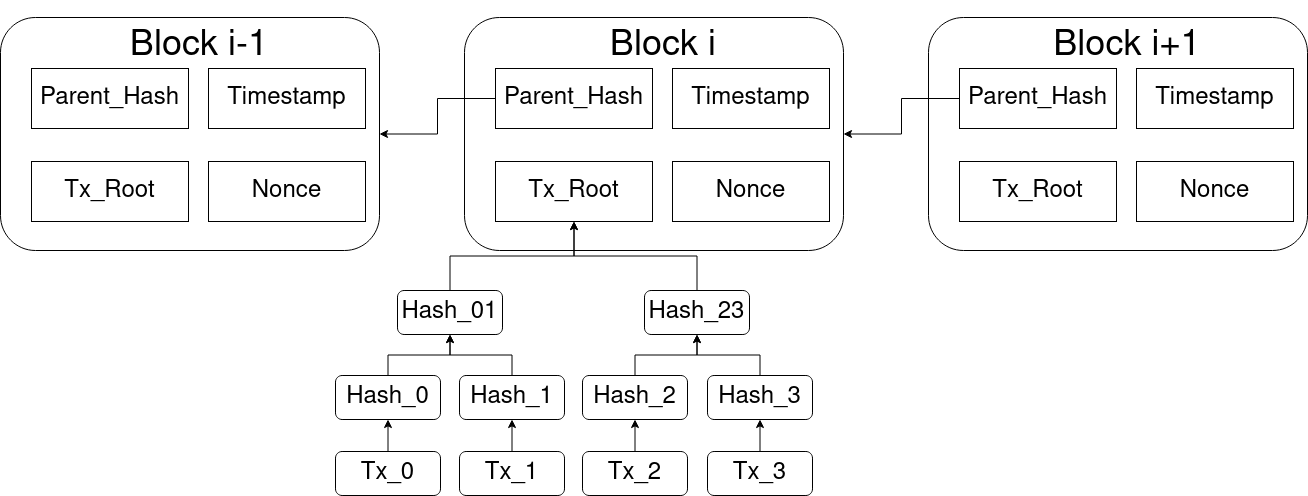
\includegraphics[width=1\columnwidth,keepaspectratio]{figures/blockchain.png}
	\caption{Bitcoin's blockchain data structure.}
	\label{fig:blockchain}
\end{figure}

For the rest of this thesis, we will use the following notation:
\begin{itemize}
    \item $\block$ denotes a block;
    \item $\chain$ denotes a chain of blocks;
    \item $\chain || \block$ denotes the concatenation of a chain and a block;
    \item $\head(\chain)$ denotes the last block of a chain $\chain$, \ie the
        block farthest from genesis \st $\head(\chain || \block) = \block$;
    \item ($\prec$) denotes the prefix operation between two chains; so, if
        $\chain' \prec \chain$, then there exists a chain of blocks $\block_0
        || \dots || \block_j$ such that $\chain = \chain' || \block_0 || \dots
        || \block_j$;
    \item ($\backslash$) denotes the difference of two chains, \eg if $\chain =
        \chain' || \chain''$ then $\chain'' = \chain \backslash \chain'$;
    \item $\chain^{\lceil k}$ denotes the chain obtained by removing the last
        $k$ blocks of chain $\chain$, \ie $\chain \backslash \chain^{\lceil
        k} = \chain'$ where $|\chain'| = k$;
    \item $|\chain|$ denotes the length of chain $\chain$ in blocks;
    \item $\chain[k]$ denotes either the $k$-th block or the $k$-th transaction
        in $\chain$ (depending on the context).
\end{itemize}

Bitcoin Backbone~\cite{EC:GarKiaLeo15,C:GarKiaLeo17} and
subsequently~\cite{EPRINT:KiaPan15} distilled the properties that a secure
blockchain protocol must satisfy (Definition~\ref{def:blockchain-extended}).
Based on these properties and Definition~\ref{def:secure-ledger},
Definition~\ref{def:blockchain} describes the combined, high-level properties
of \emph{persistence} and \emph{liveness} for blockchain-based distributed
ledgers.

\begin{definition}\label{def:blockchain-extended}
    Assume $\totalParties$ parties, each party $\party_i$ locally holding a chain
    $\chain_i = [\tx_{i, 0}, \dots, \tx_{i, j}]$. A secure blockchain protocol
    must satisfy the following properties:
    \begin{itemize}
        \item \emph{Common Prefix}: For parameters $\persistenceParam, \round_0
            \in \mbb{N}$, the chains $\chain_1, \chain_2$ held locally by the
            honest, but not necessarily distinct, parties $\party_1, \party_2$
            at rounds $\round_0 < \round_1 \leq \round_2$ respectively,
            satisfy: $\chain_1^{\lceil \persistenceParam} \prec \chain_2$.
        \item \emph{Chain Quality}: For parameters $l, \mu \in \mbb{N}$, any
            consecutive sequence of $l$ blocks, in a chain held locally by any
            honest party at any point in time, comprises of at least $\mu$
            blocks created by an honest party.
        \item \emph{Chain Growth}: For parameters $s, t \in \mbb{N}$, if at
            round $\round$ an honest party $\party_i$'s chain is
            $\chain_{i, \round}$, then, at round $\round + s$, the chain
            $\chain_{i, \round + s}$ locally held by $\party_i$ satisfies
            $|\chain_{i, \round + s}| \geq \chain_{i, \round} + t$.
    \end{itemize}
\end{definition}

\begin{definition}\label{def:blockchain}
    Assume $\totalParties$ parties, each party $\party_i$ locally holding a chain
    $\chain_i = [\tx_{i, 0}, \dots, \tx_{i, j}]$.

    We call a transaction $\tx$ \emph{stable} if, assuming that for some honest
    party $\party_i$ and some $k \in \mbb{N}$ it holds $\chain_i[k] = \tx$,
    then for every honest party $\party_l$ it holds $\chain_l[k] = \tx$.

    A blockchain-based distributed ledger protocol is secure, with parameters
    $\persistenceParam, \livenessParam$, if it satisfies the following properties:
    \begin{itemize}
        \item \emph{Persistence}:
            For each party $\party_i$, a transaction which is part of a block
            in a prefix chain $\chain_i' \prec \chain$, such that $|\chain_i| -
            |\chain_i'| \geq \persistenceParam$, is stable.
        \item \emph{Liveness}:
            A transaction which is provided as input to an honest party at
            round $\round$ has become stable by round $\round + \livenessParam$.
    \end{itemize}
\end{definition}

The major innovation of Bitcoin~\cite{nakamoto2008bitcoin} was to use a
blockchain to implement a secure distributed ledger under open and dynamic
participation~\cite{EC:GarKiaLeo15,C:GarKiaLeo17,EC:PasSeeShe17}. Up to that
point, distributed ledger
protocols assumed a known number of participating parties; instead, Bitcoin
allows parties to join or leave the protocol as needed. However, in such
open-participation setting, Bitcoin faced two questions: i) how to identify the
party responsible for producing a new block at any stage of the protocol; ii)
how to prevent sybil attacks~\cite{douceur2002sybil}. Briefly, in a sybil
attack an adversary creates a large number of pseudonymous identities to gain
disproportionate power in a system and subvert its security. Bitcoin answered
both these questions with its Proof-of-Work, with other blockchain protocols
following suit with alternatives like Proof-of-Stake.

\paragraph{Proof-of-Work (PoW)}
The core idea behind PoW~\cite{C:DwoNao92} is performing some amount of
computations and then, in order to participate in a protocol, publish a proof
of this ``work'' performed by the hardware. In cryptocurrencies like Bitcoin,
the PoW work is called ``mining''. The mining hardware is provided with two
constants, $\msf{previd}$ and $\msf{data}$, \ie the id of the tip of the
adopted blockchain and the data which need to be appended to it. The mining
device then brute-force searches for some string $\msf{nonce}$, such that
$\hash(\msf{previd} || \msf{data} || \msf{nonce}) \leq T$ for some hash
function $\hash$ defined by the system. $T$ is a --- relatively --- small
number, called the \emph{difficulty target}, which is adjusted to ensure a
stable block production rate, although typically remains constant for periods
of consecutive blocks called epochs. For example, in Bitcoin, epochs are $2016$
blocks long~\cite{SP:BMCNKF15}, while each new block is produced approximately
every $10$ minutes. Because the search for solutions is exhaustive, the
expected number of solutions found by a given miner is proportional to the
number of evaluations of the hash function $\hash$ they can obtain in a given
time frame.

\paragraph{Proof-of-Stake (PoS)}
PoW's deficiencies, particularly its egregious environmental cost, have driven research towards alternative designs,
most prominently Proof-of-Stake (PoS).  In PoS, a minter is selected in
proportion to the stake they hold, which is to say proportionally to the amount
of assets they own.  These assets are managed by the distributed ledger and
serve as both the system's internal currency and consensus participation
tokens.  There exist a number of flavors of this process. In one case, \eg
Ouroboros~\cite{C:KRDO17}, all coins automatically participate in the leader
election process. In a second flavour, the stake has to opt-in to participate
in the election by a special process, such as purchasing a ticket or becoming a
delegate of the stake of other users; this is the case for cryptocurrencies
like Decred~\cite{decred} and EOS~\cite{eosWhitepaper}. PoS systems are almost
energy-free, but often rely on complex cryptographic primitives, \eg secure
Multiparty Computation~\cite{C:KRDO17}, Byzantine
Agreement~\cite{FC:DaiPasShi19,DBLP:conf/sosp/GiladHMVZ17,USENIX:KJGKGF16}, or
Verifiable Random Functions (VRFs)~\cite{EC:DGKR18,DBLP:conf/sosp/GiladHMVZ17}.

Starting with Bitcoin, blockchain-based distributed ledgers are typically used
for financial applications. The ledger acts as a database which records the
ownership of digital assets at any point and the transactions, \ie transfers of
asset ownership, that are performed between users. Each user interacts with the
assets recorded on the ledger via \emph{addresses}.

An address $\addr$ is a string chosen from the set $\addresset \subseteq \{0,
1\}^\addrlen$, where $\addrlen$ is the --- protocol-specific --- address length
parameter. At any point in time, the ledger records the assets that each
address owns. A user controls a single \emph{account}, which may in turn
control multiple addresses; therefore, a user participates in the ledger, via
the account's addresses, in a pseudonymous manner.\footnote{The
literature has also seen a number of fully anonymous blockchain
protocols~\cite{SP:BCGGMT14,SP:MGGR13,EC:CGLMMM17,SP:KKKZ19}, but these are outside
the scope of this thesis.} Intuitively, an address is akin to an IBAN, in
traditional bank accounts. Typically, each address is associated with a payment
key pair $\keypair$, where $\pubkey$ is the public and $\privkey$ the private
key. As explored in Chapter~\ref{chap:delegation}, an address may be associated
with additional data, such as a staking key or metadata. Additionally, in
contract systems like Ethereum, a smart contract may not be associated with a
key pair, but rather only with a piece of software. However, in all cases,
addresses that are maintained by users of the system are associated with at
least one key pair, which is used for receiving and issuing payments.

To transfer assets between addresses, a user creates a transaction $\tx$. In
the simplest case, a transaction comprises of the following objects:
\begin{inparaenum}[i)]
    \item $\addr_s$: the address of the sender, \ie the current owner of the
        assets;
    \item $\addr_r$: the address of the receiver of the assets;
    \item $\asset$: the amount or set of assets which are transferred.
\end{inparaenum}
Typically, the transaction is also signed by the private key associated with
$\addr_s$, such that the sender can prove ownership of the assets. Optionally,
the transaction may also contain additional information, such as a number of
fees, a change address (\ie to receive surplus assets), or metadata (as
explored in Chapters~\ref{chap:hardware-wallets} and~\ref{chap:delegation}).
$\asset$ may be a simple number, if the exchanged assets are fungible, or a set
of individual asset identifiers, in the case of non-fungible assets.

\paragraph{Asset Fungibility}
An asset is fungible if each unit is indistinguishable from the others; in
contrast, each unit of a non-fungible asset is identified by a unique
identifier, which can be used to track it and trace its history. For example,
the US Dollar (USD) is a fungible asset, as citizens transact in amounts of USD
and each single unit of USD is indistinguishable. However, USD bills or
banknotes are non-fungible, since each bill is identified by a unique serial
number, which is often used to track forged or stolen assets. In our work, a
non-fungible asset is identified by a natural number $\asset$, while for
fungible assets we consider only amounts denoted by $\assetset$.

\section{Literature Overview}\label{sec:related}

We now overview notable works that pertain to the entire scope of the thesis.
Following, each individual chapter focuses on the body of literature related to
its specific research questions.

\subsection{Bitcoin Formal Models}
The importance of formal methods for analyzing Bitcoin is well understood, with
existing literature showcasing different approaches. Garay
\etal~\cite{EC:GarKiaLeo15,C:GarKiaLeo17}, after extracting and analyzing the
core Bitcoin blockchain protocol, presented a formal abstraction to prove that
Bitcoin satisfies a set of security and quality properties. Pass
\etal~\cite{EC:PasSeeShe17} analyzed the consistency and liveness properties of
the consensus protocol in an asynchronous setting, proving Bitcoin secure
assuming an upper bound on the network delay. Badertscher \etal~\cite{C:BMTZ17}
suggested a Universally Composable treatment of the Bitcoin ledger, defining
Bitcoin's goals and proving that their model is securely realized in the UC
framework. Transactions, being a core part of Bitcoin, have also attracted
attention; notably, Atzei \etal~\cite{FC:ABLZ18} proposed a formal model of
Bitcoin transactions, to prove security \eg against double-spending attacks.

\subsection{Proof-of-Stake Protocols}
The cryptographic literature has seen a number of PoS protocols in the past
years. A family of such protocols, which was initiated with
Ouroboros~\cite{C:KRDO17} and continued with Ouroboros Praos~\cite{EC:DGKR18},
Ouroboros Genesis~\cite{CCS:BGKRZ18}, and Ouroboros
Crypsinous~\cite{SP:KKKZ19}, provides a wide range of threat model
considerations, relevant to PoS systems, and offers eventual guarantees of
liveness and persistence, similar to Bitcoin.
Algorand~\cite{EPRINT:CGMV18,EPRINT:GHMVZ17} is a protocol which employs
Byzantine Agreement to achieve the necessary properties of a PoS setting, as
well as transaction finality in (expected) constant time. Snow
White~\cite{FC:DaiPasShi19,AC:PasShi17} similarly uses the notion of
``robustly reconfigurable consensus'', which is specially designed to cope with
the lack of participation of users in the consensus protocol.

Real-world PoS implementations often opt for stake representation and
delegation, similar to our work in Chapter~\ref{chap:delegation}.  Systems like
Cardano~\cite{cardano}, EOS~\cite{eosWhitepaper}, and (to
some extent) Tezos~\cite{goodman2014tezos}, employ different consensus
protocols, but all enforce that a (relatively small) subset of representatives
is elected to participate.  Decred~\cite{decred} takes a somewhat different
approach, where stakeholders buy a ticket for participation, akin to PoS with
optional participation. However, these systems typically assume single parties
that act as delegates, either individually or as pool operators, a restriction
that Chapter~\ref{chap:collective-pools} directly aims at relaxing.

\subsection{Blockchain Incentives}
The seminal work of Selfish
Mining~\cite{FC:EyaSir14,FC:SapSomZoh16,kiayias2016blockchain} showed that
honest behavior is not incentive-compatible. However, alternative reward
sharing mechanisms in the PoS setting may make it feasible to perform better in
terms of incentive compatibility. For instance, Ouroboros~\cite{C:KRDO17} can
be designed from the ground up to be a Nash equilibrium under certain plausible
conditions. The question of how to incentivize parties in PoS systems to form a
desired number of stake pools was further studied
in~\cite{DBLP:conf/eurosp/BrunjesKKS20}. The problem that these works study,
and which we also explore in Chapter~\ref{chap:compliance}, is designing the
incentives of blockchain systems from the designer's point of view, so that
participants do not deviate from the prescribed protocol. One related question
is how fair the protocol is to participants themselves, particularly to honest
participants. The Bitcoin Backbone and Selfish Mining works include attacks in
which an adversary can strategically the ledger's performance, causing the
number of blocks and, in turn, the respective rewards, to be disproportionate
to their contributed computational power, thereby harming fairness towards
honest participants. In the PoW setting, Fruitchains~\cite{PODC:PasShi17}
proposes a protocol which solves this problem via the notion of ``fair''
rewards, \ie rewards in exact proportion to the computational power of each
party.


\chapter{
    Formalization of Hardware Wallets
}\label{chap:hardware-wallets}

Bitcoin, being the most successful cryptocurrency, has been repeatedly attacked
with many users losing their funds.  As wallets are the only way for a user to
access their funds, they are repeatedly targeted for attacks that aim to access
the account's keys or redirect the payments, ranging from clipboard
hijacking~\cite{clipboardHijack} and malware~\cite{NDSS:HDMDGM14} to
implementation bugs, \eg the Parity hack in Ethereum~\cite{alois2017ethereum},
and more specific attacks, \eg brain wallets~\cite{FC:VBCKM16}.  In order to
address such threats, different ways to harden the wallet's security have been
proposed, with the most notable one being the utilization of cryptographic
hardware, \ie \emph{hardware wallets}. These specialized devices currently
dominate the market and, as demand grows, so does the number of commercially
available products. However, they are also arguably the least formally studied
part of cryptocurrency ecosystems, with their specifications and security goals
remaining unclear and understudied.

The module known as a hardware wallet is responsible for the account's key
management and the execution of the required cryptographic operations. The
remaining operations are completed by a dedicated software, either provided
together with the hardware or by a third party, with which the hardware
communicates. However, incorporating expensive hardware as a wallet is bound to
bring some security guarantees. Currently, the security of commercially
available products can only be checked through manual inspection of their
implementation, a process that requires a strong engineering and technical
background, and a significant effort and time commitment. In turn, proprietary
assumptions and lack of a universal threat model frequently lead to
implementations prone to attacks.

Our work aims at bridging the gap between formally modeling and verifying the
wallet's properties and claimed specifications. In this chapter, we devise a
formal model which defines the characteristics, specifications, and security
requirements of hardware wallets. Instead of capturing a hardware wallet as a
single module, we conceptualize it as a system of different modules that
communicate with each other to perform the wallet's operations. This approach
allows us to identify a greater set of potential attacks and the conditions for
them to be successful. To that end, we manually inspect commercial products
and extract their implementations, which we then map to our model. As we show,
hardware wallets are prone to a set of attacks and are secure only under
specific, well-defined assumptions. Therefore, our model can not only prove the
security of existing implementations, but also act as a reference guide for
future implementations.

\paragraph{Related work}
Until now, Bitcoin hardware wallets have only been empirically studied, with
research focusing on the integrity of transactions. Gentilal
\etal~\cite{gentilal2017trustzone} stressed the necessity of separating the
wallet into two environments, the trusted and the non-trusted, and proposed
that a wallet remains secure against attacks by isolating the sensitive
operations in the trusted environment. Similarly, Lim
\etal~\cite{lim2014analysis} and Bamert \etal~\cite{bamert2014bluewallet},
argue that security in Bitcoin wallets equals with tamper-resistance and
propose the use of cryptographic hardware. Hardware wallets have not yet been
extensively studied, since no formal attempt to specify the functionalities and
the security properties of such wallets exists so far. As of September 2018,
research  has only focused on attacking commercially available implementations.
Gkaniatsou \etal~\cite{ISC:GkaAraKia17} showed that the low-level communication
between the hardware and its client is vulnerable to attacks which escalate to
the account management.  Their research concluded to a set of attacks on the
Ledger wallets, which allowed to take control of the account's funds.  Hardware
wallets have also been studied against physical attacks.
Volotikin~\cite{volotikin2018bh} showed that specific parts of the Ledger's
flash memory are accessible, exposing the private keys used for the second
factor verification mechanism.  Datko \etal presented fault injection, timing
and power analysis attacks on KeepKey~\cite{keepkey} and Trezor~\cite{trezor},
which allowed them to extract the private key.

\paragraph{Contributions}
This chapter provides a holistic formal treatment of hardware wallets,
identifying their core specifications and security properties.  The proposed
model allows to reason about the offered security of existing wallets and acts
as the foundation for designing and implementing new ones. In particular, this
chapter:
\begin{inparaenum}[i)]
 \item defines the properties and requirements of hardware wallets;
 \item provides a formal model and security guarantees of such wallets;
 \item evaluates the security of commercial products under a formal model.
\end{inparaenum}

In more detail, we identify the properties and security parameters of a Bitcoin
hardware wallet and formally define them in the Universal Composition (UC)
Framework. We present a modular treatment of a hardware wallet, by realizing
the wallet as a set of protocols.  This approach allows us to capture in detail
the wallet's components and interactions, and the potential threats. We deduce
the wallet's security by proving that it is secure under common cryptographic
assumptions, provided that there is no deviation in the protocol execution.
Finally, we define the attacks that are successful under a protocol deviation,
and analyze the security of commercially available wallets.

\section{Formal Model of Hardware Wallets}\label{sec:hw_example}

Bitcoin relies on the Elliptic Curve Signature Scheme (ECDSA) for signing the
transactions and proving ownership of the assets. A Bitcoin account is defined
by a key pair $\keypair$. The public key $\pubkey$ is hashed to create an
address $\addr$ for receiving assets, while the private key $\privkey$ is used
to sign transactions that spend the assets that $\addr$ received. Unauthorized
access to $\privkey$ can result in a loss of funds, thus raising the issue of
securing the account's private keys. A Bitcoin wallet, which offers access to
the network and management of an account, is either implemented via software,
\ie is hosted online by a third party or run locally, or hardware.

The first threat arises from broken cryptographic primitives. For instance, a
broken hash function may allow an attacker to correlate an address with
multiple keys, whereas a broken signature scheme may enable an attacker to
forge transaction signatures, for addresses which it does not own.
Additionally, protecting against unauthorized access to the wallet's operations
has been shown to be as important as using secure cryptographic
primitives~\cite{SP:BMCNKF15,ISC:GkaAraKia17}. To that end, hardware wallets
offer a tamper-resistant and isolated environment for the cryptographic
primitives.

However, a hardware wallet cannot exist in a standalone setting, but rather
requires a client via which it connects to the network. Thus, if the hardware
is connected to a compromised client, any inputs/outputs of the hardware can
potentially be malicious. For example, consider Bob, whose account is defined
by the key pair $\keypair$, and an adversary $\adversary$, who is able to forge
Bob's signature. In this case any signature $\sig_{\adversary}$ of a message
$m_{\adversary}$ chosen by $\adversary$ can be verified by $\pubkey$; hence the
adversary can spend all assets that Bob has previously received, \ie the assets
sent to the hash of $\pubkey$. Let us now assume that Bob's signature is
unforgeable  but $\adversary$ controls the signing algorithm inputs, such that
for any message $m$ that Bob wishes to sign, $\adversary$ substitutes it with
$m_{\adversary}$. Even though the signature is unforgeable, the adversary can
still spend Bob's assets by tampering with the message.

Our model captures the family of attacks which tamper with the inputs/outputs
of the wallet's operations. Thus, as we show, the security of a Bitcoin
hardware wallet is reduced to the security of the underlying cryptographic
primitives \emph{and} the honesty of the three communicating parties, \ie the
hardware, the client, and the user who operates them.

We note that our model does not capture attacks on the network level. In
particular, we assume synchronous communication channels between the
participants of the hardware wallet system, \ie the user, client, and hardware;
this is a natural assumption in this setting, as we expect a direct connection
both between the client and the hardware (\eg via USB) and with the user (via
I/O devices). However, we also assume that, once a transaction is signed and
transmitted by the client, it is published on the ledger within a short time
span. Therefore, our model does not capture possible liveness violations, \eg
delays due to congestion, but rather abstracts the ledger as an ideal module
that satisfies the necessary properties. Nonetheless, a hardware wallet model
that connects to a possibly temporarily insecure ledger would be a useful
enhancement.

\paragraph{The Hardware Wallet Setting}
Software, not being tamper-resistant, cannot guarantee a secure environment for
the wallet's operations. Instead, hardware wallets offer such an environment by
separating the wallet's cryptographic primitives from the other operations, \eg
connection to the Bitcoin network. These devices do not offer network
connectivity; instead they operate in an offline mode. Due to their limited
memory capabilities and the absence of network access, they cannot keep track
of the account's activities, \eg past transactions. Thus, they connect to a
dedicated software, \emph{the client}, which records the account's actions and
provides a usable interface to the user. Hardware wallets operate under the
assumption of a malicious host and provide a trusted path with the user.
Specifically, the hardware displays transaction-related data, which the user
compares to the data presented by the (potentially compromised) client. As
such, the user becomes part of the system and is responsible for identifying
malicious actions by the client.

The wallet operations are initiated by the user, they are executed by the
client, the hardware, or both, and are as follows:
\begin{itemize}
    \item \emph{Setup}: the hardware generates a master key pair
        $\masterkeypair$ and returns the private key $\masterprivkey$, \ie the
        wallet's \emph{seed}, to the user; currently all wallets are
        Hierarchical Deterministic~\cite{CCS:DasFauLos19}, mostly based on the
        BIP32 standard~\cite{bip32}.
    \item  \emph{Session Initialization}: the hardware connects to the client
        and sends to it the master public key $\masterpubkey$;
    \item \emph{Generate Address}: both the client and the hardware generate a
        new address and return it to the user. The hardware derives a key
        pair $(\privkey_i, \pubkey_i)$ from $\masterkeypair$, generates the
        address $\addr_i$ and returns it to the user. The client may either
        generate $\pubkey_i$ using $\masterpubkey$ or receive $\pubkey_i$ from
        the hardware, then generates and stores the corresponding address, and
        finally returns it to the user.
    \item \emph{Calculate Balance}: given a list of the account's addresses,
        the client iterates over the ledger's transactions, calculates the
        account's available assets and returns this amount to the user.
    \item \emph{Transaction Issuing}: the user provides the payment data to the
        client, \ie the amount and receiver's address, which then forwards them
        to the hardware together with the available inputs, \ie the account's
        addresses and balance, and requests its signature. The hardware checks
        whether the inputs belong to the managed account and generates a
        \emph{change address} upon demand, \ie if the balance is larger than
        the payable amount. Then, it requests the user's approval of the
        payment data; if the user confirms the payment, the hardware signs it
        and returns the signature together with the corresponding public key to
        the client in order to publish it on the network.
\end{itemize}
Figure~\ref{fig:user_wallet} illustrates the issuing of a transaction in the
hardware-enhanced wallet setting.

\begin{figure}
    \begin{center}
        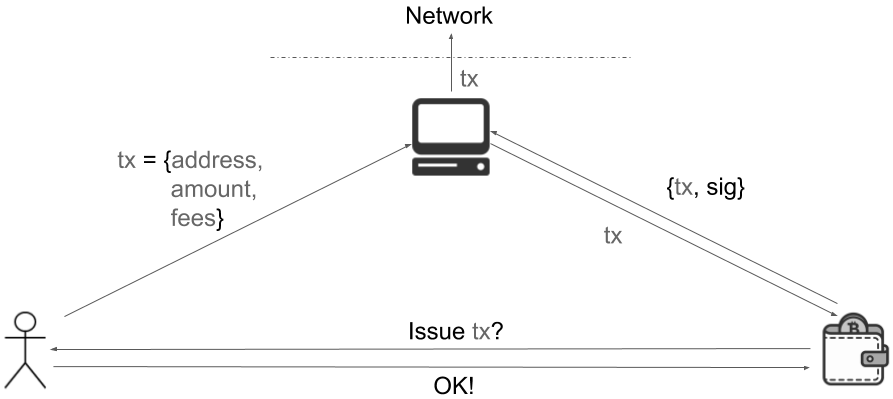
\includegraphics[width=0.75\columnwidth]{figures/hardware-wallets/user_wallet_bw.png}
    \end{center}
    \caption{Transaction issuing in the hardware wallet setting.}
    \label{fig:user_wallet}
\end{figure}

Evidently, a hardware-assisted wallet is not a single module, but rather an
``ecosystem'' of modules that communicate during an operation: the user, the
client, and the hardware. To treat it under the UC framework, we will next
describe an ideal functionality, that defines the wallet's properties, as well
as its real world implementation. In the ideal world, the wallet is a
monolithic component-functionality, responsible for all aforementioned
operations.  In the real world, the wallet emerges through the interaction of
the human operator, the client (\ie a desktop computer, tablet, or smartphone),
and a tamper resistant hardware component. To prove the security of the
real-world protocol, we will compare the two executions (in the real and ideal
settings) and show that they are indistinguishable.

\paragraph{Ideal World}
The wallet functionality, $\Fw$, defines the wallet's operations in the ideal
setting. $\Fw$ interacts with the global Bitcoin ledger functionality $\Gledg$,
as defined in~\cite{C:BMTZ17}, in order to execute operations requiring access
to the decentralized system. $\Gledg$ is the ideal functionality that models
the Bitcoin ledger and allows a wallet to register itself, publish transactions
and retrieve the state of the ledger, \ie all published transactions. $\Fw$
generates a unique address per public key and also incorporates a signature
functionality, $\Fsig$, as defined in~\cite{EPRINT:Canetti03}; for ease of
notation, we show $\Fsig$ as a separate component in the ideal world, although
in fact $\Fw$ simply repeats the steps defined in $\Fsig$. Specifically, the
wallet registers itself with $\Fsig$, which creates fresh keys for the account
upon request, \eg during address generation, and signs messages, \eg
transactions. $\Fsig$ is also accessed by the validation predicate of $\Gledg$,
in order to verify a transaction's signature during the validation stage.

\paragraph{Real World}
The operations defined by $\Fw$ are executed in the real world by a set of
communicating parties: the \emph{hardware}, the \emph{client}, and the
\emph{user}. Thus the protocols of the hardware $\Fhw$, the client $\pclient$,
and the human $\ph$ define the actions of the corresponding parties. The
hardware protocol $\Fhw$, uses a signature scheme $\Sigma \equiv \langle
\algokeygen, \algoverify, \algosign \rangle$, a cryptographic hash function
$\hash$ and a pseudorandom key generation function
$\mathsf{HierarchicalKeyGen}(\masterprivkey, i)$, in order to derive children
keys from the master key. A basic assumption of this setting is that $\pclient$
runs in an untrusted environment, \ie we do not assume the software to be
secure. Thus, in our model, connection to a malicious client is equivalent to
corruption of the client by the adversary. Finally, the user communicates with
the hardware and the client via a secure channel, \ie can interact directly
with the device via buttons and/or a display.

\paragraph{Validation Predicate}\label{sec:validation_predicate}
In both settings, $\Fw$ and the real-world parties have access to a global
Bitcoin ledger functionality $\Gledg$, as defined in~\cite{C:BMTZ17}. $\Gledg$
is parameterized with the validation predicate $\algovalidate$, which
identifies whether a transaction can be added to its buffer, \ie if it is valid
for publishing on the ledger.  The predicate takes as input the candidate
transaction, the buffer, and the current state. The transaction consists of the
signed data $\tx_\sig = (\tx, \pubkey, \sig)$ and ledger parameters, \eg the
transaction id, which is a unique identifier of the transaction, and the
timestamp, \ie the time defined by a global clock. Intuitively, the Bitcoin
state is the blockchain, while the buffer is the mempool, which contains the
transactions that have not yet been included in the blockchain. In our model,
the validation predicate performs the signature verification of a transaction.
This is formalized with a wrapper $\mathsf{ValidateWrapper}$, which wraps all
instantiations of the validation predicate. In the ideal world, the wrapper
accesses the signature functionality $\Fsig$ to verify the transaction's
signature; if the signature is not valid, then it directly outputs $0$,
otherwise it performs all additional checks, such as verifying the consumed
funds and checking the amounts' validity.  The ideal wrapper
$\mathsf{IdealValidateWrapper}$ is described in Algorithm
\ref{alg:validatewrapper}. The real-world wrapper
$\mathsf{RealValidateWrapper}$ uses a signature scheme instead of $\Fsig$ and
behaves similarly to Algorithm \ref{alg:validatewrapper}, \ie it first parses
$\mathsf{BTX}$ and then performs the same branch checks on $\algoverify(\tx,
\pubkey, \sig)$ and returns the proper boolean value.

\begin{algorithm}
    \caption{
        The validation predicate wrapper, parameterized by $\algovalidate$
        and $\Fsig$. The input is a transaction $\mathsf{BTX}$, the buffer
        $\mathsf{buffer}$ and the state $\mathsf{state}$.
    }
    \label{alg:validatewrapper}
    \begin{algorithmic}
        \Function {$\mathsf{IdealValidateWrapper}$}{$\mathsf{BTX, buffer, state}$}
            \State $(\tx, \pubkey, \sig, \msf{txid}, \tau_L, p_i) = \msf{parse}(\mathsf{BTX})$
            \State Send $\msg{Verify}{\tx, \sig, \pubkey}$ to $\Fsig$ and receive $\msg{Verified}{\tx, f}$
            \State \Return $f$
        \EndFunction
    \end{algorithmic}
\end{algorithm}

Finally, Figure~\ref{fig:wallet_worlds} illustrates the ideal and the real
world settings.  In both worlds, the environment $\env$ interacts with the
adversary; Specifically, in the ideal world it interacts with the simulator
$\simulator$ and in the real world with the adversary $\adversary$. In the
ideal world, the wallet consists of the ideal wallet functionality $\Fw$ and
the signature functionality $\Fsig$. In the real world, it consists of the
user, client, and hardware parties, who execute the respective protocols $\ph,
\pclient, \Fhw$.  Communication between the human, client, and hardware is
achieved over a \emph{UC-secure channel protocol}, as presented by
Canetti~\cite{EPRINT:CanKra02a}. Specifically, the adversary is able to observe
the encrypted communication between the honest parties, but can only retrieve
the length of the exchanged messages and not tamper with the plaintext. In
practice, this can be achieved by establishing a secure channel between the
client and the hardware module using standard key exchange techniques, while
the human-hardware channel is assumed to be secure by default. We note that, in
the absence of a secure channel, the adversary may tamper with the
communication, so, in our model, an insecure channel is equivalent to the
client being corrupted.

\begin{figure}
    \begin{center}
        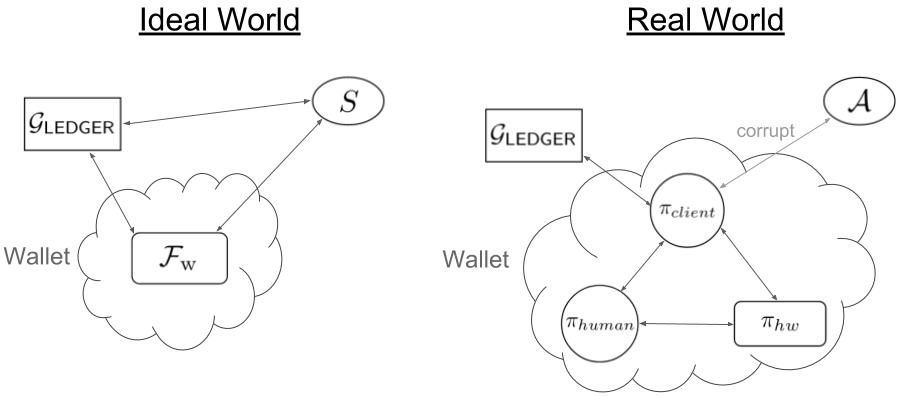
\includegraphics[width=0.80\columnwidth]{figures/hardware-wallets/worlds_bw.png}
    \end{center}
    \caption{A high-level comparison of the ideal and the real worlds.}
    \label{fig:wallet_worlds}
\end{figure}

In the chapter's upcoming sections we use a simplified transaction model, for
ease of notation. Specifically, each transaction defines a single input and
output. We note that adapting it for multiple inputs and outputs, in order to
properly model real-world ledgers, is rather straightforward. The wallet's key
pairs, and consequently its addresses, are generated using the master key pair
$\masterkeypair$, which is randomly selected from the key domain $\keyset$ upon
the wallet's setup. Following, the addresses' keys are derived from a master
key pair as $\privkey_i = \masterprivkey + \hash(i, \masterpubkey)(\bmod$ $n)$
and $\pubkey_i = \masterpubkey + \hash(i, \masterpubkey) \times N$, where $i$
is the index of an address and $n, N$ are public parameters of the Elliptic
Curve. A hardware wallet transaction is a tuple $\tx = (\addr_\msf{s},
\addr_\msf{r}, \asset_\msf{pay}, \addr_\msf{c},
\asset_\msf{change})$. Specifically, $\addr_\msf{s}$ denotes the sender's
address, $\addr_\msf{r}$ the receiver's address, and $\addr_\msf{c}$ the
change address. Additionally, $\asset_\msf{pay}$, $\asset_\msf{change}$
$\asset_\msf{fee}$ are the payment, change and fee funds respectively;
notably, $\asset_\msf{change}$ equals to the account's balance minus the
payment and the fee amounts, \ie $\asset_\msf{change} =
\textrm{balanceOf}(\addr_\msf{s}) - \asset_\msf{pay} -
\asset_\msf{fee}$. A signed transaction is the tuple $(\tx, \pubkey, \sig)$,
where $\sig$ is the signature of $\tx$ under the public key $\pubkey$.  The
parties that execute an operation are the user $\user$, \ie the owner of the
wallet, the client $\client$, \ie the device to which the hardware connects,
and the hardware $\hardware$. Each message is associated with a session id
$\sid' = \user\client\hardware$, which defines the parties with which it is
related.

\section{The Ideal Functionality}\label{sec:fwallet}

$\Fw$ (Figures~\ref{fig:FWallet-1} and~\ref{fig:FWallet-2}) incorporates
$\Fsig$ and runs in the $\Gledg$-setting, interacting with the adversary
$\adversary$, a set of parties $\partyset$, and the environment $\env$. It
keeps the following, initially empty, items:
\begin{inparaenum}[i)]
    \item $A_{[]}$: a list of lists, each containing addresses and their corresponding public keys, $(\addr, \pubkey)$;
    \item $B_{[]}$: a list of lists, each containing addresses and their corresponding balance, $(\addr, \asset)$;
    \item $K_{[]}$: a list of master keys $\masterkeypair$.
\end{inparaenum}
$\Fw$ realizes the following operations, with all messages containing a session
id of the form $\sid = (\partyset, \sid')$:
\begin{itemize}
    \item \emph{Wallet setup}: Upon a setup request, it initializes the list
        of addresses, generates the account's master key, registers to
        $\Gledg$, and returns the master private key to the user.
    \item \emph{Client Corruption}: When $\adversary$ corrupts a client
        $\client$, $\Fw$ leaks the public keys and addresses to which $\client$
        has access.
    \item \emph{Client session initialization}: To start a new session, $\Fw$
        computes and sends to $\client$, defined in $\sid'$, an assigned pass
        phrase; in the real world, the pass phrase acts as the authentication
        mechanism between the parties.
     \item \emph{Address generation}: $\Fw$ requests a new public key from
         $\Fsig$ and picks at random an address, with which to associate the
         key; it then stores the new address in the corresponding list and
         returns it to $\env$. If the client is corrupted, the functionality
         leaks the address and public key to $\adversary$.
    \item \emph{Balance calculation}: If $\client$ is honest, it queries the
        ledger to retrieve the blockchain; if the connected client is
        corrupted, it requests a chain from $\adversary$. Then, it calculates
        the wallet's available assets, based on the provided chain, and returns
        it to $\env$.
    \item \emph{Transaction issuing}: Upon receiving a transaction request, if
        $\client$ is corrupted, $\Fw$ leaks the transaction information to the
        adversary, which responds with a new transaction object. If $\user$ is
        also corrupted, $\Fw$ discards the original request and keeps the
        adversarial transaction, otherwise it ignores the adversary's response.
        Finally, $\Fw$ requests a signature from $\Fsig$ for the accepted
        transaction, which it then sends to $\Gledg$.
\end{itemize}

\myhalfbox{Functionality $\Fw$}{white!40}{white!10}{
    \noindent\emph{Setup:}
        Upon receiving $\msg{Setup}{}$ from some party $\user \in \partyset$,
        forward it to $\adversary$. Then add the empty list $A_{\user}$ to
        $A_{[]}$, register with $\Gledg$, pick the master key pair
        $(\masterprivkey_{\user}, \masterpubkey_{\user}) \xleftarrow{\$}
        \keyset$ and add it to $K_{[]}$ and return $\msg{SetupOK}{}$ to
        $\user$.

    \noindent\emph{Client Corruption:}
        When $\adversary$ corrupts $\client$, send to $\adversary$
        $\msg{AddressList}{A_{\user}}$ and
        $\msg{MasterPubKey}{\masterpubkey_{\user}}$, for every $\user$ such
        that a \emph{Setup} session with $\client$ has been completed.

    \noindent\emph{Initialize Client Session:}
        Upon receiving $\msg{InitSession}{}$ from $\user$, pick $\clId
        \xleftarrow{\$} \{0, 1\}^\secparam$ and send $\msg{InitSession}{\clId}$
        to $\client$. If $\client$ is corrupted, send
        $\msg{InitSession}{\clId}$ to $\adversary$ and wait for a response
        $\msg{InitSessionOK}{\clId}$. Finally, send $\msg{Session}{\clId}$ to
        $\user$.

    \noindent\emph{Generate Address:}
        Upon receiving $\msg{GenAddr}{}$ from $\user$, send $\msg{KeyGen}{}$ to
        $\Fsig$ and wait for a response $\msg{Verification Key}{\pubkey}$.
        Then pick $\addr \xleftarrow{\$} \{0, 1\}^\addrlen$ and add $(\addr,
        \pubkey)$ to $A_{\user}$. If $\client$ is corrupted, send
        $\msg{Address}{(\addr, \pubkey)}$ to $\adversary$ and wait for a
        response $\msg{AddressOK}{\addr'}$. If $\user$ is corrupted, set $a =
        \addr'$, else set $a = \addr$; finally, return $\msg{Address}{a}$ to
        $\user$.

    \noindent\emph{Calculate Balance:}
        Upon receiving $\msg{GetBalance}{}$ from $\user$, send $\msg{Read}{}$
        to $\Gledg$ and wait for a response $\msg{Read}{\chain}$. If
        $\client$ is corrupted, send $\msg{Read}{}$ to $\adversary$ and, upon
        receiving the response $\msg{Read}{\chain'}$, set $\chain = \chain'$.
        Then initialize the list $B_{\user} \in B_{[]}$ with $(a, 0)$ for every
        address $(a, \cdot)$ in $A_{\user}$, and $\forall \tx \in \chain$, \ie
        the ordered transactions in the ledger \st $\tx = (\addr_s, \addr_r,
        \asset_\msf{pay}, \addr_c, \asset_\msf{change})$, do:
        \begin{itemize}
            \item If $\exists (\addr_s, \cdot) \in A_{\user}$, update the entry
                $(\addr_s, \asset_\msf{past})$ $\in$ $B_{\user}$ to $(\addr_s,
                0)$;
            \item If $\exists (\addr_r, \cdot) \in A_{\user}$, update the entry
                $(\addr_r, \asset_\msf{past})$ $\in$ $B_{\user}$ to $(\addr_r,
                \asset_\msf{past} + \asset_\msf{pay})$;
            \item If $\exists (\addr_c, \cdot) \in A_{\user}$, update the entry
                $(\addr_c, \asset_\msf{past})$ $\in$ $B_{\user}$ to $(\addr_c,
                \asset_\msf{past} + \asset_\msf{change})$;
        \end{itemize}
        Finally, compute $b = \sum_{(\cdot, \asset) \in B_{\user}} \asset$ and
        send $\msg{Balance}{b}$ to $\user$.
}{\label{fig:FWallet-1} The ideal hardware wallet functionality. (Part 1)}

\myhalfbox{Functionality $\Fw$}{white!40}{white!10}{
    \noindent\emph{Issue Transaction:}
        Upon receiving $\msg{IssueTX}{(\addr_r, \asset_\msf{pay},
        \asset_\msf{fee})}$ from $\user$, if $\client$ is corrupted,
        forward the message to $\adversary$ and wait for a response
        $\msg{IssueTx}{\clId, (\addr_r', \asset_\msf{pay}',
        \asset_\msf{fee}')}$. If $\user$ is corrupted, set
        $(\addr_r, \asset_\msf{pay}, \asset_\msf{fee}) =
        (\addr_r', \asset_\msf{pay}', \asset_\msf{fee}')$. Then,
        find $(\addr_{in}, \asset_{in}) \in B_{\user}: \asset_{in} \geq
        \asset_\msf{pay} + \asset_\msf{fee}$. If such entry exists,
        do the following:
        \begin{inparaenum}[i)]
            \item compute an address $\addr_c$ and its public key $\pubkey_c$,
                as per the \emph{Generate Address} interface;
            \item set $\asset_\msf{change} = \asset_{in} - \asset_\msf{pay} - \asset_\msf{fee}$
                and $\tx = (\addr_{in}, \addr_{out}, \asset_\msf{pay}, \addr_c, \asset_\msf{change})$;
            \item send $\msg{Sign}{\tx}$ to $\Fsig$ and wait for
                $\msg{Signature}{\tx, \sig}$;
            \item find $(\addr_{in}, \pubkey) \in A_{\user}$ and set
                $\tx_{\sig} = (\tx, \pubkey, \sig)$.
        \end{inparaenum}
        Then, if $\client$ is corrupted, send $\msg{Address}{\addr_c,
        \pubkey_c}$ and $\msg{Submit}{\tx_{\sig}}$ to $\adversary$ and wait for
        the response $\msg{SubmitOK}{}$. Finally, send
        $\msg{Submit}{\tx_{\sig}}$ to $\Gledg$.
}{\label{fig:FWallet-2} The ideal hardware wallet functionality. (Part 2)}

\section{The Real-World Hybrid Setting}\label{sec:hybrid-protocol}

The hybrid setting, which realizes the ideal functionality, consists of the
human $\ph$, client $\pclient$, and hardware $\Fhw$ protocols, each defining
the set of operations run by the corresponding parties.

\paragraph{Human Protocol}\label{subsec:human-protocol}
The user $\user$ interacts with $\client$, $\hardware$, and $\env$, and runs
the protocol $\ph$ (Figure~\ref{fig:PHuman}), which defines
the following, initially empty, items:
\begin{inparaenum}[i)]
    \item $T$: a list of transactions $\tx = (\addr_r, \asset_\msf{pay}, \asset_\msf{fee})$;
    \item $S$: a list of client sessions $\sid$.
\end{inparaenum}
Under the model, a session is initialized when $\user$ connects the hardware
module to the client. $\user$ assigns a random pass phrase $\clId$ to each
client, which is chosen upon session initialization. $\user$ keeps track of the
initiated sessions and pending transactions. However, $\user$ does not perform
complex computations, such as verifying a signature, or maintain a large state,
like the entire list of generated addresses. Instead, $\user$ has a memory $T$,
which contains only the pending transactions, and also is capable of performing
simple computations (like addition/subtraction) and equality checks between
strings.

\myhalfbox{Protocol $\ph$}{white!40}{white!10}{
    \noindent\emph{Setup:}
        Upon receiving $\msg{Setup}{}$ from $\env$, forward it to $\hardware$,
        and initialize $T$ to empty. Then, upon receiving $\msg{SetupOK}{}$ from
        $\hardware$, forward it to $\env$.

    \noindent\emph{Initialize Client Session:}
        Upon receiving $\msg{InitSession}{}$ from $\env$, pick $\clId
        \xleftarrow{\$} \{0, 1\}^\secparam$ and send $\msg{InitSession}{\clId}$
        to $\client$. Upon receiving $\msg{InitSession}{\clId'}$ from
        $\hardware$, if $\clId' = \clId$, add $\clId$ to $S$ and send
        $\msg{Session}{\clId'}$ to $\hardware$ and $\env$.

    \noindent\emph{Generate Address:}
        Upon receiving $\msg{GenAddr}{}$ from $\env$, forward it to $\client$
        and wait for two messages, $\msg{Address}{\addr_{client}}$ from
        $\client$ and $\msg{Address}{\addr_{hw}}$ from $\hardware$.  If
        $\addr_{client} = \addr_{hw}$, send $\msg{Address}{\addr_{hw}}$ to
        $\env$.

    \noindent\emph{Calculate Balance:}
        Upon receiving $\msg{GetBalance}{}$ from $\env$, forward it to
        $\client$. Then, upon receiving $\msg{Balance}{b}$ from $\client$,
        forward it to $\env$.

    \noindent\emph{Issue Transaction:}
        Upon receiving $\msg{IssueTX}{\tx}$ from $\env$, such that $\tx =
        (\addr_r, \asset_\msf{pay}, \asset_\msf{fee})$, add $\tx$ to $T$ and forward
        the message to $\client$. Upon receiving $\msg{CheckTx}{\clId, \tx',
        b'}$ from $\hardware$, if $\clId \in S$, $\tx' \in T$ and
        $b' = b - \asset_\msf{pay} - \asset_\msf{fee}$, remove
        $\tx'$ from $T$ and send $\msg{IssueTx}{\clId, \tx}$ to $\hardware$.
}{\label{fig:PHuman} The ``human'' protocol run by $\user$.}

\paragraph{Client Protocol} \label{subsec:client-protocol}
The client $\client$ interacts with $\user$, the hardware wallet $\hardware$,
and the environment $\env$. The protocol $\pclient$ (Figure~\ref{fig:Pclient})
defines the following items:
\begin{inparaenum}[i)]
    \item $\masterpubkey$: the master public key of the wallet;
    \item $i$: the key derivation index;
    \item $\clId$: the pass phrase assigned by $\user$;
    \item $A_{client}$: a list of the account's addresses;
    \item $T_{utxo}$: a list of address balances.
\end{inparaenum}
$\client$ acts a proxy between $\user$ and $\hardware$, providing connectivity
to the ledger and executing blockchain-related operations, such as computing
the account's balance. During the address generation, $\client$ retrieves the
public key from $\hardware$; in practice this is optional, as $\client$ can
generate an address independently, via the derivation process of the
hierarchical deterministic wallets.

\myhalfbox{Protocol $\pclient$}{white!40}{white!10}{
    \noindent\emph{Initialize Client Session:}
        Upon receiving $\msg{InitSession}{p}$ from $\user$, forward it to
        $\hardware$; upon receiving $\msg{MasterPubKey}{k}$ from
        $\hardware$, set $\clId = p$, $\masterpubkey = k$ and $i = 1$.

    \noindent\emph{Generate Address:}
        Upon receiving $\msg{GenAddr}{}$ from $\user$, forward it to
        $\hardware$. Then, upon receiving $\msg{PubKey}{\pubkey_i}$ from
        $\hardware$, compute $\addr_i = \hash(\pubkey_i)$, set $i = i + 1$, and
        add $\addr_i$ to $A_{client}$. Finally, send $\msg{Address}{\addr_i}$
        to $\user$.

    \noindent\emph{Calculate Balance:}
        Upon receiving $\msg{GetBalance}{}$ from $\user$, send $\msg{Read}{}$
        to $\Gledg$. Upon receiving $\msg{Read}{\chain}$ from $\Gledg$,
        set $T_{utxo}$ to the empty list and
        $\forall \tx \in \chain$, \ie the ordered transactions in the
        ledger \st $\tx = (\addr_s, \addr_r, \asset_\msf{pay}, \addr_c,
        \asset_\msf{change})$, do:
        \begin{itemize}
            \item If $\addr_s \in A_{client}$, update the entry
                $(\addr_s, \asset_\msf{past})\in T_{utxo}$ to $(\addr_s, 0)$;
            \item If $\addr_r \in A_{client}$, update
                $(\addr_r, \asset_\msf{past})\in T_{utxo}$ to $(\addr_r,
                \asset_\msf{past} + \asset_\msf{pay})$;
            \item If $\addr_c \in A_{client}$, update
                $(\addr_c, \asset_\msf{past})\in T_{utxo}$ to $(\addr_c,
                \asset_\msf{past} + \asset_\msf{change})$.
        \end{itemize}
        Finally, compute $b = \sum_{(\cdot, \asset) \in T_{utxo}} \asset$ and
        send $\msg{Balance}{b}$ to $\user$.

    \noindent\emph{Issue Transaction:}
        Upon receiving $\msg{IssueTX}{\tx}$ from $\user$, such that $\tx =
        (\addr_r, \asset_\msf{pay}, \asset_\msf{fee})$, send $\msg{SignTx}{\clId, \tx,
        T_{utxo}}$ to $\hardware$. Upon receiving $\msg{ChangeIndex}{idx}$, set
        $i = idx$ and compute and store the change address and its public key,
        as in the \emph{Generate Address} interface. Then, upon receiving
        $\msg{SignTx}{\tx_{\sig}}$ from $\hardware$, send
        $\msg{Submit}{\tx_{\sig}}$ to $\Gledg$.
}{\label{fig:Pclient} The client protocol run by $\client$.}

\paragraph{Hardware Wallet Protocol}\label{subsec:hardware-protocol}
The hardware $\hardware$ interacts with $\client$ and $\user$ and runs the
protocol $\Fhw$ (Figure~\ref{fig:hardware_protocol}), which defines the
following items:
\begin{inparaenum}[i)]
    \item $i$: the key derivation index,
    \item $S$: a list of the active client sessions,
    \item $\masterkeypair$: the master key pair of the wallet, and
    \item $A$: a list that contains tuples like $(i, \addr_i, \privkey_i,
        \pubkey_i)$, where $i$ is a key derivation index and $\addr_i,
        (\privkey_i, \pubkey_i)$ a generated address and its corresponding key.
\end{inparaenum}
$\hardware$ can perform some specific complex computations, such as hashing or
signature issuing, has limited memory, and completely lacks network connectivity.

\myhalfbox{Protocol $\Fhw$}{white!40}{white!10}{
    \noindent\emph{Setup:}
        Upon receiving $\msg{Setup}{}$ from $\user$, initialize $S$ and $A$ to
        empty lists. Then compute $\masterkeypair \leftarrow
        \algokeygen(1^\secparam)$, set $i = 1$, and return
        $\msg{Setup}{\masterprivkey}$ to $\user$.

    \noindent\emph{Initialize Client Session:}
        Upon receiving $\msg{InitSession}{\clId}$ from $\client$, forward it to
        $\user$. Upon receiving $\msg{Session}{\clId'}$ from $\user$, add
        $\clId'$ to $S$ and send $\msg{MasterPubKey}{\masterpubkey}$ to
        $\client$.

    \noindent\emph{Generate Address:}
        Upon receiving $\msg{GenAddr}{}$ from $\client$, compute $(\privkey_i,
        \pubkey_i) = \msf{HierarchicalKeyGen}(\masterprivkey, i)$ and $\addr_i
        = \hash(\pubkey_i)$. Then, store $(i, \addr_i, \privkey_i, \pubkey_i)$
        to $A$, set $i = i + 1$, and return $\msg{Address}{\addr_i}$ to $\user$
        and $\msg{PubKey}{\pubkey_i}$ to $\client$.

    \noindent\emph{Issue Transaction:}
        Upon receiving $\msg{SignTx}{\clId, \tx, T_{utxo}}$ from $\client$,
        where $\tx = (\addr_r, \asset_\msf{pay}, \asset_\msf{fee})$, find an entry
        $(\addr_{in}, \asset_\msf{in}) \in T_{utxo}: \asset_\msf{in} \geq
        \asset_\msf{pay} + \asset_\msf{fee}$. If such entry exists, then:
        \begin{inparaenum}[i)]
            \item find $(\cdot, \addr_{in}, \privkey_{in}, \pubkey_{in}) \in A$;
            \item compute $\asset_\msf{change} = \asset_\msf{in} -
                \asset_\msf{pay} - \asset_\msf{fee}$;
            \item create an address $\addr_c$, as in the \emph{Generate
                Address} interface;
            \item compute $b = \sum_{(\cdot, \asset) \in T_{utxo}} \asset$ and
                set $b' = b - \asset_\msf{pay} - \asset_\msf{fee}$.
        \end{inparaenum}
        Then, send $\msg{ChangeIndex}{i}$ to $\client$ and $\msg{CheckTx}{\clId,
        \tx', \msf{balance}'}$ to $\user$, where $\tx' = (\addr_r,
        \asset_\msf{pay}, \asset_\msf{fee}')$. Upon receiving $\msg{IssueTx}{\clId,
        \tx}$ from $\user$, set $\tx = (\addr_{in}, \addr_r, \asset_\msf{pay},
        \addr_c, \asset_\msf{change})$, compute $\tx_{\sig} = (\tx, \pubkey_{in},
        \algosign(\tx, \privkey_{in}))$ and send $\msg{SignTx}{\tx_{\sig}}$ to $\client$.
}{\label{fig:hardware_protocol} The hardware protocol run by $\hardware$.}

\section{Security Analysis}\label{sec:theorem}

We now assess the security of the proposed model, to prove the security of the
hybrid setting \wrt $\Fw$. Our model, as defined in $\Fw$, incorporates the
following problematic scenarios:
\begin{enumerate}[1)]
    \item \label{item:privacy} \emph{Privacy loss}: when $\adversary$
        corrupts a client, he accesses the account's public keys, addresses, and
        balance;
    \item \label{item:payment} \emph{Payment attack}: during transaction
        issuing, $\adversary$ may tamper with the inputs to alter the payable
        amounts and/or the receiving address; this attack is successful if
        the client is corrupted \emph{and} the user deviates from their expected
        behavior, \ie does not reject the malicious data;
    \item \label{item:genAdd} \emph{Address generation attack}: $\adversary$
        may tamper with address generation on the client's side, providing an
        adversarial address to the user; again, this attack is successful if
        the client is corrupted \emph{and} the user deviates from their expected
        behavior, \ie does not cross-check the addresses provided by the client
        and the hardware;
    \item \label{item:balance} \emph{Chain attack}: $\adversary$ may tamper
        with the balance calculation by providing a malicious chain to the
        wallet; this family of attacks is successful if only the client is
        corrupted, \ie regardless if the user follows the protocol.
\end{enumerate}

Although the first three scenarios have been previously identified by empirical
studies~\cite{receiveAttack,ISC:GkaAraKia17}, the \emph{chain attack} is more
nuanced. Under our model, the client is the only party that connects to the
network. Therefore, a corrupted client can mount an eclipse
attack~\cite{USENIX:HKZG15}, like the chain attack showcased by the following
example.

Let $\chain_\top$ be the honest chain, \ie the longest chain available on the
network. Also, let $\tx$ be a transaction which transfers $\asset_\msf{in}$
funds to an address $\addr$; $\tx$ is published in the $j$-th block $\block_j$
of $\chain_\top$. Let $\chain \prec \chain_\top$ be a prefix of $\chain_\top$,
which does not include $\block_j$. Also assume that $\chain$ includes a number
of transactions, which transfer an aggregate amount $\asset_\msf{past}$ to
$\addr$. When the hardware requests a chain, the adversary $\adversary$
supplies $\chain$ instead of $\chain_\top$. Hence, during balance calculation,
the wallet assumes that $\addr$ owns only $\asset_\msf{past}$ funds, instead of
the correct amount $\asset_\msf{past} + \asset_\msf{in}$. Following, when the
user attempts to spend the assets owned by $\addr$, the wallet does not consume
the latest UTxO (of $\asset_\msf{in}$ assets), as it is not aware of it.  This
may result in various hazards, from displaying a wrong balance to the user to
failing to recover these funds, \eg if the wallet deletes old (\ie consumed)
addresses.

To prove the security of our model, we show that the hybrid setting of
Section~\ref{sec:hybrid-protocol} (denoted by $\phybrid$) securely realizes the
wallet ideal functionality $\Fw$ of Section~\ref{sec:fwallet}. In the ideal
execution, $\Gledg$ uses the wrapper $\msf{IdealValidateWrapper}$ of
Section~\ref{sec:validation_predicate}, whereas in the real world it
utilizes~$\msf{RealValidateWrapper}$. Theorem~\ref{thm:hybridwallet} is
restricted to environments that do not corrupt the hardware party $\hardware$;
in effect, our analysis does not consider attacks mounted by the hardware's
manufacturer or physical attacks.

\begin{theorem}[Hybrid Wallet]\label{thm:hybridwallet}
    Let the hybrid setting $\phybrid$, which is parameterized by a signature
    scheme $\Sigma$ and a hash function $\hash$, and interacts
    with $\Gledg$, parameterized by $\msf{RealValidateWrapper}$. $\phybrid$
    securely realizes the ideal functionality $\Fw$, which interacts with
    $\Gledg$ parameterized by $\msf{IdealValidateWrapper}$, if and only if
    $\Sigma$ is $\eufcma$ and $\hash$ is an instantiation of the random oracle.
\end{theorem}

\begin{proof}
    \emph{The ``if'' part.}
    For this part of the theorem we assume that the environment $\env$ can
    distinguish between the ideal and the real execution with non-negligible
    probability. We then describe a ``generic'' simulator $\simulator$ for each
    adversary $\adversary$, which emulates the interfaces defined by the
    functionality.  $\simulator$ also runs an internal copy of $\adversary$ and forwards
    the outputs of its computations to $\adversary$. We then construct a forger
    $G$ that runs an internal simulation of the environment $\env$. Thus, for
    each property assumption, we show that there exists a ``bad'' event $E$
    such that, as long as $E$ does not occur, the two executions are
    statistically close. However, when $E$ occurs, the environment $\env$
    distinguishes between the executions. At this point, $G$ uses $\env$ and
    outputs the values that break the property under question. Therefore, since,
    by assumption, $E$ occurs with non-negligible probability, we show that $G$
    is also successful with non-negligible probability.

    \emph{The simulator.}
    Let us now construct the generic simulator $\simulator$. For every
    interface defined by the ideal functionality, $\simulator$ completes the
    operations in the manner defined by the protocols in the hybrid setting. It
    internally runs a copy of the adversary $\adversary$ and forwards the
    necessary messages to it as defined in the hybrid setting. So, the view of
    the $\adversary$ when it interacts with $\simulator$ is the same as in the
    case it operates in the real world setting. $\simulator$ performs as
    follows:
    \begin{itemize}
        \item Any inputs received from the environment $\env$, forward them to
            the internal copy of $\adversary$. Moreover, forward any output from
            $\adversary$ to $\env$;
        \item \emph{Party Setup:} For every party $\party$ for which $\Fw$
            sends messages, spawn an internal simulation of $\user$, $\client$,
            and $\hardware$, which also interact with $\adversary$ as needed
            and run the protocols $\ph$, $\pclient$ and $\Fhw$ respectively;
        \item \emph{Party Corruption:} Whenever the adversary $\adversary$
            corrupts a party, $\simulator$ corrupts it in the ideal process and hands to
            $\adversary$ its internal state;
        \item \emph{(Setup, Initialize Session, Generate Address, Issue
            Transaction):} For any message for these interfaces, follow the
            protocols $\ph$, $\pclient$, and $\Fhw$.
     \end{itemize}

     To prove the theorem regarding the properties of the signature
     scheme we follow the reasoning of Canetti~\cite{EPRINT:Canetti03}. We will
     show the proof for the \emph{unforgeability} property of the signature
     scheme, as the proofs for the other properties follow similarly.

     \emph{Unforgeability.}
     Assume that \emph{consistency} and \emph{completeness} hold for
     $\Sigma$ and $\hash$ instantiates the random oracle. In this
     case, the \emph{Setup, Initialize Session} and \emph{Generate Address}
     interfaces are the same in the both settings from $\adversary$'s point of
     view. Since, by assumption, $\env$ distinguishes between the two, this
     occurs during the \emph{Issue Transaction} phase, \ie by observing a
     valid signature of a transaction which has not been issued by the hardware
     wallet.

     We now construct a forger $G$ that runs a simulated copy of $\env$. $G$
     follows the generic simulator as above, except for the transaction issuing
     interface. Upon receiving $\msg{Submit}{\tx_{\sig}}$, where $\tx_\sig =
     (\tx, \pubkey, \sig)$, it checks if $\algoverify(\tx, \pubkey, \sig) =
     \msf{True}$. If so, it accesses the internal state of the hardware
     $\hardware$ and checks whether it has issued $\tx_{\sig}$. If so, then it
     continues the simulation. Else $G$ outputs $\tx_{\sig}$ as a forgery.
     Since, as long as this does not occur, the two executions are
     statistically close and, by assumption, $\env$ is successful with
     non-negligible probability, then the probability that $G$ is also
     successful is non-negligible.

    \emph{The ``only if'' direction.}
    We show that if one property does not hold, the probability that the
    ``bad'' event $E$ (as above) occurs is non-negligible, so that the
    environment $\env$ can distinguish between the real and ideal executions.
    Again we prove the theorem for the \emph{unforgeability} property, as
    the proofs for the other properties of $\Sigma$ are constructed similarly.
    Also, we conclude the proof with the \emph{address randomness} property,
    which accompanies the assumption that $\hash$ instantiates a random oracle.

     \emph{Unforgeability.}
     Assume that \emph{unforgeability} does not hold for $\Sigma$, \ie there
     exists a forger $G$ for $\Sigma$. When $G$ wishes to obtain a signature for
     some message $m$, the environment sends the message $\msg{IssueTx}{m}$ and
     forwards the response to $G$. When $G$ outputs a forgery $\tx_{\sig} = (\tx, \pubkey,
     \sig)$, if $\tx$ has been previously signed, $\env$ halts. Else it sends
     $\tx_{\sig}$ to $\Gledg$ and observes the ledger's updates. In the ideal
     setting, the transaction will be rejected by the validation predicate and
     will never be included in the ledger. However, in the real world, the
     probability that the transaction is accepted and eventually published in
     the ledger is non-negligible, as the forgery output by $G$ is successful
     with non-negligible probability.

     \emph{Address randomness.}
     Assume that all properties for $\Sigma$ hold. Now, the \emph{Setup,
     Initialize Session} and \emph{Issue Transaction} interfaces are similar in
     both settings. So, if the two worlds are distinguishable, then this is due
     to address generation. Specifically, $\env$ should observe addresses which
     are not uniformly distributed over the space of possible addresses. This
     is impossible in the ideal world, by construction. However, if this was
     true for the real world, then $\hash$ would not instantiate the random
     oracle. Therefore, by assumption, it is impossible for $\env$ to distinguish
     between the two worlds.
\end{proof}

Our model, and the accompanying Theorem~\ref{thm:hybridwallet}, can be used to
prove the security of any hardware wallet that realizes the hybrid setting.
Specifically, to evaluate a wallet implementation, we first need to identified
whether it faithfully realizes the three protocols. Under this premise, the
security assumptions of its building components should be evaluated. More
precisely, the signature algorithm that the wallet uses must be $\eufcma$, the
hash function must simulate the random oracle, and the communication channels
between the parties must be secure. Typical examples of such components are the
\emph{ECDSA}~\cite{johnson2001elliptic} signature algorithm and a
\emph{SHA-2}~\cite{penard2008secure} hash function. If these assumptions hold,
then the wallet is secure under our model.

Finally, one core assumption that deems further investigation is the honesty of
the human user of the wallet. In Section~\ref{subsec:human-protocol}, we
presented a well-defined protocol that the user should follow. As shown in
Section~\ref{sec:theorem}, as long as the parties follow the defined protocols
faithfully, and the cryptographic primitives used are strong enough, the
hardware wallet is secure. The integrity of transaction issuing and address
generation is based, however, on the assumption that the user follows $\ph$
correctly.

$\ph$ requires from the user to identify malicious data, by comparing the data
shown by the client with the data shown by the hardware. In practice, the
presented data is long hexadecimals (\ie Bitcoin addresses). However, even
though such comparison is trivial for software, people are prone to errors.
Comparison of long hexadecimal strings has been proved a challenging procedure,
with research~\cite{hsiao2009study,tan2017can,FC:UzuKarAso07} suggesting that
it is unrealistic to expect a perfect comparison of cryptographic hashes, as
humans find this process difficult. In real world scenarios, the user typically
acts hastily, which often causes deviations from the ``honest'' behavior.
Additionally, expecting the user to manually copy a Bitcoin address from the
hardware's screen defeats the usability purposes of the wallets. Thus, it is
highly possible that the user simply copies the address directly from the
client. Hence, such usability difficulties of the compare-and-confirm process
open an attack vector for the payment and address generation attacks.

We model the probability of a user diverging from $\ph$ as a random variable
$\Hprob$.  The distribution of $\Hprob$ may vary, depending both on the
vigilance of the user and usability parameters. For example, a user allowing
all requests to be completed without checks, \eg because the process takes too
long and the data is difficult to read, demonstrates $\Hprob$ close to $1$. A
user who carefully checks the data, \eg because the hardware presents it in
such way that captures the user's attention, demonstrates $\Hprob$ closer to
$0$. Finally, another factor that affects $\Hprob$ is address length; the
longer the address, the more difficult to read and compare.

\section{Product evaluation}\label{sec:evaluation}

The evaluation of commercial hardware wallet products was performed on September 2018.
At that time, the hardware wallets suggested by
\href{https://bitcoin.org/}{bitcoin.org} were Digital Bitbox, KeepKey, Ledger,
and Trezor. The latter $3$ had an embedded screen to present information to the
user, so we focus on them. We manually inspected these wallets, identified
their protocols, and mapped them to our model.

These implementations bare significant similarities to
each other and our model. Although the wallets did have different low-level
implementations, the protocols that they execute are captured by the hybrid
setting of Section~\ref{sec:hybrid-protocol}. This similarity, between our
model and the actual implementations, reaffirmed the correctness of previous
empirical studies, which suggest that the Ledger wallets are prone to the
payment~\cite{ISC:GkaAraKia17} and address generation~\cite{receiveAttack}
attacks. The wallets were subject to these attacks when the client is dishonest
and secure only if the cryptographic primitives are secure \emph{and} the user
does not deviate from the defined protocol, \ie successfully identifies
tampered data. Moreover, the instantiation of our model to the three
implementations suggests that the wallets were prone to chain attacks, as
discussed in Section~\ref{sec:theorem}.

For each implementation we focused on the two core wallet operations:
\emph{address generation} and \emph{transaction issuing}. Since all
implementations were susceptible to chain attacks, we focused on the viability
of payment and address attacks in each case. We showed that Trezor and KeepKey
were secure against payment and address attacks, as long as the user follows
the protocol and verifies the data, whereas Ledger wallets were prone to
address attacks, due to divergence from our model. We expect this type of
evaluation to become an industry standard for hardware wallets, so that vendors
can improve the security and performance of their products by employing formal
verification methods, instead of empirical techniques.

\paragraph{Trezor and KeepKey}
We investigated the implementation of the Trezor Model T and KeepKey hardware
wallets. Both products are implemented similarly, so we focused only on Trezor.
Trezor provides a touch screen for both displaying information and receiving
input from the user. Based on the developer's guide~\cite{trezor-dev}, we next
describe an abstraction of Trezor's behavior under our model.
During address generation, Trezor requires that the user connects the token to
the client and unlocks it, \ie the user \emph{initiates a session} similar to
our model definition. The client then retrieves the address from the hardware
token and displays it to the user. The hardware also displays the address, as
long as the ``Show on Trezor'' option is enabled. If this option is disabled,
then the user cannot verify the client's address and is prone to an address
attack, \ie the client might display a malicious address which the user cannot
cross-check with the hardware wallet. However, the user manual does urge the
user to always check the two addresses~\cite{trezor-user} to avoid such attack
scenarios.
During transaction issuing, the user again connects the device to the client
and unlocks it. Then they initiate a transaction by giving to the client the
recipient's address, and the payment and fee amounts, similarly to our hybrid
model setting. The client initiates the transaction signing process with the
hardware by providing this data, which the token then displays to the user for
verification. After the user has verified the transaction, the hardware
communicates with the client and signs the needed data. Again, given our high
level investigation, this process matches the communication steps that our
model describes.

\paragraph{Ledger}
We investigate the implementation of Ledger Nano S according to the user
manual~\cite{ledger-manual} and our own analysis. Like Trezor, before
performing any operation the user is required to initiate a session by
connecting the hardware to the client and unlocking it. The hardware provides a
small screen for displaying information and a pair of two buttons for receiving
commands from the user.
During address generation, the client displays the newly generated address to
the user. However, there is no option for the hardware wallet to also display
the address,\footnote{Ledger issued a firmware update to address this issue
and allow both the client and the hardware to generate and display the address;
however, the update process is manual and often
neglected by users.} so that the user can cross-check and verify the
two. This is a clear divergence from our model and allows for address attacks,
\eg by a corrupted client that displays a malicious address to the user.
Transaction issuing is also similar to Trezor and captured by our model. The
user inputs the transaction's data to the client, \ie the recipient's address
and the payment and fee amounts. The client forwards this data to the hardware,
which displays it to the user for verification. After receiving the user's
confirmation, the hardware interacts with the client to sign and publish the
transaction on the blockchain.


\chapter{
    Account Management in Proof-of-Stake Ledgers
}\label{chap:delegation}

Blockchain protocols based on the Proof-of-Stake (PoS) paradigm depend --- by
nature --- on the active participation of stakeholders.  Specifically, in PoS,
the set of potentially eligible parties is comprised of ``stakeholders'', \ie
parties who own some amount of the digital assets which are maintained by the
ledger.  Importantly, this set is open, \ie parties can arbitrarily join and
leave, while also remaining pseudonymous.  Therefore, the eligible party,
dubbed the ``minter'', is selected proportionally to its stake, \ie the amount
of assets that it owns; the details of this selection process have resulted in
a number of PoS flavors and protocols.

However, the inherent {\em duality} of PoS digital assets, which can both be
transferred between entities and used in the protocol's execution, diverges
from the Proof-of-Work (PoW) setting and might result in users abstaining from
engaging in the PoS mechanism.  The stakeholders are expected to consistently
follow the protocol's execution, by checking whether they are eligible to
participate, and, in those cases and within a specific time frame, engage in
transaction processing per the PoS protocol's rules~\cite{C:KRDO17,EPRINT:CGMV18,EPRINT:GHMVZ17,vasin2014blackcoin}. This
feature is in sharp contrast with PoW protocols, which offer a natural
decoupling between the consensus layer participants who generate blocks, \ie
the \emph{miners}, and the users of the system who issue transactions.
Naturally, the set of users subsumes the miners, since \eg the miners collect
fees and may also transact using them, and a substantial number of users do not
participate in the consensus protocol.

This dual nature of PoS assets raises two major considerations. First, some
secret, key-related information is frequently used on behalf of an asset, thus
potentially revealing critical information that weakens the asset's security or
increase the attack surface against a user's wallet. For instance, in the UTxO
model (implemented by Bitcoin), the public key which controls the assets is
published only upon spending them; however, PoS systems cannot adapt this model
directly, since the public key is revealed when participating in the protocol,
\ie (typically) before spending the funds. Therefore, using the same key for
all operations both increases the attack surface against it and introduces
quantum attacks, given that most implementations employ non-post-quantum secure
signature schemes.  Second, a computational and availability requirement is
imposed on the stakeholders; therefore, in an environment where the majority of
users are often offline and abstain from the protocol's execution, the security
guarantees of the ledger are weakened.

The above issues are well-known and have already been informally considered by
the blockchain community. For instance, some schemes propose a separation
between a staking and a payment key to address the first
consideration\footnote{One such discussion is available at:
\url{https://www.reddit.com/r/ethereum/comments/6idf2c}}.  The second
consideration, although seemingly unavoidable given the nature of PoS
protocols, can be countermeasured by enabling the delegation of the PoS
protocol participation rights, \ie block generation and transaction validation.
This mechanism would allow users to organize in ``stake pools'', \ie
consortiums managed by a single user, the pool ``leader'', who participates in
the PoS protocol on behalf of all members. Stake pools bring efficiency
advantages, since the set of stake pool leaders is (typically) smaller than the
entire stakeholders' set. Given that some PoS protocols~\cite{C:KRDO17} are
based on multi-party computation, introducing a \emph{committee} of pool
leaders substantially reduces the computational and communication complexity
overhead.

Interestingly, PoS implementations don't typically address these concerns
comprehensively. On the one hand, ``delegated PoS'', \eg in Steem~\cite{steem}
and EOS~\cite{eosWhitepaper}, attempts to address the second consideration by
enabling the voting of delegates. However, both systems use a single key for
payment and voting, thus failing to address the first consideration.  On the
other hand, systems like NEO~\cite{neo-consensus}, as of September 2020, enabled
only $7$ consensus nodes, $5$ of which are controlled by a single entity,
whereas the only way of participating in the consensus mechanism is via central
approval. Finally, Decred~\cite{decred} uses a ticketing system, \ie
stakeholders buy a ticket to participate in the protocol, which is akin to
using a separate key; however, it requires the locking of funds while staking,
\ie it does not allow concurrent payments and staking, a major blow to the
system's usability.

Evidently, even though practical solutions do exist, a comprehensive and formal
treatment of a PoS system's account management is less well-researched. In
fact, due to the very little systematization of the PoS wallets' security and
the lack of concise guidelines, developers often resolve to ad hoc solutions.
Given that PoS systems are increasingly gaining momentum, it is imperative that
this problem receives a thorough and formal treatment. The results of this
chapter fill this gap by acting as a guideline for system architects and
developers, aiming to better wallet implementations in terms of safety, as well
as enable robust designs with improved performance.  A further important
motivation behind our work is the current low level of decentralization in PoS
systems. As illustrated above, some projects are yet to allow stakeholders to
practice staking, opting instead for a closed set of block producing nodes.
Even in cases where stakeholders are arguably in control of their stake, they
may choose their stake representatives from a very narrow set of accounts; for
instance, the EOS block producing nodes are only $21$ at any given time. Our
work aims at alleviating such centralization tendencies by enabling every user
to either participate on their own or assign their stake to any delegate of
their choice.  Consequently, the formalization of the PoS wallet is a stepping
stone for future research, given that the wallet is the gateway through which
users interact with the system, and a core element of the consensus protocol
itself.  As a result, the composable nature of our framework allows future
research to employ it without composability concerns about its underlying
implementation.

\paragraph{Related Work}
Despite the large number of available PoS cryptocurrencies, formal wallet
research has been rather sparse and limited so far. A widely implemented wallet
standard is the HD Wallet Standard BIP32~\cite{bip32}, based on the idea of
deterministic wallets~\cite{detwallet}. Gutoski and Stebila~\cite{FC:GutSte15}
studied security in the presence of partial key leakage, focusing on
BIP32-compliant wallets, whereas Courtois \etal~\cite{EPRINT:CouEmiVal14}
investigated the state of wallets and key management for
Bitcoin~\cite{nakamoto2008bitcoin}. We note that these works focus on PoW-based
systems and thus do not consider issues such as stake delegation and protocol
participation. In the PoS setting, a related work is the Bitshares' delegation
PoS mechanism~\cite{schuh2017bitshares}, which, however, does not provide any
formal model or proof of security. Furthermore, a formal specification of
Cardano's wallet is also available~\cite{cardano-wallet}, although it focuses
on the wallet's implementation, rather than the security properties and
cryptographic model.

\paragraph{Contributions}
This chapter provides a formal framework of account management and stake
pool formation in PoS systems. In more detail, our contributions are as
follows. First, we present the relevant desiderata of a PoS wallet, \ie a set
of requirements general and flexible enough to be compatible with a number of
different types of actors in the system. Based on the desiderata, we provide a
formal treatment of address and asset management in the form of the ideal
functionality $\FuncW$, which epitomizes a PoS wallet's core. Our analysis
follows in the tradition of the UC Framework~\cite{FOCS:Canetti01} and is
inspired by Canetti~\cite{EPRINT:Canetti03}, which allows us to define our
setting in a composable way. While formalizing the addresses and their
attributes, a nuanced and overlooked, but equally important, notion emerges,
namely \emph{address malleability}. This property is also of independent
interest for any setting where an object, such as an identification tag,
depends on multiple attributes, such as keys or metadata.  We describe various
threat models and protection levels, which range from fully malleable schemes
to entirely non-malleable.  Given our theoretical foundations, we next define
the wallet protocol, which securely realizes $\FuncW$ under standard
cryptographic assumptions. The protocol is highly parametric, thus offering
flexibility in the wallet's implementation. Following, we describe an address
construction mechanism, which both ensures a strong level of security and
covers the majority of our desiderata. Finally, we combine the core wallet
funcitonality with a generic PoS ledger to form a complete PoS wallet.
Specifically, we detail how the core wallet can participate in the PoS protocol
and conduct payments, stake pool registration, and stake delegation, and
conclude with proving the security of the stake-pooled variant of any PoS
protocol, as well as describe various modes of operation, which allow for
enhanced privacy and security.

\section{General Desiderata}\label{sec:desiderata-delegation}

Before presenting our framework, we first identify the properties that the
wallet in a PoS setting should offer. This investigation is an important step
in understanding the restrictions in designing such systems, as well as
evaluating the choices that a PoS protocol's designer should make. We organize
the desiderata in three basic categories, based on the related system
component.

\paragraph{Addresses and Attributes}\label{subsec:address-desiderata}
In a PoS system, each account manages a set of addresses. These addresses own a
non-negative amount of cryptocurrency assets and may contain various account
metadata. Any PoS system should offer at minimum two basic operations for each
user's account:
\begin{inparaenum}[i)]
    \item \emph{paying} and
    \item \emph{staking}.
\end{inparaenum}
Addresses, simply put, are strings which have cryptocurrency balances
associated with them. They may also contain metadata, in the form of arbitrary
attributes, which are useful for various system operations. We identify the
following desiderata for addresses in a PoS setting:
\begin{itemize}
    \item \emph{Address Non-malleability}: assuming access to an address and
        the ledger, an adversary should not be able to construct a different
        address that shares \emph{only some} of the address's attributes;
    \item \emph{Address Uniqueness}: any two addresses with different
        attributes should be distinct;
    \item \emph{Short Addresses}: addresses should be relatively short (in
        order to be usable and storage efficient);
    \item \emph{Multiple Types of Addresses}: construction of more than one
        type of addresses should be allowed, with each type supporting a
        different subset of basic operations (\eg to ban some addresses from
        participating in consensus);
    \item \emph{Multiple Device Support}: an account should be able to exist on
        multiple devices that share \emph{no joint internal state};
    \item \emph{Address Recovery}: an account should be able to identify its
        addresses, assuming access to the ledger and the payment keys which it
        controls;
    \item \emph{Privacy and unlinkability:} addresses should be
        indistinguishable from one another and not publicly-linkable to their
        account.
\end{itemize}

\paragraph{Basic Account Operations}
The two basic types of operations, \ie \emph{payment} and \emph{staking}, can
be performed independently by two separate pieces of information, denoted by
$\accPay$ and $\accSta$. The main advantage of this approach is that $\accPay$ is
reserved only for transferring funds, while staking operations require access
only to $\accSta$.  Another desirable result is the ability to recover all
addresses given a master key, \eg as implemented by HD
Wallets~\cite{CCS:DasFauLos19,FC:GutSte15,bip32}; this feature is particularly
important in case the equipment which hosts the wallet is lost. We summarize
the above, with some additions, as follows:
\begin{itemize}
    \item \emph{Account Master Key:} there should exist a ``master'' piece of
        information, \eg a master seed, that can be used to generate all of the
        account's management information, \ie its keys;
    \item \emph{Staking and Payment Separation:} compromising the staking
        operations should not affect the payment operations (and vice-versa);
    \item \emph{Payment Key Information Safety:} apart from a cryptographic
        hash, no other information about the payment key $\accPay$ should be
        public prior to issuing a payment;
    \item \emph{Key Exposure Mitigation:} ownership of the account's assets and
        staking ability should be recoverable, in case the staking information
        $\accSta$ is compromised.
\end{itemize}

\paragraph{Delegation Mechanism and Stake Pools}
Delegation depends on the ability of a user to give the rights over her stake
to another user. This action should be distinguishable from other actions, like
payment, in order to protect the users and facilitate automatic reward schemes.
Therefore, the delegation desiderata are as follows:
\begin{itemize}
    \item \emph{Cost Effectiveness:} stake delegation, re-delegation, or pool
        formation should be cost effective;
    \item \emph{Chain Delegation Restriction:} a limit to the number of
        re-delegations of the same stake unit should be enforceable;
    \item \emph{Delegation Verification:} participants in the system should be
        able to verify the status of active delegations.
\end{itemize}

\section{Address Malleability}\label{subsec:malleability_predicate}

We first introduce the notion of address malleability. We describe the
adversarial threat models that might exploit it, distill the components that
define a malleability attack, and organize this family of attacks based on
threat levels. Next, we formalize malleability via the \emph{malleability
predicate} and present a formal addressing of these attacks. Before proceeding
with the definition though, we first define the objects that underpin our
constructions and explore the malleability of addresses.

An \emph{account} comprises of multiple addresses.  An address is associated
with a number $\addrgenlength$ of \emph{attributes}, each identifying a
property of the address, which are organized as follows:
\begin{inparaenum}[i)]
    \item \emph{public} attributes are part of the address, so they are public
        and available without any interaction with the account's owner;
    \item \emph{semi-public} attributes are not public by default, but become
        public when a transaction is issued, which spends some assets that the
        address owns;
    \item \emph{private} attributes never become public.
\end{inparaenum}
An \emph{attribute list} $l$ is a vector of $\addrgenlength$ attributes. In our
work, the fundamental list of attributes is the \emph{address generation list}
$\addressgenlist$, \ie the list of all attributes used during the generation of
an address $\addr$. In this list, the sub-list of public attributes $d =
(\attribute_1, \ldots, \attribute_{p-1})$ contains the attributes which are
available by every party with access to the address. Of the remaining
attributes, the sub-list $(\attribute_p, \ldots, \attribute_{i-1})$ contains
the semi-public attributes, while $(\attribute_i, \ldots,
\attribute_\addrgenlength)$ contains the private attributes. The parameters $p$
and $i$ depend on the inner workings of the protocol and the address generation
scheme. For example, in Bitcoin, a typical address attribute is the payment key
pair $\paymentkeypair$: $\paymentkeyverify$ is used to verify signatures and is
\emph{semi-public}, its hash is a \emph{public} attribute, whereas
$\paymentkeysign$, which signs transactions, is \emph{private}.

Before exploring address malleability, a brief motivation is necessary. Address
malleability is similar to the preexisting malleability
notions~\cite{dolev2003nonmalleable} and is intrinsically tied to address
generation. Here, we treat it as a novel family of attack vectors due to the
complex structure of PoS addresses. Namely, our framework's addresses encode
information that extend beyond the simple transfer of assets and pertain to
additional functionalities, like staking. Therefore, to ensure the PoS
protocol's security, it is crucial to prevent an adversary $\adversary$ from
constructing addresses on behalf of honest users, or manipulating honestly
generated addresses.

The goal of $\adversary$ is to inflate their stake in the system by exploiting
address malleability. We remind that an address is associated with the payment
information $\accPay$, which is used to issue payments (and practically
controls the assets) and the staking information $\accSta$, which is used to
participate in the PoS consensus protocol. $\adversary$ attempts to forge an
address, for which it controls the staking information $\accSta$ without
controlling the payment information $\accPay$. This results in a stake
``shift'', via which $\adversary$ gains illegitimate control of the staking
rights of assets it does not own.  Importantly, this forgery should take place
in such a way that the address's honest owner does not easily recognize this
stake shift, unless actively looking for it.

Numerous types of adversaries would try to exploit this hazard.  One such type
is a malicious stake pool leader. Such attacker would operate under the ---
natural --- assumption that the reward amount depends on the stake percentage,
the staking rights of which the pool controls. This assumption is amplified
given incentives mechanisms~\cite{DBLP:journals/corr/abs-1807-11218} which
mandate that larger stake pools receive greater rewards. By deploying a
generalized malleability attack, $\adversary$ would artificially increase the
amount of its rewards (Figure~\ref{fig:malleability_attack}). To deploy this
attack, $\adversary$ could intercept honestly-generated addresses, which are
exchanged between users, and replace them with forged addresses which are
created on-the-fly. As long as $\adversary$ remains unnoticed, it may be very
profitable to mount such attack on a broad network level.

\begin{figure}
  \begin{center}
    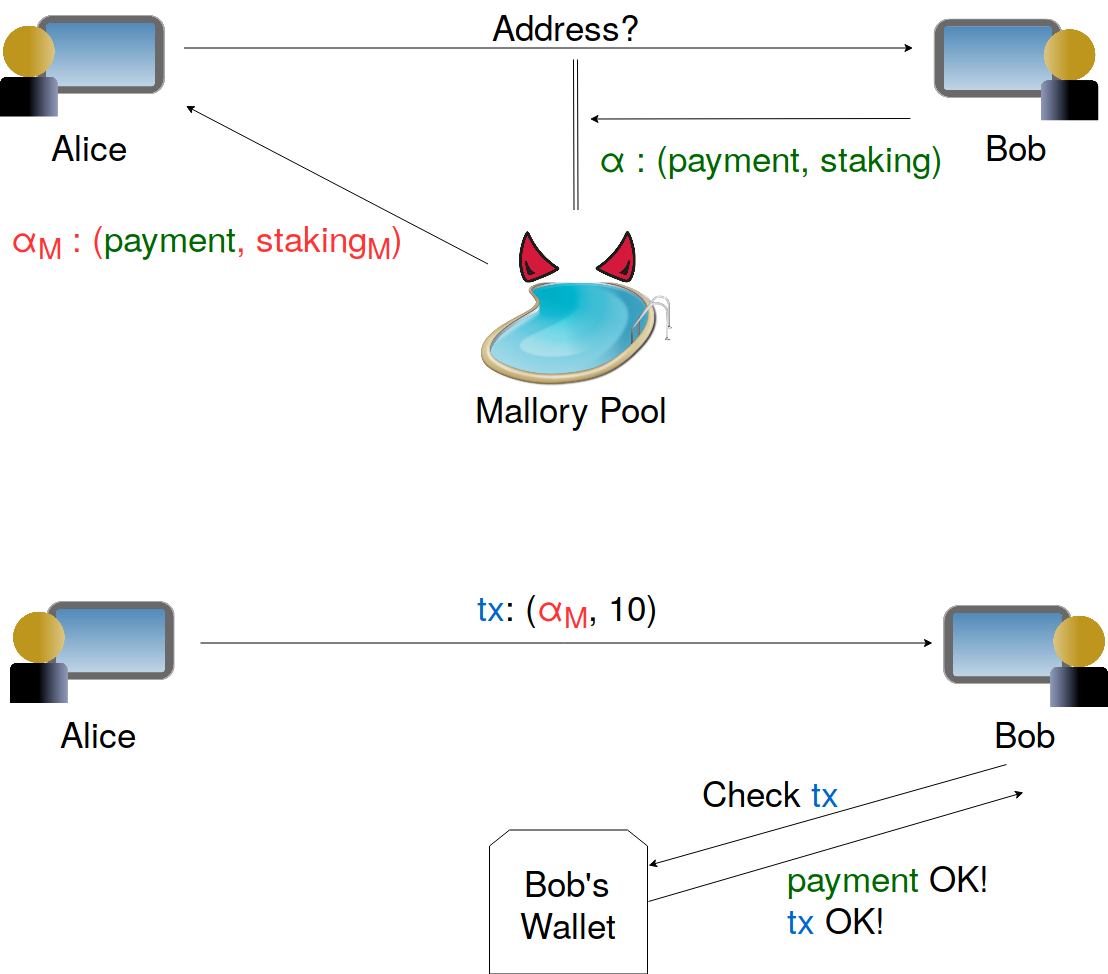
\includegraphics[width=0.6\textwidth]{figures/delegation/malleability_attack.png}
  \end{center}
  \caption{
      An example of a network-level, Man-in-the-Middle malleability attack. A
      malicious pool changes on-the-fly the staking object of one of Bob's
      addresses, such that it points to Mallory's stake pool. If Bob's wallet
      does not identify the attack, Mallory has successfully (but artificially)
      inflated its delegated stake. If the wallet does identify the attack, it
      has to transfer the funds to a correct address and impose extra fees on
      Bob.
    }
  \label{fig:malleability_attack}
\end{figure}

Following we identify multiple types of address malleability attacks. In all
cases, we assume that the adversary does not control the signing payment key
$\paymentkeysign$, as this would trivialize all attacks. An address created by
$\adversary$ without access to its payment key is called \emph{forgery}. A
forgery is successful if funds that are sent to it can be spent and the wallet
accepts the forged address as its own, whereas it fails if funds that are sent
to it can never be spent and are, therefore, ``burnt''.

Our analysis assumes two types of adversaries, depending on the level of
information which they access. First is the \emph{network adversary}, who has
access to the ledger, observes the network, and can intercept addresses
exchanged between parties. Second is the \emph{targeting adversary}, with
access to the same information as the first, but also knows the set of past
transactions issued by the ``victim'', \ie the honest user for which it
attempts to produce a forgery. We stress that the assumptions for the targeting
adversary are much stronger compared to the network adversary.

The malleability levels presented next range from \emph{full malleability}, \ie
when no inherent protection against malleability attacks exists, to \emph{non
malleability}, \ie where an adversary cannot create a successful forgery
without access to the address's private attributes. Defining the intermediate
levels allows us to construct various address schemes, which are suitable for
different needs of real world projects.  For example, a fully malleable address
is typically short and suitable for performance-oriented applications.  In
contrast, a security-oriented project would aim for the higher levels of
malleability protection. The malleability levels are organized around the
following three properties:
\begin{inparaenum}[i)]
    \item the type of adversary, \ie $\adversary$ is at the network level or
        has targeted access to the user's wallet;
    \item self-verification, \ie whether a wallet can recognize a forgery
        for one of its own payment keys;
    \item cross-verification, \ie whether a wallet can identify a forgery
        for an address which it does not own.
\end{inparaenum}
Below we describe the malleability levels and summarize them in
Table~\ref{tab:malleability_levels}:
\begin{itemize}
    \item \emph{Level 1, Full Malleability:} This level enables successful
        forgeries from both network and targeting adversaries. A wallet checks
        only the payment information, so it accepts the forgery without
        recognizing it as such, while also both spending from and sending funds
        to forgeries.
    \item \emph{Level 2, Full Verifiable Malleability:} Again, both types of
        adversaries, \ie network and targeting, can create forgeries. However,
        during recovery, the wallet identifies forgeries and rejects them; we
        note that a ``hacked'' wallet can spend the assets
        owned by such forgery. Also all wallets, including honest ones, may
        send funds to forgeries.
    \item \emph{Level 3, A Posteriori Malleability:} This level prohibits
        network adversaries. Specifically, if such adversary produces a
        forgery, any transaction which spends from the forgery is rejected.
        However, targeting adversaries can create successful forgeries as
        before.
    \item \emph{Level 4, A Posteriori Verifiable Malleability:} This level is
        similar to \emph{Level 3}, with the addition that an honest wallet can
        identify and reject forgeries of its own addresses, as in \emph{Level
        2}.
    \item \emph{Level 5, ``Sink'' Malleability:} Both network and targeting
        adversaries are prohibited. Thus, all forgeries are rejected by the
        wallet and its funds are burnt. Intuitively, considering
        transactions as a graph, where the graph's nodes are the addresses and
        its edges are transactions, forgeries are ``sinks'' which trap all
        funds sent to them. However, a wallet still cannot identify a forgery
        of an address that it does not own.
    \item \emph{Level 6, Non Malleability:} The highest level of
        protection against malleability, where a forgery is rejected by every
        wallet, \ie given only an address anybody can identify whether it is
        honestly-generated or a forgery. Therefore, all transactions that
        interact in any way with a forgery are rejected.
\end{itemize}

\begin{table}[]
\centering \def\arraystretch{1.5}

\begin{center}
  \begin{tabular}{|c|c|c|c|c|}
    \cline{1-5}
          \multicolumn{1}{|c|}{\begin{tabular}[c]{@{}c@{}} Level of \\ Malleability \end{tabular}}
        & \multicolumn{1}{c|}{\begin{tabular}[c]{@{}c@{}} Network \\ protection \end{tabular}}
        & \multicolumn{1}{c|}{\begin{tabular}[c]{@{}c@{}} Targeting \\ protection \end{tabular}}
        & \multicolumn{1}{c|}{\begin{tabular}[c]{@{}c@{}} Self-\\verification \end{tabular}}
        & \multicolumn{1}{c|}{\begin{tabular}[c]{@{}c@{}} Cross-\\verification \end{tabular}} \\
    \hline
       \multicolumn{1}{|l|}{\begin{tabular}[c]{@{}c@{}} 1 - Full \end{tabular}}
     & \multicolumn{1}{c|}{\begin{tabular}[c]{@{}c@{}} \xmark \end{tabular}}
     & \multicolumn{1}{c|}{\begin{tabular}[c]{@{}c@{}} \xmark \end{tabular}}
     & \multicolumn{1}{c|}{\begin{tabular}[c]{@{}c@{}} \xmark \end{tabular}}
     & \multicolumn{1}{c|}{\begin{tabular}[c]{@{}c@{}} \xmark \end{tabular}} \\
    \hline
       \multicolumn{1}{|l|}{\begin{tabular}[c]{@{}c@{}} 2 - Verifiable  \end{tabular}}
     & \multicolumn{1}{c|}{\begin{tabular}[c]{@{}c@{}} \xmark \end{tabular}}
     & \multicolumn{1}{c|}{\begin{tabular}[c]{@{}c@{}} \xmark \end{tabular}}
     & \multicolumn{1}{c|}{\begin{tabular}[c]{@{}c@{}} \cmark \end{tabular}}
     & \multicolumn{1}{c|}{\begin{tabular}[c]{@{}c@{}} \xmark \end{tabular}} \\
    \hline
       \multicolumn{1}{|l|}{\begin{tabular}[c]{@{}c@{}} 3 - A posteriori  \end{tabular}}
     & \multicolumn{1}{c|}{\begin{tabular}[c]{@{}c@{}} \cmark \end{tabular}}
     & \multicolumn{1}{c|}{\begin{tabular}[c]{@{}c@{}} \xmark \end{tabular}}
     & \multicolumn{1}{c|}{\begin{tabular}[c]{@{}c@{}} \xmark \end{tabular}}
     & \multicolumn{1}{c|}{\begin{tabular}[c]{@{}c@{}} \xmark \end{tabular}} \\
    \hline
       \multicolumn{1}{|l|}{\begin{tabular}[c]{@{}c@{}} 4 - A posteriori \\ verifiable  \end{tabular}}
     & \multicolumn{1}{c|}{\begin{tabular}[c]{@{}c@{}} \cmark \end{tabular}}
     & \multicolumn{1}{c|}{\begin{tabular}[c]{@{}c@{}} \xmark \end{tabular}}
     & \multicolumn{1}{c|}{\begin{tabular}[c]{@{}c@{}} \cmark \end{tabular}}
     & \multicolumn{1}{c|}{\begin{tabular}[c]{@{}c@{}} \xmark \end{tabular}} \\
    \hline
       \multicolumn{1}{|l|}{\begin{tabular}[c]{@{}c@{}} 5 - Sink  \end{tabular}}
     & \multicolumn{1}{c|}{\begin{tabular}[c]{@{}c@{}} \cmark \end{tabular}}
     & \multicolumn{1}{c|}{\begin{tabular}[c]{@{}c@{}} \cmark \end{tabular}}
     & \multicolumn{1}{c|}{\begin{tabular}[c]{@{}c@{}} \cmark \end{tabular}}
     & \multicolumn{1}{c|}{\begin{tabular}[c]{@{}c@{}} \xmark \end{tabular}} \\
    \hline
       \multicolumn{1}{|l|}{\begin{tabular}[c]{@{}c@{}} 6 - None  \end{tabular}}
     & \multicolumn{1}{c|}{\begin{tabular}[c]{@{}c@{}} \cmark \end{tabular}}
     & \multicolumn{1}{c|}{\begin{tabular}[c]{@{}c@{}} \cmark \end{tabular}}
     & \multicolumn{1}{c|}{\begin{tabular}[c]{@{}c@{}} \cmark \end{tabular}}
     & \multicolumn{1}{c|}{\begin{tabular}[c]{@{}c@{}} \cmark \end{tabular}} \\
    \hline
  \end{tabular}
\end{center}
\normalsize
\caption{Comparison of the malleability levels.}\label{tab:malleability_levels}
\end{table}

We now formalize address malleability with the predicate $M$. The predicate
returns $1$ or $0$ to denote whether an address is valid or not.  Here, a valid
address is either honestly-generated or a successful forgery, \ie it is an
address that the wallet accepts. The first parameter of the predicate is the
set $L_{\party}$ of all created addresses and their attributes for a party
$\party$; this parameter is necessary, so that the predicate compares the given
address with the honestly generated ones. The second parameter is the auxiliary
information $\msf{aux}_M$, which takes the values $\msf{recover}$ $\msf{issue}$ or
$\msf{verify}$ this information is used to instantiate different modes of the
predicate and allows it to adjust its actions, thus making it more versatile.
The third parameter is the address under question.

\paragraph{Full Malleability}
This predicate does not allow the ideal functionality to perform any
malleability checks when issuing a transaction. During recovery and
verification, it first identifies the list of public attributes $d$, then
outputs $1$ if these attributes have been used in at least one address that the
wallet controls. Intuitively, a forgery can be constructed by using public
attributes from other addresses that the wallet has created. In the real-world,
the wallet accepts an address as long as its payment key is controlled by the
wallet. In a \emph{fully malleable} construction, the predicate is instantiated
with $M_{\mathsf{FM}}$ described in Algorithm \ref{algo:fm_predicate}; the
function $\mathrm{parsePubAttrs}$ denotes the public attribute parsing  of an
address.

\begin{algorithm}
    \caption{The \emph{fully malleable} predicate. The inputs are: i) a list of tuples of previously-generated addresses and their attributes, ii) auxiliary information on the wallet's operation, iii) the address under question.}\label{algo:fm_predicate}
    \begin{algorithmic}
        \Function{$M_{\mathsf{FM}}$}{$L_P, \msf{aux}_M, \addr$}
            \Switch{$\msf{aux}_M$}
                \Case{$\msf{issue}$}
                    \State \Return 1
                \EndCase
                \Case{$\msf{verify}$ OR $\msf{recover}$}
                    \State $d = \textrm{parsePubAttrs}(\addr)$
                    \For {$\attribute \in d$}
                        \If {$\forall \addr' \in L_P, d' = \textrm{parsePubAttrs}(\addr')$: $\attribute \not \in d'$}
                            \State \Return 0 \Comment{$\attribute$ not registered detected}
                        \EndIf
                    \EndFor
                \EndCase
            \EndSwitch
            \State \Return 1
        \EndFunction
    \end{algorithmic}
\end{algorithm}

\paragraph{A Posteriori Malleability}
In an \emph{a posteriori malleable} construction, the predicate first
identifies the list $d$ of public attributes of the address $\addr$.  Then, for
each such attribute $\attribute$, it checks:
\begin{inparaenum}[i)]
    \item if there exists an issued transaction $\tx = (\assetset, \addr_s,
        \addr_r, m)$, such that the public attributes of $\addr_s$ include
        $\attribute$;
    \item if there exists an address that the wallet has created, such that
        $\attribute$ is part of its public attributes.
\end{inparaenum}
If both checks fail the predicate returns $0$, otherwise $1$.  Intuitively,
this construction enables malleability only for addresses whose payment key has
been previously used and for which all public attributes have been used in
other addresses. Therefore, as long as the payment key of the address has not
been used, the scheme provides non-malleability. The \emph{a posteriori
malleable} construction, instantiated with the predicate
$M^{\mathbb{T}}_{\mathsf{PM}}$ which is parameterized by the list of all
transactions $\mathbb{T}$, is described in Algorithm \ref{algo:pm_predicate}.

\begin{algorithm}
    \caption{The \emph{a posteriori} malleability predicate. The inputs are: i) a list of tuples of previously-generated addresses and their attributes, ii) auxiliary information on the wallet's operation, iii) the address under question.}\label{algo:pm_predicate}
    \begin{algorithmic}
        \Function {$M^{\mathbb{T}}_{\mathsf{PM}}$}{$L_P, \msf{aux}_M, \addr$}
            \Switch{$\msf{aux}_M$}
                \Case{$\msf{issue}$}
                    \State \Return 1
                \EndCase
                \Case{$\msf{verify}$ OR $\msf{recover}$}
                    \State $d = \textrm{parsePubAttrs}(\addr)$
                    \For {$\attribute \in d$}
                        \If {$\forall \addr' \in L_P, d' = \textrm{parsePubAttrs}(\addr')$: $\attribute \not \in d'$}
                            \State \Return 0
                        \EndIf
                        \If {$\forall (\assetset, \addr_s, \addr_r, m) \in \mathbb{T}, d_s = \textrm{parsePubAttrs}(\addr_s)$: $\attribute \not \in d_s$}
                            \State \Return 0
                        \EndIf
                    \EndFor
                    \State \Return 1
                \EndCase
            \EndSwitch
        \EndFunction
    \end{algorithmic}
\end{algorithm}

\paragraph{Sink Malleability}
Intuitively, a \emph{sink malleable} address generation algorithm requires that
only the owner of the honest wallet can create addresses for payment keys of
the wallet. This is expressed by differentiating the behavior depending on the
auxiliary information. If $\msf{aux}_M$ pertains to the issuing of transactions, the
predicate returns $1$, \ie accepts all addresses to which the wallet tries to
send funds. For all other cases, it requires that the address is honestly
generated. The sink malleable construction, with the predicate
$M_{\mathsf{SM}}$, is described in Algorithm \ref{algo:sm_predicate}.

\begin{algorithm}
    \caption{The \emph{sink malleable} predicate. The inputs are: i) a list of tuples of previously-generated addresses and their attributes, ii) auxiliary information on the wallet's operation, iii) the address under question.}\label{algo:sm_predicate}
    \begin{algorithmic}
        \Function {$M_{\mathsf{SM}}$}{$L_P, \msf{aux}_M, \addr$}
            \Switch{$\msf{aux}_M$}
                \Case{$\msf{issue}$}
                    \State \Return 1
                \EndCase
                \Case{$\msf{verify}$ OR $\msf{recover}$}
                    \If {$\exists \addresslist: (\addr, \addresslist) \in L_P$}
                        \State \Return 1\Comment{$\addr$ is registered}
                    \EndIf
                \EndCase
            \EndSwitch
            \State \Return 0\Comment{No $\addr$ is registered}
        \EndFunction
    \end{algorithmic}
\end{algorithm}

\paragraph{Non Malleability}
The fully non malleable predicate behaves similarly to the sink malleable case,
although it also checks transaction issuance.  Specifically, when $\msf{aux}_M$ is
$\msf{issue}$ it verifies that the recipient's address has been generated by some
party via the honest process. Therefore, upon issuing a transaction, the
malleability predicate checks the address of the receiver, to identify whether
it is legitimate, so if the transaction is acceptable. Similarly, when
verifying a transaction, the wallet identifies whether the sender's address has
been properly constructed. The \emph{fully non-malleable} construction,
instantiated with the predicate $M_{\mathsf{NM}}$, is described in Algorithm
\ref{algo:nm_predicate}.

\begin{algorithm}
    \caption{The \emph{fully non-malleable} predicate. The inputs are: i) a list of tuples of previously-generated addresses and their attributes, ii) auxiliary information on the wallet's operation, iii) the address under question.}\label{algo:nm_predicate}
    \begin{algorithmic}
        \Function {$M_{\mathsf{NM}}$}{$L_P, \msf{aux}_M, \addr$}
            \Switch{$\msf{aux}_M$}
                \Case{$\msf{issue}$}
                    \If {$\exists P'$ such that $\exists \addresslist: (\addr, \addresslist) \in L_{P'}$}
                        \State \Return 1
                    \EndIf
                \EndCase
                \Case{$\msf{verify}$ OR $\msf{recover}$}
                    \If {$\exists \addresslist: (\addr, \addresslist) \in L_P$}
                        \State \Return 1
                    \EndIf
                \EndCase
            \EndSwitch
            \State \Return 0
        \EndFunction
    \end{algorithmic}
\end{algorithm}

\section{The Core-Wallet Functionality}\label{sec:basicdef}

The major contribution of this chapter is the definition of the ideal
functionality of the core wallet. The goal of this definition is to distill, in
a concise way, a formal model of the properties of a PoS wallet.

Our ideal functionality $\FuncW$ is inspired by
Canetti~\cite{EPRINT:Canetti03}. $\FuncW$ (Figures~\ref{fig:FWalletCore-1}
and~\ref{fig:FWalletCore-2}) interacts with the ideal adversary $\Iadv$ and a
set of parties denoted by $\partyset$ and is parameterized by the predicate
$M(\cdot, \cdot, \cdot)\rightarrow\{0,1\}$. It also keeps the, initially empty
lists, $S$ of staking actions and $\mc{T}$ of transactions. We assume, without
loss of generality, that, given a list of attributes $\addressgenlist =
(\attribute_1, \ldots, \attribute_\addrgenlength)$, $\attribute_1$ is the
staking key's information and $\attribute_2$ is a recovery tag (which will be
further investigated in the upcoming Section~\ref{sec:address}). We remind that
access to an address implies access to its public attributes $d =
(\attribute_1, \ldots, \attribute_{p-1})$ and, given the ledger, access to its
semi-public attributes $(\attribute_p, \ldots, \attribute_{i-1})$ as well.

The functionality distinguishes the addresses in three types: base,
pointer, and exile. As we will show in Section~\ref{sec:address}, each
type has a specific utility; briefly, base addresses help bootstrap a wallet,
pointer addresses are shorter and aim at better performance, and exile
addresses are withdrawn from the PoS protocol's execution.

\myhalfbox{Functionality $\FuncW^M$}{white!40}{white!10}{
   \noindent \emph{Initialization:}
        Upon receiving $\msg{Init}{}$ from $\party \in \partyset$, forward it
        to $\Iadv$ and wait for $\msg{InitOk}{}$. Then initialize the empty
        lists $L_{\party}$ of addresses and attribute lists and $K_{\party}$ of
        staking keys, and send $\msg{InitOk}{}$ to $\party$.

    \noindent \emph{Address Generation:}
        Upon receiving $\msg{GenerateAddress}{\msf{aux}}$ from $\party \in \partyset$,
        forward it to the $\Iadv$. Upon receiving $\msg{Address}{\addr,
        \addresslist}$ from $\Iadv$, parse $\addresslist$ as $\addresstuple$
        and $\forall \party' \in \partyset$ check if $\forall (\addr^\prime,
        \addresstupleprime) \in L_{\party'}$ it holds that $\addr \neq
        \addr^\prime$, $\attribute'_2 \neq \attribute_2$, and $\forall j \in
        [i, \ldots, \addrgenlength]: \attribute'_j \neq \attribute_j$, \ie the
        address, recovery tag, and private attributes are unique. If so, then:
        \begin{enumerate}
            \item if $\msf{aux} = (\msf{base})$, check that $\forall
                (\addr^\prime, \addresstupleprime) \in L_{\party}: \attribute'_1 \neq
                \attribute_1$, \ie the new staking key is unique,
            \item else if $\msf{aux} = (\msf{pointer}, \stakingkeyverify)$,
                check that $\attribute_1  = \stakingkeyverify$,
            \item else if $\msf{aux} = (\msf{exile})$, check that
                $\attribute_1  = \bot$.
        \end{enumerate}
        If the checks hold or $\party$ is corrupted, then insert $(\alpha,
        \addresslist)$ to $L_{\party}$ and return $\msg{Address}{\addr}$ to $\party$. If
        $\msf{aux} = (\msf{base})$ also insert $\attribute_1$ to $K_{\party}$ and
        return $\msg{StakingKey}{\attribute_1}$ to $\party$.

   \noindent \emph{Wallet Recovery:}
        Upon receiving $\msg{RecoverWallet}{i}$ from $\party \in \partyset$, for
        the first $i$ elements in $L_{\party}$ return $\msg{Tag}{\attribute_2}$.

   \noindent \emph{Address Recovery:}
        Upon receiving a message $\msg{RecoverAddr}{\addr, i}$ from a party $\party
        \in \partyset$, if $(\alpha, l)$ is one of the first $i$ elements of
        $L_{\party}$ or $M(L_{\party}, \msf{recover}, \addr) = 1$, return
        $\msg{RecoveredAddr}{\addr}$.

   \noindent \emph{Issue Transaction:}
        By receiving from $\party \in \partyset$ the message $\msg{Pay}{\assetset,
        \addr_s, \addr_r, m}$, if $\exists \addresslist:
        (\addr_s, \addresslist) \in L_{\party}$ forward it to $\Iadv$. Upon
        receiving $\msg{Transaction}{\tx, \sign}$ from $\Iadv$, such that
        $\tx = (\assetset, \addr_s, \addr_r, m)$, check if
        $\forall (\tx', \sign',b') \in \mc{T}: \sign' \neq \sign$, if $(\tx,
        \sign, 0) \not \in \mc{T}$, and if $M(L_{\party}, \msf{issue},
        \addr_r) = 1$. If all checks hold, then insert $(\tx, \sign, 1)$ to
        $\mc{T}$ and return $\msg{Transaction}{\tx, \sign}$.
}{\label{fig:FWalletCore-1} The PoS core-wallet ideal functionality. (Part 1)}

\myhalfbox{Functionality $\FuncW^M$}{white!40}{white!10}{
    \noindent \emph{Verify Transaction:}
        Upon receiving from $\party \in \partyset$ the message $\msg{VerifyPay}{\tx,
        \sign}$, with $\tx = (\assetset, \addr_s, \addr_r, m)$
        for a metadata string $m$, forward it to $\Iadv$ and wait for a reply
        message $\msg{VerifiedPay}{\tx, \sign, \phi}$. Then:
        \begin{itemize}
            \item if $M(L_{\party}, \msf{verify}, \addr_s) = 0$, set $f = 0$
            \item else if $(\tx, \sign, 1) \in \mc{T}$, set $f = 1$
            \item else, if $\party$  is not corrupted and $(\tx, \sign, 1) \not \in
                \mc{T}$, set $f = 0$ and insert $(\tx, \sign, 0)$ to
                $\mc{T}$
            \item else, if $(\assetset, \addr_s, \addr_r, m, \sign, b) \in
                \mc{T}$, set $f = b$
            \item else, set $f = \phi$.
        \end{itemize}
        Finally, send $\msg{VerifiedPay}{\tx, \sigma, f}$ to $\party$.

    \noindent \emph{Issue Staking:}
        Upon receiving $\msg{Stake}{\tx_{s}}$ from $\party$, such that $\tx_{s} =
        (\stakingkeyverify, m)$ for a metadata string $m$, forward the message
        to $\Iadv$. Upon receiving $\msg{Staked}{\tx_{s}, \sign}$ from $\Iadv$, if
        $\forall (\tx_{s}', \sign', b') \in S: \sign' \neq \sign$, $(\tx_{s}, \sign, 0)
        \not \in S$, and $\stakingkeyverify \in K_{\party}$, then add $(\tx_{s}, \sign,
        1)$ to $S$ and return $\msg{Staked}{\tx_{s}, \sign}$ to $\party$.

    \noindent \emph{Verify Staking:}
        Upon receiving from $\party \in \partyset$ the message
        $\msg{VerifyStake}{\tx_{s}, \sign}$, with $\tx_{s} = (\stakingkeyverify, m)$,
        forward it to $\Iadv$ and wait for $\msg{VerifiedStake}{\tx_{s}, \sign,
        \phi}$. Then find $\party_s$, such that $\stakingkeyverify \in
        K_{\party_s}$, and:
        \begin{itemize}
            \item if $(\tx_{s}, \sign, 1) \in S$, set $f = 1$
            \item else if $\party_s$ is not corrupted and $(\tx_{s}, \sign, 1)
                \not \in S$, set $f = 0$ and insert $(\tx_{s}, \sign, 0)$ to $S$
            \item else if exists an entry $(\tx_{s}, \sign, f') \in S$, set $f = f'$
            \item else set $f = \phi$ and insert $(\tx_{s}, \sign, \phi)$ to $S$.
        \end{itemize}
        Finally, return $\msg{VerifiedStake}{\tx_{s}, \sign, f}$ to $\party$.
}{\label{fig:FWalletCore-2} The PoS core-wallet ideal functionality. (Part 2)}

\begin{remark*}
Although $\FuncW$ offers a suitable security definition, for our
requirements, as it relies on the \emph{standard} security properties of
digital signatures and the address generation properties to be described in
Section~\ref{subsec:addrgen_properties}, it does not offer any type of
\emph{forward security} in the sense of Bellare and Miner~\cite{C:BelMin99}.
However, protocols which require stronger security properties for their
building blocks \emph{do} exist. For instance, Ouroboros Praos~\cite{EC:DGKR18}
relies on a forward secure digital signature scheme, among other primitives, to
provide security guarantees against fully-adaptive corruption in a
semi-synchronous setting. Additionally, protocols like
Cryptonote~\cite{van2013cryptonote} allow an arbitrary number of parties to
operate the address generation interface, instead of restricting it to the
wallet's owner.
\end{remark*}

\section{The Generic Core-Wallet Protocol}\label{sec:protocol-wallet}

In this section we describe the protocol $\ProtoW$
(Figures~\ref{fig:protocolWalletCore-1} and~\ref{fig:protocolWalletCore-2}),
which realizes the core-wallet ideal functionality.  The protocol interacts
with the party $\p_{o}$, \ie the wallet's owner, and maintains the, initially
empty, lists $PK$ of payment keys and addresses and $SK$ of staking keys.
Additionally, it uses a number of functions for different processes.
$\mathrm{parsePubAttrs}$ returns the list of public attributes
$[\stakingkeyverify, \msf{wrt}, \msf{aux}]$ given an address. The $\algohierarchicalkeygen$
and $\algorecoverytaggen$ functions take effect during address generation and
are analyzed next in Section~\ref{subsec:addrgen_properties}. Finally, we
assume the existence of a signature scheme $\sigscheme$.

For this definition, we ease notation by dropping the generic attribute
notation $\attribute_i$ and instead using names representative of each
attribute. Therefore, the staking and the payment information are the staking
key $\stakingkeypair$ and the payment key $\paymentkeypair$ respectively. The
list of public attributes $d = [\stakingkeyverify, \msf{wrt}, \msf{aux}]$ comprises of the
public staking key, the recovery tag, and the address's auxiliary information,
which identifies its type. The semi-public attribute is the public payment key
$\paymentkeyverify$, whereas the private attributes are the private keys
$\stakingkeysign$ and $\paymentkeysign$.

\myhalfbox{Protocol $\ProtoW$}{white!40}{white!10}{
    \noindent \emph{Initialization:}
        Upon receiving the message $\msg{Init}{}$ from $\p_{o}$, set $\masterprivkey
        \xleftarrow{\$} \{0,1\}^\secparam$ and return $\msg{InitOk}{}$ to
        $\p_{o}$.

    \noindent \emph{Address Generation:}
        Upon receiving $\msg{GenerateAddress}{\msf{aux}}$ from $\p_{o}$, compute the
        index and child attributes as follows:
        \begin{inparaenum}[i)]
            \item pick an $i$ from the set $\indexSet$;
            \item compute the key pair $(\paymentkeyverify_c, \paymentkeysign_c) =$\\ $\algohierarchicalkeygen(\langle \masterprivkey, \msf{payment}, i \rangle)$;
            \item compute the tag $\msf{wrt} = \algorecoverytaggen(\paymentkeyverify_c)$.
        \end{inparaenum}
        Also:
        \begin{itemize}
            \item if $\msf{aux} = (\msf{base})$, compute $(\stakingkeyverify_c, \stakingkeysign_c) =$  $\algohierarchicalkeygen(\langle \masterprivkey, \msf{staking}, i \rangle)$;
            \item else if $\msf{aux} = (\msf{pointer}, \stakingkeyverify)$, find $(\stakingkeyverify_c, \stakingkeysign_c) \in K: \stakingkeyverify = \stakingkeyverify_c$;
            \item else if $\msf{aux} = (\msf{exile})$, set $(\stakingkeyverify_c, \stakingkeysign_c) = (\bot, \bot)$.
        \end{itemize}
        Then insert the list $\addresslist = \langle \stakingkeyverify_c, \msf{wrt},
        \msf{aux}, \paymentkeyverify_c, \paymentkeysign_c, \stakingkeysign_c \rangle$
        to $L$, create the address $\addr = \msf{GenAddr}(\langle \msf{aux},
        \stakingkeyverify_c, \paymentkeyverify_c, \msf{wrt} \rangle)$, and insert the
        tuple $\langle \addr, (\paymentkeyverify_c, \paymentkeysign_c) \rangle$
        to $PK$. Then return $\msg{Address}{\addr}$ to $\p_{o}$. If $\msf{aux} =
        \msf{base}$ also insert $(\stakingkeyverify_c,
        \stakingkeysign_c)$ to $SK$ and send the message
        $\msg{StakingKey}{\stakingkeyverify_c}$ to $\p{o}$.

    \noindent \emph{Wallet Recovery:}
        Upon receiving $\msg{RecoverWallet}{i_{max}}$ from $\p_{o}$, $\forall i
        \in \indexSet: i < i_{max}$ set $(\paymentkeyverify_i,
        \paymentkeysign_i) = \algohierarchicalkeygen(\langle \masterprivkey,
        \msf{payment}, i \rangle)$ and return
        $\msg{Tag}{\algorecoverytaggen(\paymentkeyverify_i)}$.

    \noindent \emph{Address Recovery:}
        Upon receiving from $\p_{o}$ the message $\msg{RecoverAddr}{\addr,
        i_{max}}$, parse the address's attributes $(\stakingkeyverify, \msf{wrt},
        \msf{aux}) = parsePubAttrs(\addr)$. If exists $i \in \indexSet: i <
        i_{max}$, where $(\paymentkeyverify_i, \paymentkeysign_i) =
        \algohierarchicalkeygen(\langle \masterprivkey, \msf{payment}, i \rangle)$
        and $\algorecoverytaggen(\paymentkeyverify_i) = \msf{wrt}$, return
        $\msg{RecoveredAddr}{\addr}$.

    \noindent \emph{Issue Transaction:}
        Upon receiving from $\p_{o}$ the message $\msg{Pay}{\assetset, \addr_s,
        \addr_r, m}$, find $\langle \addr_s, \paymentkeypair \rangle \in PK$
        and send the message $\msg{Transaction}{\tx,
        \algosign(\paymentkeysign, \tx)}$ to $\p_{o}$, such that $\tx =
        (\assetset, \addr_s, \addr_r, m)$.
}{\label{fig:protocolWalletCore-1} The PoS core-wallet protocol. (Part 1)}

\myhalfbox{Protocol $\ProtoW$}{white!40}{white!10}{
    \noindent \emph{Verify Transaction:}
        Upon receiving the message $\msg{VerifyPay}{\tx, \sign}$ from $\p_{o}$,
        where $\tx = (\assetset, \addr_s, \addr_r, m)$ for some metadata string
        $m$, find an entry $\langle \addr_s, \paymentkeypair \rangle$ in $PK$
        and return the message $\msg{VerifiedPay}{\tx, \sigma,
        \algoverify(\tx, \sign, \paymentkeyverify)}$ to $\p_{o}$.

    \noindent \emph{Issue Staking:}
        Upon receiving $\msg{Stake}{\tx_s}$ from $\p_{o}$ such that $\tx_s =
        (\stakingkeyverify, m)$ for metadata $m$, find an entry
        $(\stakingkeyverify, \stakingkeysign) \in SK$ and return
        $\msg{Staked}{\tx_s, \algosign(\stakingkeysign, \tx_s)}$.

    \noindent \emph{Verify Staking:}
        Upon receiving the message $\msg{VerifyStake}{\tx_s, \sign}$ from the
        party $\p_{o}$, where $\tx_s = (\stakingkeyverify, m)$ for metadata $m$,
        find $(\stakingkeyverify, \stakingkeysign) \in SK$ and return the
        message $\msg{VerifiedStake}{\tx_s, \sign, \algoverify(\tx_s, \sign,
        \stakingkeysign)}$.
}{\label{fig:protocolWalletCore-2} The PoS core-wallet protocol. (Part 2)}

\section{Security Analysis}

The security of $\ProtoW$ is given \wrt $\FuncW^{M}$, the signature scheme's
Existential Unforgeability under Adaptive Chosen Message Attacks (\eufcma)
property, and a number of properties of our custom algorithms. Therefore,
before presenting the analysis for $\FuncW^{M}$ parameterized with the
predicate $M_{\mathsf{SM}}$, we introduce the properties of the address and
metadata generation algorithms.

\subsection{Properties of  the Generation Algorithms}\label{subsec:addrgen_properties}

Briefly, $\mathsf{GenAddr}$ is the address generation algorithm which, given an
attribute list, returns an address. This algorithm is implemented in
Section~\ref{sec:address}, although $\ProtoW$ can be parameterized with any
address generation scheme which offers the necessary properties.

Specifically, address generation should be collision resistant, \ie analogously
to hash functions, it should be infeasible for an adversary to produce the same
address for different attribute lists, cf.
Definition~\ref{def:address_collision}. Also address generation should be
attribute non-malleable, \ie it should be infeasible for an adversary to
generate valid addresses for a payment key without access to the entire
attribute list (including the private attributes), cf.
Definition~\ref{def:address_non_malleability}. In addition, we assume that
$\algohierarchicalkeygen(\cdot)$ is hierarchical, \ie the distribution of
produced keys is indistinguishable from that of $\algokeygen$, cf.
Definition~\ref{def:hierarchical_keygen_ind}, and $\algorecoverytaggen(\cdot)$
is collision resistant, thus ensuring that the recovery tags are both unique
(with overwhelming probability) and deterministically computable.

\paragraph{Address and Attribute Generation Properties}
In order to prove the security of our protocol, the address generation
algorithm $\mathsf{GenAddr}: \Delta_1 \times \ldots \times
\Delta_\addrgenlength \rightarrow \addresset$ should offer the following
properties.
\begin{definition}[Address collision resistance]\label{def:address_collision}
    Analogously to hash functions (cf.
    Definition~\ref{def:hash}), $\mathsf{GenAddr}$ is collision
    resistant when it is infeasible to produce two different attribute lists
    $l_i = (\attribute^{i}_{1}, \dots, \attribute^{i}_{g})$ for $i \in \{1, 2\}$,
    \ie they differ in at least one attribute like $\exists j \in [1,
    \addrgenlength]$: $\attribute^{1}_j \neq \attribute^{2}_j$, such that
    $\mathsf{GenAddr}(l_1) = \mathsf{GenAddr}(l_2)$, after running
    $\mathsf{GenAddr}(\cdot)$ a polynomial number of times.
\end{definition}

Similarly, we assume the existence of an algorithm $\mathsf{GenMeta}:\Delta_1
\times \ldots \times \Delta_\addrgenlength \rightarrow \{0,1\}^{p(\secparam)}$
for the generation of the metadata $m$ associated with the address. Before
describing extra properties for $\mathsf{GenAddr}$,  we introduce the following
property for the $\mathsf{GenMeta}$ function.

\paragraph{Metadata extraction resistance}
For a challenge address $\addr$ with attribute list $l$, it is intractable for
the  adversary that is given $\addr$ and the public attributes to generate the
metadata information $m$, such that $\mathsf{GenMeta}(l) = m$, even with
polynomial number of address generation and metadata queries, upon arbitrary
choices of public attributes
$(\attribute^\prime_{i}, \dots, \attribute^\prime_{\addrgenlength})$. We say that
$\mathsf{GenMeta}$ algorithm has metadata extraction resistance with respect to
private attributes $(\attribute_{1}, \dots, \attribute_{i-1})$ from an attribute
list $l=(\attribute_{1}, \dots, \attribute_{g})$, and address generation
algorithm $\mathsf{GenAddr}$, when for every attribute list $l \in \Delta_1
\times \ldots \times \Delta_\addrgenlength$, and a fixed index $i$, such that
the private list of attributes is $d = (\attribute_1, \dots, \attribute_{i-1})$,
it holds that:
\begin{align}
    \Pr\left[
    \begin{tabular}{c}
        $l = (\attribute_{1}, \dots, \attribute_\addrgenlength)$, \\
        $\addr \leftarrow \mathsf{GenAddr}(l)$, \\
        $m^\prime \leftarrow \adv^{\mathsf{GenAddr}^{d}(\cdot)}(\attribute_{i}, \dots, \attribute_\addrgenlength)$ \\
    \end{tabular}
    :
    \mathsf{GenMeta}(l)=m^\prime
    \right]
    \leq \negl(\secparam) \nonumber
\end{align}
where the probabilities are computed on the used randomness, the values of $l$
and every PPT adversary $\adv$.

\begin{definition}[Non-malleable attribute address generation]\label{def:address_non_malleability}
    Let $\attributedistribution$ be a distribution of attribute lists, such
    that $\textsc{dom}(\attributedistribution) = \addrgendomain$, and that
    $\attribute_{1},\dots,\attribute_{i}$, \ie the first attributes of  the
    attribute list $l \leftarrow \textsc{dom}(\attributedistribution)$, relate
    to a property over which we define non-malleability. \emph{Even with access
    to the metadata} of the address, \ie the semi-public attributes, it is
    infeasible for the adversary to generate valid addresses, \ie acceptable
    addresses with the same verification payment key, from $\addr$, without
    accessing the attribute list, including the private attributes.
    Concretely, given $\mathsf{Addrs}$, \ie the list of addresses queried by
    $\adv$ to the oracle $\mathsf{GenAddr}^{d}(\cdot)$, it holds that:
    \begin{align}
        \Pr\left[
        \begin{tabular}{c}
        $l = (\attribute_{1}, \dots, \attribute_\addrgenlength)$, \\
        $\addr \leftarrow \mathsf{GenAddr}(l)$, \\
        $(\addr^\prime, \attribute^\prime_{i}, \dots, \attribute^\prime_\addrgenlength) \leftarrow \adv^{\mathsf{GenAddr}^{d}(\cdot), \mathsf{GenMeta}^{d}(\cdot)}(\attribute_{i}, \dots, \attribute_\addrgenlength)$ \\
        \end{tabular}
         \right. : \nonumber \\
        \left.
        \begin{tabular}{c}
        $(\mathsf{GenAddr}^d(\attribute^\prime_{i}, \dots, \attribute^\prime_\addrgenlength) = \addr^\prime) \wedge$ \\
        $(\addr^\prime\neq\addr) \wedge$ \\
        $(\addr^\prime \not \in \mathsf{Addrs})$ \\
        \end{tabular}
        \right]
        \leq \negl(\secparam) \nonumber
    \end{align}
    for probabilities computed over the randomness  in $\mathsf{GenAddr}$
    algorithm, every PPT adversary $\adversary$ and the values of $l$.
\end{definition}

\paragraph{Hierarchical Key Generation Properties}\label{subsec:hierarchical_keygen_properties}

We now define the hierarchical property of the key generation function
$\algohierarchicalkeygen(\cdot)$, which is used by the core wallet protocol $\ProtoW$.
Intuitively, this allows us to use $\algohierarchicalkeygen$ in order to
securely and deterministically produce keys for indexes, instead of using the
$\algokeygen$ function of $\sigscheme$.

\begin{definition}[Hierarchical Key Generation]\label{def:hierarchical_keygen_ind}
    Assume a signature scheme $\sigscheme$. A key
    generation function $\algohierarchicalkeygen(\cdot)$ is hierarchical for
    $\sigscheme$ if, for all parameters $i$, the distribution of keys produced
    by $\algohierarchicalkeygen(i)$ is computationally
    indistinguishable from the distribution
    of keys produced by $\algokeygen$.
\end{definition}

\subsection{Security in the Sink Malleable Setting}

We now describe the core theorem of this chapter. Here, the ideal
functionality, parameterized with the sink malleability predicate
$M_{\mathsf{SM}}$, is realized by the protocol that employs the sink
malleable address generation function. It also uses tag and hierarchical key
construction functions which present the above necessary properties.

\begin{theorem}\label{thm:sec_sink_malleable}
    Let the generic protocol $\ProtoW$ be parameterized by a signature scheme
    $\sigscheme$
    and the $\algorecoverytaggen$, $\algohierarchicalkeygen$, and
    $\mathsf{GenAddr}$ functions. Then $\ProtoW$ securely realizes the ideal
    functionality $\FuncW^{M_{\mathsf{SM}}}$ if and only if $\sigscheme$ is
    $\eufcma$, $\mathsf{GenAddr}$ is collision resistant and attribute
    non-malleable (cf. Definitions~\ref{def:address_collision}
    and~\ref{def:address_non_malleability}), $\algorecoverytaggen$ is collision
    resistant (cf. Definition~\ref{def:hash}), and $\algohierarchicalkeygen$ is
    hierarchical for $\sigscheme$ (cf.
    Definition~\ref{def:hierarchical_keygen_ind}).
\end{theorem}

\begin{proof}
    The proof is constructed in the UC Framework, therefore it is a simulation
    based proof. As such, we will show that the environment $\env$ cannot
    efficiently distinguish between two executions, the ideal and the real.
    Here, the simulator $\Iadv$ interacts with the ideal functionality
    $\FuncW^{M_{\mathsf{SM}}}$ in the ideal execution, whereas $\adv$ interacts
    with $\ProtoW$ in the real execution.
    We divide the proof in the ``if'' and ``only
    if'' parts. First, the ``if'' part shows that if $\ProtoW$ does securely
    realize the ideal functionality $\FuncW^{M_{\mathsf{SM}}}$, when
    instantiated with a $\eufcma$ signature scheme $\Sigma$, a collision
    resistant and non-malleable address generation scheme $\mathsf{GenAddr}$,
    and suitable $\algorecoverytaggen, \algohierarchicalkeygen$ functions at
    least one of the conditions is violated. The ``only if'' part shows that,
    if either of the functions' properties does not hold, \eg if $\Sigma$ is
    not $\eufcma$ or $\mathsf{GenAddr}$ is either not collision resistant or
    non-malleable, then $\ProtoW$ does not securely realize the functionality
    $\FuncW^{M_{\mathsf{SM}}}$, \ie the environment is able to distinguish
    between the two executions.

    Let us now provide the construction for the simulator $\Iadv$, which will
    be useful in the ``if'' part of the proof.

    \emph{The simulator $\Iadv$.}
    The simulator $\Iadv$ runs internally a copy of the adversary $\adv$, and
    keeps a table $\mathsf{TABLE}$ of tuples $(\cdot,\cdot,\cdot,\cdot)$ of
    respectively addresses, attributes, and staking key pairs. Also it performs
    as follows:

    \begin{itemize}
        \item Any inputs received from the environment $\env$, forward them to
            the internal copy of $\adv$. Moreover, forward any output from
            $\adv$ to $\env$;
        \item \emph{Initialization:} Upon receiving $\msg{Initialise}{}$ from
            the functionality $\FuncW$, compute a dummy master key $\masterprivkey
            \xleftarrow{\$} \{0,1\}^\secparam$ and return
            $\msg{InitialiseOk}{}$;
        \item \emph{Address Generation: } Upon receiving the message
            $\msg{GenerateAddress}{\msf{aux}}$ from $\FuncW$, do similarly to
            protocol $\ProtoW$, that is:
            \begin{itemize}
                \item set $i \leftarrow \indexSet$,
                \item set the key pair $(\paymentkeyverify_c, \paymentkeysign_c) = \algohierarchicalkeygen(\langle \masterprivkey, \msf{payment}, i \rangle)$,
                \item set the tag $\msf{wrt} = \algorecoverytaggen(\langle \masterprivkey, i \rangle)$,
            \end{itemize}
            and do the following:
            \begin{itemize}
                \item if $\msf{aux} = (\msf{base})$ compute
                    $(\stakingkeyverify_c, \stakingkeysign_c) = \algohierarchicalkeygen(\langle \masterprivkey, \msf{staking}, i \rangle)$
                    and set $\beta = \stakingkeyverify_c$;
                \item if $\msf{aux} = (\msf{pointer}, \stakingkeyverify)$, set
                    $\beta = \stakingkeyverify$;
                \item if $\msf{aux} = (\msf{exile})$, set $\beta = \bot$.
            \end{itemize}
            Then compute $\addr = \mathsf{GenAddr}(\langle \msf{aux}, \beta,
            \paymentkeyverify_c, \msf{wrt} \rangle)$ and set its attribute list $\addresslist = \langle
            \stakingkeyverify_c, \msf{wrt}, \msf{aux}, \paymentkeyverify_c,
            \paymentkeysign_c, \stakingkeysign_c \rangle$. Then record the
            tuple $(\addr, \addresslist, \beta, \paymentkeysign_c)$ to
            $\mathsf{TABLE}$. Finally, hand to $\FuncW$ the message
            $\msg{Address}{\addr, \addresslist}$;

        \item \emph{Issue Transaction:} Upon receiving $\msg{Pay}{\assetset,
            \addr_s, \addr_r, m}$ find a record $\addresslist \in \mathsf{TABLE}$ that contains the sender's address $\addr_s$ as
            the first item. Then generate the signature $\sign$ for the
            transaction $\tx$, such that $\tx = (\assetset, \addr_s, \addr_r,
            m)$, using $\mathsf{Sign}$ and the payment key of $\addr_s$, and
            hand the message $\msg{Transaction}{\tx, \sign}$ to the
            functionality $\FuncW$. Note that with the attribute list
            $\addresslist$, $\Iadv$ can properly generate $\sign$. Moreover
            such record is expected to be in $\mathsf{TABLE}$, since the
            functionality allows the issuing of transactions by properly
            generated addresses by checking on the list $L_{P}$ before sending
            to $\Iadv$;

        \item \emph{Verify Transaction:} Upon receiving the message
            $\msg{VerifyPayment}{\tx, \sign}$ from $\FuncW$, find the recorded
            verification key $\paymentkeyverify_c$ for the sender's address
            $\addr_s$ in $\tx = (\assetset, \addr_s, \addr_r, m)$ by looking up
            $\addresslist$ for $\addr_{s}$ in $\mathsf{TABLE}$, and use
            $\mathsf{Verify}$ to retrieve the verification bit $\phi$. Then
            return $\msg{VerifiedPayment}{\tx, \sign, \phi}$ to $\FuncW$;

        \item \emph{Issue Staking:} Similarly to issuing a payment, upon
            receiving $\msg{Stake}{\tx_s}$, such that
            $\tx_s = (\paymentkeyverify, m)$, find the correspondent staking key
            $\paymentkeysign$ and use $\mathsf{Sign}$ to generate the signature
            $\sign$, then hand $\msg{Staked}{\tx_s, \sign}$ to $\FuncW$;

        \item \emph{Verify Staking:} As before, upon receiving the message
            $\msg{VerifyStaking}{\tx_s, \sign}$, find the staking key that
            pertains to $\tx_s$, use $\mathsf{Verify}$ to retrieve the
            verification bit $\phi$, and send the message
            $\msg{VerifiedPayment}{\tx_s, \sign, \phi}$ to $\FuncW$. Similarly to
            \emph{Issue Transaction} interface, note that $\Iadv$ knows
            $\paymentkeysign_c$ via $\mathsf{TABLE}$;

        \item \emph{Party Corruption:} Whenever the adversary $\adv$ corrupts a
            party $P$, $\Iadv$ corrupts it in the ideal process and hands to
            $\adv$ the corresponding entries in $\mathsf{TABLE}$.
    \end{itemize}

    \emph{The ``if'' part.}
    Assume, for the sake of the argument, that the environment $\env$ can
    distinguish between the ideal and the real execution with non-negligible
    probability for any simulator construction, including the earlier $\Iadv$
    construction. In that case, it suffices to show that, if $\ProtoW$ does not
    securely realize  $\FuncW$, and given the $\Iadv$ construction, then either
    of the following holds when a ``bad'' event $E$ occurs: the signature
    scheme is not $\eufcma$, $\mathsf{GenAddr}$ is not collision resistant or
    attribute non-malleable, the function $\algorecoverytaggen$ is not
    collision resistant, or the hierarchical property of
    $\algohierarchicalkeygen$ does not hold.

    \emph{Unforgeability:} We assume that \emph{collision} resistance and
    non-malleability properties of the algorithm $\mathsf{GenAddr}$ hold,
    likewise the collision resistance and hierarchical properties for
    $\algorecoverytaggen$ and $\algohierarchicalkeygen$ respectively, along
    with the signature scheme properties \emph{completeness} and
    \emph{non-repudiation}, but unforgeability does not hold (otherwise the
    theorem completes). Note that, by hypothesis, $\env$ distinguishes between
    the two worlds for any construction of $\Iadv$, including the earlier
    $\Iadv$ construction.

    Now we construct a forger $G$ for the unforgeability game per the $\eufcma$
    definition, which initially receives $(\paymentkeyverify,\paymentkeysign)$
    as a challenge (we focus on the payment keys and interfaces, but we note
    that the case for staking is analogous). $G$ simulates the earlier
    described $\Iadv$ in the interaction with $\env$. It then issues signature
    queries to its game, when requested by its simulation of $\Iadv$ and
    $\FuncW$ for signatures on $\paymentkeyverify$.

    In addition, when receiving verification messages of the form
    $\msg{VerifyPayment}{\tx, \sign}$ for other addresses (possibly from other
    verification keys), $G$ uses its internal simulation, specifically the
    \emph{Transaction Verification} interface, \ie its internally generated
    keys, to properly simulate the execution to $\env$. In particular it checks
    if $(\tx, \sigma)$  has been queried in the security game. If it is not
    listed as queried and $\algoverify(\tx, \sigma, \paymentkeyverify) = 1$,
    then it outputs $(\tx, \sign)$ and wins the game. Otherwise, it continues
    with the simulation.

    Given that the environment $\env$ distinguishes between the two executions
    by hypothesis and all other properties of the functions hold, we are
    guaranteed that if $\ProtoW$ does not securely realize $\FuncW$, then the
    unforgeability property does not hold.

    Note that the earlier unforgeability reasoning is valid for $\sigscheme$
    with key generation relying on $\algokeygen$, however $\ProtoW$ relies on
    $\algohierarchicalkeygen$. Therefore, consider the following argument.

    \emph{$\algohierarchicalkeygen$ is hierarchical for $\sigscheme$ and
    every index $i$ is used only once:} Assume the two following protocols:
        \begin{inparaenum}[i)]
            \item a protocol which is similar to $\ProtoW$, except the key
                generation function $\algokeygen$ of $\sigscheme$ is used
                instead of $\algohierarchicalkeygen$, and
            \item the protocol $\ProtoW$.
        \end{inparaenum}
        Now, it is evident that the first protocol securely realizes the ideal
        functionality (since all other properties needed as per the Theorem
        hold). Therefore, the execution of the first protocol is
        indistinguishable from the execution of the ideal functionality, as
        proved in the earlier reasoning.

        Next, consider a PPT algorithm $D$ who tries to distinguish between the
        executions of the two protocols above. Specifically, assume that there
        exists a ``special'' index $i$, for which the usage of
        $\algohierarchicalkeygen$ in the signature scheme is insecure, \ie a
        forgery can be computed by the adversary. For the sake of argument,
        consider the probability that the scheme breaks for this index $i$ by
        $p$. It is clear that, for this index $i$, $D$ is successful, by
        observing the violation of the properties of the signature scheme with
        $\algohierarchicalkeygen$. Note also that the number of produced keys,
        \ie the number of used indexes in both executions, is bounded by a
        polynomial $P(\secparam)$. Therefore, the overall probability that $D$
        is successful is equal to $\frac{p}{P(\secparam)}$.

        However, by definition, $\algohierarchicalkeygen$ is hierarchical for
        $\sigscheme$. Thus, the executions of the two protocols are
        indistinguishable and, as a result, the probability that $D$ is
        successful, \ie $\frac{p}{P(\secparam)}$, is negligible. Consequently,
        the probability $p$, \ie that the signature scheme which uses
        $\algohierarchicalkeygen$ breaks, is also negligible. Therefore, the
        execution of $\ProtoW$ is indistinguishable from the execution of the
        ideal functionality as well, thereby $\ProtoW$ securely realizes the
        ideal functionality.

    \emph{The ``only if'' part.}
    Here we show that, if a single property does not hold, then the environment
    $\env$ can distinguish between the real and ideal executions with
    non-negligible probability. In other words, there is no simulator
    construction that prevents $\env$ from distinguishing both executions.

    \emph{Success probability of $\env$ under weakened assumptions.}
    We now assume that some property of the functions used by the protocol is
    broken. We will then show that $\ProtoW$ does not securely realize
    $\FuncW$. Specifically, we can create an environment $\env$ and an
    adversary $\adv$ such that, for \emph{any} simulator $\Iadv$, $\env$
    distinguishes between the real execution of $\adv$ with $\ProtoW$ and the
    ideal execution of $\Iadv$ with $\FuncW$.

    Initially, the environment sends $\msg{Initialise}{}$ for some party $\party$.
    For each property required by the theorem, we show that the environment can
    distinguish between the two executions as follows:

    \begin{itemize}
        \item \emph{Completeness:} We assume that $\Sigma$ is not complete.
            $\env$ initializes the wallet for a second party $\party'$ and
            sends two messages $\msg{GenerateAddress}{\msf{aux}}$, for some
            arbitrary auxiliary information $\msf{aux}$, and obtains two
            addresses $\addr_s$ and $\addr_r$ for the parties $\party$ and $\party'$
            respectively. Next, it creates a transaction object $\tx =
            (\assetset, \addr_s, \addr_r, m)$, for arbitrary values of assets
            $\assetset$ and metadata $m$, and obtains a signature $\sign$ for
            the transaction $\tx$ by sending the message $\msg{Pay}{\tx}$.
            Finally, it calls the verification interface by
            sending the message $\msg{VerifyPayment}{\tx, \sigma}$. In the ideal
            execution the output is always $\msg{VerifiedPayment}{\tx, \sigma,
            1}$, whereas in the real execution the probability that the output
            is $\msg{VerifiedPayment}{\tx, \sigma, 0}$ is
            non-negligible. The environment could also succeed in
            distinguishing the executions by accessing the \emph{Staking} and
            \emph{Staking Verification} interfaces, issuing staking acts and
            checking the verification bit similarly as with payment
            transactions.

        \item \emph{Non-repudiation:} We assume that $\Sigma$ does not offer
            non-repudiation. The environment now acts like in the case of
            \emph{completeness}, obtaining a signed transaction $(\tx,
            \sigma)$.  However, it now calls the verification interface twice.
            In the ideal execution, the verification bit of the response will
            both times be equal to $1$, whereas in the real execution the
            probability that the verification bit is $0$ is non-negligible.
            Again the environment could access the staking issuing and
            verification interfaces similarly.

        \item \emph{Unforgeability:} We assume that $\Sigma$ is forgeable, so
            there exists a forger $G$ for $\Sigma$. The environment now runs an
            internal copy of $G$. When $G$ wishes to obtain a signature from
            its oracle for some transaction $\tx$, $\env$ accesses the
            \emph{Issue Transaction} interface by sending the message
            $\msg{Pay}{\tx}$ and obtains a signature, which it forwards to $G$.
            When $G$ outputs a signed transaction $(\tx, \sigma)$, $\env$
            proceeds as follows. If $\tx$ has been previously signed, \ie if
            $\sigma$ has been creating by accessing the \emph{Issue
            Transaction} before, then it halts.  Otherwise, it accesses the
            verification interface by sending the message
            $\msg{VerifyPayment}{\tx, \sigma}$. Now, in the ideal execution the
            verification bit in the response from the verification interface is
            always $0$, whereas in the real world it is $1$ with non-negligible
            probability.

        \item \emph{Collision resistance:} We assume that $\mathsf{GenAddr}$ is
            not collision resistant. The environment obtains two addresses by
            calling the address generation interface twice, \ie sending two
            messages $\msg{GenerateAddress}{\msf{aux}}$ for the same auxiliary
            information $\msf{aux}$. In the ideal execution the attribute lists in
            the address responses will always be different, whereas in the real
            execution the probability that two equal addresses for different
            attribute lists are returned is non-negligible.

       \item \emph{Attribute non-malleable:} We assume that $\mathsf{GenAddr}$
           is not attribute non-malleable. Then the environment $\env$, which
            may retrieve correctly generated addresses by accessing the
            \emph{Address Generation} interface,  can generate a forged address
            $\addr^\ast$. Assume, without loss of generality, that $\addr^\ast$
            has been the receiving address for some past transaction, therefore
            $\addr^\ast$ owns some assets. Assume also that $\env$ issues a
            transaction from $\addr^\ast$ to a legitimate address $\addr_r$,
            \ie created via the address generation interface of $\FuncW$.
            On submitting $\msg{VerifyPayment}{\assetset, \addr^\ast,
            \addr_r, m,\sigma}$, for some assets $\assetset$ and metadata $m$,
            the environment $\env$ will receive a message
            $\msg{VerifiedPayment}{\assetset, \addr^\ast, \addr_r, m, \sigma,
            0}$, since the check of the predicate $M_{\mathsf{SM}}$ within
            $\FuncW^{M_{\mathsf{SM}}}$ outputs $0$. On the other hand, in the
            real world interaction with $\ProtoW$, $\env$
            receives $\msg{VerifiedPayment}{\assetset, \addr^\ast,
            \addr_r, m, \sigma, 1}$. Therefore, $\env$ is able to distinguish
            between the executions.

        \item \emph{$\algorecoverytaggen$ collision resistance and every index
            $i$ is used only once:} Let us now assume that either
            $\algorecoverytaggen$ is not collision resistant or that an index
            $i$ is used more than once. Then $\env$ can generate several
            address requests $\msg{GenerateAdddress}{\msf{aux}}$ and observe the
            generated tags $\msf{wrt}$ within each address $\addr$. If
            $\algorecoverytaggen$ is not collision resistant, then $\env$ will
            observe a bias in the distribution of the output of
            $\algorecoverytaggen$ in the real world, \ie it will observe the
            same recovery tag for two different addresses.

        \item \emph{$\algohierarchicalkeygen$ hierarchical property and every
            index $i$ is used only once:} Assume now that
            $\algohierarchicalkeygen$ is not hierarchical for $\sigscheme$.
            Then, following the reasoning above, the execution of the protocol
            which uses $\algokeygen$ is indistinguishable from the ideal
            execution. However, by assumption the execution of $\ProtoW$ is not
            indistinguishable from the execution of that protocol anymore.
            Therefore, it is not indistinguishable from the execution of the
            ideal functionality as well.

    \end{itemize}

    Note that, in all cases, there is no mention of the simulator $\Iadv$,
    therefore the reasoning applies for any construction of $\Iadv$.

    In conclusion, we have shown that if either of the properties is broken,
    then the environment can distinguish between the two executions, thus a
    protocol that uses a scheme that does not provide one of the properties
    does not securely realize the ideal functionality $\FuncW$.
\end{proof}

\subsection{Security in the Fully Malleable Setting}

We also realize the functionality parameterized with the fully malleable
predicate $M_{\mathsf{FM}}$; the predicate description is given in
Algorithm~\ref{algo:fm_predicate}.

\begin{theorem}\label{thm:sec_malleable}
    Let the generic protocol $\ProtoW$ be parameterized by a signature scheme
    $\sigscheme$
    and the $\algorecoverytaggen$, $\algohierarchicalkeygen$, and
    $\mathsf{GenAddr}$ functions. Then $\ProtoW$ securely realizes the ideal
    functionality $\FuncW^{M_{\mathsf{FM}}}$ if and only if $\sigscheme$ is
    $\eufcma$, $\algorecoverytaggen$ is a collision resistant (cf.
    Definition~\ref{def:hash}), $\algohierarchicalkeygen$ is
    hierarchical for $\sigscheme$ as (cf.
    Definition~\ref{def:hierarchical_keygen_ind}), and $\mathsf{GenAddr}$ is
    collision resistant (cf. Definition~\ref{def:address_collision}).
\end{theorem}
\begin{proof}
    The proof follows similarly to the proof of
    Theorem~\ref{thm:sec_sink_malleable}, while not considering the
    non-malleability property of the address generation scheme.
\end{proof}

\subsection{Attacking the Malleable Protocol in the Non-Malleable Setting}

In this section, before presenting the attack,  we describe an additional
property of $\mathsf{GenAddr}$.  Next we show that with the extra property, in
a more restricted setting which is captured by the non-malleable predicate
$M_{\mathsf{NM}}$ of Algorithm~\ref{algo:nm_predicate}, the protocol cannot be
proven secure.

\paragraph{Metadata extraction for a posteriori malleability}
Given $\addr$, it is infeasible for the adversary to generate valid addresses,
\ie for the same verification payment key,  without access to at least the
metadata (for completeness, or the attribute list of the original address).
More concretely:

\begin{align}
    \Pr\left[
    \begin{tabular}{c}
    $l = (\attribute_{1}, \dots, \attribute_\addrgenlength)$, \\
    $\addr \leftarrow \mathsf{GenAddr}(l)$, \\
    $(\addr^\prime, \attribute^\prime_{i}, \dots, \attribute^\prime_\addrgenlength) \leftarrow \adversary^{\mathsf{GenAddr}^{d}(\cdot)}(\attribute_{i}, \dots, \attribute_\addrgenlength)$ \\
    \end{tabular}
     :
    \begin{tabular}{c}
    $(\mathsf{GenAddr}^{d}(\attribute^\prime_{i},\dots,\attribute^\prime_\addrgenlength)=\addr^\prime) \wedge $ \\
    $(\addr^\prime\neq\addr)\wedge$ \\
    $(\addr^\prime\notin \mathsf{Addrs})$ \\
    \end{tabular}
    \right]& \nonumber \\
    \leq \negl(\secparam) \nonumber
\end{align}
where the probabilities are computed on the randomness used in
$\mathsf{GenAddr}$ algorithm, every PPT adversary $\adversary$ and the values
of $l$. Furthermore, $\mathsf{Addrs}$ is the list of all the addresses received
from the $\mathsf{GenAddr}(\cdot)$ oracle.

\begin{remark*}
The \emph{a posteriori malleability} property implicitly
requires that $\mathsf{GenMeta}$ is \emph{metadata extraction resistant},
otherwise the metadata are easily accessible by the adversary.
\end{remark*}

We now describe the attack on the protocol $\ProtoW$ instantiated with an a
posteriori malleable $\mathsf{GenAddr}$ algorithm.

\begin{theorem} \label{thm:nm-sec}
    Let the protocol $\ProtoW$ be instantiated with a collision resistant and a
    posteriori malleable $\mathsf{GenAddr}$, a metadata extraction resistant
    $\mathsf{GenMeta}$ function as defined in the a posteriori malleability
    setting of Section~\ref{subsec:addrgen_properties}, an $\eufcma$ signature scheme
    $\sigscheme$, a collision resistant $\algorecoverytaggen$, and a hierarchical
    $\algohierarchicalkeygen$ for $\sigscheme$ as per
    Definition~\ref{def:hierarchical_keygen_ind}. Then, $\ProtoW$ does not
    securely realize the ideal functionality $\FuncW^{M_{\mathsf{NM}}}$.
\end{theorem}
\begin{proof}
    We construct an environment $\env$ which distinguishes efficiently between the
    ideal execution of $\FuncW^{M_{\mathsf{NM}}}$ and $\Iadv$, and the real
    one given by $\ProtoW$ and $\adv$. The attack exploits the malleable
    feature of the address construction regarding the exposure of the metadata
    while spending the funds.

    The environment issues an address via party $\party_1$, say $\addr_1$, now assume
    without loss of generality that $\addr_1$ receives some funds  during the
    execution. Now $\env$ issues an address  generation request for party
    $\party_2$, therefore it would receive $\addr_2$. The next step is to generate a
    transaction from $\addr_1$ to $\addr_2$, which $\env$ can do by issuing
    message $\msg{Pay}{\assetset, \addr_1, \addr_2}$ from $\party_1$.
    $\env$ receives $\msg{Transaction}{\tx, \mathsf{Sign}(\paymentkeysign, \tx)}$  such that $\tx = (\assetset, \addr_1,
    \addr_2,m)$ for metadata $m$.

    At this point, the property metadata extraction resistance of the
    $\mathsf{GenMeta}$ nor $\mathsf{GenAddr}$ help any longer, since $m$ is
    exposed to $\env$. It is fair to assume that $\env$ uses $m$ to generate
    locally, \ie without using the \emph{Address Generation} interface, the
    address $\addr_{local}$.

    Next, for the sake of argument, assume the existence of a simulator $\Iadv$
    which perfectly simulates the ideal execution, therefore we can also assume
    that eventually $\addr_{local}$ has assets $\assetset^\prime$. At this
    point, $\env$ submits the message $\msg{Pay}{\assetset^\prime,
    \addr_{local},\addr}$ for any party $\party$ and some (correctly generated)
    address $\addr$, then the environment $\env$ receives
    $\msg{Transaction}{\tx ,\sign}$  such that $\tx = (\assetset^\prime,
    \addr_{local}, \addr,m^\prime)$ for metadata $m^\prime$.

    Finally, in order to distinguish the executions, $\env$ submits
    $\msg{VerifyPayment}{\tx, \sign}$ to any party, for which it  receives
    $\msg{VerifiedPayment}{\tx, \sign,b}$. Note that $b = 1$ if it is a real
    execution by $\ProtoW$  and $\adv$, because $b = \mathsf{Verify}(\tx, \sign,
    \paymentkeyverify)$. On the other hand, due to the fully non-malleable
    predicate $M_{\mathsf{NM}}$, which would output $0$, $b = 0$.

    $\env$ efficiently distinguishes between the executions,
    thereby $\ProtoW$, in the a posteriori malleability setting, does not
    securely realizes the ideal functionality $\FuncW^{M_{\mathsf{NM}}}$.
\end{proof}

\section{PoS Addresses: Construction and Recovery}\label{sec:address}

The final step in fully realizing the core wallet is to implement the functions
used by the protocol $\ProtoW$, more importantly the address generation
function. In the following paragraphs, we outline the three types of addresses
in our framework, \ie \emph{base}, \emph{pointer}, and \emph{exile}. We
concretely describe an address's attributes and how an index is used to
generate a ``child'' address. Then, we present multiple address schemes, each
offering different levels of protection against malleability attacks, resulting
in different address lengths, but all easily implementable with standard
cryptographic primitives.

\subsection{Address Types and their Attributes}\label{subsec:address-attributes}

As discussed above, at least two attributes are required per address, \ie the
staking $\stakingkeypair$ and the payment $\paymentkeypair$ key pairs. As shown
in Section~\ref{sec:basicdef}, the signing keys $\stakingkeysign$ and
$\paymentkeysign$ are \emph{private}, while the verification keys
$\paymentkeyverify$ and $\stakingkeyverify$ are \emph{semi-public} and
\emph{public} attributes respectively. We remind that $\paymentkeypair$ is used
in proving ownership of the assets and issuing payments, whereas
$\stakingkeypair$ is used to perform staking actions on behalf of the assets.

The first step in computing a ``child'' address and its attributes is the
choice of an index $i$ from the set $\indexSet$. As with hardware wallets
(Chapter~\ref{chap:hardware-wallets}), an index is an identifier that is used
to generate a ``child'' key. We define a list of domains $[ \indexSet_1,
\indexSet_2, \ldots, ]$, where each $\indexSet_i$ has a finite, relatively
small, cardinality. During address generation, the wallet initially picks
indexes from $\indexSet_1$. After all indexes in $\indexSet_1$ have been
used, it uses $\indexSet_2$ and so on. It is required that at least one
address for an index in $\indexSet_j$ is published on the ledger, \ie is on
the sending or receiving end of a transaction, before indexes from
$\indexSet_{j+1}$ are used. During recovery, the wallet sets $j = 1$ and
generates all indexes in $\indexSet_j$. It then constructs the recovery tag
for each index and compares it with each address in the blockchain. If at least
one index has been used in a published address, then the wallet sets $j = j +
1$ and repeats for $\indexSet_{j+1}$. When, for some $j$ no index corresponds
to any published address, recovery is complete.

We now discuss the complexity of the recovery procedure. Given that the
cardinality of $\indexSet$ is small, the probability that the same index is
chosen twice, even for a random choice, is not negligible. Therefore, two
devices that maintain the same wallet core would need to share the state of the
indexes that have been used by each. The number of indexes and addresses that
the wallet can generate is not restricted, since the set of domains is
infinite. In terms of complexity, this naive scheme is linear to the number of
addresses in the ledger. We can improve this with an index of published
addresses, based on their recovery tag. Using such index, the recovery
complexity becomes linear to the cardinality of
$\bigcup\limits_{{\scriptscriptstyle j}} \indexSet_j$, \ie the number of
addresses that the wallet owns and has published. Since the recovery tags are
public, such index can be constructed and circulated on the network by
everybody.

A hierarchical key, which is derived from the wallet's master key
$\masterprivkey$ and is linked to a child address, is created by
$\algohierarchicalkeygen$. This function takes the master key, a label
$\texttt{lbl} \in \{ \msf{payment}, \msf{staking} \}$ and an index $i$ and
passes them to a pseudorandom function, which outputs a pseudorandom value
passes it to a pseudorandom number generator that outputs $\poly(\secparam)$
bits $\rho$, for some suitable polynomial $\poly$. These bits are then passed
as random coins to the key generation function $\algokeygen(1^\secparam;
\rho)$. Therefore, to generate a child payment key, the protocol runs
$\algohierarchicalkeygen(\langle \masterprivkey, \msf{payment}, i \rangle)$, while
similarly $\texttt{lbl} = \msf{staking}$ is used to issue a new staking
key.

The wallet produces three types of addresses, differentiated by the staking
object $\beta$. To produce a \emph{base} address, the wallet computes a staking
key $\stakingkeyverify$ and sets $\beta$ as the hash of it. For a
\emph{pointer} address, the address's staking key is set indirectly.
Specifically, the staking object $\beta$ is a delegation pointer $ptr$. The
pointer is a string that identifies a published certificate, \ie the
representation of a staking action on the ledger, which is described in detail
in Section~\ref{sec:delegation-transaction}. If $ptr$ points to a valid
delegation certificate $\tau_{del}$, then the address's staking key is the
delegate's key in $\tau_{del}$, whereas, if $ptr$ points to a registration
certificate, then the delegate's key is the key of the stake pool defined in
that certificate.  Finally, for an \emph{exile} address, the staking object is
a fixed value $\epsilon = \bot$. Since $\epsilon$ does not identify a staking
key, the owner of an exile address cannot perform staking actions or delegate
the address's staking rights, so all assets owned by such addresses are
effectively removed from the PoS protocol.

Each address also contains the recovery tag $\msf{wrt}$, \ie a public parameter which
allows the identification of addresses. The tag is created by the function
$\algorecoverytaggen$ and links the address to the attribute list, without
revealing the semi-public attributes.  Recovery is a process that relies only
on the master key of the wallet, so the wallet should be able to recover an
address by \emph{only knowing its payment key}. In the simplest setting, during
recovery the wallet computes the keys for its indexes and hashes them to
compute the recovery tags. Therefore, $\algorecoverytaggen$ is the hash
function $\hash$ and, by definition, is collision resistant as required.

\paragraph{Searchable recovery}\label{subsubsec:searchable_tags}
This design builds on the premise of searchable encryption
\cite{C:BelBolONe07}. Specifically, access to the wallet's master key enables
searching all addresses in the ledger and recognize the ones that belong to the
wallet.  Assuming an instance of a semantically secure symmetric encryption
scheme $\langle \mathsf{Enc, Dec} \rangle$, the hierarchical tag generation
function $\mathsf{SearchableTagGen}$ computes the output of $\mathsf{Enc}$,
using $\masterprivkey$ as the encryption key and the index $i$ as the plaintext:
\begin{align}
    \mathsf{sht} = \mathsf{Enc}(\masterprivkey, i)
\end{align}
During recovery, the wallet parses all addresses in the blockchain and decrypts
the tag $\mathsf{sht}'$ in each as $i^\prime = \mathsf{Dec}(\masterprivkey, \mathsf{sht}')$. If
the output is a well-formed index $i' \in \mc{I}$, the address
belongs in the wallet and its hierarchical index is $i'$. Since the
output of the encryption function $\mathsf{Enc}$ is by definition random in the
domain of $\mathsf{Enc}$, the recovery tag generation is a PRF as needed.

\paragraph{Malleability verification tags}\label{subsubsec:verifiable_malleability_tags}
These tags are used to verify whether a part of the address
has been altered during transit. Specifically, the motivation is for the
address owner to identify whether a malleability attack has occurred, even in
case the transaction is accepted by the system.  The tag is computed as
follows:
\begin{align}
    \mathsf{mht} = \hash(\masterprivkey || i || \beta)
\end{align}
where $\beta$ is the staking attribute, for which the wallet needs to identify
possible malleability attacks. Clearly the tag generation is again a
pseudorandom function. Also, without the master key $\masterprivkey$, an attacker cannot
forge such tag. However, only the wallet owner can verify that such tag is
properly constructed for a given address, \ie it is not sufficient to construct
non-malleable address schemes.

\subsection{Malleable Addresses}\label{subsubsec:malleable_addrgen}

As discussed in Section~\ref{subsec:addrgen_properties}, The two basic
properties of an address generation function are \emph{collision resistance}
and \emph{non-malleability}. On the one hand, collision resistance is a
feature that has been extensively investigated in the literature. On the other
hand, address non-malleability, in the manner presented in this chapter, is a
novel notion.  Therefore, let us first present a malleable scheme and the
problems that stem from it.

Suppose two users $\party_{A}$ and $\party_{B}$. $\party_{B}$ wishes to receive
some assets from $\party_{A}$, so she generates an address $\addr$ and gives it
to $\party_{A}$; the payment key of $\addr$ is $\paymentkeyverify$ and the
staking object is $\beta$. If the address generation function is malleable,
$\party_{A}$ can create an address $\addr'$, where the payment key is again
$\paymentkeyverify$ but the staking object is $\beta'$. Notice that
$\party_{A}$ only knows the address $\addr$, \ie neither the payment key
$\paymentkeyverify$ nor any other information, \eg other addresses that
$\party_{B}$ owns. Now, $\party_{B}$ can spend from $\addr^\prime$, so
$\party_{A}$ can claim that the payment is valid and complete, even though
$\party_{A}$ has effectively chosen the key that controls that stake. To make
matters worse, the malleability attack may go unnoticed by $\party_{B}$, unless
she keeps a state of her generated addresses and compares with the forged one.

A malleable address is constructed by concatenating the hash of the
verification payment key $\paymentkeyverify$ and the staking object $\beta$, so
$\addr = \hash(\paymentkeyverify) || \beta$. The value
$\hash(\paymentkeyverify)$ acts as both the association of the address with the
payment key and the wallet recovery tag $\msf{wrt}$. The staking object $\beta$ takes
the following forms, depending on the type of address:
\begin{inparaenum}[i)]
    \item \emph{base:} $\beta = \hash(\stakingkeyverify)$;
    \item \emph{pointer:} $\beta = \mathsf{getPointer}(\stakingkeyverify)$;
    \item \emph{exile:} $\beta = \epsilon$.
\end{inparaenum}
The malleable address generation function is defined in
Algorithm~\ref{alg:malleable_addrgen}, while
Lemma~\ref{lem:malleable_addrgen_collision} shows that $\mathsf{MGenAddr}$ is
collision resistant.

\begin{algorithm}
    \begin{algorithmic}
        \Function {$\mathsf{MGenAddr}$}{$\addressgenlist$}
            \State $(\msf{aux}, st, \paymentkeyverify) = \mathsf{parse}(\addressgenlist)$
            \Switch {$\msf{aux}$}
                \Case {$\msf{base}$}
                    \State $\beta = \hash(\stakingkeyverify)$
                \EndCase
                \Case {$\msf{pointer}$}
                    \State $\beta = \mathsf{getPointer}(\stakingkeyverify)$
                \EndCase
                \Case {$\msf{exile}$}
                    \State $\beta = \epsilon$
                \EndCase
            \EndSwitch
            \State $\addr = \hash(\paymentkeyverify) || \beta$
            \State \Return $\addr$
        \EndFunction
    \end{algorithmic}
    \caption{
        The malleable address generation function, parameterized by
        $\hash(\cdot)$. The input is a tuple $\addressgenlist$, consisting of
        the auxiliary information $\msf{aux}$ and the attributes.
    }
    \label{alg:malleable_addrgen}
\end{algorithm}

\begin{lemma}\label{lem:malleable_addrgen_collision}
    $\mathsf{MGenAddr}$ is collision resistant if $\hash$ is collision
    resistant.
\end{lemma}
\begin{proof}
    The proof is by contradiction. Suppose an adversary produces two attribute
    lists $l_1 = (\msf{aux}_1, \attribute_1, \paymentkeyverify_1)$, $l_2 =
    (\msf{aux}_2, \attribute_2, \paymentkeyverify_2)$, such that $l_1 \neq l_2$, which
    correspond to the addresses $\addr_1 = \mathsf{MGenAddr}(l_1) =
    \hash(\paymentkeyverify_1) || \beta_1$ and $\addr_2 =
    \mathsf{MGenAddr}(l_2) = \hash(\paymentkeyverify_2) || \beta_2$.

    If the adversary finds a collision of addresses, then $\addr_1 = \addr_2$
    and it also holds that $\hash(\paymentkeyverify_1) =
    \hash(\paymentkeyverify_2)$ and $\beta_1 = \beta_2$. However, by assumption
    it holds that $l_1 \neq l_2$, so it also holds that $\paymentkeyverify_1
    \neq \paymentkeyverify_2$ and the adversary has found a collision for
    $\hash$.
\end{proof}

$\mathsf{MGenAddr}$ is malleable since, for every address $\addr =
\hash(\paymentkeyverify) || \beta$ that $\party_{B}$ gives to $\party_{A}$,
$\party_{A}$ can create a new address as $\addr^\prime =
\hash(\paymentkeyverify) || \beta^\prime$ for some staking object $\beta^\prime
\neq \beta$. Also, $\party_{B}$ cannot identify a forgery without keeping track
of the addresses that she has honestly generated. However, this is not always
feasible, \eg wallet recovery, when the wallet owner knows the payment keys but
does not necessarily keep track of the staking object for each address in the
wallet.

\paragraph{Verifiably malleable addresses}
This scheme is similar to the above, with the addition that the wallet can
identify a forgery.  The address $\addr$ is now constructed by concatenating
the string generated by $\mathsf{MGenAddr}$, as before, and the malleability
verification tag, which is constructed as in
Section~\ref{subsubsec:verifiable_malleability_tags}:
\begin{align}
    \mathsf{mht} = \hash(\masterprivkey || i || \beta) \\
    \addr = \hash(\paymentkeyverify) || \beta || \mathsf{mht}
\end{align}

This scheme is also susceptible to the malleability attack described above,
since, given $\addr = \hash(\paymentkeyverify) || \beta || \mathsf{mht}$, $\adversary$
can create a forgery like $\addr' = \hash(\paymentkeyverify) || \beta'
|| \mathsf{mht}$. However, now the owner of the wallet can compare the staking object
$\beta'$ with the tag $\mathsf{mht}$ and identify the attack, while also using
$\hash(\paymentkeyverify)$ as the recovery tag.

\subsection{A Posteriori Malleable Addresses}\label{subsec:non_malleable_addrgen}

In this section we describe various schemes of a posteriori malleable address
generation. First, Algorithm~\ref{alg:apost-addrgen} defines an a posteriori
verifiable malleable address generation function $\mathsf{PNMGenAddr}$.

\begin{algorithm}
    \begin{algorithmic}
        \Function {$\mathsf{PNMGenAddr}$}{$\addressgenlist$}
            \State $(\msf{aux}, \stakingkeyverify, \paymentkeyverify, \msf{ht}) = \mathsf{parse}(\addressgenlist)$
            \Switch {$\msf{aux}$}
                \Case {$\msf{base}$}
                    \State $\beta = \hash(\stakingkeyverify)$
                \EndCase
                \Case {$\msf{pointer}$}
                    \State $\beta = \mathsf{getPointer}(\stakingkeyverify)$
                \EndCase
                \Case {$\msf{exile}$}
                    \State $\beta = \epsilon$
                \EndCase
            \EndSwitch
            \State $\msf{root} = \hash(\paymentkeyverify || \msf{ht} || \beta)$
            \State $\addr = \msf{root} || \msf{ht} || \beta$
            \State \Return $\addr$
        \EndFunction
    \end{algorithmic}
    \caption{
        A posteriori malleable address generation function, parameterized
        by $\hash(\cdot)$. The input is a tuple $\addressgenlist$, consisting
        of the auxiliary information $\msf{aux}$ and the attributes.
    }
    \label{alg:apost-addrgen}
\end{algorithm}

In this case, $\adversary$ cannot act as above. Specifically, if $\adversary$
changes $\beta$ to some $\beta^\prime$, without changing $\msf{root}$, then, upon
spending from the address, $\msf{root}$ will be invalid. Since $\adversary$ does not
know $\paymentkeyverify$, it cannot construct a valid $\msf{root}$ for both
$\paymentkeyverify$ and $\beta'$, unless explicitly asking $\party_{B}$ for
such address. Alternatively, if she only changes $\msf{root}$ and keeps $\beta$, it
can be easily found that $\msf{root} \neq \hash(\paymentkeyverify || \msf{ht} || \beta)$,
so the payment is rejected and the assets are effectively burnt in the
malformed address. We note that tag $\msf{ht}$ is necessary, since $\msf{root}$ includes
the staking object, so a wallet that knows only the payment key could not
recreate it during recovery.

However, this scheme allows for a posteriori malleability, as defined in
Section \ref{subsec:malleability_predicate}. Specifically, $\adversary$ can
perform the attack if she knows a past key of the wallet, for which she wishes
to generate the forged address. In this case, both the wallet recognizes
the forged address as its own and the owner is able to spend from it.

Finally, as with the malleable addresses, this scheme can be transformed into a
verifiable one via a verification tag. The tag would be $\msf{ht} = (\msf{ht}_1, \mathsf{mht})$,
where $\msf{ht}_1$ is the recovery tag, for either a predefined index $\msf{iht}$ or a
searchable one $\mathsf{sht}$, and $\mathsf{mht}$ is the malleability verification tag.

\subsection{Sink Malleable Addresses}\label{subsec:nm-genaddr}

Our final address scheme is a sink malleable construction. The core idea is to
certify the staking object with the payment key; thus, to produce a forgery,
the adversary needs to forge a payment key's signature. A sink malleable
address is as follows:
\begin{align}
    \addr = \hash(\paymentkeyverify) || \beta || \algosign(\paymentkeysign, \beta)
\end{align}
The value $\hash(\paymentkeyverify)$ associates the address with the payment
key, while also serving as the recovery tag $\msf{wrt}$. The staking object $\beta$
for the three address types is:
\begin{inparaenum}[i)]
    \item \emph{base:} $\beta = \hash(\stakingkeyverify)$;
    \item \emph{pointer:} $\beta = \mathsf{getPointer}(\stakingkeyverify)$;
    \item \emph{exile:} $\beta = \epsilon$.
\end{inparaenum}

In practice, upon issuing a transaction and revealing the payment key
$\paymentkeyverify$, everybody can check the signature to identify forgeries.
Algorithm~\ref{alg:sink_addrgen} formally defines the sink malleable
construction, while Lemmas~\ref{lem:sink_addrgen_collision}
and~\ref{lem:sink_addrgen_attribute_mall} prove that our scheme is both
collision resistant and non-malleable.

\begin{algorithm}
    \begin{algorithmic}
        \Function {$\mathsf{SinkGenAddr}$}{$\addressgenlist$}
            \State $(\msf{aux}, st, \paymentkeyverify, \paymentkeysign) = \mathsf{parse}(\addressgenlist)$
            \Switch {$\msf{aux}$}
                \Case {$\msf{base}$}
                    \State $\beta = \hash(st)$
                \EndCase
                \Case {$\msf{pointer}$}
                    \State $\beta = \mathsf{getPointer}(st)$
                \EndCase
                \Case {$\msf{exile}$}
                    \State $\beta = st$
                \EndCase
            \EndSwitch
            \State $\addr = \hash(\paymentkeyverify) || \beta || \algosign(\paymentkeysign, \beta)$
            \State \Return $\addr$
        \EndFunction
    \end{algorithmic}
    \caption{
        The sink malleable address generation function, parameterized by a hash
        $\hash(\cdot)$ and a signature scheme $\sigscheme$. The input is a
        tuple $\addressgenlist$, consisting of the auxiliary information $\msf{aux}$
        and the attributes.
    }
    \label{alg:sink_addrgen}
\end{algorithm}

\begin{lemma}\label{lem:sink_addrgen_collision}
    $\mathsf{SinkGenAddr}$ is collision resistant if $\hash$ is collision
    resistant.
\end{lemma}

\begin{proof}
    Let $l_1 = (\msf{aux}_1, st_1, \paymentkeyverify_1,
    \paymentkeysign_1)$, $l_2 = (\msf{aux}_2, st_2, \paymentkeyverify_2,
    \paymentkeysign_2)$ be two attribute lists, $l_1 \neq l_2$, corresponding to
    addresses $\addr_1 = \mathsf{MGenAddr}(l_1) =
    \hash(\paymentkeyverify_1) || \beta_1 ||
    \algosign(\paymentkeysign_1, \beta_1)$ and $\addr_2 =
    \mathsf{MGenAddr}(l_2) = \hash(\paymentkeyverify_2) || \beta_2 ||
    \algosign(\paymentkeysign_2, \beta_2)$.

    If $\addr_1 = \addr_2$ then it also holds that $\hash(\paymentkeyverify_1)
    = \hash(\paymentkeyverify_2)$, $\beta_1 = \beta_2$, and
    $\algosign(\paymentkeysign_1, \beta_1) = \algosign(\paymentkeysign_2,
    \beta_2)$. However, by assumption we have $l_1 \neq l_2$, so it also holds
    that $\paymentkeyverify_1 \neq \paymentkeyverify_2$ and thus the adversary
    has found a collision for $\hash$ on the two values of the payment
    verification keys and signatures on the staking object.
\end{proof}

\begin{lemma}\label{lem:sink_addrgen_attribute_mall}
    $\mathsf{SinkGenAddr}$, when parameterized with a signature scheme
    $\Sigma$, is attribute non-malleable if $\Sigma$ is $\eufcma$.
\end{lemma}

\begin{proof}
    Assume the key pair $(\paymentkeyverify,\paymentkeysign)$ and the address
    $\addr = \hash(\paymentkeyverify) || \beta || \algosign(\paymentkeysign,
    \beta)$, for staking object $\beta$.
    Also assume the existence of an adversary $\adversary$ who breaks the
    attribute non-malleability property of $\mathsf{SinkGenAddr}$. We will
    construct a forger $F$ for the signature scheme, which simulates the
    security game for $\adversary$. The forger works as follows.
    $F$ receives a key $\paymentkeyverify$ and has access to the signing
    oracle. It sets the attribute list $l = (\paymentkeyverify, \msf{aux}, \beta,
    \msf{wrt})$ and initializes $\adversary$ with public attributes $(\msf{aux}, \beta,
    \msf{wrt})$.  Note that $F$ answers generation address queries by using its own
    signature oracle. That is, upon receiving $(\msf{aux}_i, \beta_i, \msf{wrt}_i)$, it
    issues a signature query on $\beta_i$ and generates a new address
    $\addr_i$.  Moreover, $F$ may receive a metadata query on issued addresses
    $\addr_{i}$ and answer by revealing $\paymentkeyverify$.
    By hypothesis $\adversary$ outputs a list $(\addr^\ast, \msf{aux}^\ast,
    \beta^\ast, \msf{wrt}^\ast)$, as per the attribute non-malleability game, for
    which it holds that $\mathsf{SinkGenAddr}(\paymentkeysign,
    \paymentkeyverify, \msf{aux}^\ast, \beta^\ast, \msf{wrt}^\ast) \rightarrow \addr^\ast$,
    where $\addr^\ast$ was not queried during the game and $\addr^\ast \neq
    \addr$, where $\addr$ is the original address provided during the
    challenge: $\mathsf{SinkGenAddr}(\paymentkeysign, \paymentkeyverify, \msf{aux},
    \beta, \msf{wrt}) \rightarrow \addr$.
    Since $\adversary$ is successful, the signature holds for both $\addr$ and
    $\addr^\ast$, so $F$ uses $\addr^\ast = (\hash(\paymentkeyverify ||
    \sign^\ast), \beta^\ast)$ to output $(\addr^\ast, \sign^\ast)$ as its pair
    of forged message and signature.
\end{proof}

\begin{remark*}
In an attempt to shorten the address, one may entertain the idea
of including the signature in the hashed data. However, in such case, the hash
could not act as the recovery tag anymore, since both the staking object
$\beta$ and the signature cannot be predicted, given only the address's payment
key. Therefore, either the wallet's recovery becomes necessarily linear to the
number of addresses in the ledger, which is a significant performance overhead
compared to the recovery mechanism of Section~\ref{subsec:address-attributes},
or an additional component is introduced, \ie a dedicated recovery tag, which
effectively counters the address shortening effort. Alternatively, the address
could contain the signature's hash, rather than the signature itself, as the
signature is only checked after a payment is issued, \ie when
$\paymentkeyverify$ is revealed. However, although such design could reduce the
address's length, it would also increase the ledger's overall size, since both
the signature and its hash would be published.
\end{remark*}

\section{The Proof-of-Stake Wallet}\label{sec:delegation-transaction}

So far, we have covered the core wallet protocol and functionality and the
respective security analysis. Now, we focus on the wallet's interaction with a
PoS ledger. Specifically, we consider a PoS wallet with access to a core (as
defined by $\FuncW$) and a PoS ledger, which enables a user to issue payments,
participate in the PoS protocol, or delegate stake in the ledger. Specifically,
in this section, we describe how to construct such PoS wallet and describe the
issuing of payments, delegation, stake pool registration, as well as the
generic PoS protocol participation's rules. Finally, we formalize the security
of the ``stake-pooled'' variant of any PoS protocol and describe various modes
of execution of the PoS wallet, which offer enhanced safety and privacy.

Our system depends on the following functions and properties, parameterized by
a chain $\chain$:
\begin{enumerate}
    \item $F_\asset(\cdot)$: given an address $\addr$, the function returns the
        assets that $\addr$ owns;
    \item $F_{\Phi, tx}(\cdot)$: given a transaction $\tx$, the function
        outputs the fees $\Phi$ of publishing $\tx$ on the ledger;
    \item $F_{otx}(\cdot)$: given an address $\addr$, the function outputs the
        number of $\addr$'s outgoing transactions;
    \item $\Phi_{reg}$: the (protocol-specific) cost of stake pool
        registration;
    \item $\addr_{reg}$: a special address that pertains to pool registration;
    \item $F_{PoS, player}()$: given a chain, a function that outputs the next
        participant in the PoS protocol.
\end{enumerate}

\subsection{Payment}\label{subsec:payment}

Payment is the transfer of $\assetset$ assets from a sender's address $\addr_s$
to the receiver's address $\addr_r$. To make a payment, the wallet first
creates an object $\tx = (\assetset, \addr_s, \addr_r, m)$, with some metadata
$m$.  For a UTxO blockchain, the metadata contains a change address $\addr_c$.
For an account-based ledger, the wallet retrieves the number of output
transactions $otx = F_{otx}(\addr_s)$ and adds it to the metadata, as replay
attack protection (see below Section~\ref{sec:stake-pooled-security}). All
addresses are generated via the \emph{Address Generation} interface of
$\FuncW$. Also the wallet calls $F_\asset(\addr_s)$ to retrieve the balance
$\assetset^\prime$ of $\addr_s$ and calculates the fees $\Phi = F_{\phi,
tx}(tx)$.

After ensuring that the address has enough balance, \ie that $(\assetset \cup
\Phi) \subseteq \assetset^\prime$, the wallet sends $(\textsc{Pay}, \tx)$ to
$\FuncW$. When $(\textsc{Transaction}, \tx, \sign)$ is returned, the wallet
publishes it on the network. The signed transaction can be easily verified by
sending $(\textsc{VerifyPay}, \tx, \sign)$ to $\FuncW$ and waiting for the
response $\textsc{VerifiedPay}(\tx, \sign, 1)$.

\subsection{Stake Pool Registration}

A stake pool is identified by a registered staking key. Prior to registration,
the pool's wallet first uses the address generation interface of $\FuncW$ to
compute a staking key $\stakingkeypair$. It then creates a registration
certificate $r = (\stakingkeyverify, m)$, where $m$ is the pool's metadata, \eg
the name of the pool's leader. To register, the wallet sends $(\textsc{Stake},
r)$ to $\FuncW$. Upon receiving $(\textsc{Staked}, r, \sign)$, it publishes
$\Sigma = (r, \sign)$ on the ledger by creating a special payment transaction.
Specifically, the wallet retrieves the registration fees $\Phi_{reg}$ and the
special address $\addr_{reg}$. It then uses an address $\addr_s$, which it
owns, to create  $\tx = (\Phi_{reg}, \addr_s, \addr_{reg}, \Sigma)$, \ie a
transaction including the registration certificate in its metadata. This
transaction is signed and published as above.  To validate a registration
certificate $\Sigma = (r, \sign)$, a party sends $(\textsc{VerifyStake}, r,
\sign)$ to $\FuncW$ and waits for $(\textsc{VerifiedStake}, r, \sign, 1)$.

\subsection{Delegation}\label{subsec:delegation}

Stake delegation is achieved with certificates via a process similar to the
staking pool registration. A delegation certificate is a tuple $d =
(\stakingkeyverify_s, \langle \stakingkeyverify_d, m \rangle )$. The first
element is the staking key $\stakingkeyverify_{s}$, on which the certificate
applies. The second is the staking key $\stakingkeyverify_d$ of the delegate.
The third element is the certificate's metadata. To sign the delegation
certificate, the wallet sends $(\textsc{Stake}, d)$ to $\FuncW$. Upon receiving
$(\textsc{Staked}, d, \sign)$ it publishes $\Sigma = (d, \sign)$ on the ledger,
following the same method as pool registration, \ie via a payment transaction.
As before, a party validates $\Sigma$ via the staking verification interface of
$\FuncW$.

An address with staking object $\beta$ is associated with a staking key
$\stakingkeyverify_s$ in two ways:
\begin{inparaenum}[i)]
    \item \emph{base address}: $\beta = \hash(\stakingkeyverify_s)$;
    \item \emph{pointer address}: $\beta$ needs to point to either a delegation
        certificate $(\stakingkeyverify_s, \cdot, \cdot, \cdot)$ or a
        registration certificate $(\stakingkeyverify_s, \cdot, \cdot)$, \ie the
        pointer address is associated with the staking key defined in the
        certificate to which it points.
\end{inparaenum}

We stress that, when a staking key issues a delegation certificate, \emph{all}
associated addresses are re-delegated accordingly. Specifically, the
certificate to which a pointer address points is used \emph{only} to identify
the staking key with which it is associated, and does not necessarily define
its delegation profile. For example, let $\addr_p$ be a pointer address that
points to delegation certificate $(\stakingkeyverify_s, \stakingkeyverify_d, m,
\sign)$, thus is initially associated with $\stakingkeyverify_s$. Now,
$\stakingkeyverify_s$ publishes a newer certificate $(\stakingkeyverify_s,
\stakingkeyverify_d', m', \sign')$. All addresses associated with
$\stakingkeyverify_s$, including $\addr_p$, are now delegated to
$\stakingkeyverify_d'$. Figure~\ref{fig:delegation} illustrates delegation for
various types of addresses.

\begin{figure}
    \begin{center}
      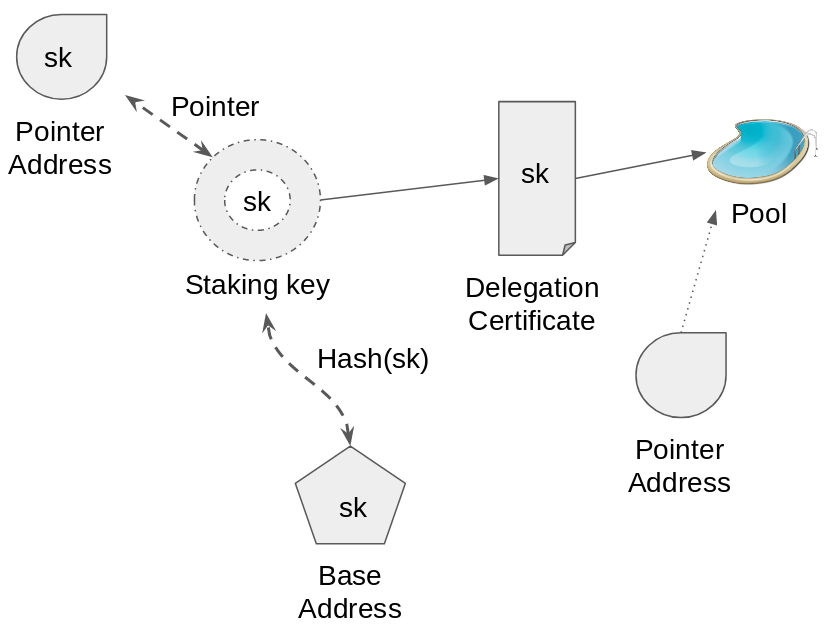
\includegraphics[width=0.6\columnwidth]{figures/delegation/delegation.png}
    \end{center}
    \caption{
        A representation of the delegation mechanism. Base pointers are linked
        to a key via a hash, whereas pointers may point to either a staking key
        or a pool directly.
    }
    \label{fig:delegation}
\end{figure}

Delegation certificates come in two forms, depending on how they are published.
\emph{Heavyweight} certificates are published on the ledger and are identified
by an \emph{index}, which represents the position of the certificate in the
ledger. The index is the tuple $ptr = (b, x, c)$, where $b$ relates to a block
in the ledger, $x$ represents a transaction in $b$, and $c$ identifies a
certificate in the metadata of $x$. Therefore, every pointer address contains
the index of the certificate to which it points. If an address $\addr$ points
to an invalid certificate, then $\addr$'s stake is not delegated.
\emph{Lightweight} certificates are not published by default, but instead
become public when their staking key participates in the PoS protocol.
Conflicts are resolved based on seniority. For instance, let $\stakingkeypair$
be a staking key which issues two certificates $\Sigma_1, \Sigma_2$. If they
are published on the ledger in that order, $\Sigma_2$ takes effect for all
addresses associated with $\stakingkeypair$. The metadata of a lightweight
certificate also contain a ``counter'', \ie an integer that breaks ties between
lightweight certificates; if two conflicting lightweight certificates are
presented, then whichever has the higher counter is accepted.

\paragraph{Certificate length}\label{sec:certificate-evaluation}
Let the curve of the ECDSA scheme be
\emph{secp256r1}~\cite{gupta2004ecc} and the hash function be \emph{SHA256}.
The staking pool registration certificate is the tuple $\Sigma =
(\stakingkeyverify, m, \sign)$. The public key size for $\stakingkeyverify$ (in
the compressed form) is $33$ bytes and the signature $\sign$ is $132$ bytes.
The metadata value $m$ depends on the implementation; for simplicity, we can
assume that it consists of only a hash, so its length is $32$ bytes. Therefore,
the staking pool certificate is $197$ bytes. The delegation certificate is the
tuple $\Sigma = (\stakingkeyverify_s, \stakingkeyverify_{delegate}, m, \sign)$.
As before, the public keys $\stakingkeyverify_s, \stakingkeyverify_{delegate}$
are $33$ bytes each, whereas the signature $\sign$ is $132$ bytes. The metadata
$m$ contains the counter for the lightweight certificates; setting it to $1$
byte enables up to $256$ conflicting lightweight certificates. Therefore,
heavyweight and lightweight delegation certificates are $198$ and $199$ bytes
respectively.

\subsection{Protocol Participation}\label{sec:protocol-participation}

Participation in the PoS protocol consists of publishing specially-crafted,
protocol-related, signed messages. The address which is responsible for
participation at any given time is decided by the function $F_{PoS,player}$ and
its staking key is used to sign these messages. Here, we consider the typical
example of PoS participation, \emph{block generation}, \ie the act of extending
an existing chain with a newly-created block. For simplicity, a block is a
tuple $(\stakingkeyverify, m)$, where $\stakingkeypair$ is the staking key
which issues the block and $m$ is the block's contents, \ie the headers, the
tree of transactions, etc. As with delegation and stake pool registration, the
wallet obtains a signature for a new block via the staking interface of
$\FuncW$, while a verifier can similarly check it. However, whether a block is
valid for a given ledger, \ie whether a block can extend a chain, depends on
the protocol's chain validity rules. Notably, delegation affects these rules.
Next, we describe the validity rules in the presence of delegation, as well as
the rules that pertain to chain delegation, \ie the re-delegation of delegated
stake.

\paragraph{Block Validity}
For a chain $\chain$, the chosen address $\addr_{PoS}$ is associated with a
staking key $\stakingkeyverify_{PoS}$ and a candidate block $\block$ is signed
by a different staking key $\stakingkeypair$. The rules for deciding if
$\block$ is valid for $\chain$ are as follows:
\begin{itemize}
    \item if a delegation certificate for $\stakingkeyverify$ is published in
        $\chain$, $\block$ is invalid;
    \item else if a certificate that delegates from $\stakingkeyverify_{PoS}$
        to $\stakingkeyverify$ is published in $\chain$, $\block$ is valid;
    \item else if either no delegation for $\stakingkeyverify_{PoS}$ or a
        certificate that delegates from $\stakingkeyverify_{PoS}$ to
        $\stakingkeyverify_h$ is published in $\chain$ and $\block$ contains a
        lightweight certificate delegating from $\stakingkeyverify_h$ to
        $\stakingkeyverify$, $\block$ is valid;
    \item else $\block$ is invalid.
\end{itemize}

\paragraph{Chain Validity}
The empty chain $\chain = \epsilon$ is valid. Given a candidate chain $\chain =
\chain' || \block$, if $\chain'$ is valid and the block $\block$ is valid for
$\block$, then $\chain$ is valid.

\paragraph{Chain Decision}
Assume $\chain$ is the chain stored locally by the wallet and $\mathbb{C}$ is
the set of valid chains available on the network. The longest valid chain from
$\mathbb{C} \cup \{ \chain \}$ is chosen. In case of tie between two valid
chains $\chain_1$ and $\chain_2$, where $\head(\chain_1)$ and $\head(\chain_2)$
are signed by $(\stakingkeyverify_1, \stakingkeysign_1)$ and
$(\stakingkeyverify_2, \stakingkeysign_2)$ respectively, the following rules
apply:
\begin{itemize}
    \item if $\stakingkeyverify_1$ and $\stakingkeyverify_2$ are delegated via
        the heavyweight certificates $\Sigma_1$ and $\Sigma_2$, with indexes
        $idx_1$ and $idx_2$ respectively, $\chain_1$ is chosen if $idx_1 >
        idx_2$, otherwise $\chain_2$ is chosen;
    \item else if $\stakingkeyverify_1$ is delegated via the heavyweight
        certificate $\Sigma_1$ and $\stakingkeyverify_2$ is delegated via the
        \emph{lightweight} certificate $\Sigma_2$, $\chain_1$ is chosen;
    \item else if $\stakingkeyverify_1$ and $\stakingkeyverify_2$ are delegated
        via a combination of heavyweight and lightweight certificates
        $(\Sigma_{1,1}, \Sigma_{1,2})$ and $(\Sigma_{2,1}, \Sigma_{2,2})$
        respectively, then:
        \begin{itemize}
            \item if $\Sigma_{1,1}$ and $\Sigma_{2,1}$ have different indexes,
                then choose the one with the higher index;
            \item else if $\Sigma_{1,2}$ and $\Sigma_{2,2}$ have different
                counters, then choose the one with the higher counter;
            \item else choose the first observed on the network.
        \end{itemize}
\end{itemize}

\paragraph{Delegation Chains}\label{sec:chain_delegation}
Chain delegation is the ability of a staking key to re-delegate stake that has
been delegated to it. As described in Section~\ref{subsec:delegation}, the
metadata section of a delegation certificate defines the rules that pertain to
the certificate. One such rule relates to chain delegation. The metadata entry
for this property is a boolean value, ``allowChain'', which identifies whether
chain delegation is allowed for the applicable stake of the certificate.  For
example, let two certificates $\Sigma_0$ and  $\Sigma_1$, where $\Sigma_0$
delegates from a key $\stakingkeyverify_0$ to $\stakingkeyverify_2$ and sets
$\text{``allowChain''} = true$, whereas $\Sigma_1$ delegates from
$\stakingkeyverify_1$ to (the same key as before) $\stakingkeyverify_2$ and
sets $\text{``allowChain''} = false$. Suppose now that a third certificate
$\Sigma_3$ is published, delegating from $\stakingkeyverify_2$ to
$\stakingkeyverify_3$.  Although $\stakingkeyverify_3$ is eligible to
participate on behalf all addresses associated with $\stakingkeyverify_0$, it
cannot participate for those associated with $\stakingkeyverify_1$, since the
corresponding key is $\stakingkeyverify_2$ (as chain delegation is not
permitted for this key).  More concretely, a delegation chain is a list of
certificates $[\Sigma_1, \ldots, \Sigma_i]$ such that, for each certificate
$\Sigma_j, 1 < j \leq i$, it holds that $\Sigma_{j-1}[\stakingkeyverify_{d}] =
\Sigma_j[\stakingkeyverify_s]$  We say that $\stakingkeyverify$ is delegated
via a hain $[\Sigma_1, \ldots, \Sigma]$ if $\Sigma[\stakingkeyverify_{d}] =
\stakingkeyverify$.

\subsection{Security in the Presence of Stake Pools}\label{sec:stake-pooled-security}

In this section, first we analyze the security of stake pools \wrt the
underlying PoS protocol's security assumptions (cf.
Corollary~\ref{cor:stake-pooled}). Next, we discuss prominent hazards, namely
\emph{sybil} and \emph{replay} attacks.

\paragraph{Stake-pooled Security}
The security analysis of a PoS stake-pooled variant, \ie a PoS protocol with
stake pools, is based on the protocol's honest stake threshold assumption
$\tau$. This parameter identifies the minimum percentage of honest stake needed
for the protocol to be secure. It is typically set to $\frac{1}{2} + \epsilon$
or $\frac{2}{3} + \epsilon$, for some $\epsilon > 0$. For simplicity, we assume
that all stake is delegated to a total number of $P$ pools. Each pool possibly
controls a different amount of stake.  Let $P_h$ be the honest pools among $P$,
which control an aggregate $\rho_h$ percentage of the total stake.  When a
player delegates their stake, they effectively relinquish their staking rights.
Therefore, as Corollary~\ref{cor:stake-pooled} shows, the focus should be put
on the adversarial power over pools, rather than stake itself.  For example, if
the adversary delegates some stake to an honest pool, then this stake becomes
honest in the stake-pooled setting, as it is controlled by an honest leader.
Intuitively, the adversary compromises the stake-pooled variant's security by
corrupting an appropriate amount of pools, such that honestly-controlled stake
percentage is less than $\tau$. We stress that this does not imply that the
adversary is required to corrupt a large number of pools. For instance, if a
single pool controls $\rho_a \geq 1-\tau$ of the total stake, then the
adversary can compromise security by only corrupting this single, albeit large,
pool.

\begin{corollary}\label{cor:stake-pooled}
    The stake-pooled variant of a PoS protocol $\pi$ is secure if $\rho_h \geq
    \tau$, where $\rho_h$ is the percentage of the total stake controlled by
    pools which are managed by honest leaders and $\tau$ is the honest stake
    threshold assumption of $\pi$.
\end{corollary}

\paragraph{Sybil Attacks}
Using stake pools for the PoS protocol's execution, rather than the
stakeholders themselves, introduces the possibility of \emph{sybil
attacks}~\cite{douceur2002sybil}. Specifically, suppose that the adversary
creates a large number of stake pools. Honest players cannot immediately
identify whether a pool is adversarial, so these pools could appear legitimate
and (honest) users might be convinced to delegate to them, thus increasing the
adversarial stake ratio. This is an inherent problem to decentralized PoS
systems, as no form of external identification exists and an adversary can
easily create a large number of staking keys and registration certificates. A
potential countermeasure is to have pool leaders commit (some of) their own
stake to their pool.  In our setting, this method can be facilitated via an
extra field in the delegation certificate's metadata, which identifies the
leader's addresses and funds, which are committed to the pool. Evidently, as
long as these funds are locked in the corresponding addresses, a malicious
leader cannot use them for multiple pool commitments. While this does not
directly prevent a Sybil attack, it does force the attacker to commit some
stake to its pools, hence bounding its identity production capabilities.

\paragraph{Replay Attacks}
Another important consideration is replay protection. Replay attacks are
prominent in account-based ledgers, where an adversary may re-publish past
transaction. For instance, suppose Alice sends $x$ assets from her
address-account $\addr$ to Bob. After the payment is published, $\addr$
controls $y = z - x$ assets, $z$ being the funds that $\addr$ controlled before
Alice made the payment. In a replay scenario, Bob re-publishes this payment,
such that a further amount $x$ of funds is sent from Alice's account $\addr$ to
Bob's. The same vulnerability exists against the certificates of our scheme.
For instance, an attacker can re-publish a certificate to forcefully change a
user's delegation choice. To solve this issue, we employ an address
\emph{whitelist}. Specifically, each certificate defines the addresses allowed
to publish it. Naturally, this scheme assumes that the wallet knows these
addresses a priori.  Next, during certificate verification, a party checks
whether it is published in a transaction issued by a whitelisted address.  To
replay the certificate, the adversary would then need to obtain the private
payment key of one of the whitelisted addresses. Notably, our solution requires
no state to be maintained by the verifiers, as the information needed to
counter a replay attack, \ie the address whitelist, exists in the certificate
itself. Therefore, there is no the need to parse the entire ledger or maintain
extra local state, as is the case with counter-based replay protection
mechanisms~\cite{ethereumReplay}.

\subsection{Modes of Execution}\label{sec:wallet-modes}

Our final contribution is a set of modes of operation of a PoS wallet.

\paragraph{Regular}
This being most straightforward wallet deployment method, a regular wallet is
bootstrapped with a \emph{base} address $\addr_0$ and its stake is managed by a
key $\stakingkeypair$. After $\addr_0$ receives its first assets, the wallet
may perform staking actions by using $\stakingkeypair$. To perform staking on
its own, the wallet publishes a delegation certificate $\Sigma$ that delegates
to its own key $\stakingkeypair$. Subsequent addresses are pointer addresses to
$\Sigma$, so eventually all addresses are managed by the same staking key.
When the user wishes to delegate to a staking pool, identified by the key
$\stakingkeyverify_P$, the wallet simply publishes a certificate $\Sigma_d$
delegating from $\stakingkeyverify$ to $\stakingkeyverify_P$.

\paragraph{Offline with Cold Staking}
This wallet lives in an offline device, \eg on paper. It is rarely accessed for
payments, but regularly performs staking actions. It is bootstrapped similarly
to the regular wallet and, since its payment keys are stored offline, the
staking keys are managed as follows:
\begin{itemize}
    \item \emph{basic security}: the staking key $\stakingkeypair$, which
        manages all addresses, is online; in case $\stakingkeysign$ is
        compromised, the user accesses the payment keys and sends the funds to
        new addresses, controlled by a new staking key;
    \item \emph{enhanced security}: the wallet creates a certificate
        $\Sigma^\prime$, which delegates from $\stakingkeyverify$ to the
        ``hot'' key $\stakingkeyverify_h$; after $\Sigma^\prime$ is published,
        the user stores $\stakingkeypair$ offline and $(\stakingkeyverify_h,
        \stakingkeysign_h)$ online; in case $(\stakingkeyverify_h,
        \stakingkeysign_h)$ is compromised, $\stakingkeypair$ is used to
        delegate to a new ``hot'' key, without requiring access to the wallet's
        payment keys.
\end{itemize}

\paragraph{Enhanced Unlinkability of Addresses}
This wallet aims at a higher level of privacy, with each address managed by a
single staking key. Therefore, to change its delegation profile, the wallet
creates a certificate for each address. Additionally, it achieves different
security guarantees as follows:
\begin{itemize}
    \item \emph{online:} the wallet is online and creates only pointer
        addresses, which point to the stake pool's registration certificate; to
        re-delegate, it creates new pointer addresses and moves the funds from
        the old to the new addresses;
    \item \emph{offline:} the payment keys are stored offline, so the wallet
        creates base addresses, each managed by a unique staking key, and keeps
        the staking keys online; to re-delegate, it publishes a new certificate
        for each address.
\end{itemize}

\paragraph{The Stake Pool's Wallet}
A stake pool's wallet performs only staking actions, so its key
$(\stakingkeyverify_P, \stakingkeysign_P)$ is managed as follows:
\begin{itemize}
    \item \emph{basic security}: the key pair $(\stakingkeyverify_P, \stakingkeysign_P)$
        is stored online and is used directly for staking; in case of
        compromise, the wallet creates a new staking key while, for practical
        purposes, an alert mechanism should exist to notify the users to
        re-delegate their stake to the new key;
    \item \emph{enhanced security}: the wallet creates a lightweight
        certificate $\Sigma_l$, which delegates to a ``hot'' key
        $\stakingkeyverify_{Ph}$, and then stores $(\stakingkeyverify_P,
        \stakingkeysign_P)$ offline, while using $(\stakingkeyverify_{Ph}, \stakingkeysign_{Ph})$ and
        $\Sigma_l$ for staking; if $(\stakingkeyverify_{Ph}, \stakingkeysign_{Ph})$ is compromised, the
        wallet creates a new hot key $(\stakingkeyverify_{Ph}^\prime, \stakingkeysign_{Ph}^\prime)$ and a new
        lightweight certificate $\Sigma_l^\prime$, which delegates from
        $(\stakingkeyverify_{P}, \stakingkeysign_{P})$ to $\stakingkeyverify_{Ph}^\prime$ and includes a
        higher counter compared to $\Sigma_l$, using them for staking instead.
\end{itemize}
We note that, in particular, the stake pool's wallet is further explored in the
upcoming chapter on collective stake pools.

\section{Discussion}\label{sec:future}

Our framework offers a range of choices for embedding information in PoS
addresses, as well as enabling multiple address types.  The former allows the
addition of \emph{metadata} into the addresses, including keys for staking and
spending and \emph{device and account identification tags}. The latter gives
the ability to various players, \eg enterprises such as exchanges, to operate
using well-crafted, special-purpose addresses that are fit for special needs.
These features embrace a wide range of the desiderata outlined in
Section~\ref{sec:desiderata-delegation}. \emph{Address Non-Malleability} is addressed
during the address generation phase, described in detail in
Section~\ref{subsec:malleability_predicate}. Moreover, the two types of keys,
for payment and staking, cover the need for \emph{Staking and Spending
Separation}, whereas \emph{Key Exposure Mitigation} is achieved by providing
the flexibility to issue new delegation certificates using the ``staking
action'' interface, in case the staking key of the delegate is compromised.
\emph{Address Uniqueness} is addressed by the checks that the functionality
performs upon receiving a possible address from the adversary. Additionally,
the flexibility on defining attributes allows for \emph{Multiple Devices
Support} and \emph{Address Recovery}, by constructing special tags that are
embedded in the address. Furthermore, \emph{Delegation Verification} is
possible by obtaining the delegation certificates that pertain to its staking
key. Another advantage of this design is the \emph{Cost Effectiveness} of the
delegation mechanism, assigning and changing a delegate at the cost of only one
transaction. The delegation mechanism also allows a party to prove that it has
the right to append the ledger, although possibly restricting \emph{Chain
Delegation}. Finally, our framework enables a smooth \emph{bootstrapping}
delegation process, by allowing an initial delegation assignment phase which
depends on the implementation details of the ledger.

Notably, our desiderata revolve primarily around key management and address
generation. Therefore, we don't capture network reliability or availability
requirements, but rather assume an abstract ledger model, which satisfies
persistence and liveness in a synchronous setting. This allows us to focus on
address and signature generation, while treating the other components of the
system as black boxes, which presumably satisfy the required properties. This
is evident in Section~\ref{sec:delegation-transaction}, which assumes a generic
ledger model, abstracted as a set of variables and algorithms. Nonetheless, a
more rigorous analysis on the incorporation of our wallet core in a complete
wallet is an important next step. Such treatment could formally capture
security on all layers, \ie key management, consensus, network, \etc A possible
path towards this goal could propose a variant of $\FuncW$ with key-evolving
signatures, which would replace $\mc{F}_{\mathsf{KES}}$ in a protocol like
Ouroboros Praos~\cite{EC:DGKR18}, followed by a rigorous proof of security of
this consensus protocol variant.


\chapter{
    Collective Stake Pools
}\label{chap:collective-pools}

Both PoW and PoS ledgers are economies of scale, favoring parties with large
amounts of participating power. One reason is poorly-designed incentives,
resulting in disproportionate power
accumulation~\cite{karakostas2019cryptocurrency,FC:FKORVW19}. Another is
temporal discounting, \ie the tendency to disfavor rare or delayed
rewards~\cite{Reed2011}. Specifically, in Bitcoin, a party is rewarded for
every block it produces, so parties with insignificant amounts of power are
rarely rewarded. In contrast, accumulating the power of multiple small parties
in ``pools'' yields a steadier reward.

As a result, these systems often see the formation of collaborative entities of
participants. In PoW systems, this takes the form of mining
pools.\footnote{$86$\% of Bitcoin's hashing power and $83$\% of Ethereum's
hashing power are controlled by $5$ entities each.
(\url{https://miningpools.com}; May 2021)} Similarly, PoS systems often opt for
stake pools, \ie collaborative entities comprising of multiple stakeholders,
which allow a party to earn rewards more regularly, compared to participating
on an individual basis.  Particularly in PoS, delegation to stake pools is
often preferred over ``pure'' PoS, where parties act independently, as the
ledger's performance and security is often better under fewer participants. For
instance, PoS systems require participants to be constantly online, since
abstaining is a security hazard; this requirement is more easily guaranteed
within a small set of dedicated delegates.

However, a major drawback of existing stake pool designs, including our scheme
of Chapter~\ref{chap:delegation}, is that they are typically managed by a
single party, \ie the pool operator. This party participates in consensus,
claims the rewards offered by the system, and then distributes them among the
pool's members (after subtracting a fee). However, the operator is a single
point of failure. In this chapter, we extend the results of
Chapter~\ref{chap:delegation} by exploring a design which allows players to
jointly form a \emph{collective pool}, \ie a conclave. This design assumes no
single operator, minimizing excess fees, and trust and security concerns,
altogether. Collective stake pools also promote a more fair and decentralized
environment. In existing incentive
schemes~\cite{DBLP:conf/eurosp/BrunjesKKS20}, operators who can pledge large
amounts of stake to the pool are preferred. Consequently, the system favors a
few major pool operators and, in the long run, its wealth is concentrated
around them, resulting in a ``rich get richer'' situation. Although this
problem is inherent in all decentralized financial
systems~\cite{karakostas2019cryptocurrency}, a well-designed collective pool
may offset the stakeholder imbalance and slightly decelerate this tendency.
Especially in PoS systems, a well-designed pool mechanism can prevent attacks
observed on PoW~\cite{FCW:JLGVM14,FC:WalCli14,FCW:LasJohGro15}.

\paragraph{Related Work}
In cryptographic literature, pools are mostly treated from an engineering
perspective. In PoW systems, SmartPool~\cite{USENIX:LVTS17} is a notable design
of a distributed mining pool for Ethereum, which, similar to our work, utilizes
smart contracts for reward distribution.  On the PoS domain,
Ouroboros~\cite{C:KRDO17} offers a brief description of how delegation can be
used within the protocol. This idea is expanded in~\cite{SCN:KarKiaLar20},
which provides a formal definition of PoS wallets and includes stake pool
formation method via certificates. However, the pool's management is again
centralized around the operator; our work extends this line of work by enabling
the formation of a collective pool. Another work, orthogonal to ours, by
Br{\"{u}}njes \etal~\cite{DBLP:conf/eurosp/BrunjesKKS20} considers the
incentives of distributing rewards among stake pools and aims to incentivize
the creation of a (pre-defined) number of pools. However, it assumes that the
pool operator commits part of their stake to make the pool more appealing, thus
favoring larger pool operators. Our work eases such wealth concentration
tendencies by enabling a collective pool to be equally competitive to a
centralized one.

\paragraph{Contributions}
The core contribution of this chapter is the ideal functionality $\Fpool$, a
simulation-based security definition of collective stake pools, which captures
the security properties of our collective pool scheme. We then describe
$\Ppool$, a distributed protocol executed by a set of $\totalParties$ parties
$\partyset$ which realizes $\Fpool$. A major consideration and performance
enhancement of our design is load balancing of transaction verification. Each
transaction is verified by a (deterministically elected) committee of parties,
whose size is a tradeoff between balancing workload, \ie not requiring each
party to verify every transaction, and reducing trust on the chosen
validator(s). We thus construct a distributed mempool, \ie a collectively
managed set of unpublished transactions, \st if a majority of the committee's
members are honest, transaction verification is secure.

\section{Desiderata}\label{sec:collective-pool-desiderata}

Our design assumes a group of stakeholders who jointly create a stake pool
without a single operator. Since large stakeholders typically form pools on
their own, our protocol concerns smaller stakeholders, who could otherwise not
participate directly. Therefore, our design could \eg be appealing to a group
of friends or colleagues, who aim for a more steady reward ratio without
relying on a third party. Importantly, it should operate in a trustless environment as,
unfortunately, even in these scenarios, trust is not
a given. Notably, our targeted audience is parties who wish to
actively participate, \ie always be online to perform the required consensus
actions; parties who wish to remain offline may instead opt for delegation
schemes~\cite{eosWhitepaper,SCN:KarKiaLar20}.

In the absence of a central party, the responsibility of running the pool is
shared among all pool's members, requiring some level of coordination which may
be cumbersome. For instance, if the protocol requires unanimous actions, a
single member could halt the pool's operation. To ensure good performance, the
pool should allow a subset (of a carefully chosen size) to act on behalf of the
whole group. The choice of such subsets depends on each party's ``weight'',
which is in proportion to their stake.  In summary, we have the following
initial assumptions, which form the basis for outlining our work's desiderata:

\begin{itemize}[noitemsep]
    \item \emph{small number of parties}: a collective pool is operated by a
        small group of players;

    \item \emph{small stake disparity}: the profiles of the collective pool's
        members are similar, \ie they contribute a similar amount of stake to
        the pool;

    \item \emph{stake proportion as ``weight''}: each party is assigned a
        weight for participating in the pool's actions, relative to their part
        of the pool's total stake.
\end{itemize}

Next, we provide an exhaustive list of basic requirements of a collective stake
pool. We note that an \emph{admissible party set} is a set of parties with
enough stake, \ie above a threshold of the total pool's stake which is agreed
upon during the pool's initialization. To the extent that some desiderata are
conflicting, our design will aim to satisfy as many requirements as possible:
\begin{itemize}[noitemsep]
    \item \emph{Proportional Rewards}: the claim of each member on the
        entire pool's protocol rewards should be proportional to
        their individual contribution.

    \item \emph{Joint Control of Rewards}: the members of a pool should
        jointly control the access to its funds.

    \item \emph{Unilateral Reward Withdrawal}: at any point in time, a
        stakeholder should be able to claim their reward,
        accumulated up to that point, without necessarily interacting with
        other members of the pool.

    \item \emph{Permissioned Access}: new users can join the pool following
        agreement by an admissible set of pool members.

    \item \emph{Robustness against Aborting}: the pool should not fail to
        participate in consensus, unless an admissible set of members aborts or
        is corrupted.

    \item \emph{Public Verifiability}: stake pool formation and operation
        should be publicly verifiable (\st consensus could take into account
        the aggregate pool's stake).

    \item \emph{Stake Reallocation}: users should freely change their
        personal stake allocated to the pool, without interacting with other
        members of the pool.

    \item \emph{Parameter Updates}: an admissible set of parties should be
        able to update the stake pool's parameters.

    \item \emph{Force Removal}: an admissible set of parties should be able
        to remove a member from the pool.

    \item \emph{Pool Closing}: an admissible set of parties should be able to
        permanently close the stake pool.

    \item \emph{Prevention of Double Stake Allocation}: a party should not
        simultaneously commit the same stake to two different stake pools.
\end{itemize}

\section{Execution Model}\label{sec:execution-model}

In our setting, the ledger's maintainers are the stake pools. An adversary can
break the ledger's properties by corrupting a set of stake pools which are
allocated a majority of the total stake. Consequently, since we assume that the
majority of stake is owned by honest stakeholders, the adversary needs to
corrupt at least one pool to which honest players delegate. Especially in the
collective setting, the adversary may control a subset of the pool's members,
although not a majority of them. Therefore, our work considers adversaries who
attempt to violate the security of a collectively-owned stake pool while
controlling a minority of its members. Security violations include producing
invalid blocks or transactions, as well as abstaining from join the consensus
protocol.

In terms of message delivery, we assume a synchronous network.  As such, the
adversary may delay messages up to an upper bound. This assumption will prove
particularly useful in the implementation of the collective pool protocol,
during which participants employ consensus and broadcast algorithms. We note
that, although this assumption is realizable in a setting where parties are
well-connected, it does not cover possible real-world threats, such as eclipse
attacks. Nonetheless, exploring variations of the collective pool functionality
and protocol designs over semi-synchronous or asynchronous networks presents an
interesting problem, which would offer a more robust implementation.

\subsection{Weighted Threshold Digital Signatures}\label{sec:thold-sign}

In a weighted threshold digital signature
scheme~\cite{morillo1999weighted,Shamir79}, each party $\party$ is associated
with a (integer) weight $\wfunc[\party] \geq 0$, where $\wfunc$ is a mapping of
players to weights. A signature can be produced by any set of keys, the
aggregate weight of which is above the defined threshold. The weighted
threshold signature scheme (Definition~\ref{def:thresh-sig}) is constructed by
combining a digital signature scheme (Definition~\ref{def:digsign}) with a
weighted threshold secret sharing scheme (Definition~\ref{def:thresh-ss}).
Additionally, standard threshold signatures is a special case of the weighted
variant, with $\wfunc[\party] = 1$ for every party $\party$.

\begin{definition}[Weighted Threshold Secret Sharing]\label{def:thresh-ss}
    A $(\thold, \totalParties, \wfunc)$-threshold secret sharing of a secret
    $x$ consists of $n$ shares $x_1, \dots, x_{\totalParties}$, each associated
    with a weight $\weight_1, \dots, \weight_\totalParties$, such that an
    efficient algorithm exists, that takes as input a set of shares
    $\tholdset$, with $\sum_{i \in \tholdset} \weight_i > \thold$, and
    outputs the secret value $x$. Any set of shares $\tholdset$
    with $\sum_{i \in \tholdset} \weight_i \leq \thold$ cannot obtain any
    information about the secret $x$.
\end{definition}

\begin{definition}[Weighted Threshold Signature]\label{def:thresh-sig}
    Given a signature scheme $\sigscheme$, a $(\thold, \totalParties,
    \wfunc)$-threshold signature scheme $\threshsigscheme = \langle \threshkeygen, \threshsign, \threshver \rangle$, given $\totalParties$ parties
    $\p_1, \dots, \p_{\totalParties} \in \parties$, is defined as:
    \begin{itemize}
        \item $\threshkeygen(1^\secparam, \wfunc) \rightarrow (\keyverify,
            \keysign_1, \dots, \keysign_n)$:
            given the security parameter $\secparam$, outputs a public key
            $\keyverify$ and a list of private keys $\keyset = [\keysign_{1}, \dots,
            \keysign_{\totalParties}]$ which form a $(\thold, \totalParties,
            \wfunc)$-threshold secret sharing of $\keysign$; the pair
            $(\keyverify, \keysign)$ has the same distribution as the keys
            output by $\algokeygen$ of Definition~\ref{def:digsign};

        \item $\threshsign(\mesg, \tholdset) \rightarrow \signature$:
            given a message $\mesg$ and a set of private keys
            $\tholdset$, $\tholdset \subseteq \keyset$, outputs a
            signature $\signature$;

        \item $\threshver(\mesg, \keyverify, \signature) \rightarrow \{0,1\}$: a
            deterministic algorithm that, given a message $\mesg$, a public key
            $\keyverify$, and a signature $\signature$ outputs $1$ if a
            signature is valid \wrt message $m$ and verification key
            $\keyverify$ (resp. $0$ if the signature is invalid).
    \end{itemize}

    A $(\thold, \totalParties, \wfunc)$-threshold signature scheme
    $\threshsigscheme$ is $\eufcma$ if it presents the properties of
    Definition~\ref{def:digsign} and the following:

    {\bf Threshold Completeness:} For any message $\mesg$, it holds:
    \begin{align}
        \Pr[(\keyverify, \keyset) \leftarrow \threshkeygen(1^\secparam, \wfunc), \signature \leftarrow \threshsign(\mesg, \tholdset),  \nonumber \\
        \sum_{k \in \tholdset} \weight_k > \thold: 0 \leftarrow \algover(\mesg, \signature, \keyverify)]
        \leq \negl(\secparam) \nonumber
    \end{align}
    and
    \begin{align}
        \Pr[(\keyverify, \keyset) \leftarrow \threshkeygen(1^\secparam, \wfunc), \signature \leftarrow \threshsign(\mesg, \tholdset),  \nonumber \\
        \sum_{k \in \tholdset} \weight_k \leq \thold: 1 \leftarrow \algover(\mesg, \signature, \keyverify)]
        \leq \negl(\secparam) \nonumber
    \end{align}
    where all the probabilities are computed over the random coins of the
    key generation and sign algorithms.
\end{definition}

\subsection{Transactions, Blocks, and the Global Ledger}\label{sec:global-ledger}
Our protocol utilizes two features of the Kachina~\cite{kachina} framework: i)
the formalization of the ledger and ii) smart contracts.

\paragraph{The Simple Ledger Functionality}
Our collective pool protocol interacts with a ledger functionality in a hybrid
execution.  One option is the formalization of Bitcoin's ledger from~\cite{C:BMTZ17}.
However, this functionality is local, while we would prefer a global
functionality, following the Global UC Framework~\cite{TCC:CDPW07}, hence we
will use the $\Gledger$ functionality from Kachina~\cite{kachina}. The
functionality is available in Figure~\ref{fig:gledger}, where $\prec$ defines
the prefix operation, \ie $\contractstate\prec\contractstate^\prime$ means the
state $\contractstate$ is included in $\contractstate^\prime$, and, for
readability and consistency purposes, we rename \emph{transaction} ($\tau$) to
\emph{block} ($b$).

\myhalfbox{Global Ledger Functionality $\Gledger$}{white!40}{white!10}{
    The functionality keeps a state $\contractstate$ and a mapping $M$ of parties to
    states, both initially empty.

    \begin{itemize}
        \item When receiving a message $(\mathsf{SUBMIT}, b)$ from a party
            $p$, query $\adversary$ with $(\mathsf{BLOCK}, b)$.

        \item When receiving a message $\mathsf{READ}$ from a party $p$,
            return $M(p)$; if $p$ is $\adversary$, it returns $\contractstate$.

        \item When receiving a message $(\mathsf{EXTEND}, \contractstate^\prime)$ from
            $\adversary$, set $\contractstate \leftarrow \contractstate || \contractstate'$.

        \item When receiving a message $(\mathsf{ADVANCE}, p, \contractstate^\prime)$ from
            $\adversary$, if $M(p) \prec \contractstate^\prime \prec \contractstate$ then set $M(p)
            \leftarrow \contractstate^\prime$.
    \end{itemize}

}{\label{fig:gledger} The Simple Global Ledger Ideal Functionality.}

The $\Gledger$ Functionality is generic enough to abstract transactions and
blocks, focusing on the ledger's properties. However, in our setting we need to
define these objects, in order to better formulate a real-world blockchain.

In this chapter, a transaction is $\tx = \langle \addr_s,
\addr_r, v, f \rangle$, where
\begin{inparaenum}[i)]
    \item $\addr_s, \addr_r \in \{0, 1\}^*$ are the sender's and receiver's
        addresses respectively,
    \item $v \in \mathbb{R}$ is the value transferred from $\addr_s$ to
        $\addr_r$, and
    \item $f \in \mathbb{R}$ is the fees of the transaction.
\end{inparaenum}
A block consists of an ordered list of transactions. To organize transaction in
blocks, we assume a function $\blockify$ which, given a set of transactions and
a chain, returns a block which can extend the chain, \ie satisfies the validity
requirements of the system.

\paragraph{Reward Management via Smart Contracts}
We also employ the formal model of smart contracts from~\cite{kachina}. This
model considers smart contracts from a privacy-preserving perspective.
However, it also provides a UC definition of standard smart contracts,
consisting of the universal machine $\mc{U}$, which acts as the oracle over the
ledger's state, and the \emph{core} contract $\Gamma$, as illustrated by
Figure~\ref{fig:rewardFunc} adapted to our stake pool design. In our setting,
the latter relates directly to the management of the rewards for the members of
the pool, and therefore it is presented as an auxiliary (reward) functionality
$\rewardFunc$ in Section~\ref{sec:management}.

\paragraph{Delegation and Stake Pools}\label{sec:delegation}
We utilize the UC Model for delegated PoS systems, as presented in
Chapter~\ref{chap:delegation}. This framework partially fulfills our earlier
desiderata. In particular, \emph{Prevention of Double Stake Allocation} and
\emph{Public Verifiabilitty} are addressed by the certificate-based
registration and revocation mechanisms.  However, the remaining items do not
seem immediately solved without further assumptions. For instance, if the
members have the same proportion of shares, a standard threshold signature
scheme could address more of our desiderata, \eg \emph{Offline and Online
Participation}, \emph{Pool Proportional Rewards}, \emph{Joint Control of
Rewards}, and \emph{Robustness against Aborting}.  Following, reconfiguration
of the pool is accomplished by regenerating the registration certificate and
the pool's threshold key. Other desiderata can be approached in a similar
fashion. Thus, our idea is to generalize the access structure of an efficient
threshold signature scheme to add ``weight'' capabilities, such that the
weights capture the pledged stake distribution among the pool's members.

\section{UC Weighted Threshold Signature}\label{sec:uc-weighted-tss}

In this section, we present the weighted threshold signature ideal functionality
$\Fweight$ (Figure~\ref{fig:Fweight}). This functionality is used by the
Collective Pool Protocol $\Ppool$ to collectively sign certificates and new
blocks. The functionality $\Fweight$ is inspired by Almansa
\etal~\cite{EC:AlmDamNie06}, which is in turn inspired by
Canetti~\cite{EPRINT:Canetti03}. However, unlike Almansa \etal and similar to
Canetti, during signature verification we consider the case of a corrupted
signer, \ie a set of parties such that the majority (of weights) is corrupted.

$\Fweight$ interacts with a set of $\totalParties$ parties. Each party
$\party_i$ is associated with an integer $\weight_i$, \ie its weight.
$\Fweight$ also keeps the following, initially empty, tables:
\begin{inparaenum}[i)]
    \item $\mathsf{pubkeys}$: tuples $\langle sid, \pubkey \rangle$ of $sid$
        and a public key $\pubkey$;
    \item $\mathsf{sigs}$: tuples $(m, \signature, \pubkey, f)$ of message
        $m$, a signature $\signature$, a public key $\pubkey$, and a
        verification bit $f$.
\end{inparaenum}
The mapping $\wfunc[\p] \rightarrow \weight_{\p}$ denotes the weight of a party
$\p$, while the term $\wfunc$ also denotes the set of keys the participating
parties.

\myhalfbox{Weighted Threshold Signature Functionality $\Fweight$}{white!40}{white!10}{
    Each message is associated with $sid = \langle \parties,
    \wfunc, \thold, sid' \rangle$, where $\parties$ is the set of parties,
    $\wfunc$ is a mapping of parties to weights, $\thold$ is the collective
    signature weight threshold, and $sid'$ is a unique identifier.

    \noindent{\bf Key Generation:}
        Upon receiving $\msg{KeyGen}{}$ from every honest party $\party \in
        \parties$, send $\msg{KeyGen}{\party}$ to $\iadv$. Upon receiving a
        response $\msg{KeyGen}{\threshpubkey}$ from $\iadv$, record $\langle
        sid, \threshpubkey \rangle$ to $\mathsf{pubkeys}$ and send
        $\msg{KeyGen}{\threshpubkey}$ to every party in $\parties$. Following,
        all messages that do not contain the established $sid$ are ignored.

    \noindent{\bf Signature Generation:}
        Upon receiving $\msg{Sign}{m}$ from a party $\p$, forward it to
        $\iadv$. After a subset of parties $\parties' \subseteq \parties$ has
        submitted a $\mathsf{Sign}$ message for the same $m$, and upon
        receiving $\msg{Sign}{m, \signature}$ from $\iadv$, check that
        $\sum_{\p \in \parties'} \wfunc[\p] > \thold$ (\emph{Note: This
        condition guarantees threshold completeness.}) Next, if $(m,
        \signature, \threshpubkey, 0) \not \in \mathsf{sigs}$ (for the key
        $\threshpubkey$ that corresponds to $sid$ in $\mathsf{pubkeys}$),
        record $(m, \signature, \threshpubkey, 1)$ to $\mathsf{sigs}$ and reply
        with $\msg{Sign}{m, \signature}$.

    \noindent{\bf Signature Verification:}
        Upon receiving $\msg{Verify}{m, \signature, \threshpubkey'}$ from
        $\party$, forward it to $\iadv$. Upon receiving $\msg{Verified}{m,
        \signature, \phi}$ from $\iadv$, set $f$ as next:
        \begin{enumerate}
            \item If $\threshpubkey' = \threshpubkey$ and $(m, \signature,
                \threshpubkey, 1) \in \mathsf{sigs}$, $f = 1$. (\emph{This
                guarantees completeness.})
            \item Else, if $\threshpubkey' = \threshpubkey$, the aggregate
                weight of the corrupted parties in $\parties$ is strictly less
                than $\thold$, and $(m, \signature, \threshpubkey, 1) \not \in
                \mathsf{sigs}$, $f = 0$ and record $(m, \signature,
                \threshpubkey, 0)$ to $\mathsf{sigs}$. (\emph{This guarantees
                unforgeability, if the aggregate weight of the corrupted
                parties is below the threshold.})
            \item Else, if $(m, \signature, \threshpubkey', b) \in
                \mathsf{sigs}$, $f = b$. (\emph{This
                guarantees consistency.})
            \item Else, $f = \phi$ and record $(m, \signature,
                \threshpubkey', f)$ to $\mathsf{sigs}$.
        \end{enumerate}
        Finally, send $\msg{Verified}{m, \signature, \threshpubkey', f}$ to
        $\party$.

}{\label{fig:Fweight} Weighted Threshold Signature Ideal Functionality}

As highlighted in the definition, \emph{completeness, consistency}, and
\emph{unforgeability} are enforced upon verification, whereas \emph{threshold
completeness} is enforced upon signature generation. Hence, it should be
infeasible to issue a signature unless using keys with enough weight, \ie above
the threshold $\thold$.

\section{The Collective Stake Pool}\label{sec:stake-pool}

Our analysis is based on the UC Framework, following Canetti's formulation of
the ``real world''~\cite{EPRINT:Canetti00}. Specifically, we define the
collective pool ideal functionality $\Fpool$, which distills the required
(operational and security) properties; for readability, $\Fpool$ is divided in
two parts, \emph{management} and \emph{consensus participation}. The ideal
functionality is realized --- in the ``real world'' --- by the distributed
protocol $\Ppool$, which employs various established cryptographic primitives,
and, therefore, $\Ppool$ can described with auxiliary functionalities.
Before proceeding with the functionality's definition, we first describe the
hybrid execution of $\Ppool$ and its building blocks.

\subsection{Hybrid Protocol Execution}\label{sec:execution}

The protocol $\Ppool$ is performed by $n$ parties, where each party $\p_i$
holds two pairs of keys: $(\keyverify_{\p_{i}}, \keysign_{\p_{i}})$ for issuing
transactions, and $(\keyverify_{s_{i}}, \keysign_{s_{i}})$ for staking
operations, \eg issuing delegation certificates (cf.~\cite{SCN:KarKiaLar20}). The
public key $\keyverify_{i}$ is also used to generate an address $\addr_{i}$.
Each pool member $\p_i$ pledges the funds of an address $\addr_{i}$ (which it
owns) to the pool. These funds are the player's stake in the pool and form
the player's weight in the weight distribution mapping $\wfunc$.

We assume the members' stake, \ie their weight $\weight_{i}$ in the pool, is
public. Therefore, the weight distribution mapping $\wfunc$ is also public.
Furthermore, each member of the pool has its own signature key, and can issue
standard signatures through a standard signature scheme.  A
weighted version for a threshold signature scheme follows by having each party
holding as many shares, of the original threshold scheme, as its weight. This
approach has the extra advantage that security guarantees of the original
scheme are carried straightforwardly into the weighted version.

Additionally, our construction relies on the consensus sub-protocol $\Pconsensus$
to validate a transaction by the elected committee.
Specifically, the collective stake pool protocol is
parameterized by:
\begin{inparaenum}[i)]
    \item the validation predicate $\algovalidate$,
    \item the permutation algorithm $\permutationAlgo$, and
    \item a consensus sub-protocol $\Pconsensus$.
\end{inparaenum}

Our (modular) protocol is described in a hybrid world with auxiliary
functionalities for established primitives. The functionality
$\Fbroad$~\cite{EC:HirZik10} provides a reliable broadcast channel to all parties;
$\Fcore$ (cf. Chapter~\ref{chap:delegation}) enables delegation to the pool;
$\Fweight$ (cf. Section~\ref{sec:uc-weighted-tss}) enables weighted threshold
signature operations; the Smart Contract Functionality $\rewardFunc$ realizes
the reward distribution mechanism; $\Gledger$ is a global Ledger
Functionality~\cite{kachina}. Finally, we use $\hybpool$ to denote the $\{
    \Gledger, \Fbroad, \Fcore, \Fweight, \rewardFunc \}$-hybrid execution of
$\Ppool$ in the (global) UC Framework.

\subsection{Part 1: Stake Pool Management}\label{sec:management}

The functionality's first part (Figure~\ref{fig:Fpool-1}) includes all
operations that are not consensus-oriented. First, establishing a stake pool
consists of two parts, defined as corresponding interfaces in the ideal
functionality. The pool's members gather and jointly decide to create a staking
pool; they contact each other, \eg via off-chain direct channels, agree on the
pool's parameters, and generate its key. Importantly, the participants are
aware of the total number of participants in the pool, as well as their
weights. Then, the members of the pool perform a setup protocol and register
the new pool via a registration certificate, which is signed by the pool's key
and published on the ledger. Following, the pool receives rewards for
participating in the consensus protocol. The rewards are managed by a smart
contract and, at any point, each each party can withdraw their part, which is
proportional to the internal stake distribution. Finally, to close the pool,
the members sign and publish a revocation certificate.

In more detail, the functionality $\Fpool$ interacts with $\totalParties$
parties $\party_1, \dots, \party_\totalParties$ and is parameterized by:
\begin{itemize}
    \item the validation predicate $\algovalidate(\cdot, \cdot)$ which, given a
        transaction $\tx$ and a chain $\chain$, defines whether $\tx$ can be
        appended to $\chain$ (as part of a block);
    \item the algorithm $\blockify$ which, given a set of transactions,
        serializes them (deterministically) in a block;
    \item the probability $\prob^{\subselectionParam, \adversarialParties,
        \totalParties}$ that the elected committee, responsible for a
        transaction's verification, is corrupted, dependent on the subselection
        parameter $\subselectionParam$ and the number of corrupted parties
        $\adversarialParties$ out of $\totalParties$ total parties.
\end{itemize}

It also keeps the following, initially empty, variables:
\begin{inparaenum}[i)]
    \item the signature threshold $\thold$;
    \item the public key $\threshpubkey_{pool}$;
    \item the reward address $\addr_{reward}$;
    \item the set of valid and unpublished transactions $\mathsf{mempool}$;
    \item a mapping of parties to weights $\members$;
    \item a table of signatures $\mathsf{sigs}$.
\end{inparaenum}

\paragraph{Gathering and Registration}
The first step in creating a pool is the gathering of parties, in order to
collectively create the pool's public key $\threshpubkey_{pool}$. Following,
the parties create and publish on the ledger the registration certificate
$\cert_{reg}$, which contains the following:
\begin{itemize}[noitemsep]
    \item $\wfunc$: a mapping identifying each member's weight;
    \item $\addr_{reward}$: the address which accumulates the pool's rewards;
    \item $\threshpubkey_{pool}$: the pool's threshold public key;
    \item $\threshsig_{pool}$: the signature of $\langle \wfunc, \addr_{reward}
        \rangle$ created by $\threshpubkey_{pool}$.
\end{itemize}

\paragraph{Reward Withdrawal}
During the life cycle of the pool, a member may want to withdraw the rewards
received up to that point. As per the desiderata of
Section~\ref{sec:collective-pool-desiderata}, any party should be able to do so, without the
explicit permission of the other pool's members. Additionally, the rewards that
each party receives should be proportional to its stake, \ie its weight within
the collective pool. Reward withdrawal is implemented as the smart contract
functionality $\rewardFunc$. The contract is initialized with the weight
distribution of the pool's members and each member's public key. We assume that
the contract is associated with an address and can receive funds,
similar to real-world smart contract systems like
Ethereum~\cite{wood2014ethereum}. The state transition functionality
$\rewardFunc$ is defined in Figure~\ref{fig:rewardFunc} (following the ledger
formalization of Section~\ref{sec:global-ledger}).

\myhalfbox{Reward Smart Contract Functionality $\rewardFunc$}{white!40}{white!10}{
    $\rewardFunc$ maintains a mapping $\wfunc$, of parties to weights,
    and a variable $b$.

    \noindent{\bf Initialization:}
        Upon receiving $\msg{init}{\wfunc^\prime}$, forward it to $\iadv$. Upon receiving
        a response $\msg{init-ok}{\addr_{sc}}$, set $\wfunc \leftarrow \wfunc^\prime$ and
        return $\msg{init-ok}{\addr_{sc}}$.

    \noindent{\bf Balance Update:}
        On receiving $\msg{transaction}{\tx}$ from $\mc{U}$, such that $\tx =
        \langle \addr_s, \addr_r, v, f \rangle $, if $\addr_s = \addr_{sc}$ set
        $b := b - v$, else if $\addr_r = \addr_{sc}$ set $b := b + v$.

    \noindent{\bf Withdrawal:}
        Upon receiving $\msg{withdraw}{\addr, f}$ from the party $\p$, set $r =
        \frac{\weight_p}{\sum_{p^\prime \in \wfunc} \weight_{p^\prime}} \cdot b$ and return
        $\msg{transaction}{\langle \addr_{sc}, \addr, r, f \rangle}$.

}{\label{fig:rewardFunc} The pool's Reward Smart Contract Functionality.}

\paragraph{Closing}
Eventually, the members halt the operation of the pool. In order to do so, they
revoke the pool's registration by jointly producing a revocation certificate
$\cert_{rev}$. The certificate is relatively simple, containing a timestamp $x$
announcing the end of the pool and signed by the pool's public key
$\threshpubkey_{pool}$.

The first part of our functionality definition is given by
Figure~\ref{fig:Fpool-1}, whereas the management routines, \ie the first part
of the description, of our protocol construction is given by
Figure~\ref{fig:Ppool-1}.

\myhalfbox{Collective Pool Functionality $\Fpool^{\thold,\wfunc}$ (first part)}{white!40}{white!10}{
    \noindent{\bf Gathering:}
        Upon receiving $\msg{gather}{}$ from $\p$, forward it to $\iadv$. After
        every party $\p_i, i \in [1, \totalParties]$ has submitted
        $\mathsf{gather}$, upon receiving from $\iadv$
        $\msg{gather-ok}{\threshpubkey_{pool}}$, store $\thold$ and
        $\threshpubkey_{pool}$, add all party-weight pairs $(\p_{i}, \wfunc_i)$
        to $\members$, and reply with
        $\msg{gather-ok}{\threshpubkey_{pool}}$ to all parties.

    \noindent{\bf Pool Registration:}
        Upon receiving $\msg{register}{\members}$ from $\p$, forward it
        to $\iadv$. After all parties $\p_i, i \in [1, \totalParties]$ have
        submitted $\mathsf{register}$, upon receiving from $\iadv$
        $\msg{register-ok}{\addr_{reward}, \threshsig_{pool}}$, set $\cert_{reg}
        = \langle (\members, \addr_{reward}, \threshpubkey_{pool},
        \threshsig_{pool}) \rangle$. Then check if $\forall (m, \sigma, b') \in
        \mathsf{sigs}: \sigma \neq \threshsig_{pool}, (\cert_{reg},
        \threshsig_{pool}, 0) \not \in \mathsf{sigs}$; if the checks hold,
        insert $(\cert_{reg}, \threshsig_{pool}, 1)$ to $\mathsf{sigs}$.
        Finally, store $\addr_{reward}$ and reply with
        $\msg{register-ok}{\cert_{reg}}$.

    \noindent{\bf Reward Withdrawal:}
        Upon receiving the message $\msg{withdraw}{\addr, f}$ from $\p_{i}$,
        forward it to $\iadv$. Then, compute $\reward =
        \frac{\weight_{\p_i}}{\sum_{j = 1}^{\totalParties} \weight_{\p_j}}
        \cdot \reward_{pool}$, where $\reward_{pool}$ is the funds of address
        $\addr_{sc}$ as defined in $\Gledger$. Finally, return
        $\msg{transaction}{\langle \addr_{sc}, \addr, \reward, f \rangle}$.

    \noindent{\bf Closing:}
        Upon receiving $\msg{close}{x}$ from $\p$, forward it to $\iadv$. After
        a set of parties $\tholdset$ has submitted $\mathsf{close}$ for the
        same $x$, if $\sum_{\p \in \tholdset} \weight_{\p} > \thold$, upon
        receiving $\msg{close-ok}{\threshsig_{pool}}$ from $\iadv$, check if
        $\forall (m, \sigma, b') \in \mathsf{sigs}: \sigma \neq
        \threshsig_{pool}, (x, \threshsig_{pool}, 0) \not \in \mathsf{sigs}$;
        if the checks hold, insert $(x, \threshsig_{pool}, 1)$ to
        $\mathsf{sigs}$. Finally, return to all parties
        $\msg{close-ok}{\cert_{rev}}$, with $\cert_{rev} = \langle x,
        \threshsig_{pool} \rangle$.

}{\label{fig:Fpool-1} The first part of the Collective Pool Functionality, parameterized with threshold $\thold$ and weight mapping $\wfunc$, refers to the creation and management of the pool (the second part is given by Figure~\ref{fig:Fpool-2}).}

\myhalfbox{Collective Pool Protocol $\Ppool^{\thold,\wfunc}$ (first part)}{white!40}{white!10}{
    \noindent{\bf Gathering:}
        Upon receiving $\msg{gather}{}$, send $\msg{KeyGen}{}$ to $\Fweight$,
        with $sid$ containing the weight mapping $\wfunc$ and the threshold
        $\thold$. Upon receiving the reply
        $\msg{KeyGen}{\threshpubkey_{pool}}$, return
        $\msg{gather-ok}{\threshpubkey_{pool}}$.

    \noindent{\bf Pool Registration:}
        Upon receiving $\msg{register}{\members}$, send
        $\msg{init}{\members}$ to $\rewardFunc$ and wait for the reply
        $\msg{init-ok}{\addr_{reward}}$. Then, set $m = (\members,
        \addr_{reward})$ and send $\msg{Sign}{m}$ to $\Fweight$. Upon receiving a
        reply $\msg{Sign}{m, \threshsig_{pool}}$, return
        $\msg{register-ok}{\cert_{reg}}$, where $\cert_{reg} = \langle
        (\members, \addr_{reward}, \threshpubkey_{pool},
        \threshsig_{pool}) \rangle$.

    \noindent{\bf Reward Withdrawal:}
        Upon receiving $\msg{withdraw}{\addr, f}$, forward it to $\rewardFunc$.
        Upon receiving a response $\msg{transaction}{\langle \addr_{sc}, \addr,
        r, f \rangle}$ return it.

    \noindent{\bf Closing:}
        Upon receiving $\msg{close}{x}$, send $\msg{Sign}{x}$ to $\Fweight$.
        Upon receiving a reply $\msg{Sign}{x, \threshsig_{pool}}$, return
        $\msg{close-ok}{\cert_{rev}}$ with $\cert_{rev} = \langle x,
        \threshsig_{pool} \rangle$.

}{\label{fig:Ppool-1} The first part of the Collective Pool Protocol, which describes the set of management operations (the second part is given by Figure~\ref{fig:Ppool-2}).}

\subsection{Part 2: Participation in Consensus}\label{sec:participation}

After a pool is set up, the functionality's second part
(Figure~\ref{fig:Fpool-2}) considers participation in the system, \ie
\emph{validating transactions} and \emph{issuing blocks}.
The pool members continuously monitor the network for new transactions, which
they collect, validate, and organize in a \emph{mempool}.  As mentioned in the
introduction, the pool members \emph{remain online} for the entirety of the
execution to perform the pool's operations. Specifically, when the pool is
elected to participate, the mempool's transactions are serialized and published
in a block. Under PoS, the pool participates proportionally to its
aggregated member and delegated stake.

To improve performance, we define a distributed mechanism for transaction
verification, \ie a \emph{distributed mempool}. Such load balancing mechanism
increases efficiency by requiring only a subset of the pool's members to verify
each transaction. Notably, this is in contrast to the standard practice of
Bitcoin mining pools, where the pool's operator decides the transactions to be
mined by its members; instead, our approach further reduces these trust
requirements.

To construct a distributed mempool, we consider a subselection mechanism to
identify the parties that verify each transaction. This mechanism should be:
\begin{inparaenum}[a)]
    \item \emph{non-interactive}
    \item \emph{deterministic},
    \item \emph{balanced}, \ie every party should be chosen with the same
        probability.
\end{inparaenum}
Subselection is secure if a majority of the elected committee is honest.
However, since the adversary may corrupt some pool members, this may not always
be the case. We model this uncertainty via the probability
$\prob^{\subselectionParam, \adversarialParties, \totalParties}$, which depends
on the size of the committee and the power of the adversary among the pool's
members.

A straightforward way to implement subselection is to assume that the pool's
members are ordered in a well-defined manner, \eg lexicographically. Given the
ordered list $\partylist = [\p_1, \p_2, \dots, \p_\totalParties]$ of pool
members, we use a permutation algorithm $\permutationAlgo(\cdot, \cdot,
\cdot)$, which takes two arguments,
\begin{inparaenum}[i)]
    \item a transaction $\tx$,
    \item a chain $\chain$, and
    \item the ordered list of pool members $\partylist$,
\end{inparaenum}
and outputs a pseudorandom permuted list $\partylist_{\tx}$. For every
transaction $\tx$ and a given chain $\chain$, the committee responsible for
verification consists of the $\subselectionParam$ first members in
$\partylist_{\tx}$. Naturally, this proposal is rather simple, so alternative,
\eg VRF-based, mechanisms could be proposed to improve performance.

We note that using $\chain$ during the subselection mechanism is important to
avoid adaptive attacks. Specifically, the chain $\chain$ simulates a randomness
beacon, such that at least one of its last $u$ blocks is honest, for some
parameter $u$. If $\chain$ was not used, the adversary could construct a
malicious transaction in such way that the subselected committee would also be
malicious. By using $\chain$ as a seed to the pseudorandom permutation, the
adversary's ability to construct such malicious transaction is limited.
Alternatively, cryptographic sortition~\cite{DBLP:conf/sosp/GiladHMVZ17} could
be employed to fully handle adaptive adversaries.

The (honest) members need to always have the same view of the distributed
mempool; this is achieved via authenticated broadcast. Assuming a Public Key
Infrastracture (PKI), as is our setting, it is possible to achieve deterministic
authenticated broadcast in $t + 1$ rounds for $t$ adversarial
parties~\cite{lamport1982byzantine,pease1980reaching,dolev1983authenticated}.
Each time a party adds a transaction to its mempool, it broadcasts it, such
that, at any point in time, the honest members of the pool have the same view
of the network \wrt the canonical chain and the mempool of unconfirmed
transactions. We remind that, as shown by Garay \etal~\cite{PODC:GKKZ11},
$\Fbroad$ can be implemented to ensure adaptive corruptions using commitments.
We note that, in existing distributed ledgers, the order with which
transactions are added to the mempool does not affect the choice when creating
a new block; for instance, transactions of a new block are typically chosen
based on a fee-per-byte score. If the order of transactions is pertinent, a
stronger primitive like Atomic Broadcast~\cite{defago2004total} could be
employed.

Following, the committee employs a consensus sub-protocol to agree on
the transaction's validity. When a party $\p$ retrieves a new transaction $\tx$
from the network, it broadcasts it as above. Then, each party computes the
permuted list $\partylist_{\tx}$. Each party, which is in the validation
committee for $\tx$, computes locally the validation predicate and submits its
output to the consensus protocol. The consensus protocol should offer
\emph{strong validity}, \ie if all honest parties should have the same input
bit, they should output this bit. Finally, the output of the consensus protocol
is broadcast to the rest of the pool. To verify the committee's actions, a
party may request the transcript of the consensus sub-protocol.

Finally, to compute the probability of electing an honest committee,
we have a hypergeometric distribution, with population size
$\totalParties$ and $\totalParties - \adversarialParties$ honest parties, where
a sample of parties of size $\subselectionParam$ is chosen \emph{without
replacement}. Thus, the probability of honest committee majority is:
$\prob^{\subselectionParam, \adversarialParties, \totalParties} = 1 - \sum_{v = \lfloor \frac{\subselectionParam + 1}{2} \rfloor}^{\min (\subselectionParam, \adversarialParties)} \frac{ {\adversarialParties \choose v} \cdot {{\totalParties - \adversarialParties} \choose {\subselectionParam - v}} }{ {\totalParties \choose \subselectionParam} }.$
Figure~\ref{fig:subselection} provides further intuition on the probability
\wrt the subselection parameter $\subselectionParam$.

\begin{figure}
    \begin{center}
        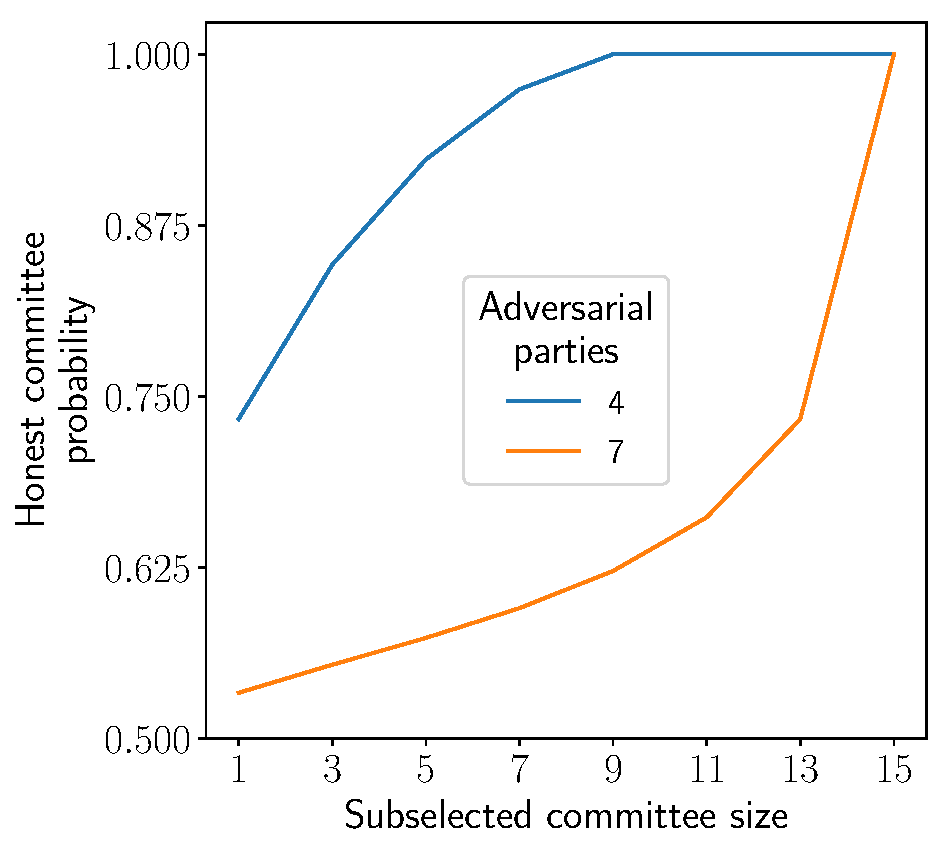
\includegraphics[width=0.5\columnwidth]{figures/collective-pools/probability_subselection.pdf}
    \end{center}
    \caption{
        The probability of subselecting an honest committee \wrt the committee
        size $\subselectionParam$, $\totalParties = 15$ total parties and
        $\lfloor \frac{\totalParties - 1}{3} \rfloor$ and $\lfloor
        \frac{\totalParties - 1}{2} \rfloor$ adversarial parties.
    }
    \label{fig:subselection}
\end{figure}

Following, Figure~\ref{fig:Fpool-2} defines the second part of our
functionality, while Figure~\ref{fig:Ppool-2} presents the second part of our
protocol.

\myhalfbox{Collective Pool Functionality $\Fpool^{\thold,\wfunc}$ (second part)}{white!40}{white!10}{
    \noindent{\bf Transaction Verification:}
        Upon receiving $\msg{transaction}{\tx, \subselectionParam}$ from
        $\p_i$, forward it to $\iadv$. Then send $\mathsf{READ}$ to $\Gledger$
        on behalf of $\p_i$ and wait for the reply $\chain$. Following, set
        $\adversarialParties$ as the number of corrupted parties; with
        probability $\prob^{\subselectionParam, \adversarialParties,
        \totalParties}$ set $b := \algovalidate(\tx, \chain)$, otherwise (with
        probability $1 - \prob^{\subselectionParam, \adversarialParties,
        \totalParties}$), send $\msg{transaction-ver}{\tx}$ to $\iadv$, wait for a reply
        $\msg{transaction-ok}{\chain, \tx, f}$, and set $b := f$. Finally, if
        $b = 1$, insert $\tx$ to $\mathsf{mempool}$ and send
        $\msg{transaction}{\chain, \tx, b}$ to all parties.

    \noindent{\bf Mempool Update:}
        Upon receiving $\msg{transaction}{\chain^\prime, \tx, 1}$ from $\p_i$,
        forward it to $\iadv$. Then send $\mathsf{READ}$ to $\Gledger$ on
        behalf of $\p_i$ and wait for the reply $\chain$. If $\chain^\prime \prec
        \chain$ and $\p_i$ is honest, insert $\tx$ to $\mathsf{mempool}$ and
        return $\msg{mempool-updated}{\tx}$.

    \noindent \noindent{\bf Block issuing:}
        Upon receiving $\msg{issue-block}{}$ from a party $\p$, forward it to
        $\iadv$. When a set of parties $\partyset$ has submitted
        $\msg{issue-block}{}$, if $\sum_{j \in [1, m]} \members[\p_j] >
        \thold$, then for every party $\p_i \in \partyset$, send
        $\mathsf{READ}$ to $\Gledger$ on behalf of $\p_i$ and wait for the
        reply $\chain_i$. If all received chains equal, \ie are the same chain
        $\chain$, remove every $\tx$ in $\mathsf{mempool}$ that also exists in
        $\chain$. Then, set $b = \blockify(\mathsf{mempool})$, send
        $\msg{issue-block}{b}$ to $\iadv$, and wait for the reply
        $\msg{issue-block}{b, \threshsig_{pool}}$.  Following, check if
        $\forall (m, \sigma, b^\prime) \in T: \sigma \neq \threshsig_{pool},
        (b, \threshsig_{pool}, 0) \not \in T$; if the checks hold, insert $(b,
        \threshsig_{pool}, 1)$ to $T$. Finally, reply with $\msg{block}{b,
        \threshsig_{pool}}$.

}{\label{fig:Fpool-2} The second part of the proposed Pool Functionality, which defines the consensus participation operations.}

\myhalfbox{Collective Pool Protocol $\Ppool^{\thold,\wfunc}$ (second part)}{white!40}{white!10}{
    \noindent{\bf Transaction Verification:}
        Upon receiving $\msg{transaction}{\tx, \subselectionParam}$, send
        $\mathsf{READ}$ to $\Gledger$ and wait for the reply $\chain$. Then,
        set $b = \algovalidate(\chain, \tx)$, compute $\partylist^\prime =
        \permutationAlgo(\tx, \chain, \partylist)$ and initiate protocol
        $\Pconsensus$ with the $\subselectionParam$ first parties in
        $\partylist^\prime$ with input $b$. Upon computing the output of
        $\Pconsensus$, $\beta$, send $\msg{transaction}{\chain, \tx, \beta}$ to
        $\Fbroad$ and return it.

    \noindent{\bf Mempool Update:}
        Upon receiving $\msg{transaction}{\chain^\prime, \tx, 1}$, $\p_i$, send
        $\mathsf{READ}$ to $\Gledger$ and wait for the reply $\chain$. If
        $\chain^\prime \prec \chain$, insert $\tx$ to $\mathsf{mempool}$ and return
        $\msg{mempool-updated}{\tx}$.

    \noindent{\bf Block Issuing:}
        Upon receiving $\msg{issue-block}{}$, send $\mathsf{READ}$ to
        $\Gledger$ and wait for the reply $\chain$. For every $\tx$ in
        $\mathsf{mempool}$, if $\tx$ is also in $\chain$, then remove $\tx$
        from $\mathsf{mempool}$. Next, set $b = \blockify(\mathsf{mempool})$
        and send $\msg{Sign}{b}$ to $\Fweight$. Upon receiving a reply
        $\msg{Sign}{b, \threshsig_{pool}}$, return $\msg{block}{b,
        \threshsig_{pool}}$.

}{\label{fig:Ppool-2} The second part of our protocol, which describes the set of operations for consensus participation.}

We note that our design satisfies most of the desiderata outlined in
Section~\ref{sec:collective-pool-desiderata}. Some (\eg pool proportional rewards or stake
reallocation) are dependent on the underlying ledger system's details,
therefore are outside of our scope; nevertheless, our design does not pose
restrictions in capturing them. The reward functionality $\rewardFunc$ handles
the reward-specific desiderata, while $\Fpool$'s first part
(Figure~\ref{fig:Fpool-1}) covers the requirements for permissioned access and
closing of the pool. However, $\Fpool$'s handling of stake reallocation and
updating of the pool's parameters could be more dynamic, as it currently
requires closing and re-creating a pool with the new parameters.

\section{Security Analysis}\label{sec:security}

We now assess the security of our collective pool design. Specifically,
Theorem~\ref{thm:collective-pool} shows that the protocol $\Ppool$ securely
realizes the ideal functionality $\Fpool$, assuming that the employed
cryptographic primitives are secure and that the adversarial power within the
pool is properly bounded.

\begin{theorem}\label{thm:collective-pool}
    The protocol $\Ppool$, parameterized by a validation predicate
    $\algovalidate$, a permutation algorithm $\permutationAlgo$, and a consensus
    protocol $\Pconsensus$ (cf. Definition~\ref{def:consensus})
    securely realizes $\Fpool$ with the hybrid execution $\hybpool$ in the
    global $\Gledger$ model, and
    $\prob^{\subselectionParam, \adversarialParties, \totalParties} = 1 - \sum_{v = \lfloor \frac{\subselectionParam + 1}{2} \rfloor}^{\min (\subselectionParam, \adversarialParties)} \frac{ {\adversarialParties \choose v} \cdot {{\totalParties - \adversarialParties} \choose {\subselectionParam - v}} }{ {\totalParties \choose \subselectionParam} }$,
    assuming $\sum_{\party \in P_{\adversary}} \weight_{\party} < \thold$, where
    $\subselectionParam$ is the subselection parameter for transaction
    verification, $P_{\adversary}$ is the set of $\adversarialParties$ corrupted
    parties out of $\totalParties$ total parties, $\wfunc$ is the weight
    distribution of the $\totalParties$ parties, and $\thold$ is the signature
    threshold.
\end{theorem}

\begin{proof}
    The proof is constructed in the UC Framework, so it is simulation-based. As
    such, we will show that the environment $\env$ cannot efficiently
    distinguish between two executions, the ideal and the real.  The simulator
    $\iadv$ interacts with the ideal functionality $\Fpool$ in the ideal
    execution, whereas $\adv$ interacts with $\Ppool$ in the real execution. We
    will show that, if $\Ppool$ does not securely realize the ideal
    functionality $\Fpool$, when instantiated with the parameters defined in
    the theorem, then at least one of the conditions is violated.

    First, we provide the construction for the simulator. $\iadv$ runs
    internally a copy of the adversary $\adv$. $\iadv$ forwards any inputs
    received from the environment $\env$ to the internal copy of $\adv$, and
    vice versa, and behaves as follows:
    \begin{itemize}
        \item \emph{Gathering}: Upon receiving the message $\msg{gather}{}$ for
            all parties $\party_i, i \in [1, \totalParties]$ from $\Fpool$, send
            $\msg{KeyGen}{}$ to $\Fweight$ with the appropriate $sid$.  Upon
            receiving the reply $\msg{KeyGen}{\threshpubkey_{pool}}$, record
            $\threshpubkey$, and return $\msg{gather-ok}{\threshpubkey}$ to
            $\Fpool$.
        \item \emph{Pool Registration}: Upon receiving the
            $\totalParties$ messages $\msg{register}{\mathsf{members}}$ from $\Fpool$, send
            $\msg{init}{\mathsf{members}}$ to $\rewardFunc$ and wait for
            $\msg{init-ok}{\addr_{reward}}$.  Then send $\msg{Sign}{m}$
            to $\Fweight$ with $m = (\mathsf{members}, \addr_{reward}$). Upon
            receiving a reply $\msg{Sign}{m, \threshsig_{pool}}$, register $(m,
            \threshsig_{pool})$ and return to $\Fpool$ the message
            $\msg{register-ok}{\addr_{reward}, \threshsig_{pool}}$.
        \item \emph{Closing}: Upon receiving $\msg{close}{x}$ from $\Fpool$, on
            behalf of a set of parties $\partyset$, send the message
            $\msg{Sign}{x}$ to $\Fweight$ on behalf of each party in
            $\partyset$.  Upon receiving a reply $\msg{Sign}{x,
            \threshsig_{pool}}$, record $\threshsig_{pool}$ and return
            $\msg{close-ok}{\threshsig_{pool}}$ to $\Fpool$.
        \item \emph{Transaction Verification}: Upon receiving
            $\msg{transaction-ver}{\tx}$ from $\Fpool$, forward it to the
            internal copy of $\adv$, wait for the output
            $\msg{transaction-ok}{\chain, \tx, f}$ from $\adv$ and forward it
            to $\Fpool$.
        \item \emph{Block issuing}: Upon receiving $\msg{issue-block}{b}$ from
            $\Fpool$, send $\msg{Sign}{b}$ to $\Fweight$. Upon receiving a
            reply $\msg{Sign}{b, \threshsig_{pool}}$ and record $(b,
            \threshsig_{pool})$.  Finally, return $\msg{issue-block}{b,
            \threshsig_{pool}}$ to $\Fpool$.
        \item \emph{Party corruption}: When the adversary $\adv$ corrupts a
            party $\party$, $\iadv$ corrupts the same party in the ideal process
            and hands to $\adv$ its internal state.
        \item \emph{Global ledger update}: When $\adversary$ sends
            $(\mathsf{ADVANCE}, \party, \Sigma)$ to the global ledger $\Gledger$,
            $\iadv$ does so in the ideal world; similarly, when
            $\adversary$ sends $(\mathsf{EXTEND}, b)$ to $\Gledger$, so does
            $\iadv$.
        \item \emph{Signature generation}: When the adversary $\adv$ requests a
            signature on some message $m$, $\iadv$ sends $\msg{Sign}{m}$ to
            $\Fweight$; upon receiving the reply $\msg{Sign}{m, \threshsig}$,
            it returns $\threshsig$ to $\adv$.
    \end{itemize}

    The first observation is that $\iadv$ needs to ensure that a party $\party$ has
    the same view of the ledger as in the real world. Therefore, it advances
    parties only when the real world adversary $\adv$ does so.

    To prove the theorem, we assume that $\Ppool$ does not realize $\Fpool$,
    \ie there exists adversary $\adversary$ such that, for every simulator
    $\iadv$, there exists environment $\env$ that can distinguish between the
    ideal world (of $\Fpool$ and $\iadv$) and the real world (of $\Ppool$ and
    $\adversary$). Following, we show that $\iadv$ violates the security of one
    of the primitives used by $\Ppool$, \ie the consensus protocol
    $\Pconsensus$ and the weighted threshold signature scheme
    $\threshsigscheme$.

    We build an algorithm $\distinguisher$ that breaks the security of the
    cryptographic primitives as follows.  $\distinguisher$ runs a simulated
    copy of $\env$ and simulates for $\env$ the ideal environment, \ie
    $\distinguisher$ acts both as $\Fpool$ and $\iadv$ on $\env$'s messages.

    Similar to $\iadv$, $\distinguisher$ runs a simulated copy of $\adv$. When
    running \emph{Gathering} to obtain the threshold keys, instead of running
    $\threshkeygen$, $\distinguisher$ hands $\adversary$ the public key
    $\threshpubkey$ which is obtained as the input from $\iadv$. To obtain a
    signature $\signature$ on a message $m$, $\distinguisher$ hands $m$ to its
    oracle, instead of using $\threshsign$. When $\adv$ advances the state of
    party $\party$ in the global ledger $\Gledger$, $\distinguisher$ does so as
    well.

    Regarding the consensus subprotocol $\Pconsensus$, we consider the case
    when $\env$ activates an uncorrupted party $\party$ with input a transaction
    $\tx$ via the interface \emph{Transaction Verification}. At that point,
    $\distinguisher$ computes $b = \algovalidate(\chain, \tx)$, where $\chain$
    is the state of party $\party$ in the global ledger $\Gledger$. Next,
    $\distinguisher$ checks the output $b'$ in the real world (where
    $\adversary$ operates). If the majority of the committee elected to
    validate $\tx$ is honest and $b \neq b'$, then $\distinguisher$ retrieves
    the transcript of $\Pconsensus$, run for the validation of $\tx$ by
    $\adversary$, and outputs it (observe that this transcript is represents an
    execution of $\Pconsensus$ where its security breaks).

    To analyze the success probability of $\distinguisher$, we consider the
    event $E$, where $b \neq b'$, as defined above. Since $\Pconsensus$ is
    secure as long as a majority of participants is honest, the executions of
    the real world, \ie the interaction of $\env$ with $\adversary$ and
    $\Ppool$, and the ideal world (resp. $\iadv$ and $\Fpool$) are
    statistically close. If we are guaranteed that $\env$ distinguishes between
    the two executions, then $E$ occurs with non-negligible probability.
    Finally, from the point of view of $\adversary$ and $\env$, the interaction
    with $\distinguisher$ is the same as with an interaction with protocol
    $\Ppool$ in the real world.

    Regarding the weighted threshold signatures, we note that the functionality
    $\Fpool$ performs the same checks regarding signature issuing as
    $\Fweight$. In fact, only signature generation is performed by the
    collective pool; signature verification should be employed when advancing
    the ledger state, \ie upon adopting new blocks, or when validating a
    certificate. Therefore, the security of $\Fweight$ ensures that $\env$
    cannot distinguish the two executions (real vs. ideal world) \wrt the
    weighted threshold signatures.

    Regarding block issuing we consider the event $E'$, where a set of parties
    controlling a majority of the pool's stake initiate block issuing, but no
    signed block is output. In that case, either the signature issuing of
    $\threshsigscheme$ fails or the parties locally produce a different block
    $b$, \ie their mempool is not synchronized. Regarding the former, the
    same analysis on signature issuing as above applies. Regarding the latter,
    if two honest parties hold a different mempool at the point when
    $\blockify$ is used, either their ledger state $\chain$ is different or
    their mempool is different. This implies that $\Fbroad$ fails for at least
    one transaction $\tx$, \ie an honest party inserts $\tx$ in its mempool
    and, after $\tx$ is sent to $\Fbroad$, at least one other honest party
    fails to also insert it to its mempool. However, this is impossible, since
    the simulator ensures the former and $\Fbroad$ ensures the latter.

    Finally, the permutation algorithm $\permutationAlgo$ is executed locally
    by each party, therefore the adversary cannot affect its output.
    Additionally, the probability $\prob^{\subselectionParam,
    \adversarialParties, \totalParties}$ is computed following the analysis of
    Section~\ref{sec:participation}.
\end{proof}

\section{Incentives Analysis}\label{sec:incentives}

Although, as shown in Theorem~\ref{thm:collective-pool}, $\Ppool$ is secure, it
is unclear whether rational users will opt for using it. In this section, we
discuss the incentive compatibility of $\Ppool$. We identify its shortcomings
and propose a minor change, such that rational members cannot gain more rewards
by deviating from it.

First, we consider the cost of each operation performed in $\Ppool$. Signing
operations does not incur any cost, thus pool registration and revocation are
cost-free. Block production depends on the internal workings of $\blockify$.
For instance, solving the Knapsack problem can be expensive, while a greedy
algorithm that prioritizes high-fee transactions is typically not. Therefore,
without loss of generality, we also assume that block production is cost-free.
However, both mempool update and transaction verification incur costs
$\cost_{mu}$ and $\cost_{tv}$ respectively. A mempool consists of millions of
transactions and verifying them requires an accurate view of the
ledger. Thus, both objects may require significant amounts of computations
and storage.\footnote{As of January 2021, the Bitcoin chain is
roughly $320$GB and increases linearly over time.
(\url{https://www.blockchain.com/charts/blocks-size})}

We focus on the \emph{profit} of each member, \ie the rewards subtracted by
the cost of executing $\Ppool$. The core observation is that a member $\party$
receives $\reward_{\party} = \frac{\weight_{\party}}{\sum_{\party' \in \wfunc}
\weight_{\party'}}$ of the total pool's rewards \emph{regardless of its
performance}. For instance, if $\party$ acts only on the pool's
creation, it still receives its proportional share of rewards for the blocks
produced by the rest of the pool. Therefore, as long as a member believes that
the other members act honestly, it is incentivized to abstain and minimize its
cost, thus maximizing its profit. Naturally, if all parties follow this
strategy, the pool produces no blocks and receives no rewards.

A possible solution to the Free Rider problem above is to penalize a party
for misbehaving.  However, identifying misbehavior is not straightforward. For
instance, a party $\party$ who inputs $0$ to $\Pconsensus$ for a transaction
$\tx$ may do so either because the transaction is invalid or because it
didn't perform validation and input $0$ by default. Our approach is to
penalize a party when diverging from the rest of the pool. In the previous
example, if the output of $\Pconsensus$ is $1$, then $\party$ incurs a fixed
penalty $P_{tv}$. Similarly, if a party fails to sign a new block
then it incurs a (fixed) penalty $P_{mu}$. The penalty amount,
which is withheld from $\party$, is then distributed equally among the other
pool members.  To incentivize $\party$ to follow $\Ppool$ the penalties should
be high enough; specifically, it should hold $P_{tv} >
\cost_{tv}$ and $P_{mu} > \cost_{mu}$.  If all parties follow
$\Ppool$, diverting incurs a cost $P_{mu} - \cost_{mu} > 0$
(resp. $P_{tv} - \cost_{tv} > 0$), thus the new protocol is an
equilibrium.

Finally, penalties can be automatically enforced via an interface to the smart
contract $\rewardFunc$ which, given a proof of misbehavior, reduces the
misbehaving party's rewards accordingly. For transaction verification, a proof
of misbehavior is the transcript of $\Pconsensus$, which describes the
consensus sub-protocol's execution. For block issuing, we can use a threshold
signature scheme with identifiable aborts~\cite{EPRINT:GenGol20,CCS:CGGMP20},
which allows to identify the parties that do not participate in the signing of
a block.


\chapter{
    Efficient Global State Management
}\label{chap:utxo-growth}

Distributed ledgers implement a storage layer, on top of which a shared state
is maintained in a decentralized manner. In ledger systems, this state
consists of three objects:
\begin{inparaenum}[i)]
    \item the public ledger, \ie the list of transactions which form the
        system's history;
    \item the mempool, \ie the set of, yet unpublished, transactions;
    \item the active state which, in systems like Bitcoin, consists of the UTxO
        set.
\end{inparaenum}
To support thousands (or millions) of participants, a decentralized system's
state management should be well-designed, primarily focused on minimizing the
shared state. Our work focuses on the third type, as poorly designed management
often leads to performance issues and even Denial-of-Service (DoS) attacks. In
Ethereum, during a 2016 DoS attack, an attacker added 18 million accounts to
the state, increasing its size by 18 times~\cite{ethereum-dos}. Bitcoin saw
similar spam attacks in 2013~\cite{FCW:VasThoMoo14} and
2015~\cite{bitcoin-flooding}, when millions of outputs were added to the UTxO
set.

Mining nodes and full nodes incur costs for maintaining the shared state in the
Bitcoin network. This cost pertains to the resources (\ie CPU, disk, network
bandwidth, memory) that are consumed with every transaction transmitted,
validated, and stored. An expensive part of a transaction is the newly created
outputs, which are added to the in-memory UTxO set. As the system's scale
increases, the cost of maintaining the UTxO set gradually leads to a
shared-state bloat, which makes the cost of running a full node prohibiting.

Moreover, the system's incentives, which are promoted via transaction fees,
only deteriorate the problem. For example, assume two transactions $\tx_A$ and
$\tx_B$: $\tx_A$ spends $5$ inputs and creates $1$ output, while $\tx_B$ spends
$1$ input and creates $2$ outputs. Assuming the size of a UTxO is equal to the
size of consuming it (200 bytes) and that transaction fees are $30$ satoshi per
byte, $\tx_A$ costs $30 \times 200 \times (5+1) =  36000$ satoshi and $\tx_B$
costs $30 \times 200 \times (1+2) = 18000$ satoshi. Although $\tx_B$ burdens
the UTxO set by creating a net delta of ($2 - 1 = 1$) new UTxO, while $\tx_A$
reduces the shared state by consuming ($1 - 5 = -4$) UTxOs, $\tx_B$ is cheaper
in terms of fees. Clearly, the existing fee scheme penalizes the consumption of
multiple inputs, disincentivizing minimizing the shared state.

\paragraph{Related Work}
The problem of unsustainable growth of the UTxO set has concerned developers
for years. It has been discussed in community
articles~\cite{bitcoin-mag-utxo,state-growth-problem},
some~\cite{andresen-utxo} offering estimations on the level of inefficiency in
Bitcoin. Additionally, research
papers~\cite{EPRINT:PDNH18,EPRINT:DPNH17b,houyBitcoin,easley2019mining} have
analyzed Bitcoin's and other cryptocurrencies' UTxO sets to gain further
insight. Engineering efforts, \eg in Bitcoin Core's newer
releases~\cite{maxwell-core}, have also focused on improving performance by
reducing the UTxO memory requirements. Various solutions have been proposed to
reduce the state of a UTxO ledger, \eg consolidation of
outputs~\cite{bitcoin-utxo-consolidate} can help reduce the cost of spending
multiple small outputs. Alternatively, Utreexo~\cite{EPRINT:Dryja19}, uses
cryptographic accumulators to reduce the size of the UTxO set in memory, while
BZIP~\cite{jiang2019bzip} explores lossless compression of the UTxO set.

An important notion in this line of research is the ``stateless
blockchain''~\cite{todd-utxo}. Such blockchain enables a node to participate in
transaction validation without storing the entire state of the blockchain, but
only a short commitment to it. Chepurnoy \etal~\cite{EPRINT:ChePapZha18} employ
accumulators and vector commitments to build such blockchain. Concurrently,
Boneh \etal~\cite{EPRINT:BonBunFis18b} introduce batching techniques for
accumulators in order to build a stateless blockchain with a trustless setup
which requires constant amount of storage. We consider an orthogonal problem,
\ie constructing transactions in an incentive-compatible manner that minimizes
the state, so these tools can act as building blocks in our proposed
techniques.

The role of fees in blockchain systems has also been a topic of interest in
recent years. Luu \etal~\cite{CCS:LTKS15} explored incentives in Ethereum,
focusing on incentivizing miners to correctly verify the validity of scripts
run on this ``global consensus computer''. M{\"o}ser and
B{\"o}hme~\cite{FCW:MosBoh15} investigate Bitcoin fees empirically and observe
that users' behavior depends primarily on the client software, rather than a
rational cost estimation. Finally, in an interesting work, Chepurnoy
\etal~\cite{FCW:CheKhaMes18} propose a fee structure that considers the
storage, computation, and network requirements; their core idea is to classify
each transaction on one of the three resource types and set its fees
accordingly.

\paragraph{Contributions}
Our work investigates techniques that minimize the shared state of the
distributed ledger, \ie the in-memory UTxO set. Our approach is twofold:
\begin{inparaenum}[a)]
    \item we propose transaction optimization techniques which, when employed
        by wallets, help reduce the shared state's cost;
    \item propose a novel fee scheme that incentivizes ``shared
        state-friendly'' transactions.
\end{inparaenum}

In particular, we propose a UTxO model, which abstracts UTxO ledgers and
enables evaluating the cost of a ledger’s shared state. We then
propose a transaction optimization framework, based on three levels of
optimization:
\begin{inparaenum}[a)]
    \item a declarative (rule-based) level,
    \item a logical/algebraic (cost-based) level, and
    \item a physical/algorithmic (cost-based) level.
\end{inparaenum}
Following, we propose three transaction optimization techniques based on the
aforementioned optimization levels:
\begin{inparaenum}[a)]
    \item a rule-driven optimal total order of transactions (the
        \emph{last-payer rule}),
    \item a logical transaction transformation (the \emph{2-for-1
        transformation}), and
    \item a novel \emph{input selection} algorithm that minimizes the UTxO set
        increase, \ie favors consumption over creation of UTxOs.
\end{inparaenum}
We then define the transaction optimization problem and propose a 3-step
dynamic programming algorithm to approximate the optimal solution.  Finally, we
define the state efficiency property that a fee function should have, in order
to correctly reflect a transaction's shared-state cost, and propose a state
efficient fee function for Bitcoin.

\section{A UTxO Model}\label{sec:utxo_model}

We abstract a distributed ledger as a state machine on which parties act.
Specifically, we consider only \emph{payments}, \ie value transfers of
\emph{fungible} assets between parties.

Initially, we assume a ledger state $\ledgerState_{init}$, on which a
\emph{transaction} is applied to move the ledger to a new state. Transactions
that may be applied on a state are \emph{valid}, following a validation
predicate. Each transaction is unique and moves the system to a unique state;
with hindsight, we assume that the ledger never transitions to the same state
(cf. Definition~\ref{def:lstate}), \ie valid transactions do not form cycles.
Figure~\ref{fig:state-machine} provides intuition via a simple ledger model.

\begin{figure}
    \centering

    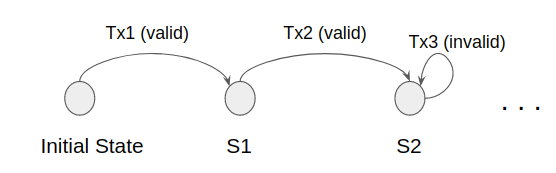
\includegraphics[width=0.6\textwidth,keepaspectratio]{figures/utxo_growth/state_machine.png}
    \caption{A decentralized state machine model for a distributed ledger.}
    \label{fig:state-machine}
\end{figure}

Our formalism is similar to chimeric ledgers~\cite{chimeric}, though focused on
UTxO-based ledgers. Following, we provide some basic definitions in a
``top-down'' approach, starting with the ledger $\ledger$, which is an ordered
list of transactions; our notation of functions is the one typically
used in functional programming languages, for example a function $f : A
\rightarrow B
\rightarrow C$ takes two input parameters of type $A$ and $B$ respectively and
returns a value of type $C$.

\begin{definition}
    A \emph{ledger} $\ledger$ is a list of valid transactions: $\ledger \defn \mathit{List}[\mathit{Transaction}]$.
\end{definition}

A transaction $\tx$ transitions the system from one state to another.
UTxO-based transactions are thus a product of \emph{inputs}, which define the
ownership of assets, and \emph{outputs}, which define the rules of
re-transferring the acquired value.

\begin{definition}
    A UTxO-based transaction $\tx$ is :
    $\mathit{Transaction} \defn (\mathit{inputs}: \mathit{Set}[\mathit{Input}],
                       \mathit{outputs}: \mathit{List}[\mathit{UTxO}],
                       \mathit{forge}: \mathit{Value},
                       \mathit{fee}: \mathit{Value})$
\end{definition}

An \emph{unspent transaction output (UTxO)} represents the ownership of some
value from a party, which is represented via an \emph{address} $\addr$.
Intuitively, in the real world, an output is akin to owning a physical coin of
an arbitrary denomination.

\begin{definition}\label{def:utxo}
    A UTxO is defined as follows: $\mathit{UTxO} \defn (\addr: \mathit{Address},\ \mathit{value}: \mathit{Value},\ \mathit{created}: \mathit{Timestamp})$.
\end{definition}

A transaction's input is a reference to a UTxO, \ie an output that is owned by
the party that creates the transaction. An input consists of two objects:
\begin{inparaenum}[i)]
    \item the \emph{id} of the transaction that created it (typically its hash)
        and
    \item an index, which identifies the specific output among all UTxOs of the
        referenced transaction.
\end{inparaenum}

\begin{definition}
    An input is defined as: $\mathit{Input} \defn (\mathit{id}: \mathit{Hash}, \mathit{index}: \mathit{Int})$.
\end{definition}

Given an input and a ledger, three functions retrieve:
\begin{inparaenum}[i)]
    \item the corresponding output,
    \item the corresponding transaction, and
    \item the input value.
\end{inparaenum}
All returned values are wrapped in \verb|Option|, denoting that a value may not
be returned.

\begin{itemize}
    \item $\utxo: \inp \rightarrow \ledger \rightarrow \verb|Option|[\utxo]$
    \item $\tx: \inp \rightarrow \ledger \rightarrow
        \verb|Option|[\mathit{Transaction}]$
    \item $\mathit{value}: \inp \rightarrow \ledger \rightarrow \verb|Option|[\mathit{Value}]$
\end{itemize}

A transaction defines some value that is given as a \emph{fee} to the
\emph{miner}, \ie the party who publishes the transaction into the ledger
$\ledger$. We require that all transactions must preserve value as
follows:
$\tx.\mathit{forged} + \sum_{i \in \tx.\mathit{inputs}}^{} \mathit{value}(i, \ledger) = \tx.\mathit{fee} + \sum_{o \in \tx.\mathit{outputs}}^{} o.\mathit{value}$.
We note that this applies only on standard transactions, not ``coinbase''
transactions which create new coins.

Finally, we define the ledger's state $\ledgerState$. $\ledgerState$ comprises
the \emph{UTxO set}, \ie the set of all outputs of transactions whose value
has not been re-transferred and can be used as inputs to new transactions.

\begin{definition}\label{def:lstate}
    The ledger's state is defined as: $\mathit{State} \defn \mathit{Set}[\mathit{Input}]$.
\end{definition}

We now return to the state machine model. A transaction is applied on a ledger
state $\ledgerState_1$ and results in a ledger state $\ledgerState_2$ via the
function:
\begin{align*}
    \mathsf{txRun}: \mathit{Transaction} \rightarrow \mathit{LedgerState} \rightarrow \mathit{LedgerState}
\end{align*}
An ordered list of transactions $\txSet = [\tx_1, \tx_2, \dots, \tx_N]$ can be
applied sequentially on state $\ledgerState_1$ to transit to state
$\ledgerState_N$: $\ledgerState_N = (\mathsf{txRun}(\tx_N).\; \dots\;
.\mathsf{txRun}(\tx_2) .  \mathsf{txRun}(\tx_1))(\ledgerState_1)$, assuming the
function composition operator (.).

Finally, every ledger state $\ledgerState$ corresponds to some cost
$\stateCost$.  We assume a cost function, which assigns a signed integer of
cost units to a ledger state.
\begin{align*}
    \mathsf{cost}: \mathit{LedgerState} \rightarrow \mathit{Cost}
\end{align*}
This function is employed in
Definition~\ref{def:tx-cost}, which defines a transaction's cost; minimizing
this cost will be the target of our optimization. Observe that the
transaction's cost might be negative, \eg if the transaction reduces the state.

\begin{definition}\label{def:tx-cost}
    The cost of a transaction $\tx$ applied to a state $\ledgerState$ is the
    difference between the cost of the final state minus the cost of the
    initial state:

    \begin{math}\\
        \mathsf{costTx}: \mathit{Transaction} \rightarrow \mathit{LedgerState} \rightarrow \mathit{Cost} \\
        \mathsf{costTx}(\tx, \ledgerState) = cost(\mathsf{txRun}(\tx,
        \ledgerState)) - \mathit{cost}(\ledgerState)\\
    \end{math}

        The cost of an ordered list of transactions $[T]$ applied to a state
        $\ledgerState$ is the difference between the cost of the final state
        minus the cost of the initial state:

	\begin{math}\\
            \mathsf{costTotTx}: [\mathit{Transaction}] \rightarrow \mathit{LedgerState} \rightarrow
                \mathit{Cost}\\
		\mathsf{costTotTx}([T], \ledgerState) =
                        \mathit{cost}((\mathsf{txRun}(\tx_N).\; \dots\; .\mathsf{txRun}(\tx_2) .
                        \mathsf{txRun}(\tx_1))(\ledgerState_1)) - \mathit{cost}(\ledgerState)
	\end{math}
\end{definition}

We note that cost represents the size of the ledger's state. However, our model
is generic enough to accommodate alternative cost designs as well. For
instance, cost could represent the computational effort of producing or
verifying the state, such that a cost unit would be a computational cycle.
Therefore, our analysis would also be directly applicable in that case, by
accordingly adapting some parts of the subsequent optimization framework like
the heuristics.

\section{Transaction Optimization}\label{sec:tx_optimization}

The purpose of a distributed ledger is to execute payments, \ie transfer value
from one party to another via transactions.  Multiple transactions can perform
the same transfer of value between two parties. Such transactions are
\emph{equivalent} in terms of their final result, \ie transferring some value
between parties A and B, but may vary in their cost to the ledger state.
\emph{Transaction optimization} is the problem of finding the equivalent
transaction with minimum cost; our work is heavily inspired by the seminal
research on database query optimization \cite{ioannidis}.

The cost difference between equivalent transactions may be significant.
For example, assume that Alice wants to give Bob $100$ coins and owns a UTxO of
$100$ coins and $100$ UTxOs of $1$ coin each. Consider the two equivalent
plans:
\begin{inparaenum}[1)]
    \item Alice spends the single UTxO of value $100$ and
        creates $100$ outputs of value $1$ for Bob;
    \item Alice spends the $100$ UTxOs of $1$ coin value and
        defines a single UTxO of value $100$ to transfer to Bob.
\end{inparaenum}
The cost of the two approaches exemplifies the ledger state impact that
equivalent transactions may have. The first plan increases the ledger's state
by $99$ UTxOs, while the second decreases it by the same amount.

Following, we use the terms plan and transaction interchangeably, \ie an
alternative plan that achieves the same goal is expressed as an alternative,
equivalent transaction. Definition~\ref{def:equiv_txs} describes transaction
equivalency, while Definition~\ref{def:equiv_total_orders_of_txs} defines
equivalency between two ordered lists of transactions.

\begin{definition}\label{def:equiv_txs}
    Transactions $\tx_1, \tx_2$ are equivalent (denoted $\tx_1
    \equiv \tx_2$) if, when applied to the same state $\ledgerState_A$
    of a ledger $\ledger$, they result in states $\ledgerState_1$ and
    $\ledgerState_2$ respectively, with the same total accumulated value per unique
    address $\addr$:
    \[
    \forall \addr \in A
        \sum_{\substack{i \in \ledgerState_1 \\ o_i = \utxo(i, \ledger) \\
        o_i.\mathit{address} =
        \addr }}^{} o_i.\mathit{value} =
        \sum_{\substack{ j \in \ledgerState_2 \\ o_j = \utxo(j, \ledger) \\
        o_j.\mathit{address} =
        \addr }}^{} o_j.\mathit{value}
    \]
    where $A$ is the set of all addresses of the parties participating in the
    ledger system.
\end{definition}

\begin{definition}\label{def:equiv_total_orders_of_txs}
    Two different totally ordered sets of the same $N$ transactions $[T_i]$ and
    $[T_j]$ are equivalent (denoted as $[T_i]
    \equiv [T_j]$) if, when applied to the same ledger state $\ledgerState_A$
    of a ledger $\ledger$, they result in states $\ledgerState_1$ and
    $\ledgerState_2$ respectively, where the total accumulated value per unique
    address $\addr$ is the same in both states:
    \[
    \forall \addr \in A
    \sum_{\substack{i \in \ledgerState_1 \\ o_i = \utxo(i, \ledger) \\
        o_i.\mathit{address} =
        \addr }}^{} o_i.\mathit{value} =
    \sum_{\substack{ j \in \ledgerState_2 \\ o_j = \utxo(j, \ledger) \\
        o_j.\mathit{address} =
        \addr }}^{} o_j.\mathit{value}
    \]
    where $A$ is the set of addresses of all participants in the distributed
    ledger system.
\end{definition}

Following, we define the basic logical operators for expressing a transaction
and explore optimization techniques for compiling the optimal transaction plan.

\subsection{Transaction Logical Operators - Ledger State Algebra}\label{sec:logical-operators}

First, we introduce some basic \emph{logical} operators, \ie functions used to
form a transaction. The operators are regarded as basic logical steps for
executing a transaction, \ie irrespective of their particular implementation.
However, depending on their implementation, each step may correspond to
different cost. The operators operate on and produce a state, forming ---
possibly equivalent (cf. Definition~\ref{def:equiv_txs}) ---
\emph{transactions}. The operators and operands form a \emph{ledger state
algebra} and, as the state is a set of UTxOs (cf.
Definition~\ref{def:lstate}), all common set operators are applicable. In case
of failure, they return the empty state $\varnothing$. The three operators are
as follows:
\begin{itemize}
    \item \emph{Input Selection:}
        $\sigma_{(P_{id},V)} : LedgerState \rightarrow	LedgerState$

        $\sigma_{(P_{id},V)}$ is a unary operator, which is given as input
        parameter a pair \emph{(Party id, Value)}. \emph{Party id} is an
        abstraction of a set of UTxOs, \eg
        it could abstract a \emph{wallet} that controls a set of addresses,
        each owning multiple UTxOs.
        When applied on a state $\ledgerState_i$, $\sigma_{(P_{id},V)}$
        produces a new state $\ledgerState_f \subset \ledgerState_i$, where
        $\forall o \in \ledgerState_f: o \in P_{id}$ and $\sum_{o \in
        P_{id}}^{}o.value \geq V$. Essentially, $\sigma$ is a filter over a
        state, selecting the UTxOs with aggregate value larger than, or equal
        to the input
        $V$.

    \item \emph{Output Creation}
        $\pi_{[(a_1,v_1), \dots,(a_n,v_n)]} : LedgerState \rightarrow LedgerState$

        $\pi_{[(a_1,v_1), \dots,(a_n,v_n)]}$ is a unary operator, which is
        given a set of \emph{(Address, Value)} pairs and is applied on a state
        $\ledgerState_i$. It produces a new UTxO set $\ledgerState_f$ with
        $\ledgerState_f \cap \ledgerState_i = \varnothing$, \ie
        $\ledgerState_f$ includes only new UTxOs. Also $\forall o \in
        \ledgerState_f: (o.address, \sum_{o.address}^{}o.value) \in [(a_1,v_1),
        \dots a_n,v_n)]$, \ie the aggregate output value per address is equal
        to the input parameter. We require that value is preserved, \ie the
        total value in $\ledgerState_i$ is greater than (or equal to) the total
        value in $\ledgerState_f$; the value difference is is the miners' fee.

    \item \emph{Transaction Validation}
        $\tau_{V_R, \ledgerState_i} : LedgerState \rightarrow LedgerState \rightarrow LedgerState$

        $\tau_{V_R,\ledgerState_i}$ is a binary operator that validates input
        and output states $\ledgerState_I, \ledgerState_O$, against a set of
        rules $V_R$, over an initial state $\ledgerState_G$. If validation
        succeeds, it returns an updated state $\ledgerState_f = (\ledgerState_G
        - \ledgerState_I) \cup \ledgerState_O$.
\end{itemize}

Figure~\ref{fig:simplest_tx} depicts the simplest transaction under our
algebra, \ie a tree with a root and two branches. The root is the transaction
validation operator $\tx$, that receives two inputs:
\begin{inparaenum}[a)]
    \item the set of selected inputs ($\sigma$ on the left branch) and
    \item the set of outputs to be created ($\pi$ on the right branch).
\end{inparaenum}
We express this transaction algebraically as: $T = (\sigma_{Alice, V}) \infixOperator
(\pi_{Bob,V})$, $\infixOperator$ being the infix validation operator.

\begin{figure}[h!]
    \centering
    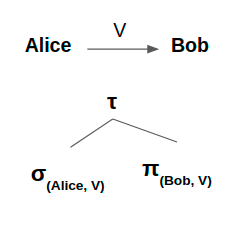
\includegraphics[width=0.3\columnwidth,keepaspectratio]{figures/utxo_growth/simplest_tx.png}
    \caption{The simplest expression of a transaction.}
    \label{fig:simplest_tx}
\end{figure}

Moving one step further, we assume three transactions $\tx_1$, $\tx_2$ and
$\tx_3$. The execution of these transactions is \emph{totally ordered}, \ie
$\tx_1 \rightarrow \tx_2 \rightarrow \tx_3$. Figure~\ref{fig:tx_order} depicts
this expression. Here, $\tx_1$ is nested within $\tx_2$ and both are nested
within $\tx_3$. Such tree is executed from bottom to top, therefore $\tx_2$ is
given the ledger state generated after $\tx_1$ is executed; similarly, $\tx_3$
is given the ledger state generated after both $\tx_1$ and $\tx_2$ are
executed. Given the above, we next define \emph{subtransactions};
interestingly, transactions may spend outputs created from their
subtransactions, thus we also define the notion of \emph{correlated
transactions}.

\begin{figure}[h!]
    \centering
    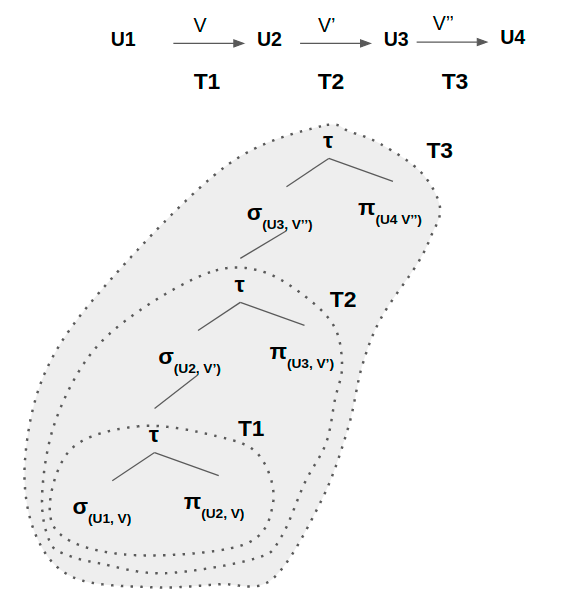
\includegraphics[width=0.5\columnwidth,keepaspectratio]{figures/utxo_growth/tx_order.png}
    \caption{The expression tree entails a transaction execution total
            order.}
    \label{fig:tx_order}
\end{figure}

\begin{definition} \label{def:subtransaction}
    A \emph{subtransaction} is a transaction nested within a ``parent''
    transaction; it is executed first, so its impact on the ledger state is
    visible to the parent.
\end{definition}

\begin{definition} \label{def:correlated_tx}
    Two transactions $\tx_1, \tx_2$ are correlated, if $\tx_1$ is a
    subtransaction of $\tx_2$ and $\tx_2$ spends at least one output created by
    $\tx_1$.
\end{definition}

\subsection{A Transaction Optimization Framework}\label{sec:tx_optimization_framework}

We now identify different phases in the transaction optimization process; in
a hypothetical \emph{transaction optimizer} each phase would be a distinct
module. These phases are different approaches to producing equivalent
transactions. The phases operate on three levels of optimization:
\begin{inparaenum}[a)]
    \item a declarative (rule-based) level,
    \item a logical/algebraic (cost-based) level, and
    \item a physical/algorithmic (cost-based) level,
\end{inparaenum}
as depicted in Figure~\ref{fig:optimization-phases}. The input of the process
is a transaction set $[\tx_x]$, that we want to optimize, and while output is the
optimal transaction $\tx_{x-Optimal}$.

\paragraph{Rules}
This phase is declarative, as it does not depend on the cost; instead, when
applied, it necessarily produces a better transaction. Essentially it consists
of \emph{heuristic rules} that are applied by default to produce an equivalent
transaction; example of such rules are ``create a single output per address''
or ``consume as many inputs and create as few outputs as possible''.

\paragraph{Algebraic Transformations}
These are transformations at the level of logical operators that define a
transaction's execution. Generally the efficiency of such transformation is
evaluated based on the entailed cost. Examples of such transformations are the
2-for-1 transformation (cf. Definition~\ref{def:2-for-1}) and different
transaction orderings (cf. Definition~\ref{def:subtransaction}).

\paragraph{Methods and Structures}
This phase optimizes the algorithm that implements a logical operator. For
instance, given two algorithms $A, B$ result in transaction costs $\cost_A, \cost_B$,
if $\cost_A < \cost_B$ we would choose $A$; one such example is the different
implementations of the input selection operator $\sigma$, as shown in
Figure~\ref{fig:3-logical-plans}. Optimizations in this phase may also change
the data structure used to access the underlying data, which in our case is the
ledger state.

\paragraph{Planning and Searching}
This phase employs a \emph{searching strategy} to explore the available space
of candidate solutions, \ie equivalent transaction plans. This space consists
of the transactions produced from the above phases, each evaluated based on
their cost, under the available cost model.

\begin{figure}[h!]
	\centering
	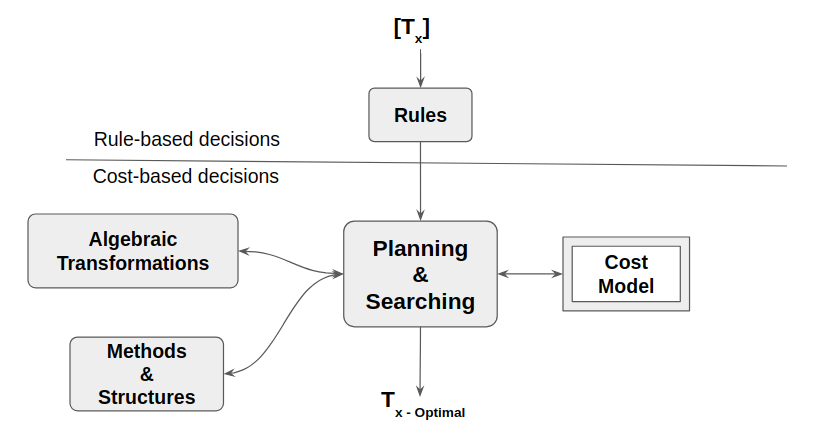
\includegraphics[width=0.8\columnwidth,keepaspectratio]{figures/utxo_growth/optimization_phases.png}
	\caption{The transaction optimization process.}
	\label{fig:optimization-phases}
\end{figure}

\subsection{Transaction Optimization Techniques}\label{sec:tx_optimization_techniques}

In this section, we propose three transaction optimization techniques
based on the aforementioned optimization levels:
\begin{inparaenum}[a)]
    \item heuristic rule-based,
    \item logical/algebraic transformation cost-based, and
    \item physical/algorithmic cost-based.
\end{inparaenum}

\subsubsection{Input Selection Optimization}\label{sec:input_sel_optimization}

We demonstrate this technique with an example. Assume Alice wants to give Bob
$5$ coins. Figure~\ref{fig:3-logical-plans} depicts three equivalent
transactions for implementing this payment. Observe that each plan is
represented as a tree, where the intermediate nodes are the previously defined
logical operators (that act on a ledger state) and the leaf nodes are ledger
states. We also assume that the state cost is the number of elements (UTxOs) in
the state.  The three transactions have the same structure, \ie they are the
same logical expression, but result to different ledger states with different
costs. The transactions differ only in the output of the input selection
operator ($\sigma_{(Alice, 5)}$), a difference which may be attributed to
different implementations of the operator.

\begin{figure}[h!]
    \centering
    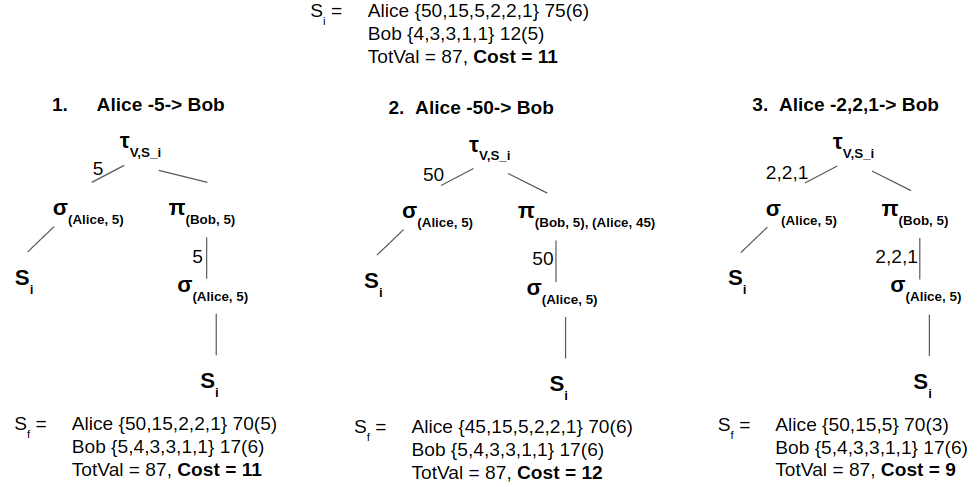
\includegraphics[width=1\columnwidth,keepaspectratio]{figures/utxo_growth/3-logical-plans.png}
    \caption{An example of three equivalent transactions that transfer 5
    tokens from Alice to Bob but incur different state costs.}
    \label{fig:3-logical-plans}
\end{figure}

\subsubsection{The 2-for-1 Transformation}\label{sec:2-for-1}

We again consider the example where Alice wants to give Bob $5$ coins.
Figure~\ref{fig:4th_logical_plan.png} depicts a fourth, more complex,
equivalent transaction. This transaction consists of two subtransactions (cf.
Definition~\ref{def:subtransaction}), where Alice first gives Bob $17$ coins
and then receives $12$.
When the first transaction is completed, an intermediate state ($S'_i$) is
created, which is then given as input to the second transaction, that produces
the final ledger state $\ledgerState_f$ of cost $3$. Observe that, although
more complex, this transaction minimizes the final ledger state ($72\%$ cost
reduction). Intuitively, this transaction spends all of Alice's outputs with
the first sub-transaction and then does the same for Bob with the second
sub-transaction. Therefore, the optimal cost does not depend on input selection
(like
the 3rd plan of Figure~\ref{fig:3-logical-plans}), but requires the combination
of two transactions that implement a single payment, under a specific
amount ($12$). Definition~\ref{def:2-for-1} provides a formal specification of
the \emph{2-for-1} logical (algebraic) transformation.

\begin{figure}[h!]
    \centering
    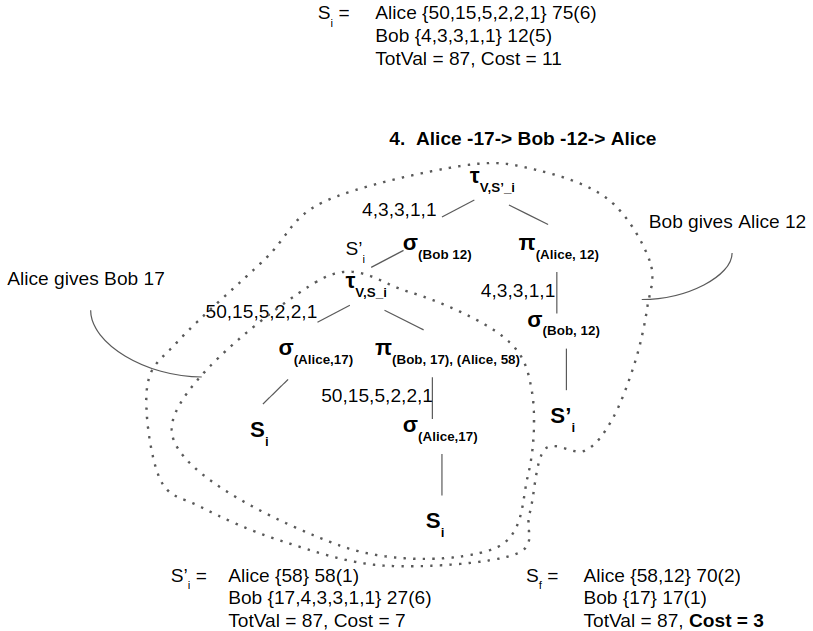
\includegraphics[width=0.9\columnwidth,keepaspectratio]{figures/utxo_growth/4th_logical_plan.png}
    \caption{A 2-for-1 transaction that transfers 5 tokens from Alice to Bob.}
    \label{fig:4th_logical_plan.png}
\end{figure}

\begin{definition}\label{def:2-for-1}
        Given a transaction $\tau_1$, which transfers an amount $V$ from party
        A to B, the algebraic \emph{2-for-1} transformation creates an
        equivalent transaction $\tau_2$, which consists of
        \begin{inparaenum}[(a)]
            \item a subtransaction, which transfers $V+V_c$ from party A to B and
            \item an outer transaction, which transfers $V_c$ from party B to A.
        \end{inparaenum}
\end{definition}

Figure~\ref{fig:2-for-1} depicts the 2-for-1 algebraic transformation based on
an amount $V_c$. To
implement such a scheme we require an \emph{atomic operation}, where the
grouped transactions are executed simultaneously. One method to implement the
atomic transfers is CoinJoin~\cite{coinjoin}, which was proposed for increasing
the privacy in Bitcoin; in CoinJoin, the transaction is constructed and signed
gradually by each party that contributes its inputs. A similar concept is
Algorand's atomic transfers \cite{atomictransfers}, that achieves atomicity by
grouping transactions under a common id.

\begin{figure}[h!]
	\centering
	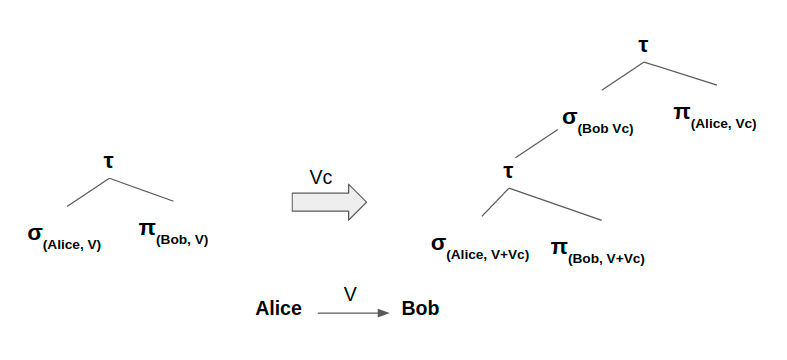
\includegraphics[width=0.9\columnwidth,keepaspectratio]{figures/utxo_growth/2-for-1.png}
	\caption{The 2-for-1 algebraic transformation.}
	\label{fig:2-for-1}
\end{figure}

Intuitively, 2-for-1 reduces the transaction's cost by also consuming UTxOs of
the receiving party, instead of only consuming outputs of the sending party.
Specifically, assume the initial state $\ledgerState_i = \{|A|, |B|\}$, where
$|A|$ denotes the number of outputs owned by party A. When issuing a payment to
B, party A can consume all outputs and consolidate its remaining value to a
single UTxO, the ``change'' output. Such transaction results in state
$\ledgerState_f = \{1, |B|+1 \}$ with cost $cost(\ledgerState_f) = |B|+2$.
If we apply the 2-for-1 transformation, the final state is $\ledgerState_f' =
\{1+1, 1\}$ with a cost of $cost(\ledgerState_f') = 3$; if $|B| > 1$, then
$cost(\ledgerState_f') < cost (\ledgerState_f)$.  Therefore, if the receiving
party has multiple outputs, this transformation creates a transaction with a
smaller cost. Consequently, by giving the opportunity to the receiving party of
a transaction to spend also its outputs, the 2-for-1 transformation
\emph{always} results in a greater shared state cost reduction than the
individual un-transformed transaction in the case where there are no fee
constraints and thus outputs can be spent freely; otherwise it is a cost-based
decision.

\subsubsection{Transaction Total Ordering and the Last-Payer Heuristic Rule}

Assume the following four transactions:
\begin{inparaenum}[(1)]
    \item $T_1$: Alice $\xrightarrow{V_1}$ Charlie,
    \item $T_2$: Bob $\xrightarrow{V_2}$ Charlie,
    \item $T_3$: Eve $\xrightarrow{V_3}$ Alice, and
    \item $T_4$: Eve $\xrightarrow{V_4}$ Bob,
\end{inparaenum}
which are applied on an initial ledger state $\ledgerState_i = \{|Alice| = 5,
|Bob| = 5, |Charlie| = 2, |Eve| = 3\}$ with cost $cost (\ledgerState_i) = 15$;
as before, $|A|$ denotes the number of outputs owned by party A and the state
cost is the number of all UTxOs.

A first execution order is as follows: $T_1 \rightarrow T_2 \rightarrow T_3
\rightarrow T_4$. For simplicity and without loss of the generality, we assume
that when a party pays, it always consumes all available outputs, thus having
with a single output afterwards (the leftover balance). Similarly, when a party
gets paid, the number of UTxOs that it owns increases by one. Next, we describe
the ledger state changes each transaction is executed:
\begin{math}
    \\
    \ledgerState_i = \{|Alice| = 5, |Bob| = 5, |Charlie| = 2, |Eve| = 3\}, cost = 15\\
    T_1: \{|Alice| = 1, |Bob| = 5, |Charlie| = 3, |Eve| = 3\}, cost = 12\\
    T_2: \{|Alice| = 1, |Bob| = 1, |Charlie| = 4, |Eve| = 3\}, cost = 8\\
    T_3: \{|Alice| = 2, |Bob| = 1, |Charlie| = 4, |Eve| = 1\}, cost = 8\\
    T_4: \{|Alice| = 2, |Bob| = 2, |Charlie| = 4, |Eve| = 1\}, cost = 9\\
\end{math}

Assuming a different order, $T_3 \rightarrow T_4 \rightarrow T_1
\rightarrow T_2$, the state changes as follows:

\begin{math}
	\\
	\ledgerState_i = \{|Alice| = 5, |Bob| = 5, |Charlie| = 2, |Eve| = 3\}, cost
	= 15\\
	T_3: \{|Alice| = 6, |Bob| = 5, |Charlie| = 2, |Eve| = 1\}, cost = 14\\
	T_4: \{|Alice| = 6, |Bob| = 6, |Charlie| = 2, |Eve| = 1\}, cost = 15\\
	T_1: \{|Alice| = 1, |Bob| = 6, |Charlie| = 3, |Eve| = 1\}, cost = 11\\
	T_2: \{|Alice| = 1, |Bob| = 1, |Charlie| = 4, |Eve| = 1\}, cost = 7\\
\end{math}

Evidently, the different execution order results in different resulting state
cost. Therefore, by changing the nesting order of the transactions in an
expression tree, different plans may conduct the same payment with different
cost.

Intuitively, parties should have the ability to consume outputs that are
produced by the other transactions. For instance, regarding $T_1$ and $T_3$,
the order $T_3 \rightarrow T_1$ is more cost effective ($cost = 10$) than $T_1
\rightarrow T_3$ ($cost = 11$), since Alice can consume the output created by
Eve. Specifically, if in the last transaction where $\party$ participates,
either as a sender or a receiver, $\party$ is the sender, then it can minimize
its state cost; we call this the \emph{last-payer heuristic rule}.

\subsection{The Transaction Optimization Problem}\label{sec:tx-opt-problem}

Using the above ideas, we now formally define the transaction optimization
problem as a typical \emph{optimization problem}, assuming a set of available
input selection algorithms $\{Sel_1, Sel_2, \dots, Sel_l\}$.

\begin{definition}\label{def:tx-optimization-problem}
    Given $N$ payments between $M$ parties $\party_1, \party_2, \dots, \party_M$ and a
    search space $\mathcal{S}$ of \emph{equivalent} (cf.
    Definition~\ref{def:equiv_total_orders_of_txs}), ordered lists of
    transaction plans that execute the $N$ payments, called \emph{candidate
    solutions}, find the candidate $\tau \in \mathcal{S}$, such that
    $eval(\tau) \leq eval(\rho)$, for all $\rho \in \mathcal{S}$.
    Specifically:
    \begin{enumerate}
        \item A candidate $\rho \in \mathcal{S}$ is an ordered list of
            transaction plans\footnote{We assume that transactions are
            non-correlated (cf. Definition~\ref{def:correlated_tx}) and that all
            orderings are equivalent (cf.
            Definition~\ref{def:equiv_total_orders_of_txs}).} $||T_1||
            \rightarrow
            ||T_2|| \rightarrow \dots \rightarrow ||T_k||$, where the
            transaction plan of
            a transaction $T_x$ is the pair:
            $||T_x|| \defn$ (Logical Expression, Input Selection Algorithm).

        \item The search space $\mathcal{S}$ is defined by all candidates
        $||T_1||
            \rightarrow ||T_2|| \rightarrow \dots \rightarrow ||T_k||$, where,
            for each
            transaction $T_i$, an input selection algorithm from
            $\{Sel_1, Sel_2, \dots, Sel_l\}$ is chosen and, possibly, the 2-for-1 logical
            transformation (cf.  Definition~\ref{def:2-for-1}) is applied.

        \item $eval$ evaluates the cost of every candidate $\rho \in
            \mathcal{S}$ (cf. Definition~\ref{def:tx-cost}) as follows:
            \begin{align*}
                eval : [Transaction] \rightarrow LedgerState \rightarrow Cost,
                \\
                eval([T_1, T_2, \dots, T_k], \ledgerState_{init}) = \\
                cost((txRun(T_k).\ \dots\ .txRun(T_2).txRun(T_1))(\ledgerState_{init})) - cost(\ledgerState_{init})\\
            \end{align*}
            where $cost(S) = |S|$ is the size of a ledger state (cf.
            Definition~\ref{def:lstate}) and the functions $(txRun(T_k).\ \dots\
            .txRun(T_2).txRun(T_1))(\ledgerState_{init})$ output the final
            state after the list of ordered transactions is executed on the
            initial state $\ledgerState_{init}$, according to each individual
            transaction plan $||T_i||$.
    \end{enumerate}
\end{definition}

\paragraph{Solving the Transaction Optimization Problem}

We now present a 3-step, dynamic programming algorithm, which solves the
transaction optimization problem via an exhaustive search and
dynamically pruning candidate solutions:
\begin{enumerate}
    \item Create $N$ transactions $T_{ij}$, $i,j \in [1,M]$,
        corresponding to the payments ($\party_i \xrightarrow[]{V_{ij}} \party_j$),
        as follows:
        \begin{equation*}
            T_{ij} = (\sigma_{\party_i, V_{ij}}(\ledgerState_{init})) \infixOperator (\pi_{\party_j,V{ij}}(\ledgerState_{init}))
        \end{equation*}
        where $V_{ij}$ is the amount to be paid from $\party_i$ to $\party_j$.
        For each $T_{ij}$, find the input selection algorithm in
        $\{Sel_1, Sel_2, \dots, Sel_l\}$ that minimizes $eval(T_{ij},
        \ledgerState_{init})$. Then, enforce the \emph{heuristic rule} to
        create a \emph{single} output per recipient address for each
        transaction.
        At the end of this step, the algorithm outputs $N$ transaction plans,
        \ie $N$ pairs of transaction's $T_{ij}$ logical expression and the
        chosen
        input selection algorithm:
        \begin{equation*}
            ||T_{ij}|| = ((\sigma_{\party_i, V_{ij}}(\ledgerState_{init})) \infixOperator (\pi_{\party_j,V{ij}}(\ledgerState_{init})),\; Sel_s)
        \end{equation*}

    \item On each transaction plan output of Step 1, perform a 2-for-1
        transformation (cf. Definition~\ref{def:2-for-1}). This step produces a
        transformed transaction as
        depicted in Figure~\ref{fig:search_alg_2-for-1}, based on an amount
        $p\times V_{ij}$, where $p$ is a
        configuration parameter of the algorithm, typically in the range $0 < p
        \leq 1$.
        Then, for each of the two transactions that comprise the 2-for-1
        transformation, choose the input selection algorithm that minimizes the
        $eval$ function and enforce the heuristic rule of a \emph{single}
        output per recipient address.  Finally, accept the 2-for-1 transformed
        transaction only if its cost (given by $eval$) is smaller than the
        non-transformed transaction.

        \begin{figure}[h!] %[H]
                \centering
                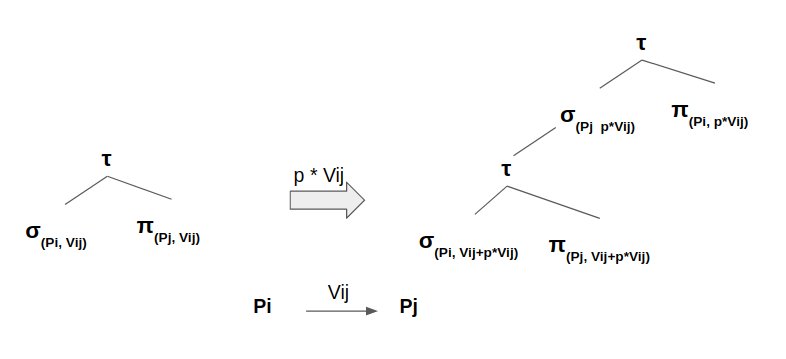
\includegraphics[width=0.8\columnwidth,keepaspectratio]{figures/utxo_growth/search_alg_2-for-1.png}
                \caption{Applying the 2-for-1 transformation to each separate
                transaction.}
                \label{fig:search_alg_2-for-1}
        \end{figure}

        At the end of this step, the algorithm outputs $k$ transaction plans,
        $k \geq N$, comprising of the 2-for-1 transformed and the
        non-transformed transactions, along with their input selection
        algorithms. Importantly, at this point, the algorithm has an optimal
        plan for each \emph{individual} payment ($\party_i
        \xrightarrow[]{V_{ij}} \party_j$), based on an exhaustive search of
        solutions and cost-driven choices.

    \item In this step, the algorithm finds the optimal total order to
        execute the $k$ transactions produced on Step 2. Since there exist $k!$
        permutations, the search space is pruned using the
        \emph{Last-Payer heuristic rule} (cf.
        Section~\ref{sec:tx_optimization_techniques}).
        At the end of this step, the algorithm outputs a totally ordered set of
        transaction plans that solve the optimization problem, \ie executes the
        $N$ payments with a minimum state ledger cost.
\end{enumerate}

Our algorithm's \emph{asymptotic time complexity} depends on its slowest
element.  For simplicity, we assume that applying a transaction on a ledger
state requires constant time. Therefore, in Step 1, creating each of the $N$
transactions is $O(1)$. However, each of the $l$ input selection algorithms may
have different complexity when parsing the $n$ UTxO inputs. For
example,~\cite{karakostas2021efficient} shows that to minimize ``change'', \ie
to find inputs that exactly match the payment's output, requires solving a
Knapsack problem, \ie $O(2^n)$, but is not necessarily state efficient;
instead, the paper proposes an input selection algorithm with complexity $O(n
\log n)$. Step 2 has the same asymptotic complexity as Step 1, as performing
the 2-for-1 transformation requires $O(1)$, as does the application of
heuristics, while choosing an input selection algorithm is the same as in Step
1. Finally, Step 3 requires $O(N!)$, in the corner case when the heuristics do
not prune the search space at all.

On the whole, assuming the complexity of the least efficient input selection
algorithm is $O(\lambda(n)$, our algorithms complexity is $O(\lambda(n) + N!)$,
where $n$ are the available inputs and $N$ is the number of payments.
Theoretically speaking, this is a rather inefficient solution. In practice
though, the wallets of regular users do not control many UTxOs, so $n$ is
expectedly low. The same holds for $N$, as regular users are not expected to
perform complex payments towards multiple third parties.  Nonetheless,
optimizing the employed modules, \eg designing more efficient input selection
algorithms and heuristics, offers an interesting path for future research.

Regarding \emph{optimality}, the transaction plans produced in Step 2 are
optimal \wrt executing the individual transactions, since the algorithm
performs an exhaustive search for the minimum-cost solution. In Step 3, the
algorithm is based on a heuristic rule (Last-Payer) to search for the optimal
total order in a pruned (and thus manageable) space.  Future work will evaluate
the efficiency of this heuristic rule, \ie how well it approximates the optimal
solution, and explore further rules for achieving optimality.

\section{State Efficiency in Bitcoin}\label{sec:fee_model}

We now define the \emph{state efficiency} property. Our goal is to incentivize
users to minimize the global state, without impacting the system's
functionality. In that case, if all users are rational, \ie operate following
the incentives, then the state will be minimized as much as possible. Future
work will explore the actual impact of deploying such incentives in real-world
systems.

To achieve state efficiency, a transaction's fee should be proportional to the
incurred state cost. In other words, the more a transaction increases the
ledger's state, the higher its fees should be. Specifically, a transaction's
fee should reflect:
\begin{inparaenum}[i)]
    \item the transaction's size, \ie the cost of storing a transaction
        permanently on the ledger and
    \item the transaction's state cost.
\end{inparaenum}
A distributed ledger's fee model should aim at incentivizing users
to minimizing both storage types, \ie the distributed ledger and the global
state.

First, we define the \emph{fee function} $\feeFunction$, \ie the function that
assigns an (integer) fee on a transaction, given a ledger state:
$\feeFunction: \mathit{Transaction} \rightarrow \mathit{LedgerState} \rightarrow \mathit{Int}$.
Following, Definition~\ref{def:state-efficiency} describes \emph{state
efficiency}. This property instructs the fee function to (monotonically)
increase fees, if a transaction increases the state. Intuitively, between two
equivalent transactions, the transaction that incurs greater state cost should
also incur a larger fee.

\begin{definition}\label{def:state-efficiency}
    A fee function $\feeFunction$ is \emph{state efficient} if
    \begin{align*}
        \forall \ledgerState \in \ledgerStateSet \forall \tx_1, \tx_2 \in \txSet \mid \tx_1 \equiv \tx_2 \land \mathit{costTx}(\tx_1, \ledgerState) > \mathit{costTx}(\tx_2, \ledgerState):
        \feeFunction(\tx_1, \ledgerState) > \feeFunction(\tx_2, \ledgerState)
    \end{align*}
    for transaction cost function (cf. Definition~\ref{def:tx-cost}) and
    equivalence (cf. Definition~\ref{def:equiv_txs}).
\end{definition}

Evidently, if the utility of users is to minimize transaction fees, a state
efficient fee function ensures that they are also incentivized to minimize the
global state. Finally, Definition~\ref{def:state-efficiency-same-out} sets
\emph{narrow state efficiency}, a special case of state efficiency which
compares equivalent transactions that differ only in their inputs.

\begin{definition}\label{def:state-efficiency-same-out}
    A fee function $\feeFunction$ is \emph{narrow state efficient} if
    \begin{align*}
        \forall \ledgerState \in \ledgerStateSet \forall \tx_1, \tx_2 \in \txSet \mid \\
        \tx_1 \equiv \tx_2 \land \tx_1.\mathsf{outputs} = \tx_2.\mathsf{outputs} \land \mathit{costTx}(\tx_1, \ledgerState) > \mathit{costTx}(\tx_2, \ledgerState): \\
        \feeFunction(\tx_1, \ledgerState) > \feeFunction(\tx_2, \ledgerState)
    \end{align*}
    for transaction cost function (cf. Definition~\ref{def:tx-cost}) and
    equivalence (cf. Definition~\ref{def:equiv_txs}).
\end{definition}

\paragraph{Bitcoin's State Management}\label{sec:bitcoin-fees}
Bitcoin's consensus model does not consider fees. Specifically, the user
decides a transaction's fees and the miners choose whether to include a
transaction in a block. Therefore, it has been stipulated that the level of
fees is the balance between the rational choices of miners, who supply the
market with block space, and users, who demand part of said
space~\cite{bitcoin-fees}.

In practice, users follow the client software's choice even when not
needed~\cite{FCW:MosBoh15}, \eg when blocks are not full. Similarly, miners
usually follow the hard-coded software rules and may accept even zero-fee
transactions. The reference rules of the Bitcoin Wiki~\cite{bitcoin-fees}
define the \emph{fee rate} $x$, which is the fraction of fees per transaction
size, Miners sort transactions based on this metric and solve the Knapsack
problem to fill a new block with transactions that maximize it. Some notable
alternatives also focus on fee
rate~\cite{santos2019miner,rizun2015transaction}, while reference
rules~\cite{bitcoin-fees} used to also take into account the UTxO age.

As before, a transaction consists of inputs and outputs, \ie old UTxOs which
are spent and newly-created UTxOs. Inputs and UTxOs have a fixed size
$\txInputSize$ and $\utxoSize$ respectively.\footnote{This assumption slightly
diverges from the real-world, where UTxOs are typically of varying size
depending on the operations in the ScriptPubKey.} The size of a transaction is
the sum of its inputs and outputs, \ie is a linear combination of
$\txInputSize$ and $\utxoSize$, while a transaction's cost is the difference
between the number of its UTxOs minus its inputs.
Bitcoin's fee function is $\feeFunction = \sizeByteFee \cdot
\mathsf{size}(\tx)$, where $\mathsf{size}(\tx)$ is $\tx$'s size in bytes and
$\sizeByteFee$ is a fixed fee per byte.\footnote{$\sizeByteFee = 0.0067$\$/byte
[September 2020] (\url{https://bitinfocharts.com})}

We break the fee efficiency of $\feeFunction$ via a counterexample. Assume two
transactions which are applied on the same ledger state $\ledgerState$; for
ease of notation, in the rest of the section $\feeFunction(\tx)$ denotes
$\feeFunction(\tx, \ledgerState)$. First, $\tx_1$ has $1$ input and $1$ output,
so its state cost is $\costFunc(\tx_1, \ledgerState) = 0$ and its fee is
$\feeFunction(\tx_1) = \sizeByteFee \cdot (\txInputSize + \utxoSize)$. Second,
$\tx_2$ has $2$ inputs and $1$ output, \ie its state cost is $\costFunc(\tx_2,
\ledgerState) = -1$, since it decreases the state; however, its fee is
$\feeFunction(\tx_2) = \sizeByteFee \cdot (2 \cdot \txInputSize + \utxoSize) =
\feeFunction(\tx_1) + \sizeByteFee \cdot \txInputSize$.  Thus, although
$\costFunc(\tx_1) > \costFunc(\tx_2)$, $\tx_2$'s fee is higher, since it is
larger.

A better alternative fee function is the following:
$\feeFunction' = \sizeByteFee \cdot
\mathsf{size}(\tx) + \utxoFee \cdot \costFunc(\tx, \ledgerState)$.
Note that this is state-efficient in our model  for a
sufficiently small value of $\beta$ (cf. Section~\ref{sec:state-efficient-bitcoin}).
Observe with this function, when
increasing the UTxO set, a user needs to pay an extra fee $\utxoFee$ per UTxO.
Given this change, the reference rules are updated so that, instead of the fee rate, miners use the scoring function:
$\mathsf{score}(\tx) = \frac{\mathsf{fees}(\tx) - \utxoFee \cdot \costFunc(\tx,
\ledgerState)}{\mathsf{size}(\tx)}$, where $\mathsf{fees}(\tx)$ are $\tx$'s
total fees. In market prices, $1$ byte of RAM
costs approximately $\$3.35 \cdot 10^{-9}$~\cite{ram-price}. The average size of a Bitcoin
UTxO is $61$ Bytes~\cite{FCW:DPNH18}, so a single Bitcoin UTxO costs
$\utxoFee = 61 \cdot 3.35 \cdot 10^{-9} = \$2 \cdot 10^{-7}$. Given $10000$
full nodes\footnote{\url{https://bitnodes.io} [July 2020]}, which maintain the
ledger and keep the UTxO in memory, the cost becomes $\utxoFee =
\$0.002$; equivalently, denominated in Bitcoin\footnote{$1 BTC = \$9000$
[\url{https://coinmarketcap.com}; July 2020]}, the cost of creating a UTxO is
$\utxoFee = 22$ satoshi.

This solution incorporates the operational costs of miners, thus it is the
rational choice for miners who aim at maximizing their profit. Observe that,
after subtracting the fees that relate to UTxO costs, the scoring mechanism
behaves the same as the one currently used by Bitcoin miners. Therefore, if
users wish to prioritize their transactions, they would again simply increase
their transaction's fees; in that case, the UTxO portion of the fees (\ie
$\utxoFee \cdot \costFunc(\tx, \ledgerState)$) remains the same, hence higher
$\mathsf{fees}$ result in a higher $\mathsf{score}$, similar to the existing
mechanism. Also we note that this mechanism is directly enforceable on Bitcoin
without the need of a fork.

\subsection{A State Efficient Bitcoin}\label{sec:state-efficient-bitcoin}

Intuitively, to make $\feeFunction$ state efficient we force the creator of
a UTxO to subsidize its consumption, \ie to pay the user who later
consumes it. Our fee function is again: $\feeFunction' =
\sizeByteFee \cdot \mathsf{size}(\tx) + \utxoFee \cdot \costFunc(\tx,
\ledgerState)$. Assume two transactions $\tx_1, \tx_2$ with $i_1, i_2$
inputs and $o_1, o_2$ outputs respectively:
\begin{align}
    \costFunc(\tx_1) > \costFunc(\tx_2) \Leftrightarrow
    o_1 - i_1 > o_2 - i_2 \Leftrightarrow
    o_2 - o_1 < i_2 - i_1 \label{eq:tx-cost-diff}
\end{align}
$\feeFunction'$ is state efficient (cf.
Definition~\ref{def:state-efficiency}) if:
\begin{align}
    \feeFunction'(\tx_1) > \feeFunction'(\tx_2) \Rightarrow \nonumber \\
    \mathsf{size}(\tx_1) \cdot \sizeByteFee + \costFunc(\tx_1) \cdot \utxoFee > \mathsf{size}(\tx_2) \cdot \sizeByteFee + \costFunc(\tx_2) \cdot \utxoFee \Rightarrow \nonumber \\
    (i_1 \cdot \txInputSize + o_1 \cdot \utxoSize) \cdot \sizeByteFee + (o_1 - i_1) \cdot \utxoFee > (i_2 \cdot \txInputSize + o_2 \cdot \utxoSize) \cdot \sizeByteFee + (o_2 - i_2) \cdot \utxoFee \Rightarrow \nonumber \\
     (o_1 - i_1) \cdot \utxoFee - (o_2 - i_2) \cdot \utxoFee > (i_2 \cdot \txInputSize + o_2 \cdot \utxoSize) \cdot \sizeByteFee - (i_1 \cdot \txInputSize + o_1 \cdot \utxoSize) \cdot \sizeByteFee \Rightarrow \nonumber \\
     (i_2 - i_1 + o_1 - o_2) \cdot \utxoFee > ((i_2 - i_1) \cdot \txInputSize + (o_2 - o_1) \cdot \utxoSize) \cdot \sizeByteFee \xRightarrow{(\ref{eq:tx-cost-diff})} \nonumber \\
    \utxoFee > \frac{(i_2 - i_1) \cdot \txInputSize + (o_2 - o_1) \cdot \utxoSize}{(i_2 - i_1) - (o_2 - o_1)} \cdot \sizeByteFee \label{eq:state-efficiency}
\end{align}
If $\feeFunction'$ is narrow state efficient, then $o_1 = o_2$ and the inequality is simplified:
\begin{align}
    \utxoFee > \txInputSize \cdot \sizeByteFee \label{eq:narrow-state-efficiency}
\end{align}

We turn again to the previous example. For transaction $\tx_1$, with $1$ input
and $1$ output, $\feeFunction'(\tx_1) = (\txInputSize + \utxoSize) \cdot
\sizeByteFee$ and for transaction $\tx_2$, with $2$ inputs and $1$ output,
$\feeFunction'(\tx_2) = (2 \cdot \txInputSize + \utxoSize) \cdot \sizeByteFee -
\utxoFee = \feeFunction'(\tx_1) + \sizeByteFee \cdot \txInputSize - \utxoFee$.
Since Inequalities~\ref{eq:state-efficiency}
and~\ref{eq:narrow-state-efficiency} ensure that $\utxoFee > \txInputSize \cdot
\sizeByteFee$, the size fee of the extra input in $\tx_2$ is offset by the
extra fee $\utxoFee$, which is paid by the user who creates it.
Again to evaluate these variables we consider market prices. The size of a
typical, pay-to-script-hash or pay-to-public-key-hash, UTxO is
$34$ Bytes~\cite{btc-tx}, while the size of consuming it is $146$ bytes.
Therefore, to make and make present-day Bitcoin (narrow) state efficient, we can
set $\utxoSize = 34$, $\txInputSize = 146$, $\sizeByteFee = 0.0067$\$, and thus
$\utxoFee > 0.0978$\$.

However, this approach presents a number of challenges. To enforce
$\feeFunction'$, the fee policy should be incorporated in the consensus
protocol and a transaction's validity will depend on its amount of fees. As
long as $\feeFunction'(\tx) > 0$, \ie a transaction cannot have negative fees,
the fee function can be enforced via a \emph{soft} fork. Specifically, this
change is backwards compatible, as miners that do not adopt this change will
still accept transactions that follow the new fee scheme. However, if
$\costFunc(\tx) \ll 0$ and possibly $\feeFunction'(\tx) < 0$, to implement
$\feeFunction'$ we need to establish a ``pot'' of fees. When a user creates
$\tx$ with fee $\feeFunction' = \sizeByteFee \cdot \mathsf{size}(\tx) +
\utxoFee \cdot \costFunc(\tx, \ledgerState)$, the first part ($\sizeByteFee
\cdot \mathsf{size}(\tx)$) is awarded to the miners as before. The second part
($\utxoFee \cdot \costFunc(\tx, \ledgerState)$) is deposited to (or, in case of
negative cost, withdrawn from) the pot. In case of negative cost, the
transaction defines a special UTxO for receiving the reimbursement. At any
point in time, the size of the pot is directly proportional to the UTxO set.
Observe that the miners receive the same rewards as before, so their business
model is not affected by this change. Finally, the cost of flooding the system
with UTxOs increases by $\utxoFee$ per UTxO which, depending on $\utxoFee$, can
render attacks ineffective.


\chapter{
    Blockchain Nash Dynamics
}\label{chap:compliance}

With the advent of Bitcoin~\cite{nakamoto2008bitcoin} the economic aspects of
consensus protocols came to the forefront. While classical literature in
consensus primarily dealt with ``error models'', such as fail-stop or Byzantine
\cite{DBLP:journals/jacm/PeaseSL80}, the pressing question post-Bitcoin is
whether the incentives of the participants align with what the consensus
protocol asks them to do.

Motivated by this, existing literature pursued various research paths.
One line of work investigated
whether the Bitcoin protocol is an equilibrium under certain conditions
\cite{KrollDaveyFeltenWEIS2013,kiayias16EC}. Another, pinpointed protocol
deviations that can be more profitable for some players, assuming others follow
the protocol~\cite{FC:EyaSir14,FC:SapSomZoh16,FCW:JLGVM14,CCS:CKWN16}.
Some works proposed tweaks towards improving the underlying blockchain protocol
in various settings~\cite{FC:FKORVW19,koutsoupias19www}, game-theoretic studies
of pooling behavior~\cite{lewenberg15,CCS:CKWN16,ITCS:ArnWei19}, as well as
equilibria involving abstaining from the protocol~\cite{DBLP:conf/ec/FiatKKP19}
in high cost scenaria. Going beyond consensus, economic mechanisms have also
been considered in the context of multi-party
computation~\cite{CCS:KumMorBen15,FC:DavDowLar19,FC:DavDowLar18}, to
disincentivize ``cheating''.
Finally, a large body of research was dedicated to
optimizing particular attacks; respresentative works
\begin{inparaenum}[i)]
    \item identify optimal selfish mining strategies~\cite{FC:SapSomZoh16};
    \item propose a framework~\cite{CCS:GKWGRC16} for quantitatively
    evaluating blockchain parameters and identifies optimal strategies for
    selfish mining and double-spending, taking into account network delays;
    \item propose alternative strategies~\cite{EPRINT:NKMS15}, that are more
        profitable than selfish mining.
\end{inparaenum}

Though the above works provide some glimpses on how Bitcoin and related
protocols behave from a game-theoretic perspective, they still offer very
little guidance on how to design new consensus protocols. This is a problem of
high importance, given the current negative light shed on Bitcoin's perceived
energy inefficiency and carbon footprint~\cite{martin2021energy} that
asks for alternative protocols. Proof-of-Stake (PoS) ledgers is currently the
most prominent alternative to Bitcoin's Proof-of-Work (PoW) mechanism. While
PoW requires computational effort to produce valid messages, \ie blocks which
are acceptable by the protocol, PoS relies on each party's stake, \ie the
assets they own, and each block is created at (virtually) no cost.
Interestingly, while it is proven that PoS protocols are Byzantine resilient
\cite{C:KRDO17,EPRINT:CGMV18,EPRINT:GHMVZ17,buterin2017casper} and are even
equilibriums under certain conditions \cite{C:KRDO17}, their security is
heavily contested by proponents of PoW protocols via an economic argument. In
particular, the argument termed the \emph{nothing-at-stake}
attack~\cite{li2017securing,ethereumFaq,nothing-at-stake-1} asserts that
parties who maintain a PoS ledger will opt to produce conflicting blocks,
whenever possible, to maximize their expected rewards.

What merit do these criticisms have?  Participating in a blockchain protocol is
a voluntary action that involves a participant downloading the software,
committing some resources, and running the software. Furthermore, especially
given the open source nature of these protocols, nothing prevents the
participant from modifying the behaviour of the software in some way and engage
with the other parties following a modified strategy. There are a number of
adjustments that a participant can do which are undesirable, \eg
\begin{inparaenum}[i)]
    \item run the protocol intermittently instead of continuously;
    \item not extend the most recent ledger of transactions they are aware of;
    \item extend simultaneously more than one ledger of transactions.
\end{inparaenum}
One can consider the above as fundamental {\em infractions} to the protocol
rules and they may have serious security implications, both in terms of the
consistency and the liveness of the underlying ledger.

To address these issues, many blockchain systems introduce additional
mechanisms on top of Bitcoin incentives, frequently with only rudimentary game
theoretic analysis. These include:
\begin{inparaenum}[i)]
    \item rewards for ``uncle blocks'' in Ethereum;
    \item stake delegation~\cite{eosWhitepaper}  in Eos and Polkadot, where
    users assign their participation rights to delegates, as well as stake
    pools in Cardano \cite{SCN:KarKiaLar20};
    \item penalties~\cite{buterin2017casper,casper-incentives} for misbehavior
    in Ethereum 2.0, that enforce forfeiture of large deposits (referred to as
    \emph{``slashing''}) if a party misbehaves, in the sense of being offline
    or using their cryptographic keys improperly.
\end{inparaenum}
The lack of thorough analysis of these mechanisms is of course a serious
impediment to the wider adoption of these systems.

For instance, forfeiting funds may happen inadvertently, due to server
misconfiguration or software and hardware bugs~\cite{khatri2021slashed}.
A party that employs a redundant configuration with multiple replicas, to
increase its crash-fault tolerance, may produce conflicting blocks if, due to a
faulty configuration or failover mechanism, two replicas come alive
simultaneously.  Similarly, if a party employs no failover mechanism and
experiences network connectivity issues, it may fail to participate. Finally,
software or hardware bugs can always compromise an -- otherwise safe and secure
-- configuration.  This highlights the flip side of such penalty mechanisms:
participants may choose to not engage, (\eg to avoid the risk of forfeiting
funds, or because they do not own sufficient funds to make a deposit), or, if
they do engage, they may steer clear of fault-tolerant sysadmin practices, such
as employing a failover replica, which could pose quality of service concerns
and hurt the system in the long run.

The above considerations put forth the fundamental question that motivates our
work: {\em How effective are blockchain protocol designs in disincentivizing
particular infractions?} In more detail, the question we ask is whether selfish
behavior can lead to deviations, starting with a given blockchain protocol as
the initial point of reference of honest --- compliant --- behavior.

\subsection*{Contributions}
Our main question relates to the Nash-dynamics of blockchain
protocols. In the classical Nash-dynamics problem~\cite{rosenthal73}, the
question is whether selfish players performing step-wise payoff improving moves
lead the system to an equilibrium, and in how many steps this may happen; \eg
\cite{DBLP:conf/stoc/FabrikantPT04} provides an important case of congestion
games. In this perspective, the action space can be seen as a directed graph,
with vertices representing vectors of player strategies and edges corresponding
to player moves.

In this work, we adapt Nash dynamics to the setting of blockchain protocols,
with a particular focus on the study of specific undesirable protocol
infractions.  Importantly, instead of asking for convergence, we ask whether
the ``cone'' in the directed graph positioned at the protocol contains any
strategies that belong to a given set of infractions $\infractionPredicate$
(cf. Figure~\ref{fig:cone}). If the cone is free of infractions, then the
protocol is said to be $\infractionPredicate$-compliant. Motivated by Chien and
Sinclair \cite{DBLP:journals/geb/ChienS11}, we consider
$\epsilon$-Nash-dynamics, \ie considering only steps in the graph that improve
the participant payoff more than $\epsilon$. Armed with this model, we
investigate a number of protocols, both in the PoW and PoS setting, from a
compliance perspective.
Notably, we provide indicative values for $\epsilon$,
beyond which a protocol is not compliant. Nonetheless, our work is
complimentary to research that investigates optimality of particular attacks;
specifically, these works could be used in conjunction with our model to
provide tighter, if not optimal, bounds on $\epsilon$.

\begin{figure}[h]
    \begin{center}
        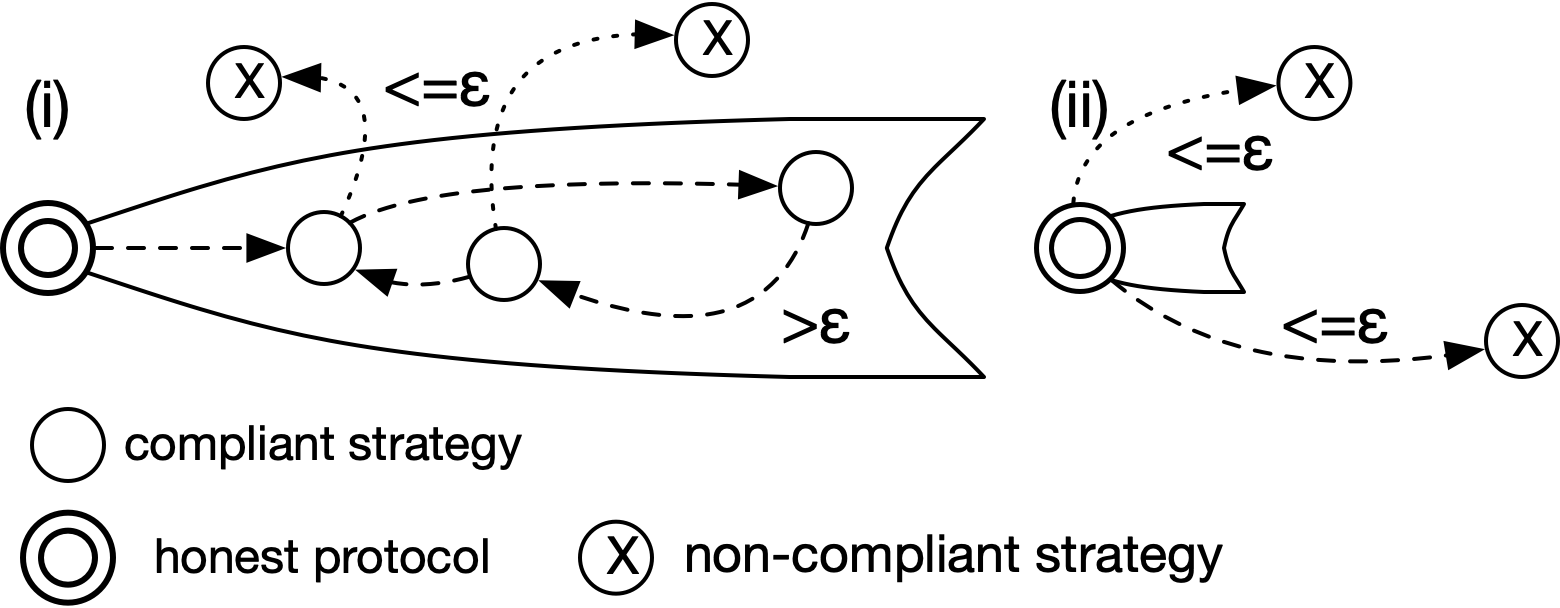
\includegraphics[width=0.8\columnwidth]{figures/compliance/cone.png}
    \end{center}
    \caption{
        Illustration of a compliant protocol that does not exhibit an
        equilibrium (i), vs a protocol which is an approximate Nash equilibrium
        (ii).
    }
    \label{fig:cone}
\end{figure}

First, Section~\ref{sec:model} describes our model of \emph{compliant}
strategies and protocols. A strategy is compliant if a party that employs it
never violates a predicate $\infractionPredicate$, which captures well-defined
types of deviant behavior. Accordingly, a protocol is compliant if, assuming a
starting point where no party deviates, no party will eventually employ a
non-compliant strategy, assuming sequential unilateral defections.
Section~\ref{sec:blockchains} specifies compliance for blockchain protocols,
under an infraction predicate that captures abstaining and producing
conflicting blocks, and two types of utility, absolute rewards and profit.
Following, we explore different reward schemes and families of protocols.
First, Section~\ref{sec:universal} shows that \emph{fair} rewards, \ie which
depend only on a party's mining or staking power, result in compliance \wrt
rewards alone (i.e., when costs are negligible), but non-compliance \wrt profit
(rewards minus costs). Next, we explore block-proportional rewards, \ie which
depend on the blocks adopted by an impartial observer of the system.
Section~\ref{subsec:bitcoin} shows that PoW systems are compliant \wrt rewards.
Section~\ref{subsec:single-leader-pos} shows that PoS systems, which enforce
that a single party participates at a time, are compliant, under a synchronous
network, but non-compliant under a lossy network.
Section~\ref{subsec:multi-leader-pos} shows that PoS systems, which allow
multiple parties to produce blocks for the same time slot, are not compliant.
Notably, our negative results show that a party can gain a
\emph{non-negligible} reward by being non-compliant. Finally, we evaluate
compliance under various externalities, \ie an exchange rate, which models
real-world prices, and external rewards, which come as a result of successful
attacks. We show that, historically, the market's response is not sufficient to
disincentivize attacks, so penalties should be necessary, for the level of
which we provide estimations based on the ledger's parameters and the market's
expected behavior.

\section{The Setting}

We consider a distributed protocol $\proto$, which is executed by all parties in
a set $\partySet$, and which is performed over a number of time slots. Our
analysis is restricted on executions where every party $\party \in \partySet$
is activated on each time slot. The activation is scheduled by an environment
$\env$, which also provides the parties with inputs.

We use $\secparam$ to denote $\proto$'s security parameter, and
$\mathsf{negl}(\cdot)$ to denote that a function is negligible, i.e.,
asymptotically smaller than the inverse of any polynomial. By $[n]$, we denote
the set $\{1,\ldots,n\}$. The expectation of a random variable $X$ is denoted
by $E[X]$.

\subsection{Network Model}\label{sec:network-model}

We assume a peer-to-peer network. Specifically, parties do not communicate via
point-to-point connections, but rather use a variant of the \emph{diffuse}
functionality defined in~\cite{EC:GarKiaLeo15}, described as follows.

\paragraph{Diffuse Functionality}\label{par:diffuse}
The functionality initializes a variable $\emph{slot}$ to $1$, which is
readable from all parties. In addition, it maintains a string
$\textsc{Receive}_{\party}()$ for each party $\party$. Each party $\party$ is
allowed to fetch the contents of $\textsc{Receive}_{\party}()$ at the beginning
of each time slot. To diffuse a (possibly empty) message $\mesg$, $\party$
sends to the functionality $\mesg$ and an integer index $i_\mesg$, which
indicates the message delivery priority of $\mesg$ (see below). In turn,
the functionality records $\mesg$ and $i_\mesg$. On each slot, every party completes its
activity by sending a special $\textsc{Complete}$ message to the functionality.
When all parties submit $\textsc{Complete}$, the functionality delivers the
messages, which are diffused during this slot, as follows.  First, it groups
all messages based on their associated index and sorts them, with messages with
smaller index having higher priority. Then, it randomizes the order of each
group's messages, \ie which are associated with the same index.  Therefore,
eventually all messages are sorted in a well-defined order.  Subsequently, the
functionality includes all messages in the $\textsc{Receive}_{\party}()$ string
of every party $\party \in \partySet$, following the aforementioned order.
Hence, all parties receive all diffused messages, without any information
on each message's creator. Finally, the functionality increases the value of $\emph{slot}$
by $1$.

\paragraph{Lossy Diffuse Functionality}\label{sec:lossy-network}
The lossy diffuse functionality is similar to the above variant, with one
difference: it is parameterized with a probability $\networkLossProb$, which
defines the probability that a message $\mesg$ is dropped, \ie it is not
delivered to any recipient. This functionality aims to model the setting where
a network with stochastic delays is used by an application, where users reject
messages which are delivered with delay above a (protocol-specific) limit. For
example, various protocols, like Bitcoin~\cite{nakamoto2008bitcoin}, resolve
message conflicts based on the order of delivery; thus, delaying a message for
long enough, such that a competing message is delivered beforehand, is
equivalent to dropping the message altogether.

\subsection{Approximate Nash Equilibrium}\label{sec:equilibrium}

An approximate Nash equilibrium is a common tool for expressing a solution to a
non-cooperative game involving $\totalParties$ parties $\party_1,\ldots,\party_n$. Each party $\party_i$
employs a strategy $\strategy_i$. The strategy is a set of rules and actions
the party makes, depending on what has happened up to any point in the game,
\ie it defines the part of the entire distributed protocol $\proto$ performed
by $\party_i$. There exists an ``honest'' strategy, defined by $\proto$, which
parties may employ; for ease of notation,
$\proto$ denotes both the distributed protocol and the honest strategy.
A \emph{strategy profile} is a vector of all players' strategies.

Each party $\party_i$ has a game \emph{utility} $\utility_i$, which is a real
function that takes as input a strategy profile. A strategy profile is an
$\epsilon$-Nash equilibrium when no party can increase its utility more than
$\epsilon$ by \emph{unilaterally} changing its strategy
(Definition~\ref{def:equilibrium}).

\begin{definition}\label{def:equilibrium}
    Let $\epsilon$ be a non-negative real number and $\strategySet$ be the set of all strategies a party may employ.
    Also let $\profile^* = (\strategy^*_i, \strategy^*_{-i})$ be a strategy profile of
    $\partySet$, where $\strategy^*_i$ is the strategy followed by $\party_i$ and $\strategy^*_{-i}$ denotes the $\totalParties - 1$
    strategies employed by all parties except $\party_i$. We say that
    $\profile^*$ is an \emph{$\epsilon$-Nash equilibrium} \wrt a utility vector $\bar{\utility} = \langle \utility_1, \ldots, \utility_\totalParties \rangle$ if:
    $$\forall \party_i \in \partySet \; \forall \strategy_i \in \strategySet \setminus \{ \strategy^*_i \} : \utility_i(\strategy^*_i, \strategy^*_{-i}) \geq \utility_i(\strategy_i, \strategy^*_{-i}) - \epsilon$$
\end{definition}

\section{Compliance Model}\label{sec:model}

We assume a distributed protocol $\proto$, which is performed by a set of
parties $\partySet$ over a number of time slots.
In our analysis, each party $\party \in \partySet$ is associated with
a number $\miningpower_{\party} \in [0, 1]$. $\miningpower_{\party}$ identifies
$\party$'s percentage of participation power in the protocol, \eg its votes,
hashing power, staking power, \etc; consequently, $\sum_{\party \in \partySet}
\miningpower_{\party} = 1$.

\subsection{Basic Notions}\label{subsec:basic}
A protocol's execution $\execution_{\env, \sigma, \slot}$ at a given time slot
$\slot$ is probabilistic and parameterized by the environment $\env$ and the
strategy profile $\sigma$ of the participating parties. As discussed, $\env$
provides the parties with inputs and schedules their activation. For notation
simplicity, when $\slot$ is omitted, $\execution_{\env, \sigma}$ refers to the
end of the execution, which occurs after polynomially many time slots.

An \emph{execution trace} $\executionTrace_{\env, \sigma, \slot}$ on a time slot
$\slot$ is the value that the random variable $\execution_{\env, \sigma, \slot}$ takes for a fixed
environment $\env$ and strategy profile $\sigma$, and for fixed random coins of
$\env$, each party $\party \in \partySet$, and every
protocol-specific oracle (see below). A party $\party$'s view of an
execution trace $\executionTrace_{\env, \sigma, \slot}^{\party}$ consists of
the messages that $\party$ has sent and received until slot $\slot$. For
notation simplicity, we will omit the subscripts $\{ \env,
\sigma, \slot \}$ from both $\execution$ and $\executionTrace$, unless
required for clarity.\smallskip

The protocol $\proto$ defines two components, which are related to our
analysis: (1) the oracle $\oracle_\proto$, and (2) the ``infraction'' predicate
$\infractionPredicate$. We present these two components below.

\paragraph{The Oracle $\oracle_\proto$}
The oracle $\oracle_\proto$ provides the parties with the core functionality
needed to participate in $\proto$. For example, in a Proof-of-Work (PoW) system
$\oracle_\proto$ is the random or hashing oracle, whereas in an authenticated
Byzantine Agreement protocol $\oracle_\proto$ is a signing oracle. On each time
slot, a party can perform at most a polynomial number of queries to
$\oracle_\proto$; in the simplest case, each party can submit a single query
per slot. Finally, $\oracle_\proto$ is \emph{stateless}, \ie its random coins
are decided upon the beginning of the execution and its responses do not depend
on the order of the queries.

\paragraph{The Infraction Predicate $\infractionPredicate$}
The infraction predicate $\infractionPredicate$ abstracts the
deviant behavior that the analysis aims to capture. Specifically,
$\infractionPredicate$, when given the execution trace and a party $\party$,
responds with $1$ only if $\party$ deviates from the protocol in some
well-defined manner. Definition~\ref{def:infraction-predicate} provides the
core generic property of $\infractionPredicate$, \ie that honest
parties never deviate. For ease of notation, we will next simply write $\infractionPredicate$ unless required for clarity.
With hindsight, our analysis will
focus on infraction predicates that capture either producing conflicting
messages or abstaining from the protocol.

\begin{definition}[Infraction Predicate Property]\label{def:infraction-predicate}
    The infraction predicate $\infractionPredicate$ has the property that, for
    every execution trace $\executionTrace$ and for every party $\party \in
    \partySet$, if $\party$ employs the (honest) strategy $\proto$ then
    $\infractionPredicate(\executionTrace, \party) = 0$.
\end{definition}

We stress that Definition~\ref{def:infraction-predicate} implies that
$\infractionPredicate$ being $0$ is a necessary, but \emph{not} a sufficient
condition, for a party to be honest. Specifically, for all honest parties
$\infractionPredicate$ is always $0$, but $\infractionPredicate$ might
also be $0$ for a party that deviates from $\proto$, in such way that is not
captured by $\infractionPredicate$. In that case, we say that the party employs
an $\compliant$ strategy (Definition~\ref{def:compliant-strategy}). A strategy
profile is $\compliant$ if all of its strategies are $\compliant$; naturally,
the ``all honest'' profile $\profile_\proto$, \ie when all parties employ
$\proto$, is -- by definition -- $\compliant$.

\begin{definition}[Compliant Strategy]\label{def:compliant-strategy}
    Let $\infractionPredicate$ be an infraction predicate. A strategy $\strategy$ is
    \emph{$\mathcal{X}$-compliant} if and only if $\infractionPredicate(\executionTrace, \party) =
    0$ for every party $\party$ and for every trace $\executionTrace$ where $\party$ employs $\strategy$.
\end{definition}

\paragraph{The observer $\observer$}
We assume a special party $\observer$, the \emph{(passive)
observer}. This party does not actively participate in the execution, but it
runs $\proto$ and observes the protocol's execution. Notably, $\observer$ is
\emph{always online}, \ie it bootstraps at the beginning of the execution and
is activated on every slot, in order to receive diffused messages. Therefore,
the observer models a user of the system, who frequently uses the system but
does not actively participate in its maintenance. Additionally, at the last
round of the execution, the environment $\env$ activates only $\observer$, in
order to receive the diffused messages of the penultimate round and have a
complete point of view.

As mentioned in Section~\ref{sec:equilibrium}, we assume a utility $\utility_i$ for every party $\party_i$, so the utility vector defines the payoff values for
each party. In our examples, a party's utility depends on two parameters:
\begin{inparaenum}[i)]
    \item the party's rewards, which are distributed by the protocol, from the
        point of view of $\observer$;
    \item the cost of participation.
\end{inparaenum}

\subsection{Compliant Protocols}\label{subsec:compliant}

To define the notion of an $(\epsilon, \infractionPredicate)$-compliant protocol
$\proto$, we require two parameters:
\begin{inparaenum}[(i)]
    \item the associated infraction predicate $\infractionPredicate$ and
    \item a non-negative real number $\epsilon$.
\end{inparaenum}
Following Definition~\ref{def:compliant-strategy}, $\infractionPredicate$
determines the set of compliant strategies that the parties may follow in
$\proto$. Intuitively, $\epsilon$ specifies the sufficient gain threshold after which a party
switches strategies. In particular, $\epsilon$ is
used to define when a strategy profile $\sigma'$ is \emph{directly reachable}
from a strategy profile $\sigma$, in the sense that $\sigma'$ results from the
unilateral deviation of a party $\party_i$ from $\sigma$ and, by this
deviation, the utility of $\party_i$ increases more than $\epsilon$.
Generally, $\sigma'$ is \emph{reachable} from $\sigma$, if $\sigma'$ results
from a ``path'' of strategy profiles, starting from $\sigma$, which are
sequentially related via direct reachability. Finally, we define the \emph{cone}
of a profile $\sigma$ as the set of all strategies that are
reachable from $\sigma$, including $\sigma$ itself.

Given the above definitions, we say that $\proto$ is
$(\epsilon,\mathcal{X})$-compliant if the cone of the ``all honest'' strategy
profile $\profile_\proto$ contains only profiles that consist of $\compliant$
strategies. Thus, if a protocol is compliant, then the parties may
(unilaterally) deviate from the honest strategy only in a compliant manner, as
dictated by $\infractionPredicate$.

Formally, first we define ``reachability'' between two strategy profiles, as
well as the notion of a ``cone'' of a strategy profile \wrt the reachability
relation, and then we define a compliant protocol \wrt its associated
infraction predicate.

\begin{definition}\label{def:reach}
    Let:
    \begin{inparaenum}[i)]
        \item $\epsilon$ be a non-negative real number;
        \item $\proto$ be a protocol run by parties $\party_1, \ldots, \party_\totalParties$;
        \item $\bar{\utility}=\langle \utility_1, \ldots, \utility_\totalParties \rangle$ be a utility vector, where $\utility_i$ is the utility of $\party_i$;
        \item $\strategySet$ be the set of all strategies a party may employ.
    \end{inparaenum}
    We provide the following definitions.
    \begin{enumerate}
        \item Let $\profile, \profile' \in \strategySet^\totalParties$ be two strategy profiles where $\profile = \langle \strategy_1, \ldots, \strategy_\totalParties \rangle$ and $\profile'= \langle \strategy'_1, \ldots, \strategy'_\totalParties \rangle$. We say that $\profile'$ is \emph{directly $\epsilon$-reachable from $\profile$ \wrt $\bar{\utility}$}, if there exists $i \in [\totalParties]$ \st (i) $\forall j \in [\totalParties] \backslash \{i\}: \strategy_j = \strategy'_j$ and (ii) $\utility_i(\profile') > \utility_i(\profile) + \epsilon$.
        \item Let $\profile, \profile' \in \strategySet^\totalParties$ be two distinct profiles. We say that $\profile'$ is \emph{$\epsilon$-reachable from $\profile$ \wrt $\bar{\utility}$}, if there exist profiles $\profile_1, \ldots, \profile_k$ such that (i) $\profile_1 = \profile$, (ii) $\profile_k = \profile'$, and (iii) $\forall j \in [2, k]$ it holds that $\profile_j$ is directly $\epsilon$-reachable from $\profile_{j-1}$ \wrt $\bar{\utility}$.
        \item For every strategy profile $\profile \in \strategySet^\totalParties$ we define the \emph{$(\epsilon, \bar{\utility})$-cone of $\profile$} as the set:
        \[\mathsf{Cone}_{\epsilon, \bar{\utility}}(\profile) := \{\profile' \in \strategySet^\totalParties\;|\;(\profile' = \profile) \lor (\profile'\mbox{ is $\epsilon$-reachable from }\profile\mbox{ \wrt }\bar{\utility})\}\;.\]
    \end{enumerate}
\end{definition}

\begin{definition}\label{def:compliant}
    Let:
    \begin{inparaenum}[i)]
        \item $\epsilon$ be a non-negative real number;
        \item $\proto$ be a protocol run by the parties $\party_1, \ldots, \party_\totalParties$;
        \item $\infractionPredicate$ be an infraction predicate;
        \item $\bar{\utility}=\langle \utility_1, \ldots, \utility_\totalParties \rangle$ be a utility vector, where $\utility_i$ is the utility of party $\party_i$;
        \item $\strategySet$ be the set of all strategies a party may employ;
        \item $\strategySet_{\infractionPredicate}$ be the set of $\compliant$ strategies.
    \end{inparaenum}

    A strategy profile $\profile \in \strategySet^n$ is $\compliant$ if $\profile \in (\strategySet_{\infractionPredicate})^\totalParties$.

    The \emph{$(\epsilon,\bar{U})$-cone of $\proto$}, denoted by $\mathsf{Cone}_{\epsilon,\bar{U}}(\proto)$, is the set $\mathsf{Cone}_{\epsilon, \bar{\utility}}(\profile_\proto)$, \ie the set of all strategies that are $\epsilon$-reachable from the ``all honest'' strategy profile $\profile_\proto = \langle \proto, \ldots, \proto \rangle$ \wrt $\bar{\utility}$, also including $\profile_\proto$.

    $\proto$ is \emph{$(\epsilon,\mathcal{X})$-compliant \wrt $\bar{\utility}$} if $\mathsf{Cone}_{\epsilon,\bar{U}}(\proto) \subseteq (\strategySet_{\infractionPredicate})^\totalParties$, \ie all strategy profiles in the $(\epsilon,\bar{\utility})$-cone of $\proto$ are $\compliant$.
\end{definition}

Proposition~\ref{prop:eq_comp} shows that Definition~\ref{def:compliant} expresses a relaxation of the standard approximation Nash equilibrium (Definition~\ref{def:equilibrium}).

\begin{proposition}\label{prop:eq_comp}
    Let:
    \begin{inparaenum}[i)]
        \item $\epsilon$ be a non-negative real number;
        \item $\proto$ be a protocol run by the parties $\party_1, \ldots, \party_\totalParties$;
        \item $\infractionPredicate$ be an infraction predicate;
        \item $\bar{\utility}=\langle \utility_1, \ldots, \utility_\totalParties \rangle$ be a utility vector, with $\utility_i$ the utility of $\party_i$.
    \end{inparaenum}
    If $\proto$ is an $\epsilon$-Nash equilibrium \wrt $\bar{\utility}$ (\ie $\profile_\proto=\langle \proto, \ldots, \proto \rangle$ is an $\epsilon$-Nash equilibrium \wrt $\bar{\utility}$), then $\proto$ is $(\epsilon, \infractionPredicate)$-compliant \wrt $\bar{\utility}$.
\end{proposition}
\begin{proof}
Assume that $\profile_\proto$ is an $\epsilon$-Nash equilibrium \wrt $\bar{\utility}$ and let $\profile'=(\strategy'_1, \ldots, \strategy'_\totalParties)$ be a strategy profile. We will show that $\profile'$ is not directly $\epsilon$-reachable from $\profile_\proto$ \wrt $\bar{\utility}$.

Assume that there exists $i \in [\totalParties]$ s.t. $\forall j \in [\totalParties] \backslash\{i\}: \strategy'_j = \proto$. Since $\profile_\proto$ is an $\epsilon$-Nash equilibrium \wrt $\bar{\utility}$, it holds that $\utility_i(\profile') \leq \utility_i(\profile_\proto) + \epsilon$. Therefore, Definition~\ref{def:reach} is not satisfied and $\profile'$ is not directly $\epsilon$-reachable from $\profile_\proto$ \wrt $\bar{\utility}$.

Since no profiles are directly $\epsilon$-reachable from $\profile_\proto$ \wrt $\bar{\utility}$, it is straightforward that there are no $\epsilon$-reachable strategy profiles from $\profile_\proto$ \wrt $\bar{\utility}$. The latter implies that the $(\epsilon, \bar{\utility})$-cone of $\proto$ contains only $\profile_\proto$, \ie $\mathsf{Cone}_{\epsilon,\bar{\utility}}(\proto) = \{ \profile_\proto\}$. By Definitions~\ref{def:infraction-predicate} and~\ref{def:compliant-strategy}, $\profile_\proto$ is $\compliant$, so we deduce that $\proto$ is $(\epsilon,\infractionPredicate)$-compliant \wrt $\bar{\utility}$.
\end{proof}

\section{Blockchain Protocols}\label{sec:blockchains}

In this work, we focus on blockchain-based distributed ledger protocols.  In
the general case, a ledger defines a global state, which is distributed across
multiple parties and is maintained via a consensus protocol. The distributed
ledger protocol defines the validity rules which allow a party to extract the
final ledger from its view. A
blockchain is a distributed database, where each message $\mesg$ is a block
$\block$ of transactions and each transaction updates the system's global
state. Therefore, at any point of the execution, a party $\party$ holds some view of
the global state, which comprises of the blocks that $\party$ has
adopted. We note that, if at least one valid block is diffused (\wrt the
validity rules of the protocol), then every honest party can
extract a final ledger from its execution view.

\subsection{The Setting}\label{subsec:setting}

Every blockchain protocol $\proto$ defines a \emph{message validity} predicate
$\messageValidityPredicate$.  A party $\party$ accepts a block $\block$,
received during a slot $\slot$ of the execution, if it holds that
$\messageValidityPredicate(\executionTrace^{\party}_\slot, \block) = 1$. For
example, in Proof-of-WorK (PoW) systems like
Bitcoin~\cite{nakamoto2008bitcoin}, a block is valid if its hash is below a
certain threshold, while in Proof-of-Stake (PoS) protocols like
Ouroboros~\cite{C:KRDO17}, a block is valid if it has been created by a
specific party, according to a well-known leader schedule. In all cases, a
block $\block$ is valid only if the party that creates it submits a query for
$\block$ to the oracle $\oracle_\proto$ beforehand.

Each block $\block$ is associated with the following metadata:
\begin{inparaenum}[i)]
    \item an index $\mathit{index}(\block)$;
    \item the party $\mathit{creator}(\block)$ that created $\block$;
    \item a set $\mathit{ancestors}(\block) \subseteq
    \executionTrace^{\mathit{creator}(\block)}$, \ie blocks in the view of
    $\mathit{creator}(\block)$ (at the time of $\block$'s creation)
    referenced by $\block$.
\end{inparaenum}

\noindent Message references are implemented as hash pointers, given a hash function
$\hash$ employed by the protocol. Specifically, each block $\block$ contains the
hash of all blocks in the referenced blocks $\mathit{ancestors}(\block)$.
Blockchain systems
are typically bootstrapped via a global common reference string, \ie a
``genesis'' block $\genesis$.
Therefore, the blocks form a hash tree, stemming from $\genesis$.
$\mathit{index}(\block)$ is the height of $\block$ in the hash tree. If
$\block$ references multiple messages, \ie belongs to multiple tree branches,
$\mathit{index}(\block)$ is the height of the longest one.

The protocol also defines the \emph{message equivalency operator}, $\equiv$. Specifically, two messages are equivalent if
their hashes match, \ie $\mesg_1 \equiv \mesg_2 \Leftrightarrow \hash(\mesg_1) =
\hash(\mesg_2)$. At a high level, two equivalent messages are
interchangeable by the protocol.

\paragraph{Infraction Predicate}\label{sec:blockchain-infraction-predicate}
In our analysis of blockchain systems, we consider two types of deviant
behavior (Definition~\ref{def:blockchain-infraction}):
\begin{inparaenum}[i)]
    \item creating conflicting valid messages,
    \item abstaining.
\end{inparaenum}
We choose these predicates because they may lead to non-compliance in
interesting use cases. For the former, conflicting valid messages, \ie chain
forks, are the primary reason for failure to achieve consensus, so exploring
when a party is incentivized to initiate a fork is particularly interesting.
For the latter, increased and continuous participation typically helps the
safety of deployed systems, as motivating more users to participate in a
compliant manner increases the level of power that an adversary needs to reach
in order to break a system's security.

\begin{definition}[Blockchain Infraction Predicate]\label{def:blockchain-infraction}
    Given a party $\party$ and an execution trace $\executionTrace_{\env, \sigma, \slot}$,
    we define the following infraction predicates:
    \begin{enumerate}
        \item
            \emph{conflicting predicate}: $\infractionPredicate_{conf}(\executionTrace_{\env, \sigma, \slot}, \party) = 1$ if
            $\exists \block, \block'
            \in \executionTrace_{\env, \sigma, \slot}:\messageValidityPredicate(\executionTrace_{\env, \sigma, \slot}^{\party}, \block)=\messageValidityPredicate(\executionTrace_{\env, \sigma, \slot}^{\party}, \block')=1\land
            \mathit{index}(\block) = \mathit{index}(\block') \land \block \not \equiv
            \block' \land \mathit{creator}(\block) = \mathit{creator}(\block') = \party$;
        \item
            \emph{abstaining predicate}: $\infractionPredicate_{abs}(\executionTrace_{\env, \sigma, \slot}, \party) = 1$ if
            $\party$ makes \emph{no} queries to the oracle $\oracle_\proto$
            during slot $\slot$;
        \item
            \emph{blockchain predicate}: $\infractionPredicate_{bc}(\executionTrace_{\env, \sigma, \slot}, \party) = 1$ if it holds
            $(\infractionPredicate_{conf}(\executionTrace_{\env, \sigma, \slot}, \party) = 1) \lor (\infractionPredicate_{abs}(\executionTrace_{\env, \sigma, \slot}, \party) = 1)$.
    \end{enumerate}
\end{definition}

\begin{remark*}
Preventing conflicting messages is not the same
as resilience against sybil attacks~\cite{douceur2002sybil}. Sybil resilience
mechanisms restrict an attacker from creating multiple identities, in order to
participate in a distributed system. In comparison, our infraction predicate
ensures that a user does not increase their utility by violating the infraction
conditions for each identity they control. Therefore, a system may be compliant
but not sybil resilient, \eg if a party can participate via multiple identities
but it cannot increase its utility by producing conflicting messages, and vice
versa.
\end{remark*}

Finally, at the end of the execution, the observer $\observer$ outputs a chain
$\chain_{\observer, \executionTrace}$. Typically, this is the longest valid chain, \ie the longest
branch of the tree that stems from genesis $\genesis$.\footnote{For simplicity we assume that the longest chain (in terms of
blocks) also contains the most hashing power, which is the metric used in PoW
systems like Bitcoin.} In case multiple longest chains exist, a choice is made
either at random or following a chronological ordering of messages. The number
of messages in $\chain_{\observer, \executionTrace}$ that are created by a party $\party$ is
denoted by $\msgOutputSet_{\party, \executionTrace}$.

\subsection{Utility: Rewards and Costs}\label{sec:blockchain-utility}

For each execution, the blockchain protocol defines a number of total rewards,
which are distributed among the participating parties. For each party $\party$,
these rewards are expressed via the \emph{reward random variable}
$\reward_{\party, \execution}$.  For a specific trace $\executionTrace$, the
random variable takes a non-negative real value, denoted by $\reward_{\party,
\executionTrace}$. Intuitively, $\reward_{\party, \executionTrace}$ describes
the rewards that $\party$ receives from the protocol from the point of view of
the observer $\observer$, \ie \wrt the blocks accepted by
$\observer$.

Our analysis restricts to systems where rewards are distributed to parties if
and only if the genesis block is extended by at least one block during the
execution, in which case at least one party receives a non-negative amount of
rewards (Assumption~\ref{ass:reward-distribution}).

\begin{assumption}\label{ass:reward-distribution}
    Let $\executionTrace$ be an execution trace. If no block is produced during $\executionTrace$, then it
    holds that $\forall \party \in \partySet: \reward_{\party, \executionTrace} =
    0$.
    If at least one block is produced during $\executionTrace$, then it
    holds that $\exists \party \in \partySet: \reward_{\party, \executionTrace} \neq
    0$.
\end{assumption}

In addition to rewards, a party's utility is affected by cost. Specifically,
the \emph{cost random variable} $\cost_{\party, \execution}$ expresses the
operational cost that $\party$ during an execution $\execution$. For a fixed
trace $\executionTrace$, $\cost_{\party, \executionTrace}$ is a non-negative
real value. Our analysis is restricted to cost schemes which are \emph{linearly
monotonically increasing} in the number of queries that a party makes to the
oracle $\oracle_\proto$, with no queries incurring zero cost
(Assumption~\ref{ass:zero-cost}). Intuitively, this assumption considers the
electricity cost of participation, while the cost of equipment and other
operations, such as parsing or publishing messages, is zero.

\begin{assumption}\label{ass:zero-cost}
    For every execution trace $\executionTrace$, a party $\party$'s cost is
    $\cost_{\party, \executionTrace} = 0$ if and only if it performs no queries
    to $\oracle_\proto$ in every time slot. Else, if during $\executionTrace$ a party $\party$ performs
    $t$ queries, then its cost is $\cost_{\party, \executionTrace} = t \cdot \queryCost$, for some fixed parameter $\queryCost$.
\end{assumption}

Next, we define two types of utility. The first type, \emph{Reward}, considers
the expected rewards that a party receives when the cost is near $0$, while the
second type, \emph{Profit}, considers rewards minus participation cost.

\begin{definition}\label{def:utility}
    Let $\profile$ be a strategy profile and $\execution_\profile$ be an
    execution during which parties follow $\profile$. We define two types of
    blockchain utility $\utility_{\party}$ of a party $\party$ for $\profile$:
    \begin{enumerate}
        \item \emph{Reward}: $\utility_{\party}(\profile) = E[\reward_{\party, \execution_\profile}]$
        \item \emph{Profit}: $\utility_{\party}(\profile) = E[\reward_{\party, \execution_\profile}] - E[\cost_{\party, \execution_\profile}]$
    \end{enumerate}
\end{definition}

For the computation of $\utility_{\party}$, the
environment $\env$ is fixed, while the
expectation of the random variables $\reward_{\party, \execution_\profile}$
and $\cost_{\party, \execution_\profile}$ is computed over the random coins of $\env$, $\oracle_\proto$, and every party $\party \in \partySet$.\smallskip

In the following sections, we evaluate the compliance of various Proof-of-Work (PoW) and Proof-of-Stake (PoS)
blockchain protocols \wrt two types of rewards, \emph{fair} and
\emph{block-proportional}.

\section{Fair Rewards}\label{sec:universal}

As described in Section~\ref{sec:model}, each party $\party$ controls a percentage
$\miningpower_{\party}$ of the system's participating power. Although
this parameter is set at the beginning of the execution, it is not always
public. For instance, a party could obscure its amount of hashing power by
refraining from performing some queries. In other cases, each
party's power is published on the distributed ledger and, for all executions,
can be extracted from the observer's chain. A prime example of such systems is
non-anonymous PoS ledgers, where each party's power is denoted by
its assets, which are logged in real time on the ledger.

These systems, where power distribution is public, can employ a special
type of rewards, \emph{fair rewards}.\footnote{The term
\emph{fairness} is an allusion to Fruitchains~\cite{PODC:PasShi17}.}
Specifically, the system
defines a fixed, total number of rewards $\totalReward > 0$. At the end
of an execution, if at least one block is created, each party $\party$ receives
a percentage $\universalRewardFunc(\miningpower_{\party})$ of
$\totalReward$, where $\universalRewardFunc(\cdot): [0, 1] \rightarrow [0, 1]$;
in the real world, $\universalRewardFunc$ is usually the identity
function. If no blocks are created during the execution, then every party gets
$0$ rewards.

Intuitively, fair rewards compensate users for investing in the
system. Unless no block is created (which typically happens with very small
probability when the parties honestly follow the protocol), the level of
rewards depends \emph{solely} on a party's power, and not in the messages
diffused during the execution. Definition~\ref{def:universal-rewards} formally
describes the family of fair reward random variables.

\begin{definition}[Fair Rewards]\label{def:universal-rewards}
    For a total number of rewards $\totalReward \in \mathbb{R}_{> 0}$, a
    \emph{fair reward} random variable $\reward_{\party, \execution}$ satisfies
    the following:
    \begin{enumerate}
        \item $\forall \executionTrace \; \forall \party \in \partySet: \reward_{\party, \executionTrace} =
 \left\{\begin{array}{ll}
  \universalRewardFunc(\miningpower_{\party}) \cdot \totalReward,&\mbox{if at least one valid block is produced during }\executionTrace\\
  0,&\mbox{otherwise}
\end{array}
\right.$
        \item $\sum_{\party \in \partySet} \universalRewardFunc(\miningpower_{\party}) = 1$
    \end{enumerate}
    where $\universalRewardFunc: [0, 1] \rightarrow [0, 1]$.
\end{definition}

As shown in Theorem~\ref{thm:universal-reward}, blockchains with fair
rewards are $(\epsilon,\infractionPredicate)$-compliant for the utility Reward (cf. Definition~\ref{def:utility}), where $\epsilon$ is typically a small value and $\infractionPredicate$ is an arbitrary associated infraction predicate. Intuitively, since a
party is rewarded the same amount regardless of their protocol-related actions,
nobody can increase their rewards by deviating from the honest
strategy (as long as at least one block is produced).

\begin{theorem}\label{thm:universal-reward}
    Let:
    \begin{inparaenum}[i)]
        \item $\proto$ be a blockchain protocol run by the parties $\party_1, \ldots, \party_\totalParties$;
        \item $\infractionPredicate$ be any infraction predicate associated with $\proto$;
        \item $\bar{\utility}=\langle \utility_1, \ldots, \utility_\totalParties \rangle$ be a utility vector, where $\utility_i$ is the utility \emph{Reward} of party $\party_i$;
        \item $\totalReward$ be the total rewards distributed by the protocol;
        \item $\universalRewardFunc: [0, 1] \rightarrow [0, 1]$ be a fair reward function;
        \item $\alpha$ be the probability that no blocks are produced when all parties follow the honest strategy.
    \end{inparaenum}
    Then, $\proto$ is $(\epsilon, \infractionPredicate)$-compliant \wrt $\bar{\utility}$, for $\epsilon := \alpha \cdot \underset{j \in [\totalParties]}{\mathsf{max}}\{\universalRewardFunc(\miningpower_{\party_j}) \cdot \totalReward \}$.
\end{theorem}
\begin{proof}
    By Definition~\ref{def:universal-rewards} and the definition of $\alpha$, for the ``all honest'' strategy profile $\profile_\proto := \langle \proto, \ldots, \proto \rangle$, we have that $\Pr[\reward_{\party_i,\execution_{\profile_\proto}} = \universalRewardFunc(\miningpower_{\party_i}) \cdot \totalReward] = 1 - \alpha$ and $\Pr[\reward_{\party_i, \execution_{\profile_\proto}} = 0] = \alpha$, for every $i \in [\totalParties]$. Therefore, for every $i \in [\totalParties]$,
%
    $\utility_i(\profile_\proto) = E\big[\reward_{\party_i,\execution_{\profile_{\party}}}\big] = (1 - \alpha) \cdot \universalRewardFunc(\miningpower_{\party_i}) \cdot \totalReward$.

    Assume that for some $i \in [\totalParties]$, $\party_i$ unilaterally deviates
    from $\proto$ by employing a different strategy $\strategy_i$. In this case, we
    consider the strategy profile $\profile = \langle \strategy_1, \ldots, \strategy_n \rangle$
    where $\strategy_j = \proto$ for $j \in [\totalParties] \backslash \{i\}$. Since $\utility_i$ is the utility
    \emph{Reward} under fair rewards with $\totalReward, \universalRewardFunc(\cdot)$, we have that for all random coins of the execution $\execution_{\profile}$, the value of the reward random variable $\reward_{\party_i, \execution_{\profile}}$ is no more than $\universalRewardFunc(\miningpower_{\party_i}) \cdot \totalReward$.
    Consequently, $\utility_i(\profile) \leq \universalRewardFunc(\miningpower_{\party_i}) \cdot \totalReward$, and so we have that
    %
    \[\utility_i(\profile) \leq \utility_i(\profile_\proto) + \alpha \cdot \universalRewardFunc(\miningpower_{\party_i}) \cdot \totalReward \leq \utility_i(\profile_\proto) + \alpha \cdot \underset{j \in [\totalParties]}{\mathsf{max}}\{\universalRewardFunc(\miningpower_{\party_j}) \cdot \totalReward \}\;.\]
    %
    If $\epsilon := \alpha \cdot \underset{j \in [\totalParties]}{\mathsf{max}}\{\universalRewardFunc(\miningpower_{\party_j}) \cdot \totalReward \}$ and since $i$ and $\strategy_i$ are arbitrary, we conclude that $\proto$ is a $\epsilon$-Nash equilibrium
    \wrt $\bar{\utility}$. Thus, by Proposition~\ref{prop:eq_comp}, $\proto$ is
    $(\epsilon, \infractionPredicate)$-compliant \wrt $\bar{\utility}$.
\end{proof}

Theorem~\ref{thm:universal-reward} is consistent with the incentives' analysis
of~\cite{C:KRDO17} under fair rewards. However, when
introducing operational costs to analyze profit, a problem arises: a user can
simply abstain and be rewarded nonetheless. Such behavior results in a
``free-rider problem''~\cite{baumol2004welfare}, where a user reaps some
benefits while not under-paying them or not paying at all.
Theorem~\ref{thm:universal-profit} formalizes this argument and
shows that a blockchain protocol, associated with the abstaining infraction predicate $\infractionPredicate_{abs}$ (cf. Definition~\ref{def:blockchain-infraction}), under fair rewards is \emph{not}
$(\epsilon, \infractionPredicate_{abs})$-compliant \wrt utility \emph{Profit}, for reasonable values of $\epsilon$.

\begin{theorem}\label{thm:universal-profit}
    Let:
    \begin{inparaenum}[i)]
        \item $\proto$ be a blockchain protocol run by the parties $\party_1, \ldots, \party_\totalParties$;
        \item $\infractionPredicate_{abs}$ be the abstaining infraction predicate;
        \item $\bar{\utility}=\langle \utility_1, \ldots, \utility_\totalParties \rangle$ be a utility vector, where $\utility_i$ is the utility \emph{Profit} of party $\party_i$;
        \item $\totalReward$ be the total rewards distributed by the protocol;
        \item $\universalRewardFunc: [0, 1] \rightarrow [0, 1]$ be a fair reward function;
        \item $\alpha$ be the probability that no blocks are produced when all parties follow the honest strategy.
    \end{inparaenum}

    For $i \in [\totalParties]$, also let the following:
    \begin{inparaenum}[i)]
        \item $\cost^\bot_{\party_i}$ be the minimum cost of $\party_i$ across all possible execution traces where $\party_i$ employs $\proto$;
        \item $\beta_i$ be the probability that no blocks are produced when $\party_i$ abstains throughout the entire execution and all the other parties follow $\proto$.
    \end{inparaenum}

     Then, for every $\epsilon\geq0$ such that
     $\epsilon < \underset{i \in [\totalParties]}{\mathsf{max}}\{\cost^\bot_{\party_i} - (\beta_i - \alpha) \cdot \universalRewardFunc(\miningpower_{\party_i}) \cdot \totalReward \}$,
     the protocol $\proto$ is \emph{not} $(\epsilon, \infractionPredicate_{abs})$-compliant \wrt $\bar{\utility}$.
\end{theorem}
\begin{proof}
    By Definition~\ref{def:universal-rewards} and the definition of $\alpha$,
    for the ``all honest'' strategy profile $\profile_{\proto} := \langle
    \proto, \ldots, \proto \rangle$, we have that
    $\Pr[\reward_{\party_i, \execution_{\profile_{\proto}}} = \universalRewardFunc(\miningpower_{\party_i}) \cdot \totalReward] = 1 - \alpha$
    and $\Pr[\reward_{\party_i, \execution_{\profile_{\proto}}} = 0] = \alpha$,
    for every $i \in [\totalParties]$.  Since $\proto$ is an
    $\infractionPredicate_{abs}$-compliant strategy, if $\party_i$ follows
    $\proto$ then it does not abstain, \ie it makes queries to
    $\oracle_\proto$. Therefore, the cost of $\party_i$ is at least
    $\cost^\bot_{\party_i}$ and for $\profile_{\proto}$, the utility
    \emph{Profit} $\utility_i(\profile_{\proto})$ is no more than
    \[\utility_i(\profile_{\proto}) = E\big[\reward_{\party_i, \execution_{\profile_{\proto}}}\big] - E\big[\cost_{\party_i, \execution_{\profile_{\proto}}}\big] \leq (1 - \alpha) \cdot \universalRewardFunc(\miningpower_{\party_i}) \cdot \totalReward - \cost^\bot_{\party_i}\;.\]

    Now assume that $\party_i$ unilaterally deviates by following the ``always
    abstain" strategy, $\strategy_\mathsf{abs}$, which is of course not
    $\infractionPredicate_{abs}$-compliant. Then, $\party_i$ makes no queries
    to $\oracle_\proto$ and, by Assumption~\ref{ass:zero-cost}, its cost is
    $0$. Let $\profile_i$ be the strategy profile where $\party_i$ follows
    $\strategy_\mathsf{abs}$ and every party $\party \neq \party_i$ follows
    $\proto$. By the definition of $\beta_i$, we have that
    $\Pr[\reward_{\party_i, \execution_{\profile_i}} = \universalRewardFunc(\miningpower_{\party_i}) \cdot \totalReward] = 1 - \beta_i$ and $\Pr[\reward_{\party_i, \execution_{\profile_i}} = 0] = \beta_i$.

    By the definition of $\utility_i$, it holds that
    \[\utility_i(\profile_i) = E\big[\reward_{\party_i, \execution_{\profile_i}}\big] - E\big[\cost_{\party_i, \execution_{\profile_i}}\big] = (1 - \beta_i) \cdot \universalRewardFunc(\miningpower_{\party_i}) \cdot \totalReward - 0\;.\]
    Assume that
    $\cost^\bot_{\party_i} - (\beta_i - \alpha) \cdot \universalRewardFunc(\miningpower_{\party_i}) \cdot \totalReward > 0$. Then, for $\epsilon_i < \cost^\bot_{\party_i} - (\beta_i - \alpha) \cdot \universalRewardFunc(\miningpower_{\party_i}) \cdot \totalReward$,
    we have that
    \begin{equation*}
        \begin{split}
            \utility_i(\profile_i) & = (1 - \beta_i) \cdot \universalRewardFunc(\miningpower_{\party_i}) \cdot \totalReward = \\
            & = (1 - \alpha) \cdot \universalRewardFunc(\miningpower_{\party_i}) \cdot \totalReward + (\alpha - \beta_i) \cdot \universalRewardFunc(\miningpower_{\party_i}) \cdot \totalReward = \\
            & = (1 - \alpha) \cdot \universalRewardFunc(\miningpower_{\party_i}) \cdot \totalReward - \cost^\bot_{\party_i} + \cost^\bot_{\party_i} - (\beta_i - \alpha) \cdot \universalRewardFunc(\miningpower_{\party_i}) \cdot \totalReward \geq \\
            & \geq \utility_i(\profile_{\proto}) + \cost^\bot_{\party_i} - (\beta_i - \alpha) \cdot \universalRewardFunc(\miningpower_{\party_i}) \cdot \totalReward > \\
            & > \utility_i(\profile_{\proto}) + \epsilon_i
        \end{split}
    \end{equation*}

    Let $i^*\in[n]$ be such that
    $\cost^\bot_{\party_{i^*}} - (\beta_{i^*} - \alpha) \cdot \universalRewardFunc(\miningpower_{\party_{i^*}}) \cdot \totalReward \} = \underset{i \in [\totalParties]}{\mathsf{max}}\{ \cost^\bot_{\party_i} - (\beta_i - \alpha) \cdot \universalRewardFunc(\miningpower_{\party_i}) \cdot \totalReward \}$.
    By the above, for every
    $0\leq\epsilon < \cost^\bot_{\party_{i^*}} - (\beta_{i^*} - \alpha) \cdot \universalRewardFunc(\miningpower_{\party_{i^*}}) \cdot \totalReward \}$,
    we have that $\profile_{i^*}$ is directly $\epsilon$-reachable from
    $\profile_\proto$ \wrt $\bar{\utility}$.

    Thus, $\profile_{i^*}$ is a non $\infractionPredicate_{abs}$-compliant
    strategy profile that is in $\mathsf{Cone}_{\epsilon,
    \bar{\utility}}(\proto)$. Consequently, for
    $0 \leq\epsilon < \underset{i \in [\totalParties]}{\mathsf{max}}\{ \cost^\bot_{\party_i} - (\beta_i - \alpha) \cdot \universalRewardFunc(\miningpower_{\party_i}) \cdot \totalReward \}$,
    it holds that
    $\mathsf{Cone}_{\epsilon, \bar{\utility}}(\proto) \subsetneq (\strategySet_{\infractionPredicate_{abs}})^\totalParties$,
    \ie the protocol $\proto$ is not $(\epsilon,
    \infractionPredicate_{abs})$-compliant \wrt $\bar{\utility}$.
\end{proof}

Before concluding, let us examine the variables of the bound
$\underset{i \in [\totalParties]}{\mathsf{max}}\{ \cost^\bot_{\party_i} - (\beta_i - \alpha) \cdot \universalRewardFunc(\miningpower_{\party_i}) \cdot \totalReward \}$
of Theorem~\ref{thm:universal-profit}. We note that, in the context of
blockchain systems, a ``party'' is equivalent to a unit of power; therefore, a
party $\party$ that controls $\miningpower_{\party}$ of the total power, in
effect controls $\miningpower_{\party}$ of all ``parties'' that participate in
the blockchain protocol.

To discuss $\alpha$ and $\beta_i$, we first consider the liveness
property~\cite{RSA:GarKia20} of blockchain protocols. Briefly, if a protocol
guarantees liveness with parameter $u$, then a transaction which is diffused on
slot $\slot$ is part of the (finalized) ledger of every honest party on round
$\slot + u$. Therefore, assuming that the environment gives at least one
transaction to the parties, if a protocol $\proto$ guarantees liveness unless
with negligible probability $\mathsf{negl}(\secparam)$,\footnote{Recall that $\secparam$ is
$\proto$'s security parameter, while $\mathsf{negl}(\cdot)$ is a negligible function.}
then at least one block is created during the execution with overwhelming
probability (in $\secparam$).

Now, we consider the probabilities $\alpha$ and  $\beta_i$.  The former is
negligible, since consensus protocols typically guarantee liveness against a
number of crash (or Byzantine) faults, let alone if all parties are honest. The
latter, however, depends on $\party_i$'s percentage of power
$\miningpower_{\party_i}$. For instance, consider Ouroboros, which is secure if
a deviating party $\party_i$ controls less than $\frac{1}{2}$ of the staking
power and all others employ $\proto$. Thus, if $\miningpower_{\party_i} =
\frac{2}{3}$ and $\party_i$ abstains, the protocol cannot guarantee liveness,
\ie it is probable that no blocks are created. However, if
$\miningpower_{\party_i} = \frac{1}{4}$, then liveness is guaranteed with
overwhelming probability; hence, even if $\party_i$ abstains, at least one
block is typically created.
Corollary~\ref{col:universal-profit-non-compliance} generalizes this argument,
by showing that, if enough parties participate, then at least one of them is
small enough, such that its abstaining does not result in a system halt, hence
it is incentivized to be non-compliant.

\begin{corollary}\label{col:universal-profit-non-compliance}
    Let $\proto$ be a blockchain protocol, with security parameter $\secparam$,
    which is run by $\totalParties$ parties, under the same considerations of
    Theorem~\ref{thm:universal-profit}.
    Additionally, assume that $\proto$ has liveness with security threshold
    $\frac{1}{x}$ in the following sense: for every strategy profile
    $\profile$, if $\underset{\party \in \partySet_{-\profile}}{\sum}
    \miningpower_{\party} < \frac{1}{x}$, where $\partySet_{-\profile}$ is the
    set of parties that deviate from $\proto$ when $\profile$ is followed, then
    $\proto$ guarantees liveness with overwhelming (i.e.,
    $1-\mathsf{negl}(\secparam)$) probability.

    If $x < \totalParties$, then for (non-negligible) values
    $\epsilon < \underset{i \in [\totalParties]}{\mathsf{max}}\{\cost^\bot_{\party_i}\} - \mathsf{negl}(\secparam)$,
    $\proto$ is \emph{not} $(\epsilon, \infractionPredicate_{abs})$-compliant \wrt $\bar{\utility}$.
\end{corollary}
\begin{proof}
    First, since $\proto$ guarantees liveness even under some byzantine faults,
    $\alpha=\mathsf{negl}(\secparam)$.

    Second, if $x < \totalParties$, then there exists $i\in[n]$ such that
    $\miningpower_{\party_i} < \frac{1}{x}$. To prove this, if $\totalParties >
    x$ and $\forall j\in[n]: \miningpower_{\party_j} \geq \frac{1}{x}$ then
    $\underset{j \in [\totalParties]}{\sum} \miningpower_{\party_i} \geq \frac{n}{x} > 1$.
    This contradicts to the definition of the parties' participating power (cf.
    Section~\ref{sec:model}), where it holds that $\underset{j \in
    [\totalParties]}{\sum} \miningpower_{\party_j}=1$.

    Now consider the strategy profile $\profile$ where $\party_i$ abstains and
    all the other parties honestly follow $\proto$. Then, by definition,
    $\partySet_{-\profile}=\{\party_i\}$ and therefore,
    \[\underset{\party \in \partySet_{-\profile}}{\sum} \miningpower_{\party}=\miningpower_{\party_i} < \frac{1}{x}\;.\]
    Thus, by the assumption for $\proto$, we have that if the parties follow
    $\profile$, then $\proto$ guarantees liveness with
    $1-\mathsf{negl}(\secparam)$ probability. Hence, $\beta_i =
    \mathsf{negl}(\secparam)$.  Finally, since
    $\universalRewardFunc(\miningpower_{\party_i}) \in [0, 1]$ and
    $\totalReward$ is a finite value irrespective of the parties' strategy
    profile, the value $(\beta_i - \alpha) \cdot
    \universalRewardFunc(\miningpower_{\party_i}) \cdot \totalReward$ is also
    negligible in $\secparam$.
\end{proof}

The minimal cost $\cost^\bot_{\party_i}$ of honest participation for
$\party_i$ depends on the blockchain system's details. In PoW systems, where
participation consists of repeatedly performing computations, cost increases
with the percentage of mining power; for instance, controlling $51$\% of
Bitcoin's mining power for $1$ hour costs
\$$700,000$.\footnote{\url{https://www.crypto51.app} [May 2021]} In PoS
systems, cost is typically irrespective of staking power, since participation
consists only of monitoring the network and regularly signing messages; for
example, running a production-grade Cardano node costs \$$140$ per
month\footnote{https://forum.cardano.org/t/realistic-cost-to-operate-stake-pool/40056
[September 2020]}. Therefore, taking
Corollary~\ref{col:universal-profit-non-compliance} into account, the upper
bound $\underset{i \in [\totalParties]}{\mathsf{max}}\{\cost^\bot_{\party_i}\}
- \mathsf{negl}(\secparam)$ of $\epsilon$ is typically rather large for PoS
systems.

The free-rider hazard is manifested in
Algorand\footnote{\url{https://algorand.foundation}}, a cryptocurrency system
that follows the Algorand consensus
protocol~\cite{EPRINT:CGMV18,EPRINT:GHMVZ17} and employs fair rewards, as
defined above. Its users own ``Algo'' tokens and transact over a ledger
maintained by ``participation nodes'', which run the Algorand protocol and
extend the ledger via blocks. Each user receives a fixed reward\footnote{For a
weekly execution, the reward per owned Algo is $0.001094$ Algos.
[\url{https://algoexplorer.io/rewards-calculator} [October 2020]} per Algo
token they own~\cite{algorand-rewards}, awarded with every block.  Users
may run a participation node, but are not
rewarded~\cite{DBLP:conf/dsn/FooladgarMJR20} for doing so, and participation is
proportional to the amount of Algos that the user owns. Therefore, a party that
owns a few Algos will expectedly abstain from participation in the consensus
protocol.

In conclusion, fair rewards in PoS protocols may incentivize users to abstain.
In turn, this can impact the system's performance, \eg delaying block
production and transaction finalization. In the extreme case, when multiple
parties can change their strategy simultaneously, it could result in a
``tragedy of the commons'' situation~\cite{lloyd1833two}, where \emph{all}
users abstain and the system grinds to a halt.

\begin{remark*}
This section illustrates a difference between PoW and PoS. In
PoS systems, each party's power is registered on the ledger (in the form of
assets), without requiring any action from each party. In PoW, a party's power
becomes evident only after the party puts their hardware to work. This is
demonstrated in Fruitchains~\cite{PODC:PasShi17}, a PoW protocol where each
party receives a reward (approximately) proportional to their mining power.
However, the PoW protocol cannot identify each party's power, unless the party
participates and produces some blocks (or ``fruits''). Therefore, since the
proof of Theorem~\ref{thm:universal-profit} relies on abstaining, this result
does not directly translate to Fruitchains, or similar PoW protocols.
\end{remark*}

\section{Block-Proportional Rewards}\label{sec:proportional}

The arguably most common type of rewards in blockchain systems is
\emph{block-proportional} rewards. Specifically, each party is rewarded
proportionally to the number of blocks that it contributes to the final chain,
which is output at the end of the execution.

Block-proportional rewards are a generalization of the \emph{proportional allocation
rule}, which, for example, is employed in Bitcoin. The proportional allocation rule
states that a party $\party$'s \emph{expected} rewards of a single block are $\miningpower_{\party}$.
As shown by Chen \etal~\cite{chen2019axiomatic}, this
is the unique allocation rule that satisfies a list of desirable properties,
namely:
\begin{inparaenum}[i)]
    \item non-negativity,
    \item budget-balance,
    \item symmetry,
    \item sybil-proofness, and
    \item collusion-proofness.
\end{inparaenum}

Our work expands the scope by considering proportional rewards \wrt blocks for
the entirety of the execution. Specifically,
Definition~\ref{def:proportional-rewards} describes block-proportional rewards, where
a party $\party$'s rewards are \emph{strictly monotonically increasing} on the number of blocks that $\party$
contributes to the chain output by the observer $\observer$. The definition considers a \emph{proportional reward function} $\proportionalRewardFunc(\cdot,\cdot)$ that takes as input the chain of $\observer$ and $\party$ and outputs a value in $[0,1]$.


\begin{definition}[Block-Proportional Rewards]\label{def:proportional-rewards}
    For an execution trace $\executionTrace$, let $\chain_{\observer,\executionTrace}$ be the chain output by $\observer$ and
    $\totalReward_{\observer,\executionTrace} \in \mathbb{R}_{\geq 0}$ be the
    total number of rewards which are distributed by the protocol, according to
    $\observer$. Let $\msgOutputSet_{\party,\executionTrace}$ be the number of
blocks in the chain output by $\observer$ which are produced by $\party$. A \emph{block-proportional reward} random variable $\reward_{\party, \execution}$ satisfies the
    following conditions:
    \begin{enumerate}
        \item $\forall \executionTrace \; \forall \party \in \partySet: \reward_{\party, \executionTrace} = \proportionalRewardFunc(\chain_{\observer,\executionTrace}, \party) \cdot \totalReward_{\observer,\executionTrace}$
        \item $\forall \executionTrace: \sum_{\party \in \partySet} \proportionalRewardFunc(\chain_{\observer,\executionTrace}, \party) = 1$
        \item $\forall \executionTrace \; \forall \party, \party' \in \partySet:\msgOutputSet_{\party,\executionTrace}>\msgOutputSet_{\party',\executionTrace}\Rightarrow \proportionalRewardFunc(\chain_{\observer,\executionTrace}, \party) > \proportionalRewardFunc(\chain_{\observer,\executionTrace}, \party')$
    \end{enumerate}
\end{definition}

\subsection{Bitcoin}\label{subsec:bitcoin}

In this section, we study the Bitcoin~\cite{nakamoto2008bitcoin} blockchain
protocol. Bitcoin is a prime example of a family of protocols that links the
amount of valid blocks, that each party can produce per execution, with the
party's hardware capabilities. This family includes:
\begin{inparaenum}[i)]
    \item Proof-of-Work-based protocols like Ethereum~\cite{wood2014ethereum},
        Bitcoin NG~\cite{eyal2016bitcoin}, or Zerocash~\cite{SP:BCGGMT14};
    \item Proof-of-Space~\cite{C:DFKP15} and
        Proof-of-Space-Time~\cite{C:MorOrl19} protocols like
        SpaceMint~\cite{FC:PKFGAP18} and Chia~\cite{AC:AACKPR17,EC:CohPie18}.
\end{inparaenum}

\paragraph{Execution Details}
Typically, protocols from the aforementioned family enforce that, when all parties follow the protocol honestly, the expected percentage of blocks
created by a party $\party$ is $\miningpower_{\party}$ of the total blocks
produced by all parties during the execution. Along the lines of the formulation in~\cite{EC:GarKiaLeo15,C:GarKiaLeo17}, in the Bitcoin
protocol, each party $\party$ can make at most $\miningpower_{\party}
\cdot \powQueryNum$ queries to the hashing oracle $\oracle_\proto$ per time slot, where $q$ is the total number of queries that all parties can make to $\oracle_\proto$ during a time slot. We note that when $\party$ follows the Bitcoin protocol, they perform exactly $\miningpower_{\party} \cdot\powQueryNum$ queries to the hashing oracle.
Each query can be seen as an independent block production trial and is
successful with probability $\difficulty$, which is a
protocol-specific ``mining difficulty'' parameter.

From the point of view of the observer $\observer$, a party $\party$ is rewarded a
fixed amount $\reward$ for each block they contribute to the chain output by
$\observer$.
Then, Bitcoin implements a special case of block-proportional rewards (cf.
Definition~\ref{def:proportional-rewards}), such that:
\begin{itemize}
    \item The total number of rewards for $\executionTrace$ is
        \[\totalReward_{\observer,\executionTrace} = \big|\chain_{\observer,\executionTrace}\big| \cdot \reward=\Big(\sum_{\hat{\party} \in \partySet} \msgOutputSet_{\hat{\party},\executionTrace}\Big)\cdot \reward\;,\]
        where $|\cdot|$ denotes the length of a chain in blocks.
    \item The proportional reward function $\proportionalRewardFunc(\cdot,\cdot)$ is defined as
        \[\proportionalRewardFunc\big(\chain_{\observer,\executionTrace}, \party\big) =\frac{\msgOutputSet_{\party,\executionTrace}}{\big|\chain_{\observer,\executionTrace}\big|}=\frac{\msgOutputSet_{\party,\executionTrace}}{\sum_{\hat{\party} \in \partySet} \msgOutputSet_{\hat{\party},\executionTrace}}\]
\end{itemize}
\noindent Thus, by Definition~\ref{def:proportional-rewards}, we have that
\begin{equation}\label{eq:bitcoin_reward}
    \forall \executionTrace \; \forall \party \in \partySet: \reward_{\party, \executionTrace} = \proportionalRewardFunc(\chain_{\observer,\executionTrace}, \party) \cdot \totalReward_{\observer,\executionTrace}=\msgOutputSet_{\party,\executionTrace}\cdot \reward\;.
\end{equation}

In Bitcoin, on each time slot a party keeps a local chain,
which is the longest among all available chains. If multiple longest chains
exist, the party follows the chronological ordering of messages.

Following, we assume that none of the participating parties has complete control
over message delivery, \ie apart from the preference index (cf. Section~\ref{sec:network-model}). Therefore, when two parties $\party, \party'$
produce blocks for the same index on the same time slot, it may be unclear
which is adopted by third parties that follow the protocol.

Furthermore, the \emph{index} of each block $\mesg$ is an integer that identifies
the distance of $\mesg$ from $\genesis$, \ie its height in the tree of
blocks. Blocks on the same height, but different branches, have the same
index but are non-equivalent (recall, that two messages are equivalent if their
hash is equal).

\paragraph{Bitcoin is a Compliant Protocol \wrt Reward}
We prove that Bitcoin is a $(\Theta(\delta^2), \infractionPredicate)$-compliant
protocol under the utility \emph{Reward}, where $\infractionPredicate$ is any
associated infraction predicate. By Definition~\ref{def:utility} and
Eq.~\eqref{eq:bitcoin_reward}, we have that when parties follow the strategy
profile $\sigma$, the utility $U_{\party}$ of party $\party$ is
\begin{equation}\label{eq:bitcoin_utility}
    U_{\party}(\sigma)=E\big[\msgOutputSet_{\party,\execution_\sigma}\big]\cdot \reward\;,
\end{equation}
where $\msgOutputSet_{\party,\execution_\sigma}$ is the (random variable)
number of blocks produced by $\party$ in the chain output by $\observer$ and
$\reward$ is the fixed amount of rewards per block. Our analysis considers
typical values of the success probability $\delta$, sufficiently small such
that $\delta\cdot q < 1$ (recall that $q$ is the total number of oracle queries
available to all parties per slot).

We say that party $\party$ is \emph{successful} during time slot $\slot$, if
$\party$ manages to produce at least one block, \ie at least one oracle query
submitted by $\party$ during $\slot$ was successful. The time slot $\slot$ is
\emph{uniquely successful} for $\party$, if no other party than $\party$
manages to produce a block in $\slot$. We prove the following lemma.

\begin{lemma}\label{lem:unique_succ}
    Assume an execution trace $\executionTrace$ of the Bitcoin protocol where
    all parties follow the honest strategy. Let $\block_1,\ldots,\block_k$ be a
    sequence of blocks produced by party $\party\in\mathbb{P}$ during a time
    slot $\slot$ that was uniquely successful for $\party$ in
    $\executionTrace$. Then, $\block_1,\ldots,\block_k$ will be included in the
    chain output by the observer $\observer$.
\end{lemma}
\begin{proof}
    Let $h$ be the height of $\block_1$. Then, for every $j\in\{1,\ldots,k\}$,
    the height of the block $\block_j$ is $h+j-1$.  Assume for the sake of
    contradiction that there is a $j^*\in[k]$ such that $\block_{j^*}$ is not
    in the observer's chain. Since each block contains the hash of the previous
    block in the chain of $\observer$, the latter implies that the subsequence
    $\block_{j^*},\ldots,\block_k$ is not in the observer's chain. There are
    two reasons that $\block_{j^*}$ is missing from the observer's chain.
    \begin{enumerate}
    \item The observer $\observer$ never received $\block_{j^*}$. However,
        after the end of time slot $\slot$, $\observer$ will be activated and
            fetch the messages included in its $\textsc{Receive}_\observer()$
            string. Therefore, the case that $\observer$ never received
            $\block_{j^*}$ cannot happen.

    \item The observer has another block $\block'_{j^*}$ included in its chain
        that has the same height, $h+j^*-1$, as $\block_{j^*}$. Since $\slot$
            was uniquely successful for $\party$ in $\executionTrace$, the
            block $\block'_{j^*}$ must have been produced in a time slot
            $\slot'$ that is different than $\slot$. Assume that $\party$
            produced the block sequence $\block'_{j^*},\ldots,\block'_{k'}$
            during $\slot'$. We examine the following two cases:
            \begin{enumerate}
                \item $\slot>\slot'$: then $\block'_{j^*}$ was produced before
                    $\block_{j^*}$, so in time slot $\slot'+1$ all parties
                    received (at least) the sequence
                    $\block'_{j^*},\ldots,\block'_{k'}$. All parties select the
                    longest chain, so the chain that they will select will have
                    at least $h+k'-1\geq h+j^*-1$ number of blocks in
                    $\slot'+1$. Thus, for time slot $\slot\geq \slot'+1$ the
                    parties submit queries for producing blocks which height is
                    at least $h+k'>h+j^*-1$. So at time slot $\slot$, the party
                    $\party$ cannot have produced a block which height is $\leq
                    h+j^*-1$.
                \item $r<r'$: then $\block_{j^*}$ was produced before
                    $\block'_{j^*}$. So in time slot $r+1$ all parties receive
                    the sequence $\block_1,\ldots,\block_k$. Thus, they will
                    adopt a chain with at least $h+k-1\geq h+j^*-1$ number of
                    blocks. Thus, for time slot $r'\geq r+1$ the parties submit
                    queries for producing blocks with height at least
                    $h+k>h+j^*-1$. Therefore, $\party$ cannot have produced a
                    block of height $\leq h+j^*-1$ during time slot $r'$.
            \end{enumerate}
    \end{enumerate}
By the above, $\block_{j^*}$ is a block with height $h+j^*-1$ received by
    $\observer$ and no other block with height $h+j^*-1$ is included in
    $\observer$'s chain. Since $\observer$ adopts the longest chain, there must
    be a block with height $h+j^*-1$ that is included in its chain. It is
    straightforward that this block will be $\block_{j^*}$, which leads to
    contradiction.
\end{proof}
Subsequently, we apply Lemma~\ref{lem:unique_succ} to the proof of the main theorem of this subsection, stated below.

\begin{theorem}\label{thm:bitcoin_eq_approx}
Let $N$ be the number of time slots of the execution and $\infractionPredicate$
    be any associated infraction predicate. Let $\bar{U}$ be the utility vector
    where each party employs the utility Reward. Then, the Bitcoin protocol is
    $(\epsilon,\infractionPredicate)$-compliant \wrt $\bar{U}$, for
    $\epsilon:=\frac{NRq^2}{2}\delta^2$ .
\end{theorem}

\begin{proof}
We will show that the Bitcoin protocol is an $\epsilon$-Nash equilibrium \wrt $\bar{\utility}$, for $\epsilon:=\frac{NRq^2}{2}\delta^2$. By Proposition~\ref{prop:eq_comp}, the latter implies that the Bitcoin protocol is $(\epsilon,\infractionPredicate)$-compliant \wrt $\bar{\utility}$.

    Consider a protocol execution where all parties follow the honest strategy $\Pi$, with $\profile_\proto$ denoting the profile $\langle\Pi,\ldots,\Pi\rangle$. Let $\party$ be a party and $\mu_{\party}$ be its mining power.
For $\slot\in[N]$, let $X_{\party,\slot}^{\profile_\proto}$ be the random variable that is $1$ if the time slot $\slot$ is uniquely successful for $\party$ and $0$ otherwise. By protocol description, a party $\party'$ makes $\mu_{\party'} \cdot q$ oracle queries during $\slot$, each with success probability $\delta$. Thus:
\begin{equation}\label{eq:pr_unique}
\begin{split}
&\Pr[X_{\party,r}^{\profile_\proto}=1]=\\
=&\Pr[\party\mbox{ is successful during }\slot]\cdot\\
&\quad\quad\cdot\Pr[\mbox{all the other parties produce no blocks in } \slot]=\\
    =&\Big(1-(1-\delta)^{\mu_{\party} q}\Big)\cdot\prod_{\party'\neq\party}(1-\delta)^{\mu_{\party'} q}=\\
    =&\Big(1-(1-\delta)^{\mu_{\party} q}\Big)\cdot(1-\delta)^{(1-\mu_{\party}) q}
    =(1-\delta)^{(1-\mu_{\party}) q}-(1-\delta)^q\;.
\end{split}
\end{equation}

    The random variable $X_{\party,\execution_{\profile_\proto}}:=\sum_{\slot\in[N]}X_{\party,r}^{\profile_\proto}$ expresses the number of uniquely successful time slots for $\party$. By Eq.~\eqref{eq:pr_unique}, $X_{\party}^\Pi$ follows the binomial distribution with $N$ trials and probability of success $(1-\delta)^{(1-\mu_{\party}) q}-(1-\delta)^q$. Therefore:
    $E\big[X_{\party,\execution_{\profile_\proto}}\big]=N\Big((1-\delta)^{(1-\mu_{\party}) q}-(1-\delta)^q\Big)$.

Let $\msgOutputSet_{\party,\execution_{\profile_\proto}}$ be the number of blocks produced by $\party$ included in the chain output by the observer $\observer$. In a uniquely successful time slot $\slot$, $\party$ produces at least one block, and by Lemma~\ref{lem:unique_succ}, all the blocks that $\party$ produces during $\slot$ will be included in the chain output by the observer. Therefore, for all random coins $\msgOutputSet_{\party,\execution_{\profile_\proto}}\geq X_{\party,\execution_{\profile_\proto}}$ and so it holds that:
\begin{equation}\label{eq:lower_bound}
    E\big[\msgOutputSet_{\party,\execution_{\profile_\proto}}\big]\geq E\big[X_{\party,\execution_{\profile_\proto}}\big]=N\Big((1-\delta)^{(1-\mu_{\party}) q}-(1-\delta)^q\Big)\;.
\end{equation}

Now assume that $\party$ decides to unilaterally deviate from the protocol, following a strategy $S$. Let $\profile$ denote the respective strategy profile.
    Let $Z_{\party,\execution_\profile}$ be the number of blocks that $\party$ produces by following $S$ and $\msgOutputSet_{\party,\execution_\profile}$ be the number of blocks produced by $\party$ that will be included in the chain output by $\observer$. Clearly, for all random coins $\msgOutputSet_{\party,\execution_\profile}\leq Z_{\party,\execution_\profile}$. Without loss of generality, we may assume that $\party$ makes all of their $N\mu_{\party} q$ available oracle queries (indeed, if $\party$ made less than $N\mu_{\party} q$ queries then on average it would produce less blocks). Thus, we observe that $Z_{\party,\execution_\profile}$ follows the binomial distribution with $N\mu_{\party} q$ trials and probability of success $\delta$. Thus:
\begin{equation}\label{eq:upper_bound}
    E\big[\msgOutputSet_{\party,\execution_\profile}\big]\leq\big[Z_{\party,\execution_{\profile}}\big]=N\mu_{\party} q\delta\;.
\end{equation}

    By definition of $\utility_{\party}$ in Eq.~\eqref{eq:bitcoin_utility} and Eq.~\eqref{eq:lower_bound} and~\eqref{eq:upper_bound}, for fixed block rewards $R$ and for every strategy $S$ that $\party$ may follow, we have:
\begin{equation}\label{eq:upper-lower}
\begin{split}
    \utility_{\party}(\profile)&-\utility_{\party}(\profile_\proto)=E\big[\msgOutputSet_{\party,\execution_\profile}\big]\cdot R-E\big[\msgOutputSet_{\party,\execution_{\profile_\proto}}\big]\cdot R\leq\\
    &\leq N\mu_{\party} q\delta R- N\Big((1-\delta)^{(1-\mu_{\party}) q}-(1-\delta)^q\Big)R\;.
\end{split}
\end{equation}
By Bernoulli's inequality, we have that:
    $(1-\delta)^{(1-\mu_{\party}) q}\geq1-(1-\mu_{\party}) q\delta$.
Besides, by binomial expansion, and the assumption that $\delta\cdot q<1$ we have that:
$(1-\delta)^q\leq1-q\delta+\frac{q^2}{2}\delta^2$.
Thus, by applying the two above inequalities in Eq.~\eqref{eq:upper-lower}, we get that:
\begin{equation}\label{eq:btc_approx}
\begin{split}
    &\utility_{\party}(\profile)-\utility_{\party}(\profile_\proto)\leq N\mu_{\party} q\delta R- N\Big((1-\delta)^{(1-\mu_{\party}) q}-(1-\delta)^q\Big)R\leq\\
    \leq&N\mu_{\party} q\delta R- N\Big(1-(1-\mu_{\party}) q\delta-\Big(1-q\delta+\frac{q^2}{2}\delta^2\Big)\Big)R=\\
    =&N\mu_{\party} q\delta R-N\Big(\mu_{\party} q\delta-\frac{q^2}{2}\delta^2\Big)R= \frac{NRq^2}{2}\delta^2
\end{split}
\end{equation}

By Eq.~\eqref{eq:btc_approx}, Bitcoin is an $\epsilon$-Nash equilibrium for $\epsilon:=\frac{NRq^2}{2}\delta^2$.
\end{proof}

The result of Theorem~\ref{thm:bitcoin_eq_approx} shows that Bitcoin \wrt
rewards is compliant, by proving that it is an approximate Nash equilibrium.
This is in agreement with previous
results~\cite{KrollDaveyFeltenWEIS2013,kiayias2019coalitionsafe}. Similar results
exist for Bitcoin \wrt profit~\cite{EC:BGMTZ18,kiayias2019coalitionsafe},
therefore compliance results for this utility are expected to also be achievable.

\begin{remark*}
A well-known result from the Selfish Mining
attack~\cite{FC:EyaSir14,FC:SapSomZoh16} is that Bitcoin is not an equilibrium
with respect to relative rewards. Therefore, we stress that the above analysis
concerns the utility of \emph{absolute} rewards, although evaluating compliance
under relative rewards is an interesting open question.
\end{remark*}

\subsection{Proof-of-Stake}\label{subsec:pos}

Proof-of-Stake (PoS) systems differ from Bitcoin in a few points. Typically, the
execution of such systems is organized in \emph{epochs}, each consisting of a
fixed number $\epochLength$ of time slots. On each slot, a specified set of
parties is eligible to participate in the protocol. Depending on the protocol,
the leader schedule of each epoch may or may not be a priori public.

The core difference from PoW concerns the power $\miningpower_{\party}$ of each
party. In PoS, $\miningpower_{\party}$ represents their \emph{stake} in the
system, \ie the number of coins, that $\party$ owns. Stake is dynamic,
therefore the system's coins may change hands and the leader schedule of each
epoch depends on the stake distribution at the beginning of the
epoch.\footnote{In reality, the snapshot of the stake distribution is retrieved
at an earlier point of the previous epoch, but we can employ this simplified
version without loss of generality} As with Bitcoin, each party participates
proportionally to their power, so, on expectation, the ratio of slots for which
$\party$ is leader, over the total number of the epoch's slots, is
$\miningpower_{\party}$.

Moreover, in PoS protocols, the oracle $\oracle_\proto$ does not perform hashing
as in Bitcoin. Instead, it is parameterized by the leader schedule and
typically performs signing. The signature output by $\oracle_\proto$ is valid
if and only if the input message is submitted by the leader of the slot, during
which $\oracle_\proto$ is responding. This introduces two important
consequences: i) only the slot leader can produce valid messages during a
given slot; ii) the leader can produce as many valid messages as the number
of possible queries to $\oracle_\proto$.

In the upcoming paragraphs we use the following notation:
\begin{itemize}
    \item $\cost$: the cost of a single query to $\oracle_\proto$;
    \item $\reward$: the (fixed) reward per block;
    \item $\epoch$: the number of epochs in an execution;
    \item $\epochLength$: the number of slots per epoch;
    \item $\miningpower_{\party, j}$: the power of party $\party$ on epoch $j$.
\end{itemize}

\subsubsection{Single-Leader Proof-of-Stake}\label{subsec:single-leader-pos}

As before, we analyze a representative of a family of protocols, in
this case the PoS protocol Ouroboros~\cite{C:KRDO17}.
This family includes systems like
EOS\footnote{\url{https://developers.eos.io/welcome/latest/protocol/consensus_protocol}},
Steem\footnote{\url{https://steem.com/}}, and Ouroboros
BFT~\cite{EPRINT:KiaRus18}.
We again utilize the blockchain infraction predicates (cf.
Definition~\ref{def:blockchain-infraction}).
As shown in Section~\ref{sec:universal}, fair rewards do not necessarily
guarantee compliance; as Ouroboros itself does not define rewards, we now
consider the same block-proportional rewards (cf.
Definition~\ref{def:proportional-rewards}) as Bitcoin (\ie fixed rewards per block).

On each slot, Ouroboros defines a single party, the ``slot leader'', as
eligible to create a valid message. Specifically, the protocol restricts that
a leader cannot extend the chain with multiple blocks for the same slot,
therefore all honest parties extend their chain by at most $1$ block per slot.
The leader schedule is public and is computed at the
beginning of each epoch via a secure, publicly verifiable Multi-Party
Computation (MPC) sub-protocol, which cannot be biased by any single party. To
prevent long-range attacks~\cite{buterin2014stake}, Ouroboros employs a form of
rolling checkpoints (``a bounded-depth longest-chain rule''~\cite{C:KRDO17}),
\ie a party ignores forks that stem from a block older than a
(protocol-specific) limit from the adopted chain's head.

Ouroboros is a representative of a family of protocols that demonstrates the following properties:
\begin{itemize}
    \item the execution is organized in epochs;
    \item within each epoch, a single party (the \emph{leader}) is eligible to
        produce a message per index;
    \item a party which is online considers the blocks of each past epoch
        finalized (\ie does not remove them in favor of a competing, albeit
        possibly longer, chain);
    \item no single party with power less than $\frac{1}{2}$ can bias the
        epoch's leader schedule.
\end{itemize}


\paragraph{Synchronous network}
First, we assume a synchronous network (cf.
Section~\ref{sec:network-model}).
Theorem~\ref{thm:compliant-ouroboros-synchronous} shows that Ouroboros with
block-proportional rewards under synchronous networks is $(\epsilon,\infractionPredicate)$-compliant, $\infractionPredicate$ being any associated infraction predicate, for negligible $\epsilon$; this result is in line with the informal
incentives' analysis of Ouroboros~\cite{C:KRDO17}.

\begin{theorem}\label{thm:compliant-ouroboros-synchronous}
    Assume
    \begin{inparaenum}[i)]
        \item a synchronous network (cf.
            Section~\ref{sec:network-model}),
        \item any associated infraction predicate $\infractionPredicate$, and
        \item that $\forall \party \in \partySet: \miningpower_{\party} <$~$\frac{1}{2}$.
    \end{inparaenum}
    Ouroboros with block-proportional rewards (cf.
    Definition~\ref{def:proportional-rewards}, for fixed block reward $\reward$) is $(\epsilon, \infractionPredicate)$-compliant (cf.
    Definition~\ref{def:compliant}) \wrt utility \emph{Reward} (cf.
    Definition~\ref{def:utility}) and,
    if $\reward > \cost$, it is also $(\epsilon, \infractionPredicate)$-compliant
    \wrt utility \emph{Profit}, in both cases for negligible $\epsilon$.
\end{theorem}
\begin{proof}
    To prove the theorem, it suffices to show that, if the assumptions hold,
    Ouroboros is an $\epsilon$-Nash equilibrium (cf. Proposition~\ref{prop:eq_comp}), \ie no
    party can increase its reward more than $\epsilon$ by unilaterally deviating from the protocol, where $\epsilon=\mathsf{negl}(\secparam)$.

    First, if all parties control a minority of staking power, no single
    party can bias the slot leader schedule for any epoch (unless with $\mathsf{negl}(\secparam)$ probability). Therefore,
    the (maximum) expected number of slots for which each party $\party$ is
    leader is $\sum_{j \in [1, \epoch]} \epochLength \cdot
    \miningpower_{\party,j}$, where $\miningpower_{\party,j}$ is the
    percentage of staking power of $\party$ during the $j$-th epoch.

    Second, if all parties follow $\proto$, then the total expected rewards for
    each party $\party$ are $\reward \cdot \sum_{j \in [1, \epoch]}
    \epochLength \cdot \miningpower_{\party,j}$. This is a direct consequence
    of the network synchronicity assumption. Specifically, on slot $\slot$ the
    (single) leader $\party$ creates exactly one block $\block$, which extends the longest
    chain (adopted by $\party$).
    At the beginning of slot $\slot + 1$, all other parties receive
    $\block$ and, since $\block$ is now part of the (unique) longest chain, all
    parties adopt it. Consequently, all following leaders will extend the chain
    that contains $\block$, so eventually $\block$ will be in the chain output
    by $\observer$.
    Therefore, if all parties follow the protocol and no party can bias the
    leader schedule, then no party can increase its expected rewards by
    deviating from the protocol.

    Regarding profit, a leader creates a block by performing a single
    query to $\oracle_\proto$. Additionally, cost depends only on the number of
    such queries. Therefore, if the cost of performing a single query is less
    than $\reward$, then the profit per slot is larger than $0$, so abstaining
    from even a single slot reduces the expected aggregate profit; therefore,
    all parties are incentivized to participate in all slots.
\end{proof}

\paragraph{Lossy network}
Second, we assume a lossy network (cf. Section~\ref{sec:lossy-network}).
Theorem~\ref{thm:compliant-ouroboros-lossy} shows that Ouroboros with block
proportional rewards is \emph{not} compliant \wrt the conflicting infraction
predicate $\infractionPredicate_{conf}$; specifically, it shows that $\epsilon$
is upper-bounded by a large value, which is typically non-negligible.

\begin{theorem}\label{thm:compliant-ouroboros-lossy}
    Assume
    \begin{inparaenum}[i)]
        \item a lossy network with (non-negligible) parameter
            $\networkLossProb$ (cf. Section~\ref{sec:lossy-network}),
        \item the conflicting infraction predicate $\infractionPredicate_{conf}$
            (cf. Definition~\ref{def:blockchain-infraction}),
        \item that $\forall \party' \in \partySet: \miningpower_{\party'} <
            \frac{1}{2}$, and
        \item that $\party$ is the party with maximum $\sum_{j \in [1, \epoch]} \miningpower_{\party, j}$ over all parties.
    \end{inparaenum}

    Ouroboros with block-proportional rewards (cf.
    Definition~\ref{def:proportional-rewards}, for fixed block reward $\reward$) is \emph{not} $(\epsilon, \infractionPredicate_{conf})$-compliant (cf.
    Definition~\ref{def:compliant}), \wrt utility \emph{Reward} for any
    $\epsilon < \networkLossProb \cdot (1 - \networkLossProb)^2 \cdot \reward \cdot \sum_{j \in [1, \epoch]} \epochLength \cdot \miningpower_{\party,j}$, and is also
    \emph{not} $(\epsilon,
    \infractionPredicate_{conf})$-compliant, \wrt utility \emph{Profit} for any
    $\epsilon < (\networkLossProb \cdot (1 - \networkLossProb)^3 \cdot \reward - \cost) \cdot \sum_{j \in [1, \epoch]} \epochLength \cdot \miningpower_{\party, j}$.
\end{theorem}
\begin{proof}
    To prove the statement we define the following event $E$ for party
    $\party$, when all parties follow $\proto$ and $\slot$ is a slot where
    $\party$ is the leader. $\party$ extends its adopted longest chain $\chain$
    with a new block $\block$. However, $\block$ is dropped, \ie it is not
    delivered to any party $\party' \neq \party$; this occurs with probability
    $\networkLossProb$, a parameter of the lossy network. Therefore, the leader
    of slot $\slot+1$, who does not adopt $\block$, creates a different,
    ``competing'' block $\block'$, which is not dropped (with probability
    $1 - \networkLossProb$), thus all parties, except $\party$, adopt
    $\block'$. Finally, on round $\slot+2$, the slot leader $\party'' \neq
    \party$ produces a block $\block''$ which extends $\block'$ and $\block''$
    is not dropped, therefore all parties -- including $\party$ adopt, on round
    $\slot+3$, the -- now longest -- chain $\chain || \block' || \block''$.
    The probability that $E$ occurs is $\networkLossProb \cdot (1 -
    \networkLossProb)^2$, which is non-negligible. This follows from the fact
    that the probability that each block is dropped is independent.
    So, the expected rewards of
    $\party$ when everyone follows $\proto$ are at most
    $(1 - \networkLossProb \cdot (1 - \networkLossProb)^2) \cdot \reward \cdot \sum_{j \in [1, \epoch]} \epochLength \cdot \miningpower_{\party,j}$.
    However, as described above, the maximum rewards are
    $\reward \cdot \sum_{j \in [1, \epoch]} \epochLength \cdot \miningpower_{\party,j}$, \ie they are strictly larger.

    Now, consider the following strategy $\strategy$. When party $\party$
    is the slot leader, it creates $t$ messages, all extending its
    adopted longest chain; in other words, $\party$ forks the chain by
    producing $t$ competing blocks. Clearly, as long as at least one of the $t$
    blocks is delivered, event $E$ will not occur, the leader of slot $\slot+1$
    will adopt one of the blocks created by $\party$ and, eventually, $\party$
    will receive the rewards that correspond to slot $\slot$. The probability
    that all $t$ blocks are dropped is $\networkLossProb^t$, while the expected rewards are
    $(1 - \networkLossProb^t \cdot (1 - \networkLossProb)^2) \cdot \reward \cdot \sum_{j \in [1, \epoch]} \epochLength \cdot \miningpower_{\party,j}$.
    As $t$ increases, this probability tends to $0$ and the party's expected
    rewards tend to the maximum value $\reward \cdot \sum_{j \in [1, \epoch]}
    \epochLength \cdot \miningpower_{\party,j}$.

    Therefore, for utility \emph{Reward}, the profile
    $\profile_{\party, \strategy}$, under which all parties except $\party$
    employ $\proto$ and $\party$ employs $\strategy$, is directly reachable
    (cf. Definition~\ref{def:reach}) from the ``all honest'' profile
    $\profile_\proto$. Hence, since $\strategy$ is non-compliant, so is
    $\proto$, for values of $\epsilon < $.
    $\reward \cdot \sum_{j \in [1, \epoch]} \epochLength \cdot \miningpower_{\party,j} - (1 - \networkLossProb \cdot (1 - \networkLossProb)^2) \cdot \reward \cdot \sum_{j \in [1, \epoch]} \epochLength \cdot \miningpower_{\party,j} = \networkLossProb \cdot (1 - \networkLossProb)^2 \cdot \reward \cdot \sum_{j \in [1, \epoch]} \epochLength \cdot \miningpower_{\party,j}$.

    Regarding cost, we consider the party $\party$ with the maximum power
    across the execution and the case when $t = 2$, \ie the simplest case of
    non-compliant deviation. The expected rewards of $\party$ are
    $(1 - \networkLossProb^2 \cdot (1 - \networkLossProb)^2) \cdot \reward \cdot \sum_{j \in [1, \epoch]} \epochLength \cdot \miningpower_{\party,j}$,
    therefore its reward increase (instead of employing $\proto$) is
    $( (1 - \networkLossProb^2 \cdot (1 - \networkLossProb)^2) - (1 - \networkLossProb \cdot (1 - \networkLossProb)^2)) \cdot \reward \cdot \sum_{j \in [1, \epoch]} \epochLength \cdot \miningpower_{\party,j} =
    \networkLossProb \cdot (1 - \networkLossProb)^3 \cdot \reward \cdot \sum_{j \in [1, \epoch]} \epochLength \cdot \miningpower_{\party,j}$.
    Hence, given a cost $\cost$ per query, if the aggregate cost for performing
    these extra queries to $\oracle_\proto$ is less than this gain, $\party$ is
    incentivized to deviate so.
\end{proof}

The lossy network analysis is particularly of interest, because it manifested
in practice. On December 2019, Cardano released its Incentivized Testnet
(ITN)\footnote{\url{https://staking.cardano.org/}}. On the ITN, Cardano
stakeholders, \ie users who owned Cardano's currency, participated in PoS by
forming stake pools which produced blocks. The ITN used proportional rewards
and the execution followed the Ouroboros model of epochs and slots.
Specifically, each pool was elected as a slot leader proportionally to its
stake and received its proportional share of an epoch's rewards based on its
\emph{performance}, \ie the number of produced blocks compared to the number of
\emph{expected} blocks it should have produced. This incentivized pool
operators to actively avoid abstaining, \ie failing to produce a block when
elected as slot leader. However, forks started to form while the network was
unstable and lossy. This incentivized pools\footnote{For a (heated) discussion
on this issue see Reddit:
\url{https://www.reddit.com/r/cardano/comments/ekncza}} to ``clone'' their
nodes, \ie run multiple node instances in parallel, thus increasing network
connectivity, reducing packet loss, but also extending all possible forks. To
make matters worse, this solution not only perpetuated forks but also created
new ones, as clones would not coordinate and produced different blocks, even
when extending the same chain.

\begin{remark*}
Although a lossy network may render a PoS protocol
non-compliant, the same does not hold for PoW ledgers. As described in the
proof of Theorem~\ref{thm:compliant-ouroboros-lossy}, a party produces multiple
blocks per slot to maximize the probability that one of them is eventually
output by $\observer$. Notably, since the PoS protocol restricts that at most
one block extends the longest chain per slot, these blocks are necessarily
conflicting. However, PoW ledgers do not enforce such restriction; therefore, a
party would instead create multiple consecutive (instead of parallel,
conflicting) blocks, as covered in the proof of
Theorem~\ref{thm:bitcoin_eq_approx}, which yields maximal expected rewards even
under a lossy network.
\end{remark*}

\subsubsection{Multi-Leader Proof-of-Stake}\label{subsec:multi-leader-pos}

We now turn to Ouroboros Praos~\cite{EC:DGKR18}, the representative protocol of
a family that includes Ouroboros Genesis~\cite{CCS:BGKRZ18},
Peercoin~\cite{king2012ppcoin}, and Tezos' baking system~\cite{tezos-pos}. These
are similar to the previous PoS family (cf.
Section~\ref{subsec:single-leader-pos}), but with one difference: it is
possible that multiple parties are chosen as leaders for the same time slot.
As Theorem~\ref{thm:compliant-praos} shows, Ouroboros Praos and the other
members of this family are not compliant. The core argument of the proof is the
same as with Ouroboros under a lossy network
(Theorem~\ref{thm:compliant-ouroboros-lossy}). Specifically, assuming
a randomized message delivery, a party is incentivized to produce multiple
blocks to decrease the probability that a conflicting block, produced by a
fellow slot leader, is adopted over their own.
We note that, neither Ouroboros nor Ouroboros Praos enforce a choice policy in
case of conflicting messages. However, parties typically utilize network
delivery, opting for the message that arrives first.

\begin{theorem}\label{thm:compliant-praos}
    Assume
    \begin{inparaenum}[i)]
        \item a synchronous network (cf.
            Section~\ref{sec:network-model}),
        \item the conflicting infraction predicate $\infractionPredicate_{conf}$
            (Definition~\ref{def:blockchain-infraction}),
        \item that $\forall \party' \in \partySet: \miningpower_{\party'} <
            \frac{1}{2}$, and
        \item that $\party$ is the party with maximum $\sum_{j \in [1, \epoch]} \miningpower_{\party, j}$ over all parties.
    \end{inparaenum}

    Ouroboros Praos with block-proportional rewards (Definition~\ref{def:proportional-rewards}, for fixed block reward $\reward$) is \emph{not} $(\epsilon, \infractionPredicate_{conf})$-compliant (Definition~\ref{def:compliant}) \wrt utility \emph{Reward} for (non-negligible)
    $\epsilon < \frac{1}{2} p_l \cdot \reward \cdot \sum_{j \in [1, \epoch]} \epochLength \cdot \miningpower_{\party,j}$,
    where $p_l$ is the (protocol-dependent) probability that $2$ leaders are
    elected for the same slot, and is \emph{not} $(\epsilon,
    \infractionPredicate_{conf})$-compliant \wrt utility \emph{Profit} for any
    $\epsilon < (\frac{1}{6} p_l \cdot \reward - \cost) \cdot \sum_{j \in [1, \epoch]} \epochLength \cdot \miningpower_{\party,j}$.
\end{theorem}
\begin{proof}
    As with Theorem~\ref{thm:compliant-ouroboros-lossy}, we will define a bad
    event $E$, during which the expected rewards of party $\party$ are less
    if following $\proto$, compared to a non-compliant strategy.

    Let $\slot$ be a slot during which $\party$ is leader. Additionally, a
    different party $\party'$ is also a leader of $\slot$. Both parties create
    two different messages and both set the network priority
    to the maximum (cf. Section~\ref{sec:network-model}); we note that typically the
    protocol instructs the parties to diffuse the messages as soon as possible,
    which is equivalent to setting maximum priority.
    Following, the
    diffuse functionality delivers $\block'$ before $\block$, therefore all
    parties (possibly except $\party$) adopt $\block'$ and ignore $\block$.

    Let $p_E$ be the probability that $E$ occurs. First, $p_E$ depends on the
    probability $p_l$ that multiple leaders exist alongside $\party$; $p_l$
    depends on the protocol's leader schedule functionality, but should
    typically be non-negligible. Second, it depends on the order delivery of
    $\block, \block'$; since both have the same priority and the delivery is
    randomized, (cf. Section~\ref{sec:network-model}), the probability $p_n$
    that $\block'$ is delivered before $\block$ is $p_n = \frac{1}{2}$.
    Therefore, it holds $p_E = p_l \cdot p_n = \frac{1}{2} p_l$, which is
    non-negligible.

    Additionally, if $\sum_{j \in [1, \epoch]} \epochLength \cdot
    \miningpower_{\party,j}$ is the number of slots during which $\party$ is
    leader, the total expected rewards of $\party$, when everybody (including
    $\party$) follows $\proto$, are at most
    $(1 - \frac{1}{2} p_l) \cdot \reward \cdot \sum_{j \in [1, \epoch]} \epochLength \cdot \miningpower_{\party,j}$.

    Now, consider the following (non-compliant) strategy, which is employed only by $\party$. When $\party$ is slot
    leader, it produces $t > 1$ blocks, which it diffuses with maximum
    priority. If every party $\party' \neq \party$ follows $\proto$, the
    probability $p_l$ remains the same as before. Therefore, if $\party, \party'$ are both leaders,
    the probability that the following slot's leader adopts the block of $\party'$ is $\frac{1}{t+1}$.
    So, the total expected
    rewards of $\party$ under the new strategy are
    $(1 - \frac{1}{t+1} p_l) \cdot \reward \cdot \sum_{j \in [1, \epoch]} \epochLength \cdot \miningpower_{\party,j}$.
    Since $\frac{1}{t+1} < \frac{1}{2}$, the new strategy profile is directly
    reachable from the $\profile_\proto$, when every party follows $\proto$.
    Additionally, as $t \rightarrow \infty$, the expected rewards tend to the
    (maximum) value $\reward \cdot \sum_{j \in [1, \epoch]} \epochLength \cdot
    \miningpower_{\party,j}$.

    Regarding \emph{Profit}, for $t = 2$ the increase in expected rewards is:
    $((1 - \frac{1}{3} p_l) - (1 - \frac{1}{2} p_l)) \cdot \reward \cdot \sum_{j \in [1, \epoch]} \epochLength \cdot \miningpower_{\party,j} \Rightarrow
    \frac{1}{6} p_l \cdot \reward \cdot \sum_{j \in [1, \epoch]} \epochLength \cdot \miningpower_{\party,j}$,
    thus the bound for $\epsilon$ follows with the same reasoning as
    Theorem~\ref{thm:compliant-ouroboros-lossy}.
\end{proof}

\section{Externalities}\label{sec:externalities}

In this section, we enhance our analysis with parameters external to
the distributed system. First, we introduce an exchange rate,
to model the rewards' price in the same unit of account as the cost. We
analyze how the exchange rate should behave to ensure compliance, assuming
an external utility which is awarded for an infraction. Following,
we identify historical patterns to approximate this behavior and, finally,
introduce penalties, which disincentivize infraction when the exchange rate
behavior does not suffice.

\subsection{Utility under Externalities}

In distributed ledger systems, rewards are denominated in the ledger's native
currency (\ie satoshi in Bitcoin, wei in Ethereum, etc). However, cost is
typically denominated in fiat (USD, GBP, etc). Therefore, we introduce
an \emph{exchange rate}, between the ledger's native currency and USD, to
denominate the rewards and cost in the same unit of account and precisely
estimate a party's utility.

The exchange rate $\exchangeRate_{\execution}$ is a random variable,
parameterized by a strategy profile $\profile$. For a trace
$\executionTrace_{\profile}$ under $\profile$, the exchange rate takes a
non-negative real value. The exchange rate is applied once, at the end of the
execution. Intuitively, this implies that a party eventually sells their
rewards at the end of the execution. Therefore, its utility depends on the
accumulated rewards, during the execution, and the exchange rate at the end.

The infraction predicate expresses a deviant behavior that parties may exhibit.
So far, we considered distributed protocols in a standalone fashion, analyzing
whether they incentivize parties to avoid infractions. In reality, a ledger
exists alongside other systems, and a party's utility may depend on parameters
external to the distributed ledger. For instance, double spending against
Bitcoin is a common hazard, which does not increase an attacker's \emph{Bitcoin
rewards}, but awards them external rewards, \eg goods that are purchased with
the double-spent coins.

The external -- to the ledger -- reward is modeled as a random variable
$\utilityBoost_{\party, \execution_\profile}$, which takes non-negative integer
values. Similarly to the rewards' random variable, it is
parameterized by a
party $\party$ and a strategy profile $\profile$.  The infraction utility is
applied once when computing a party's utility and has the property that, for
every trace $\executionTrace$ during which a party $\party$ performs no
infraction, it holds that $\utilityBoost_{\party, \executionTrace} = 0$.
Therefore, a party receives these external rewards only by performing an
infraction.

Taking into account the exchange rate and the external infraction-based
utility, we now define a new utility. As with
Definition~\ref{def:utility}, the new utility $\utility$ takes two forms,
\emph{Reward} and \emph{Profit}. For the former, $\utility$ normalizes the protocol
rewards by applying the exchange rate and adds the external, infraction
rewards. For \emph{Profit}, it also subtracts the cost (which is already
denominated in the base currency). Definition~\ref{def:utility-external} defines the utility under
externalities. For ease of reading, we use the following notation:
\begin{itemize}
    \item $\rewardVal_{\party, \profile} = E[\reward_{\party, \execution_\profile}]$;
    \item $\exchangeRateVal_\profile = E[\exchangeRate_{\execution_\profile}]$;
    \item $\utilityBoostVal_{\party, \profile} = E[\utilityBoost_{\party, \execution_{\profile}}]$;
    \item $\costVal_{\party, \profile} = E[\cost_{\party, \execution_\profile}]$.
\end{itemize}

\begin{definition}\label{def:utility-external}
    Let:
    \begin{inparaenum}[i)]
        \item $\profile$ be a strategy profile;
        \item $\execution_\profile$ be an execution under $\profile$;
        \item $\exchangeRateVal_{\profile}$ be the (expected) exchange rate of $\execution_\profile$;
        \item $\utilityBoostVal_{\party, \profile}$ be the (expected) external rewards of $\party$ under $\profile$.
    \end{inparaenum}
    We define two types of utility $\utility_{\party}$ of a party $\party$ for
    $\profile$ under externalities:
    \begin{enumerate}
        \item \emph{Reward}: $\utility_{\party}(\profile) = \rewardVal_{\party, \profile} \cdot \exchangeRateVal_\profile + \utilityBoostVal_{\party, \profile}$
        \item \emph{Profit}: $\utility_{\party}(\profile) = \rewardVal_{\party, \profile} \cdot \exchangeRateVal_\profile + \utilityBoostVal_{\party, \profile} - \costVal_{\party, \profile}$
    \end{enumerate}
\end{definition}

\subsection{Compliance under Externalities}

We now revisit our results, taking externalities into account. The core idea is
to find the relation between the assets' price and external, infraction-based
rewards, such that the former counters the latter, hence parties are
incentivized to remain compliant.

In systems that are compliant in the standalone setting, \ie without
considering externalities, it suffices to show that the exchange rate is
reduced to an extent which counterbalances the external rewards. We consider
two strategy profiles:
\begin{inparaenum}[i)]
    \item $\profile_\proto$ is the profile under which all parties follow the
        protocol $\proto$;
    \item $\profile_{\strategy_{\party}}$ is the profile under which all parties except
        $\party$ follow $\proto$, whereas $\party$ deviates by following a non-compliant strategy $\strategy_{\party}$; for this
        deviation, $\party$ receives external rewards
        $\utilityBoostVal_{\party, \profile_{\strategy_{\party}}}$.
\end{inparaenum}
Assume a system that is $(\epsilon, \infractionPredicate)$-compliant; under
externalities, the system remains compliant, for the same $\epsilon$, as long
as it holds:
$\forall \party \; \forall \strategy_{\party}: (\rewardVal_{\party, \profile_{\strategy_{\party}}} \cdot \exchangeRateVal_{\profile_{\strategy_{\party}}} + \utilityBoostVal_{\party, \profile_{\strategy_{\party}}}) - (\rewardVal_{\party, \profile_\proto} \cdot \exchangeRateVal_{\profile_\proto}) < \epsilon$.
In some cases, \eg under fair rewards or in the synchronous setting of
single-leader PoS (cf. Subsection~\ref{subsec:single-leader-pos}), the expected
rewards are equal under both profiles. In those cases, it holds:
$\utilityBoostVal_{\party, \profile_{\strategy_{\party}}} \leq \rewardVal_{\party, \profile_\proto} \cdot (\exchangeRateVal_{\profile_\proto} - \exchangeRateVal_{\profile_{\strategy_{\party}}}) + \epsilon$.
Therefore, if the exchange rate is sufficiently reduced, when $\party$ performs
an infraction, $\party$ is incentivized to remain compliant. More formally,
Theorem~\ref{thm:external-ouroboros} analyzes Ouroboros under a synchronous
network and externalities; similar statements can be made for the positive
results of Sections~\ref{sec:universal} and~\ref{subsec:bitcoin}.

\begin{theorem}\label{thm:external-ouroboros}
    Assume
    \begin{inparaenum}[i)]
        \item a synchronous network (cf. Section~\ref{sec:network-model}),
        \item the conflicting predicate $\infractionPredicate_{conf}$, and
        \item that $\forall \party \in \partySet: \miningpower_{\party} <$~$\frac{1}{2}$.
    \end{inparaenum}
    Also let:
    \begin{inparaenum}[i)]
        \item $\strategySet_{-\infractionPredicate_{conf}}$: the set of all non $\infractionPredicate_{conf}$-compliant strategies;
        \item $\exchangeRateVal_{\profile_\proto}$: the (expected) exchange rate under $\execution_{\profile_\proto}$;
        \item $\exchangeRateVal_{\profile_{\strategy_{\party}}}$: the (expected) exchange rate when only $\party$ employs some non $\infractionPredicate_{conf}$-compliant strategy $\strategy_{\party}$;
        \item $\utilityBoostVal_{\party, \profile_{\strategy_{\party}}}$: the external utility that $\strategy_{\party}$ yields for $\party$.
    \end{inparaenum}
    Ouroboros with block-proportional rewards (cf.
    Definition~\ref{def:proportional-rewards}, for fixed block reward $\reward$) under the aforementioned externalities is not $(\epsilon,
    \infractionPredicate_{conf})$-compliant (cf. Definition~\ref{def:compliant}) \wrt
    utility \emph{Reward} (cf. Definition~\ref{def:utility})
    and, if $\reward >
    \cost$, it is also not $(\epsilon, \infractionPredicate_{conf})$-compliant \wrt
    utility \emph{Profit}, in both cases
    for some
    $\epsilon < \mathsf{max}\{  \underset{\party \in \partySet}{\mathsf{max}}\{ \underset{\strategy_{\party} \in \strategySet_{-\infractionPredicate_{conf}}}{\mathsf{max}}\{ \rewardVal_{\party, \profile_{\proto}} \cdot (\exchangeRateVal_{\profile_{\strategy_{\party}}} - \exchangeRateVal_{\profile_\proto}) + \utilityBoostVal_{\party, \profile_{\strategy_{\party}}} \} \}, 0 \}$.
\end{theorem}
\begin{proof}
    Following the same reasoning as
    Theorem~\ref{thm:compliant-ouroboros-synchronous}, if a party $\party$
    deviates by only producing conflicting messages, but does not abstain, its
    expected rewards are the same as following the protocol; specifically, due
    to network synchronicity, after every round when $\party$ is leader, every
    other party adopts one of the blocks produced by $\party$ (although
    possibly not everybody adopts the same block), and, since all these blocks
    are part of the (equally-long) longest chain (at that point), eventually
    one of these blocks will be output in the chain of the observer.
    Consequently, it holds that $\rewardVal_{\party,
    \profile_{\strategy_{\party}}} = \rewardVal_{\party, \profile_{\proto}}$.

    Second, the maximum additional utility that a party $\party$ may receive by
    deviating from the honest protocol via producing conflicting blocks is:
    $\underset{\strategy_{\party} \in \strategySet_{-\infractionPredicate_{conf}}}{\mathsf{max}}\{ \rewardVal_{\party, \profile_{\proto}} \cdot (\exchangeRateVal_{\profile_{\strategy_{\party}}} - \exchangeRateVal_{\profile_\proto}) + \utilityBoostVal_{\party, \profile_{\strategy_{\party}}} \}$.
    Therefore, if for at least one party this value is non-negligible,
    $\epsilon$ is not small enough and so the protocol is not compliant.
\end{proof}

In the above negative results, non-compliance arises in
\begin{inparaenum}[(a)]
    \item systems that employ fair rewards and
    \item PoS systems where a party is incentivized to produce multiple
        conflicting messages, \ie under a lossy network or multiple leaders per
        slot.
\end{inparaenum}

Regarding (a), Section~\ref{sec:universal} shows that fair rewards ensure
compliance under utility \emph{Reward}, but non-compliance regarding profit.
Specifically, assuming a minimal participation cost $\cost^\bot_{\party}$, we
showed that, if $\party$ abstains, they incur zero cost without any reward
reduction. To explore compliance of fair rewards under externalities, we
consider two strategy profiles $\profile_\proto, \profile_{\strategy_{\party}}$,
as before. Notably, $\strategy_{\party}$ is the abstaining strategy which, as shown in Section~\ref{sec:universal}, maximizes utility in the standalone setting.
For the two profiles, the profit for $\party$ becomes
$\rewardVal_{\party, \profile_\proto} \cdot \exchangeRateVal_{\profile_\proto} - \costVal_{\party, \profile_\proto}$ and
$\rewardVal_{\party, \profile_{\strategy_{\party}}} \cdot \exchangeRateVal_{\profile_{\strategy_{\party}}} + \utilityBoostVal_{\party, \profile_{\strategy_{\party}}}$ respectively.
Again, in both cases the party's rewards are equal.
Therefore, since it
holds that $\cost^\bot_{\party} \leq \costVal_{\party, \profile_\proto}$,
$\party$ is incentivized to be $(\epsilon, \infractionPredicate_{conf})$-compliant (for some $\epsilon$) if:
\begin{align}
    \rewardVal_{\party, \profile_{\strategy_{\party}}} \cdot \exchangeRateVal_{\profile_{\strategy_{\party}}} + \utilityBoostVal_{\party, \profile_{\strategy_{\party}}} \leq \rewardVal_{\party, \profile} \cdot \exchangeRateVal_{\profile_\proto} - \costVal_{\party, \profile_\proto} + \epsilon \Rightarrow \nonumber \\
    \costVal_{\party, \profile_\proto} + \utilityBoostVal_{\party, \profile_{\strategy_{\party}}} \leq \rewardVal_{\party, \profile_\proto} \cdot (\exchangeRateVal_{\profile_\proto} - \exchangeRateVal_{\profile_{\strategy_{\party}}}) + \epsilon \Rightarrow \nonumber \\
    \cost^\bot_{\party} + \utilityBoostVal_{\party, \profile_{\strategy_{\party}}} \leq \rewardVal_{\party, \profile_\proto} \cdot (\exchangeRateVal_{\profile_\proto} - \exchangeRateVal_{\profile_{\strategy_{\party}}}) + \epsilon
\end{align}
If the abstaining strategy yields no external rewards, as is typically the
case, $\utilityBoostVal_{\party, \profile_{\strategy_{\party}}} = 0$, so the
exchange rate needs to only counterbalance the minimal participation cost.

Regarding (b), we consider single-leader PoS under a lossy network, since the
analysis is similar for multi-leader PoS. We again consider two strategy
profiles $\profile_\proto, \profile_{\strategy_{\party}}$ as above. Now, under
$\profile_{\strategy_{\party}}$, $\party$ produces $k$ blocks during each slot for which
it is leader, to increase the probability that at least one of them is output
in the observer's final chain. Also, for simplicity, we set
$\utilityBoostVal_{\party, \profile_{\strategy_{\party}}} = 0$. These PoS
systems become $(\epsilon', \infractionPredicate_{conf})$-compliant (for
some $\epsilon'$) if:
\begin{align}
    \rewardVal_{\party, \profile_{\strategy_{\party}}} \cdot \exchangeRateVal_{\profile_{\strategy_{\party}}} &\leq \rewardVal_{\party, \profile_\proto} \cdot \exchangeRateVal_{\profile_\proto} + \epsilon \Rightarrow \nonumber \\
    (1 - \networkLossProb^k \cdot (1 - \networkLossProb)^2) \cdot \reward_{max} \cdot \exchangeRateVal_{\profile_{\strategy_{\party}}} &\leq (1 - \networkLossProb \cdot (1 - \networkLossProb)^2) \cdot \reward_{max} \cdot \exchangeRateVal_{\profile_\proto} + \epsilon \Rightarrow \nonumber \\
    \exchangeRateVal_{\profile_{\strategy_{\party}}} &\leq \frac{1 - \networkLossProb \cdot (1 - \networkLossProb)^2}{1 - \networkLossProb^k \cdot (1 - \networkLossProb)^2} \cdot \exchangeRateVal_{\profile_\proto} + \epsilon'
\end{align}
where $\reward_{max} = \reward \cdot \sum_{i \in [1, \epoch]} \epochLength \cdot \miningpower_{\party, i}$ and $\networkLossProb, \reward, \epochLength$ are as in Subsection~\ref{subsec:multi-leader-pos}.

\subsection{Attacks and Market Response}\label{sec:attacks}

To estimate the exchange rate's behavior vis-à-vis external infraction rewards,
we turn to historical data from the cryptocurrency market. Although no
infractions of the type considered in this work have been observed in
deployed PoS systems, we extrapolate data from similar attacks against PoW
cryptocurrencies (Table~\ref{tab:attacks}).

In the considered attacks, the perpetrator $\adversary$ performed double
spending. Specifically, $\adversary$ created a fork and two conflicting
transactions, each of which is published on the two chains of the fork, the
main and the adversarial chain. The main chain's transaction is redeemed for
external rewards, \eg a payment in USD, while the adversarial chain's
transaction simply transfers the assets between two accounts of $\adversary$.
Therefore, $\adversary$ both receives external rewards and retains its
cryptocurrency rewards.

The adversarial chain contains a number of blocks created by $\adversary$.
After this chain becomes longest and is adopted by the network,
$\adversary$ sells its block rewards for USD.  To evaluate the exchange rate at
this point, we set the period between the launch of the attack and the
(presumable) selling of the block rewards to $5$ days. This value depends on
various parameters. For instance, in Bitcoin, the rewards for a block $\block$
can be redeemed after a ``coinbase maturity'' period of $100$ confirmations,
\ie after at least $100$ blocks have been mined on top of $\block$ (equiv. $17$
hours).\footnote{A Bitcoin
block is created on expectation every $10$ minutes.}
Furthermore, transactions are typically not finalized immediately; for
instance, most parties finalize a Bitcoin transaction after $6$ confirmations
and an Ethereum transaction after $240$ confirmations (equiv. approximately $1$
hour).
Usually this restraint is tightened~\cite{etc-attack-4} after an
attack is revealed.

To estimate the difference in rewards that an infraction effects, we use
cryptocurrency prices from
CoinMarketCap\footnote{\url{https://coinmarketcap.com/}}. First, we obtain the
price $P_{C}$ of each cryptocurrency $C$ $5$ days after the attack. Second, we
compute the percentage difference $p_{BTC}$ of Bitcoin's price, between the end
and the beginning of the $5$ day period. The value $P_{C} \cdot p_{BTC}$
expresses the \emph{expected} price of the cryptocurrency, assuming no attack
had occurred.\footnote{Historically, the prices of Bitcoin and alternative
cryptocurrencies are strongly correlated~\cite{btc-price-correlation}.} Next,
we find the number of blocks $b$ created during the attack and the reward
$\reward$ per block. Therefore, the reward difference is computed as $P_{C}
\cdot p_{BTC} \cdot b \cdot \reward$.

As shown in~\cite{CCS:GazKiaRus20,CCS:DKTTVWZ20}, this attack is
optimal. Therefore, using the computations in~\cite{nakamoto2008bitcoin} and
the reorganized blocks during each attack, we approximate the
necessary percentage of adversarial power to successfully mount the attack with
at least $0.5$ probability.

\begin{table}[ht]
    \centering \def\arraystretch{1.5}

    \begin{center}
      \footnotesize
        \begin{tabular}{|c|c|c|c|c|c|}
            \hline

              System
            & Date
            & \begin{tabular}[c]{@{}c@{}} External \\ Utility \end{tabular}
            & \begin{tabular}[c]{@{}c@{}} Rewards \end{tabular}
            & \begin{tabular}[c]{@{}c@{}} Reward \\ Difference \end{tabular}
            & \begin{tabular}[c]{@{}c@{}} Attacker \\ Hash Rate \% \end{tabular} \\
            \hline

            \multirow{4}{*}{\begin{tabular}[c]{@{}c@{}} Ethereum \\ Classic \end{tabular}}   & 5/1/19 \cite{etc-attack-2}        & \$$1.1$M     & \$$12.410$       & \$$-2,646$       & $0.48026$  \\
                                                                                             & 1/8/20 \cite{etc-attack}          & \$$5.6$M     & \$$84,059$      & \$$-11,806$     & $0.4913$  \\
                                                                                             & 6/8/20 \cite{etc-attack-3}        & \$$1.68$M    & \$$91,715$      & \$$-5,761$      & $0.4913$  \\
                                                                                             & 30/8/20 \cite{etc-attack-4}       & unknown      & \$$120,131$      & \$$-12,992$      & $0.5$  \\
            \hline

            Horizen                             & 8/6/18 \cite{zencash-attack}      & \$$550,000$   & \$$5,756$      & \$$-752$  & $0.461373$ \\
            \hline

            \multirow{1}{*}{Vertcoin}           & 2/12/18 \cite{vertcoin-attack}     & \$$100,000$   & \$$3,978$       & \$$-879$  & $0.487124$ \\
            \hline

            \multirow{2}{*}{\begin{tabular}[c]{@{}c@{}} Bitcoin \\ Gold \end{tabular}}       & 16/5/18 \cite{btg-attack-2}       & \$$17.5$M     & \$$11,447$     & \$$-1,404$    & $0.441631$ \\
                                                & 23/1/20 \cite{btg-attack}         & \$$72,000$    & \$$4,247$      & \$$814$   & $0.43991$ \\
            \hline

            Feathercoin                         & 1/6/13 \cite{ftc-attack}         & \$$63,800$    & \$$1,203$      & \$$-95.73$   & $0.48283$ \\
            \hline

            \begin{tabular}[c]{@{}c@{}} Litecoin \\ Cash \end{tabular}                       & 4/7/19 \cite{lcc-attack}          & \$$5,511$     & \$$80.66$         & \$$-0.15$    & $0.47167$ \\
            \hline

        \end{tabular}
      \normalsize
    \end{center}
    \caption{
        Double spending attacks and the market's response to them.
        External utility is estimated as the reward from double-spent
        transactions. To compute the reward difference, we multiply the rewards
        from reorganized blocks with the exchange rate difference, \ie the
        asset's price $5$ days after the attack minus the expected price, if an
        attack had not occurred (following Bitcoin's price in the same period).
    }
    \label{tab:attacks}
\end{table}

\subsection{Penalties}

Table~\ref{tab:attacks} shows that, historically, the attacks are profitable,
so the market's response is insufficient to keep a party compliant.
Interestingly, in many occasions the external utility was so high that, even if
the exchange rate became $0$, it would exceed the amount of lost rewards.
Therefore, an additional form of utility reduction is necessary. In many PoS
systems, like
Casper~\cite{buterin2017casper,casper-incentives},
Gasper~\cite{buterin2020combining}, and Tezos~\cite{tezos-pos},
this decrease is implemented as penalties for misbehavior.

In detail, each party $\party$ is required to lock an amount of assets in a
deposit $\deposit_{\party}$. If $\party$ violates a well-defined condition, its
deposit is forfeited, along with its accumulated rewards. Typically,
misbehavior is identified by a non-interactive proof of the misbehavior, \eg a
signed malicious message.

Considering profiles $\profile_\proto, \profile_{\strategy_{\party}}$ as
before, $\party$'s rewards take shape as follows. Under $\profile_\proto$,
$\party$ receives $\rewardVal_{\party, \profile_\proto}$, which are exchanged
under rate $\exchangeRateVal_{\profile_\proto}$; also, it retains its deposit
$\deposit_{\party}$, which is exchanged under the same rate. Under
$\profile_{\strategy_{\party}}$, $\party$ forfeits both its rewards and deposit, but
receives external utility $\utilityBoostVal_{\party, \profile_{\strategy_{\party}}}$.
Therefore, under penalties a party is incentivized to be compliant if
the forfeited deposit and rewards are larger than the external utility
(cf. Theorem~\ref{thm:penalties-ouroboros}).

\begin{theorem}\label{thm:penalties-ouroboros}
    Assume
    \begin{inparaenum}[i)]
        \item a synchronous network (cf. Section~\ref{sec:network-model}),
        \item the conflicting predicate $\infractionPredicate_{conf}$, and
        \item that $\forall \party \in \partySet: \miningpower_{\party} <$~$\frac{1}{2}$.
    \end{inparaenum}
    Also let:
    \begin{inparaenum}[i)]
        \item $\strategySet_{-\infractionPredicate_{conf}}$: the set of all non-compliant strategies;
        \item $\exchangeRateVal_{\profile_\proto}$: the (expected) exchange rate under $\profile_\proto$;
        \item $\exchangeRateVal_{\profile_{\strategy_{\party}}}$: the (expected) exchange rate when only $\party$ employs some non-compliant conflicting strategy $\strategy_{\party}$;
        \item $\utilityBoostVal_{\party, \profile_{\strategy_{\party}}}$: the external utility that $\strategy_{\party}$ yields for $\party$.
    \end{inparaenum}
    Finally, assume the block-proportional rewards (cf.
    Definition~\ref{def:proportional-rewards} for fixed block reward $\reward$)
    for which it also holds:
    $$
    \forall \executionTrace \; \forall \party \in \partySet: \reward_{\party, \executionTrace} =
    \left\{
    \begin{array}{ll}
        \proportionalRewardFunc(\chain_{\observer,\executionTrace}, \party) \cdot \totalReward_{\observer,\executionTrace} + \deposit_{\party},&\party \mbox{ produces no conflicting blocks in } \executionTrace\\
        0,&\mbox{otherwise}
    \end{array}
    \right.$$
    for a protocol-specific deposit value $\deposit_{\party}$ with
    $\rewardVal_{\party, \profile} = E[\reward_{\party,
    \execution_{\profile}}]$, \ie the expected rewards of $\party$ under
    profile $\profile$.

    Ouroboros with the above rewards and under the aforementioned externalities
    is not $(\epsilon, \infractionPredicate_{conf})$-compliant (cf.
    Definition~\ref{def:compliant}) \wrt utility \emph{Reward} (cf.
    Definition~\ref{def:utility}) and, if $\reward > \cost$, it is also not
    $(\epsilon, \infractionPredicate_{conf})$-compliant \wrt utility \emph{Profit},
    in both cases for a bound
    $\epsilon < \underset{\party \in \partySet}{\mathsf{max}}\{ \underset{\strategy_{\party} \in \strategySet_{-\infractionPredicate_{conf}}}{\mathsf{max}}\{ \utilityBoostVal_{\party, \profile_{\strategy_{\party}}} \} \} - \rewardVal_{\party, \profile_{\proto}} \cdot \exchangeRateVal_{\profile_\proto} - \mathsf{negl}(\secparam)$.
\end{theorem}
\begin{proof}
    When a party $\party$ employs a non-compliant strategy $\strategy_{\party}$,
    it receives an external utility $\utilityBoostVal_{\party,
    \profile_{\strategy_{\party}}}$. Also, in that case, it produces
    conflicting blocks (due to the non-compliance property of
    $\strategy_{\party}$). Therefore, by definition of the above
    block-proportional rewards, $\reward_{\party, \profile_{\strategy_{\party}}}
    = 0$; in other words, when $\party$ employs $\strategy_{\party}$ and produces
    conflicting blocks, $\party$ forfeits the protocol's rewards (which include
    the original rewards plus the deposit $\deposit_{\party}$). Therefore, when
    $\party$ employs $\strategy_{\party}$ and all other parties employ $\proto$,
    $\party$'s utility is
    $\utility_{\party}(\profile_{\strategy_{\party}}) = \utilityBoostVal_{\party, \profile_{\strategy_{\party}}}$
    (cf. Definition~\ref{def:utility-external}).

    We also remind that (from the proof of
    Theorem~\ref{thm:compliant-ouroboros-synchronous}), $\party$ can bias the
    leader schedule with some negligible probability $negl(\secparam)$, if it
    controls a minority of power.

    Therefore, for any party $\party$ and strategy $\strategy_{\party}$,
    $\profile_{\strategy_{\party}}$ is directly $\epsilon$-reachable from
    $\profile_{\proto}$ if:
    \begin{align}
        \rewardVal_{\party, \profile_{\proto}} \cdot \exchangeRateVal_{\profile_\proto} + \mathsf{negl}(\secparam) + \epsilon < \utilityBoostVal_{\party, \profile_{\strategy_{\party}}} \Leftrightarrow \nonumber \\
        \epsilon < \utilityBoostVal_{\party, \profile_{\strategy_{\party}}} - \rewardVal_{\party, \profile_{\proto}} \cdot \exchangeRateVal_{\profile_\proto} - \mathsf{negl}(\secparam) \nonumber
    \end{align}

    Across all parties and all non-compliant strategies, the maximum such $\epsilon$ is:
    \begin{align}
        \epsilon < \underset{\party \in \partySet}{\mathsf{max}}\{ \underset{\strategy_{\party} \in \strategySet_{-\infractionPredicate_{conf}}}{\mathsf{max}}\{ \utilityBoostVal_{\party, \profile_{\strategy_{\party}}} \} \} - \rewardVal_{\party, \profile_{\proto}} \cdot \exchangeRateVal_{\profile_\proto} - \mathsf{negl}(\secparam) \nonumber
    \end{align}

    We note that, as shown in
    Theorem~\ref{thm:compliant-ouroboros-synchronous}, Ouroboros with block
    proportional rewards under a synchronous network is an equilibrium, \ie the
    honest protocol yields the maximum rewards for each party compared to all
    other strategies. In the present setting, the honest protocol again yields
    the maximum utility, compared to all other \emph{compliant} strategies. To
    prove this it suffices to observe that, if a party does not produce
    conflicting blocks, its rewards are a linear function of the rewards of the
    setting of Theorem~\ref{thm:compliant-ouroboros-synchronous}; therefore,
    between compliant strategies, the honest protocol yields the maximum
    rewards (as shown in Theorem~\ref{thm:compliant-ouroboros-synchronous}).

    Therefore, the given bound of $\epsilon$ is bounded from below and, for
    $\epsilon$ less than this bound, there exists a party $\party$ that is
    incentivized to employ a (non-compliant) strategy $\strategy_{\party}$ and
    produce conflicting blocks, rendering $\proto$ not $(\epsilon,
    \infractionPredicate_{conf})$-compliant.
\end{proof}

An issue of both externality-based Theorems (\ref{thm:external-ouroboros}
and~\ref{thm:penalties-ouroboros}) is that $\epsilon$'s bound depends on
$\utilityBoostVal_{\party, \profile_{\strategy_{\party}}}$. This bound may be
high (\ie non-negligible), but it does not depend on protocol parameters, but
instead depends on external (to the protocol) variables (\eg the payoff of a
double-spending attack). Therefore, it is outside of the control of the
protocol's designer, who can only ensure that a protocol is secure by only
\emph{assuming} an upper bound on this external payoff.

Intuitively though, $\epsilon$'s bound shows that
attacks are prevented by two parameters.
First, the larger the deposit, the more attacks it protects against. For
example, a deposit of \$$10$M would protect against all attacks of
Table~\ref{tab:attacks}. However, large deposits also shut off small parties,
who do not own adequate assets. Therefore, a tradeoff exists in preventing
double spending attacks and enabling widespread participation.
Second, the longer the duration of an attack, the more blocks an adversary
needs to produce, hence the larger the rewards that it forfeits. Typically,
the attack duration depends on the number of confirmations that the offended
party, \eg an exchange, enforces. Therefore, enforcing different confirmation
limits, based on a transaction's value, would both enable fast settlement for
small transfers and protect large transactions.

Taking this observation into account, we briefly review users' behavior, when
running Ouroboros (cf.  Section~\ref{subsec:single-leader-pos}) under deposits
and penalties. In an Ouroboros execution, it is possible to identify the
percentage of parties that actively participate during each epoch, by observing
the block density and the number of empty slots (\ie when no block is
diffused). Therefore, it is possible to estimate the level of infraction, \ie
double-signing, that a party needs to perform to mount a double-spending
attack, and then enforce a transaction finalization rule to disincentivize
such attacks.

Let $\party$ be a user of an Ouroboros ledger. $\party$ enforces
a rule of $k$ confirmations, \ie finalizes a transaction after it is
``buried'' under $k$ blocks. Let $\tau$ be a transaction published in a block
on slot $\slot$, with value $v_\tau$. After $l$ slots, $\party$ sees that
$\tau$ has been buried under $b$ blocks, with $b = x \cdot l$ for some $x > 0.5$. Therefore, $(1 -
x) \cdot 100$\% of slots are -- seemingly -- empty. $\party$ will (on expectation)
confirm $\tau$ after $\frac{1}{x} \cdot k$ slots, \ie when $k$
blocks are produced; of these, $\frac{1 - x}{x} \cdot k$ are empty.

Let $\adversary$ be a party that wants to double-spend $\tau$.
$\adversary$ should produce a private chain with at least $k$ blocks. Of these,
at most $\frac{1 - x}{x} \cdot k$ correspond to the respective empty slots,
while $k - \frac{1 - x}{x} \cdot k = \frac{2 \cdot x - 1}{x} \cdot k$ conflict
with existing blocks, \ie are evidence of infraction.

Let $d$ be a deposit amount, which corresponds to a single slot. Thus, for a
period of $t$ slots, the total deposited assets $D = t \cdot d$ are distributed evenly
across all slots.
$\adversary$ can be penalized only for infraction blocks, \ie for
slots which showcase conflicting blocks. In a range of $\frac{1}{x} \cdot k$ slots, infraction slots are $\frac{2 \cdot x - 1}{x} \cdot k$.

Therefore, $\adversary$ forfeits at most $\frac{2 \cdot x - 1}{x} \cdot k \cdot
d$ in deposit and $\frac{2 \cdot x - 1}{x} \cdot k \cdot \reward$ in rewards
that correspond to infraction blocks.
Therefore, if $v_\tau > \frac{2 \cdot x - 1}{x} \cdot k \cdot (d + \reward)$,
$\adversary$ can profitably double-spend $\tau$.
Consequently, depending on the amount $d$ of deposit per slot, the block reward
$\reward$, and the rate $(1 - x)$ of empty slots, for a transaction $\tau$ with
value $v_\tau$, $\party$ should set the confirmation window's size to:
\begin{align}
    k_\tau > \frac{v_\tau}{\frac{2 \cdot x - 1}{x} \cdot (d + \reward)}
\end{align}

Finally, the system should allow each participant to withdraw their deposit
after some time. However, it should also enforce \emph{some} time limit, to
ensure that adequate deposit exists to (possibly) enforce a penalty.
Intuitively, a party $\party$ should be able to withdraw a deposit amount that
corresponds to a slot $\slot$, only if no transaction exists, such that $\slot$
is part of the window of size $k$ (with $k$ computed as above). In other words,
$\party$'s deposit should be enough to cover all slots, which $\party$ has led
and which are part of the confirmations' window of at least one non-finalized
transaction.

\begin{remark*}
Penalties are applicable, and indeed common, in PoS systems,
like those mentioned above, but the same does not hold for PoW systems. In PoW
protocols like Bitcoin, the block producers are decoupled from the users of the
system, thus it is often impossible to identify which party produced each
block. Naturally, the same is true for fully anonymous protocols, both
PoW~\cite{SP:MGGR13,SP:BCGGMT14} and PoS~\cite{EC:GanOrlTsc19,SP:KKKZ19}.
\end{remark*}


\chapter{
    Macroeconomic Principles
}\label{chap:macroeconomics}

Chapter~\ref{chap:compliance} investigated distributed ledger systems from a
microeconomic perspective, focusing on the incentives and strategic choices of
individual parties. Nonetheless, if such systems are to support real-world
economies, a macroeconomic treatment is also imperative. In this chapter, we
provide some preliminary results on this line of research.

Section~\ref{sec:egalitarianism} explores the limitations in enforcing
macroeconomic policies in distributed ledgers. Importantly, we show that, in
decentralized anonymous systems, no macroeconomic policy which redistributes
wealth from the larger to the smaller parties can be applied. Instead, the best
one can hope for is a linear increase in each party's wealth, proportionally to
their capital. To quantify how different systems fare in this regard, we
introduce the notion of ``cryptocurrency egalitarianism'', a quantitative
metric that helps compare systems \wrt how much they favor wealthy investors.

Next, Section~\ref{sec:taxation} explores how taxation could be enforced. Given
the previous impossibility result, we assume the existence of a centralized
taxation authority. Our goal is to enable the authority to correctly identify
the users' assets, in order to enforce its taxation policy, in a
privacy-preserving and efficient manner. In that direction, we propose two
schemes based on programmable money, \ie currency which is transferable as long
as certain preconditions are met.

\section{
    Cryptocurrency Egalitarianism
}\label{sec:egalitarianism}

In almost all blockchain cryptocurrency systems, block generators are
incentivized to participate via block rewards, \ie for each block they
successfully produce and which is subsequently adopted by all other
participants. In many cryptocurrencies, the rewards serve a dual purpose:
incentivise the the miners/minters but also create and distribute the
underlying cryptocurrency to the system's maintainers. These rewards follow
various schedules that are designed based on the macroeconomic desiderata
envisioned by the architects of the cryptocurrency. For example, the rate of
coin production is halved every $210,000$ blocks in Bitcoin. Ethereum and
Litecoin follow similar schedules.  On the contrary, Monero has a smooth
emission schedule in which the rewards are gradually reduced at every new block
generated. The question of what this schedule should be can have significant
impact on the variance of stake ownership after an execution of a sufficient
number of protocol rounds~\cite{FC:FKORVW19}. Taking this into account, in this
chapter we consider the block generators as investors and focus on the
comparison of the expected returns of investors with different purchasing
power.

A central economic property that arises from this line of thought is
\emph{cryptocurrency egalitarianism} (also ``crypto-egalitarianism''). This
property states that rewards should be proportional to the invested capital.
Therefore, wealthy investors should not be disproportionately rewarded, but
everybody should have equal opportunity to both participate and earn rewards.
Until now, the term crypto-egalitarianism has been left undefined, although
several cryptocurrencies claim to be more egalitarian than
others~\cite{van2013cryptonote,mcmillan2013}. However, lacking a quantifiable
metric, the discussion around egalitarianism remains ill-posed.  The core
contribution of this chapter is to put forth the first concrete definition of
egalitarianism, in a way which is generic, practically measurable, and
applicable to any cryptocurrency. Additionally, we show that wealth
redistribution, from the rich to the poor, is impossible in decentralized,
anonymous (or pseudonymous) systems; thus, rewarding everybody proportionately
to their capital is the best achievable setting.

\paragraph{Related work}
The macro and microeconomics of blockchain design have been studied from
several perspectives, but remain an active area of research with a number of
open questions. \emph{Egalitarianism} in particular has been studied in PoW
systems from the perspective of \emph{memory-hard
functions}~\cite{EC:AlwBloPie17,USENIX:BirKho16}. These works operate under the
premise that memory hardness provides egalitarianism, in the sense that the
cost of one computational step is roughly the same irrespective of the
underlying computational platform (typically ASIC vs. generic). In this chapter
we generalize this question, by asking whether computational power grows
proportionally to capital invested, \ie whether larger wealth results
disproportionately more rewards. Additionally, a notable work by Fanti
\etal~\cite{FC:FKORVW19} introduces the complementary notion of
\emph{equitability}.  That work studies the evolution of a system after a
series of rounds, putting forth the property that stake ownership remains in
proportion \emph{before} and \emph{after} rewards have been awarded. By
studying the behavior of the returns' \emph{variance} under the randomness of
executions, they show that the distribution of capital follows a Pólya process.
This chapter can be seen as complementary to their results, by quantifying the
\emph{expectation} of rewards and then studying the variance under the
randomness of initial capital allocation. Therefore, a cryptocurrency can be
perfectly egalitarian and poorly equitable and vice versa; notably, it is
possible to obtain a cryptocurrency both egalitarian and equitable, by adopting
correctly parameterized PoS under a geometric reward function.

\subsection{PoW vs. PoS}

Before studying the egalitarianism of different cryptocurrency consensus
mechanisms, we consider the leader election process, to establish an
understanding of the differences in egalitarianism between the two models of
PoW and PoS.

\paragraph{Proof-of-Work}
The number of hash evaluations is one of the several critical parameters to
consider when purchasing mining hardware. Other important parameters include
the price of a mining unit, as well as its electricity consumption. Mining
hardware is divided in various tiers based on performance, namely CPU miners,
GPU miners, FPGA miners, and specialized ASIC miners~\cite{taylor2013bitcoin}.
Although the pricing of such devices may be similar, the hashing rate and, in
turn, the Return on Investment, is highly dependent on the hardware's tier.
For example, as of December 2018, the mining hardware ``Whatsminer M10''
produced by the company ``MicroBT'' cost $\$1{,}022.00$ per unit and produces
$\$0.104266$ per hour of operation in net gains, \ie average mined Bitcoins per
hour denominated in US dollars minus the electricity costs. On the other hand,
the mining hardware ``8 Nano Pro'', produced by the company ``ASICMiner'', cost
$\$6{,}000.00$ per unit, but produces $\$0.315327$ per hour of operation in net
gains, \ie almost three times the hourly net gains of its cheaper competitor.
Thus, if one can afford to purchase the more expensive hardware, each of their
subsequent dollar invested in electricity returns more mined coins.

It has long been folklore knowledge in the blockchain community that mining
becomes more egalitarian by using a memory-hard PoW function. This intuition is
correct, the core reason being the difficulty to construct specialized hardware
for memory-hard functions. For example, no ASICs currently exist for Monero
mining. Therefore, the only way to scale mining operations is by purchasing
more general purpose hardware. However, since the mining hardware in this case
varies little, both in terms of cost and performance, scaling returns become
proportional to investments.

In this chapter, we only analyze the scaling of the economics of mining with
respect to hardware. We also do not take into account basic costs such as
shipping and the availability of a basic machine to co-ordinate mining (such as
a personal computer not performing mining itself). A multitude of additional
factors play important roles for mining operations, such as space rental costs,
machine cooling and maintenance costs, or bulk electricity purchase. As is
common in economies of scale, these relative costs are reduced for large-scale
operations, although they are similar for all PoW cryptocurrencies and thus do
not affect relative comparisons between them. We also remark that we analyze
mining costs for small capital investments. If larger capital, \eg above a few
million US dollars, is available, corporations can develop their own
specialized hardware and gain a competitive advantage by treating it as a trade
secret~\cite{taylor2013bitcoin}. These details make the comparison in favour of
PoS \emph{more pronounced}, as PoS operations do not incur such types of costs
and do not lend themselves to specialized mining hardware research.

\paragraph{Proof-of-Stake}
PoS is often criticized for its lack of egalitarianism. The rationale is that,
in PoS, the more money one stakes, the more money one generates. Thus, ``the
rich get richer'', which is precisely the opposite of egalitarianism.
Additionally, in PoS systems, the money owners could constitute a \emph{closed,
rich club}, refusing to share the assets with any outsiders. In contrast, this
argument claims, PoW is naturally egalitarian; everyone is paid based not on
the money they own, but on the computational power they put to work. In this
case, since computational power is a \emph{natural} resource and cannot be
exclusively owned, a closed rich club cannot be formed. Although this argument
seems agreeable at first, the results of this chapter contradict it. In fact,
correctly parameterized stake-based systems are much more egalitarian than
work-based ones.\footnote{Variations of PoS, such as
delegated PoS, may not be perfectly egalitarian, since the delegates, \ie the
leaders of the stake pools, typically earn extra profits for managing the stake
pools~\cite{DBLP:conf/eurosp/BrunjesKKS20}.}

It is instructive to dispel the above argument intuitively, before we support
our position with data. First, the argument that money can be exclusively
owned, but computational power cannot, is rather misguided. Indeed, this may be
true in the case of a peculiar oligopoly, where a small faction of parties
mutually agrees to never sell to outsiders, despite external demand. However,
in an open market, both money and computational power can be freely purchased
and, in fact, any non-negligible amount of computational power must be
necessarily purchased that way.  In this work, we assume an open market for
both mining hardware and financial capital, which allows open participation.
Therefore, given that both money and computational power are purchasable, we
consider the funds one invests, either in technology or in financial capital,
in order to maximize the returns from a cryptocurrency's block generation
mechanisms. The amount of cryptocurrency generated by a given investment can be
concretely measured and compared, thus the question can now be analyzed
quantitatively and answered concretely.

\subsection{A Formal Model of Crypto-Egalitarianism}\label{sec:definition}

The core contribution of this chapter is a formal definition of an economic
measure of \emph{egalitarianism} in cryptocurrencies.

Before we present our definition, let us first state the \emph{desiderata} of
such a definition. First, we want to enable concrete measurements on
cryptocurrencies, in a manner that is quantitative and not vague. Thus far,
egalitarianism claims have been rather informal, failing to include exact
data~\cite{van2013cryptonote,mcmillan2013}. As such, different cryptocurrencies
claim egalitarianism over the others, without demonstrating the claims or
provide conclusive arguments. Second, an egalitarianism definition must measure
the protocol maintenance returns of smaller vs. larger investors.  We thus
desire a metric which extracts a smaller value to indicate a \emph{lack of
egalitarianism} (\eg when large wealth generates blocks disproportionately
faster than small wealth), or a larger value to indicate \emph{perfect
egalitarianism} (\ie when every invested dollar has exactly equal power in
terms of cryptocurrency generation).

The first step in establishing our crypto-egalitarianism definition is to
define the \emph{egalitarian curve} $f$. The horizontal axis of this curve
plots the financial capital, which is available for investment, denominated in
a fiat currency (USD).\footnote{Given that we explore a small investment
duration, it makes little difference whether these are nominal USD or real USD,
as long as they are the same when applying comparisons.} The vertical axis
plots the Return On Investment (ROI), which measures the amount of
cryptocurrency that is created during the investment period and remains unspent
at the end of it, given an optimal allocation of the initial capital. We
require that ROI is computed over \emph{freshly generated} cryptocurrency;
thus, it must be newly-mined or minted, and not purchased from existing
investors. Finally, the curve is plotted with a fixed investment duration in
mind; naturally, curves of different cryptocurrencies can be compared only if
they use the same duration.

\begin{definition}[Egalitarian curve]
    Given a cryptocurrency $c$ and the set of all possible investment
    strategies $\mbb{B}$, we define the \emph{egalitarian curve} $f_{c,d}:
    \mbb{R}^+ \longrightarrow \mbb{R}^+$ of $c$ for an investment period $d$
    as:
    \begin{align}
        f_{c, d}(v) = \frac{\underset{B \in \mbb{B}}{\max}{E[B(v)]} - v}{v}
    \end{align}
\end{definition}

The value $\underset{B \in \mbb{B}}{\max}{E[B(v)]}$ identifies the maximum
expectation of returns across all investment strategies $\mbb{B}$, \ie the
amount of returns which the \emph{optimal} strategy ensures for a given initial
capital $v$. The blockchain execution is modeled as a random variable, since
returns vary by execution; specifically, the randomness of the execution can
affect returns, as a participant may be ``lucky'', \ie produce more blocks than
expected~\cite{FC:FKORVW19}.

We remark that we \emph{do} allow strategies to reinvest capital. For instance,
returns earned from mining rewards can be reinvested in electricity costs for
future mining. Furthermore, for unit consistency, we assume the strategy $B(v)$
returns the freshly generated coins denominated in the same units as the
capital $v$. Second, we assume participants act independently and follow the
protocol according to its specifications.

Using our definition of the egalitarian curve, we now define
(Definition~\ref{def:egalitarianism}) egalitarianism as a concrete number.
Considering the initial capital $v$ as a random variable, which follows a
certain distribution $\mc{D}$, egalitarianism is the variance of the expected
ROI, when the capital is chosen from the given distribution.

\begin{definition}[Egalitarianism]\label{def:egalitarianism}
    Given a cryptocurrency $c$ and its egalitarian curve $f$, we define the
    \emph{egalitarianism} $e$ of $c$, for investment duration $d$ under initial
    capital distribution $\mc{D}$, as follows:
    \begin{align}
      e_{c, d, \mc{D}} = -\msf{Var}_{v \gets \mc{D}}[f_{c, d}(v)]
    \end{align}
\end{definition}

The intuition behind this definition is that, to have egalitarianism, the ROI
must remain the same across different capital investments. As such, any
deviation from the mean is non-egalitarian. Naturally, if a system's
egalitarianism is \emph{higher} than another, we say that the former is
\emph{more egalitarian} than the latter. Of course, to be accurate, such
comparisons must be made after fixing the parameters $c$ and $d$, as well as
the initial capital distribution $\mc{D}$. Fixing $\mathcal{D}$ to be the
uniform distribution between a minimum and a maximum capital, the returns are
the same for all initial capitals alike.

Based on the above, we can define the \emph{ideal egalitarian curve}. First,
as an interesting thought experiment, we consider the egalitarian curve which
is decreasing (and is, arguably, \emph{the} ideal curve). In this case, small
investors would receive proportionally more newly created cryptocurrencies for
every dollar they invest, \ie the system would redistribute wealth from the
rich to the poor. However, one can quickly see that, in decentralized
cryptocurrencies where the identities of the participants are unknown, this is
impossible. Indeed, the fact that decentralized cryptocurrencies allow
anonymous generation of new identities~\cite{douceur2002sybil} allows a wealthy
investor to split their capital into smaller ones. Thus, if the curve were ever
to have a negative slope, the sum of the smaller splits of the rich investment
would achieve a higher gain. By the definition of the curve, which mandates
that it depicts the ROI of an \emph{optimal} investment, this would be a
contradiction. Corollary~\ref{cor:sybil} makes this intuition more precise.

\begin{corollary}[Sybil strategies]\label{cor:sybil}
    Fix a cryptocurrency $c$ and an investment period interval $d$. Given
    capital $v$, for every natural number $i \in \mathbb{N}^\star$, it holds
    that $f_{c,d}(v) \leq f_{c, d}(i \cdot v)$.
\end{corollary}
\begin{proof}
    We prove the statement by contradiction. Assume that, for some capital $v$,
    there exists a natural number $i \in \mathbb{N}^\star$ such that
    $f_{c,d}(v) > f_{c,d}(i \cdot v)$. Also assume that, for capital $v$, the
    optimal strategy is $B'$, so $\underset{B \in
    \mathbb{B}}{\max}{\mathbb{E}[B(v)]} = \mathbb{E}[B'(v)]$. For capital $i
    \cdot v$, there exists a strategy $B''$, such that the capital is split
    into $i$ equally-sized parts, with the strategy $B'$ applied on each part.
    Given that the execution of each such sub-strategy is independent, the
    expected returns for $B''$ are:
    \begin{align}\label{eq:break-strategy}
        \mathbb{E}[B''(i \cdot v)] = i \cdot \mathbb{E}[B'(v)]  = i \cdot \underset{B \in \mathbb{B}}{\max}{\mathbb{E}[B(v)]}
    \end{align}
    Additionally, $B''$ is at best the optimal strategy, so:
    \begin{align}\label{eq:multi-strategy}
        \underset{B \in \mathbb{B}}{\max}{\mathbb{E}[B(i \cdot v)]} \geq \mathbb{E}[B''(i \cdot v)] \xRightarrow{\text{(\ref{eq:break-strategy})}}
        \underset{B \in \mathbb{B}}{\max}{\mathbb{E}[B(i \cdot v)]} \geq i \cdot \underset{B \in \mathbb{B}}{\max}{\mathbb{E}[B(v)]}
    \end{align}
    However, it should also hold that:
    \begin{alignat}{2}
        f_{c,d}(v) &> f_{c,d}(i \cdot v) \Rightarrow \notag\\
        \frac{\underset{B \in \mathbb{B}}{\max}{\mathbb{E}[B(v)]} - v}{v} &> \frac{\underset{B \in \mathbb{B}}{\max}{\mathbb{E}[B(i \cdot v)]} - i \cdot v}{i \cdot v} \xRightarrow{\text{(\ref{eq:multi-strategy})}} \notag\\
        \frac{\underset{B \in \mathbb{B}}{\max}{\mathbb{E}[B(v)]} - v}{v} &> \frac{i \cdot \underset{B \in \mathbb{B}}{\max}{\mathbb{E}[B(v)]} - i \cdot v}{i \cdot v} \Rightarrow \notag\\
        \frac{\underset{B \in \mathbb{B}}{\max}{\mathbb{E}[B(v)]} - v}{v} &> \frac{\underset{B \in \mathbb{B}}{\max}{\mathbb{E}[B(v)]} - v}{v} \notag
    \end{alignat}
    which is impossible.
\end{proof}

Corollary~\ref{cor:sybil} shows that, in purely decentralized systems, a
decreasing egalitarian curve is impossible. Therefore, the next-best ideal
curve is a constant one, where the ROI is stable regardless of capital
invested. Under this condition, the amount of freshly generated cryptocurrency
is exactly proportional to the money invested. Consequently, a cryptocurrency
with an ideal egalitarian curve is perfectly egalitarian
(Definition~\ref{def:perfect-egalitarianism}).

\begin{definition}[Perfect egalitarianism]\label{def:perfect-egalitarianism}
    A cryptocurrency $c$ is \emph{perfectly egalitarian}, for investment
    duration $d$ and initial capital distribution $\mc{D}$, if $e_{c, d, \mc{D}}
    = 0$.
\end{definition}

\subsection{Discussion}

In this chapter, in providing a concrete definition of crypto-egalitarianism,
we enable an evidence-based discussion to substitute folklore arguments.
The first application of this metric was provided
in~\cite{karakostas2019cryptocurrency}, which compared some of the largest
cryptocurrency systems to date.  Using our model, the egalitarianism of four
indicative PoW-based cryptocurrencies (Bitcoin,
Litecoin~\cite{lee2011litecoin}, Ethereum~\cite{buterin,wood2014ethereum}, and
Monero~\cite{van2013cryptonote}) was measured.  The assessed claims of these
projects were found in agreement with our data, thus presenting for the first
time economic comparisons which quantify them precisely. On the pure PoS side,
it was shown that egalitarian behavior is similar across all coins,
independently of externalities such as hardware characteristics. Therefore, it
suffices to perform a case study of an indicative PoS protocol (in this case,
Ouroboros~\cite{C:KRDO17}).  It was then shown that pure PoS coins can be
perfectly egalitarian, contrary to their PoW counterparts.
These results were very optimistic in terms of usability of our metric, as they
provide concrete figures which measure the egalitarianism of several popular
cryptocurrencies. The most unexpected result arised from the comparison between
the PoW and PoS mechanisms. Although blockchain folklore argued in favour of
PoW systems in terms of egalitarianism, these results show that, in fact, it is
PoS systems which are more egalitarian under our proposed model.

Another interesting property that arises from this work is the impossibility of
wealth redistribution in cryptocurrency systems. As shown in
Corollary~\ref{cor:sybil}, in a purely decentralized setting, where no
real-world identity checks exist (and, arguably, cannot exist), a wealthy
participant can always pose as multiple poor users. Therefore, any attempt to
redistribute wealth from the rich to the poor, based on entirely technological
tools and without taking into account real-world social structures, seems
doomed to fail. In conclusion, all decentralized cryptocurrencies are ``rich
get richer'' schemes; the pertinent question, which this chapter aimed at
resolving, is \emph{how fast} this takes place.


\section{
    Tax Applications of Programmable Money
}\label{sec:taxation}

A tax gap~\cite{comission2018taxgaps} is a difference between the reported and
the real tax revenue, for a given jurisdiction and period of time. Research
estimated that the tax gap in the USA was $16.4$\% of revenue
owed~\cite{internal2016federal} between 2008-2010, the total loss throughout
the EU due to the tax gap to €$151.5$ billion in 2015~\cite{murphy2018resources}, while
$\frac{1}{3}$ of taxpayers in the UK under-report their
earnings~\cite{advani2020does} (albeit half of UK's lost taxes are product of a
small, wealthy fraction of misbehaving taxpayers). Therefore, reducing the tax
gaps can significantly enhance the efforts of tax-collecting authorities.

Central bank digital currencies (CBDC) have also come to prominence in recent
years. In the past decade, distributed ledger-based financial systems, which
were kick-started with the creation of Bitcoin~\cite{nakamoto2008bitcoin}, were
accompanied by the increasing digitalization of payments~\cite{bis2011digital}.
CBDCs are the culmination of these trends, enabling fast, cheap, and safe
transactions in fiat assets. Crucially though, although still mostly on a
research stage,\footnote{\url{https://cbdctracker.org} [July 2021]} CBDCs have
caused great concerns on citizens regarding transaction
privacy~\cite{ecb2021cbdcprivacy}.

This chapter offers two mechanisms that facilitate tax auditing and the
identification of tax gaps in distributed ledger-based currency systems. The
first is a wrapper around a generic distributed ledger, which enables taxpayers
to declare their assets directly to the authorities, while undeclared assets
are frozen. The second is a proof mechanism that enables the sender of some
assets to prove, in a privacy-preserving manner, whether the transferred assets
have been taxed. Both mechanisms are examples of programmable money (also
referred to as smart money~\cite{AHA}), where currency is programmed to be
transferable under a suitable set of  circumstances or its transfer has
specific implications.

\paragraph{Related work}
Literature offers various works on auditing of distributed ledger-based assets.
A holistic approach is taken in zkLedger~\cite{narula2018zkledger}, which
combines a permissioned ledger with zero-knowledge proofs to create a
tamper-resistant, verifiable ledger of transactions.
PRCash~\cite{EPRINT:WKCC18} also employs a permissioned ledger and offers a
regulation mechanism that restricts the total amount of assets a user can
receive anonymously for a period of time. Also Garman
\etal~\cite{FC:GarGreMie16} propose an anonymous ledger, which can enforce
specific transaction policies. Following, Section~\ref{sec:taxchain} aims at
offering a simpler design, which can be more easily integrated in existing
pseudonymous distributed ledgers, compared to the aforementioned works. Another
interesting research thread considers proofs of solvency. The first such scheme
for Bitcoin exchanges, proposed by Maxwell~\cite{wilcox2014proving}, leaks the
total amount of both assets and liabilities of the exchange; more importantly,
it enables an attack that allows the exchange to hide assets, as detailed by in
Zeroledge~\cite{doernerzeroledge}, which also proposed a privacy-preserving
system that allows exchanges to prove properties about their holdings.
Provisions~\cite{CCS:DBBCB15} is a zero-knowledge proof of solvency mechanism
for Bitcoin exchanges, based on Sigma protocols \ie without the need to reveal
the addresses or the amount of assets that an exchange controls. Similarly,
Agrawal \etal~\cite{C:AgrGanMoh18} describe a proof of solvency which achieves
better performance compared to Provisions, although assuming a trusted setup.
The mechanism of Section~\ref{sec:provisions-extension} extends
Provisions and is also applicable to~\cite{C:AgrGanMoh18}.

\subsection{Desiderata}\label{sec:taxation-desiderata}

In distributed ledger-based currency systems, a user $\user$ manages their
assets via addresses. Each address $\addr$ is associated with a key pair
$\keypair$, such that the private key $\privkey$ is used to claim ownership of
the assets, \eg by signing special messages; typically $\addr =
\hash(\pubkey)$ for some hash function $\hash$. Each address $\addr$ is
associated with a (public) balance $\balance(\addr)$ so, given a list
$[\addr_1, \dots, \addr_n]$ of all addresses that $\user$ controls,
$\user$'s total assets are $\assets = \sum_{i=1}^n \balance(\addr_i)$. Our
goal will be to retain as much privacy as possible, so $\assets$ should be the
only information that is leaked to $\taxAuth$, without
de-anonymization of individual transaction data.

To showcase the limitations of current systems, consider the following example.
Assume that Alice tax evades, \ie creates a secret, undeclared address
$\addr$ and controls some assets $\asset$ in it. Given the pseudonymous
nature of the ledger, $\addr$ cannot be correlated with Alice, until she
uses it. Following, Alice issues a transaction $\tau$ which sends $\theta$
assets from $\addr$ to Bob. If Bob suspects that Alice evaded taxation for
these $\theta$ assets, they might want to report her to the authorities for
inspection. However, the complaint should be accompanied by a proof that
$\addr$ is controlled by Alice, \ie a proof that Alice knows the private key
associated with $\addr$. This is necessary as $\taxAuth$ needs to
distinguish between two scenarios:
\begin{inparaenum}[i)]
    \item Alice controls $\addr$ and tax evades;
    \item Bob is lying about Alice owning $\addr$.
\end{inparaenum}
In the first scenario, Bob \emph{does} know that $\addr$ is controlled by
Alice, but $\tau$ is not sufficient to prove it.
Instead, Bob needs a proof which can only be supplied by Alice, \eg a signature
from Alice which acknowledges $\tau$ or $\addr$. However, if Alice tax
evades, naturally she would not create such incriminating proof.

It is important that we retain as many good features of existing ledger systems
as possible. The most notable such feature is transaction privacy, thus our
work considers pseudonymous, Bitcoin-like levels of privacy, and minimizes the
information leaked to the authorities during a tax auditing. Another important
aspect is the mechanism's performance. A fundamental ingredient of payment
systems is the seamless transaction experience, so it is important to allow
users to transact at all times, while also avoiding significant strain during
taxation periods. Finally, our mechanisms aim to minimize the amount of
(additional) published data, since storage in
distributed ledgers is particularly costly.

In summary, the desiderata of our mechanisms are as follows:
\begin{itemize}
    \item \emph{Tax gap identification and counterincentive}: Tax evasion, \ie failure of a user
        $\user$ to declare the amount of assets they own, should be either
        detectable by a tax authority $\taxAuth$, with access to the
        ledger, or render the assets unusable.
    \item \emph{High level of privacy}: $\taxAuth$ should --- at most ---
        learn the total amount of assets owned by each taxpayer at the end of a
        fiscal year; this information should be leaked only to $\taxAuth$ and
        no additional information should be leaked to any other party, apart
        from the information already published on the ledger.
    \item \emph{Unobstructed operation}: The introduction of a taxation
        mechanism should not result in any period during which the --- tax
        compliant --- users are prohibited from transacting.
    \item \emph{Low performance overhead}: The taxation mechanism should not
        introduce a major performance overhead, in terms of computation and
        storage requirements from the users and the taxation authority.
    \item \emph{Balanced load}: The computation and storage overhead of
        taxation should be spread over a period of time, rather than introduce
        performance spikes.
\end{itemize}

\subsection{Tax Auditable Distributed Ledger}\label{sec:taxchain}

In this section we describe a ledger with a built-in tax auditing mechanism.
Our design is generic, such that existing ledgers can incorporate it with
minimal changes in the underlying consensus protocol. An \emph{auditable
ledger} enforces a user $\user$ to declare the amount of assets they own to a
taxation authority $\taxAuth$, with failure to do so rendering the assets
unusable. We achieve this while leaking to $\taxAuth$ only the total amount of
assets that $\user$ owns at a specific point in time, \eg the end of a fiscal
year. We note that we consider only pseudonymous ledgers, so potentially
de-anonymizable data may be published on the ledger, \eg addresses which may be
linked to the user who controls them.

We assume that $\taxAuth$ holds a list of all taxpayers and is identified by a
key $(\privkey_{\taxAuth}, \pubkey_{\taxAuth})$. Also there exist taxation
periods, which last for a pre-specified amount of time $d$. For example, a
taxation period may last $1$ calendar year, at the end of which taxpayers need
to declare their assets to the authorities.

The core idea is that assets unaccounted for, at the end of the taxation
period, are frozen, until their owners declare them to the authority.
Specifically, at the end of a taxation period, all assets are frozen. To
unfreeze an asset, a taxpayer $\user$ declares it to $\taxAuth$ as follows.

First, $\user$ creates a new key pair $(\privkey_{\user}, \pubkey_{\user})$
and the corresponding address $\addr_{\user}$ and sends $\addr_{\user}$
to $\taxAuth$ as part of a KYC process.  Next, $\taxAuth$ certifies $\addr_{\user}$ by issuing the
signature $\sig = \algosign(\addr_{\user}, \privkey_{\taxAuth})$, which it
gives to $\user$. The tuple $\addr_{\user}^{t} = \langle \addr_{\user},
\sig \rangle$ is the \emph{certified address}, which is used by the user to
transact with frozen assets. $\taxAuth$ maintains a mapping of taxpayers and
certified addresses, \ie for every taxpayer $\user$ it holds a list $A_{\user}$
of all certified taxation addresses that $\user$ requested.

A transaction $\tau = \langle \addr_{s}, \addr_{d}, \assets \rangle$,
which moves $\assets$ frozen assets from an address $\addr_{s}$, is valid
only if $\addr_{d} = \langle \addr, \sig \rangle \land
\algoverify(\addr, \sig, \pubkey_{\taxAuth}) = 1$. Consequently, miners
accept transactions that unfreeze assets only as long as said assets are
transferred to a certified address. Therefore, $\taxAuth$ can compute the
amount of $\user$'s assets as $\assets_{\user} := \sum_{i=1}^{n}
\balance(\addr_{\user}[i])$, $n$ being the total number of $\user$'s
certified addresses.

We note that the system can accommodate multiple taxation authorities from
different countries. In that case, $\taxAuth$ is a federation of authorities,
each identified by a single key. Each authority's key is published on the
ledger and a taxpayer can certify their addresses and declare their assets to
the respective authorities.

Naturally, this mechanism introduces some challenges. Although standard
pay-to-public-key-hash addresses are $25$ bytes, certified addresses may be
significantly larger, due to the certification signature of $\taxAuth$. For
instance, ECDSA signatures in the DER format result in $72$ additional bytes,
thus making certified addresses $99$ bytes long. Nevertheless, certified
addresses are expected to be used only once, to declare the assets, thus the
overall storage cost should not be significant. Another important consideration
regards to the private state of the taxation authority; given the statute of
limitations, $\taxAuth$ might need to maintain its taxation private key and the
mapping of certified addresses for a significant period,
possibly resulting in significant maintenance costs.

We showcase our design via an auditable variation of Bitcoin ledger, denoted as
$\taxBtc$. $\taxBtc$ is initially parameterized by the public key of the
authority $(\privkey_{\taxAuth}, \pubkey_{\taxAuth})$, which is
part of the ledger's genesis block. During the execution, $\taxAuth$ can update
its key by simply signing a new key $\pubkey_{\taxAuth}'$ with
$\privkey_{\taxAuth}$ and publishing it on the ledger. A taxation period lasts
$52560$ blocks, \ie roughly $1$ calendar year, so block $52560$ and its
multiples are ``tax-auditing'' blocks.  When a tax-auditing block is issued,
all assets on $\taxBtc$ which are controlled by non-certified addresses are
frozen. To transact with assets from a frozen address, a user sends them to a
certified address, as described above.

Freezing complicates the system in a number of ways. First, the liveness
of a transaction~\cite{EC:GarKiaLeo15} may be affected. For
instance, a transaction which spends from a non-certified address will be
rejected, if it is created before but published after a tax-auditing block. We
sidestep this issue by enabling users to use certified addresses before the
freezing period, hence the liveness guarantees of the ledger apply
unconditionally on certified addresses. Second, it is possible that multiple
competing tax-auditing blocks are created, \eg multiple blocks which extend the
tax-auditing block. Therefore, $\taxAuth$ needs to pick one and certify it.
Afterwards, this certified block cannot be reverted and acts as a
``checkpoint''.

We note that $\taxBtc$ covers the desiderata proposed in
Section~\ref{sec:taxation-desiderata}. Regarding privacy, although $\taxAuth$ can
de-anonymize the set of $\taxBtc$ users at a specific point in time, \ie when
the assets freeze, the users can employ standard Bitcoin addresses and
transactions outwith this period. Additionally, as with standard Bitcoin
addresses, third parties cannot obtain information regarding the identity of a
certified address's owner (as long as the signature itself does not leak it).
In terms of performance, a user can transact with their assets effortlessly, as
long as they use certified addresses to receive or unfreeze assets around the
taxation period. Importantly, users can certify their addresses ahead
of the freezing time, thus the additional load can be spread over a period
of a few days or weeks.

\subsection{A Tax-Auditing Extension for Provisions}\label{sec:provisions-extension}

We now build a tax auditing mechanism for existing ledgers, which is based on
Provisions~\cite{CCS:DBBCB15}. The goal of this mechanism is to enable all payment recipients to verify whether the assets used by a sender $\exchange$ in a transaction have been
properly declared to the authority $\taxAuth$. This is achieved in two stages, first with an asset declaration stage that involves $\taxAuth$ and second with a payer address auditing protocol, which is created
in tandem with the transaction that pays a recipient,
and after $\exchange$ commits to owning the assets. If $\exchange$ fails to provide such proof, the implication is that $\exchange$ performs tax evasion.
To build this proof mechanism we rely on Provisions~\cite{CCS:DBBCB15},
particularly its \emph{proof of assets}. Our scheme comprises of two simple
protocols, which $\exchange$ runs with the taxation authority and their
counter-party respectively. As we show, our protocols retain the privacy
guarantees of Provisions.

Provisions is a privacy-preserving auditing mechanism for Bitcoin exchanges.
Using Provisions a party can verify that a (cooperating) Bitcoin exchange is
solvent, \ie possesses enough assets to cover the liabilities towards its
users. In order to achieve this, Provisions defines three protocols:
\begin{inparaenum}[i)]
    \item proof of assets,
    \item proof of liabilities, and
    \item proof of solvency.
\end{inparaenum}
The first protocol commits the exchange --- in a zero-knowledge fashion --- to
the total amount of assets it possesses. The second commits it to the
liabilities towards its clients, such that each client can verify that the
exchange has included his/her deposits in the collective proof. Finally, the
proof of solvency proves that the exchange's assets are equal or surpass its
liabilities.
Our work is only concerned in the assets owned by the exchange, thus we focus
on the proof of assets. All proofs are considered under a group $G$ of prime
order $q$ with fixed public generators $g, h$. The proof of assets considers
the following:
\begin{itemize}
    \item $\text{PK} = \{y_1, \dots, y_n \}$: the total (anonymity) set of public keys;
    \item $s_i$: a bit such that, if the exchange controls $y_i$, \ie if it possesses the private key of $y_i$, then $s_i = 1$, otherwise $s_i = 0$;
    \item $\balance(y_i)$: the amount of assets that the address corresponding to $y_i$ controls;
    \item $\assets = \sum_{i = 1}^n s_i \cdot \balance(y_i)$: the amount of assets that the exchange controls;
    \item $b_i = g^{\balance(y_i)}$: a biding (but not hiding) commitment  to the balance of $y_i$.
\end{itemize}
The exchange publishes the Pedersen commitments~\cite{C:Pedersen91} for each $s_i \cdot
\balance(y_i), s_i$:
\begin{align}
    p_i = b_i^{s_i} \cdot h^{v_i} = g^{\balance(y_i) \cdot s_i} \cdot h^{v_i} \label{eq:balance-commit} \\
    l_i = y_i^{s_i}h^{t_i} =  g^{\hat{x}_i}h^{t_i} \label{eq:ownership-commit}
\end{align}
where $v_i, t_i \in \mathbb{Z}_q$ are chosen at random,
$x_i$ is the private key for $y_i$, and $\hat{x}_i = x_i \cdot s_i$.
Then, the exchange proves knowledge of values $s_i, v_i, t_i, \hat{x}_i$ for every $i
\in [1, n]$ via a $\Sigma$-protocol, such that conditions
(\ref{eq:balance-commit}), (\ref{eq:ownership-commit}) are satisfied.

\paragraph{Asset Declaration}\label{subsec:tax-authority-proto}
In our case, $\exchange$ declares the total amount of assets
it controls, \ie the value $\assets$,
to  $\taxAuth$ who verifies  that $\exchange$'s commitments
correspond to $\assets$. We obtain the condition
$Z_\assets = \prod_{i = 1}^n p_i = g^{\assets} \cdot h^v$,
where $v = {\sum_{i = 1}^n v_i}$, is a (publicly
computable) Pedersen commitment to $\exchange$'s assets. Given that $\taxAuth$
knows $\assets$, $\exchange$ needs only to prove knowledge of a value $v$, such
that this condition is satisfied. This is done via the Schnorr
protocol~\cite{C:Schnorr89} of Figure~\ref{fig:taxation_auth_proto}, which
guarantees privacy as described in Lemma~\ref{thm:tax-auth-proto}.

\myhalfbox{Asset Declaration Protocol $\taxationProto$}{white!40}{white!10}{
    Public data: $g, h, Z_\assets = \prod_{i = 1}^n p_i$

    Verifier's input from prover: $\assets$

    Prover's input: $v = \sum_{i = 1}^n v_i$
    \begin{enumerate}
        \item The prover ($\exchange$) chooses $r \xleftarrow{\$} \mathbb{Z}_q$
            and sends $\lambda = h^r$ to the verifier ($\taxAuth$).
        \item The verifier replies with a challenge $c \xleftarrow{\$} \mathbb{Z}_q$.
        \item The prover responds with $\theta = r + c \cdot v$.
        \item The verifier accepts if $h^\theta \stackrel{?}{=} \lambda \cdot (Z_\assets \cdot g^{-\assets})^c$.
    \end{enumerate}
}{\label{fig:taxation_auth_proto} Tax-auditing between $\exchange$ (prover) and $\taxAuth$ (verifier).}


\begin{lemma}\label{thm:tax-auth-proto}
    For public values $g, h$ and $Z_\assets$, the protocol $\taxationProto$ is an
    honest-verifier zero-knowledge argument of knowledge of quantity $v$
    satisfying
    $Z_\assets = \prod_{i = 1}^n p_i = g^{\assets} \cdot h^v$ for $i \in [1, n]$.
\end{lemma}

\paragraph{Payer Address Auditing}\label{subsec:user-verification-proto}
The second part of our taxation proof enables the tax auditing of a specific
address used by a payer $\exchange$ whenever a payment is made to an arbitrary  user $\user$. $\exchange$ will prove two conditions to
$\user$:
\begin{inparaenum}[i)]
    \item for some $i \in [1, n]$, the public key $y_i$ (which is published as
        part of the Provisions scheme) corresponds to the address from which
        $\user$ receives their assets;
    \item the corresponding bit $s_i$ for $y_i$ in the commitment condition
        (\ref{eq:ownership-commit}) is $s_i = 1$.
\end{inparaenum}
The first condition can be easily proven by providing $\user$ with an index
$i$, such that $\user$ confirms that the address in question is equal to the
hash of $y_i$. To prove the second condition, we observe that, for $s_i = 1$,
$p_i = g^{\balance(y_i)}h^{v_i}$ and
$l_i = y_ih^{t_i}$.
Therefore, $\exchange$ needs only to prove knowledge of $t_i$ and $v_i$, such that this
statement is satisfied, which can be achieved via the Schnorr protocol
of Figure~\ref{fig:taxation_verification_proto}, its privacy properties formalized in
Lemma~\ref{thm:user-proto}.

\myhalfbox{Address Verification Protocol $\taxationAddressProto$}{white!40}{white!10}{
    Public data: $h$, $(y_i, l_i), \balance(y_i)$ for $i \in [1, n]$

    Verifier's input from prover: $i$

    Prover's input: $t_i$
    \begin{enumerate}
        \item The prover ($\exchange$) chooses $r_1, r_2 \xleftarrow{\$} \mathbb{Z}_q$
            and sends $\lambda_1 = h^{r_1}, \lambda_2 = h^{r_2}$ to the verifier.
        \item The verifier replies with a challenge $c \xleftarrow{\$} \mathbb{Z}_q$.
        \item The prover responds with $\theta_1 = r_1 + c \cdot t_i$,
        $\theta_2 = r_2 + c \cdot v_i$.
        \item The verifier accepts if $h^{\theta_1} \stackrel{?}{=} \lambda_1 \cdot (l_i \cdot y_i^{-1})^c$
        and $h^{\theta_2} \stackrel{?}{=} \lambda_2 \cdot (p_i \cdot g^{-\balance(y_i)})^c$.
    \end{enumerate}
}{\label{fig:taxation_verification_proto} Address verification between $\exchange$ (prover) and a user $\user$ (verifier).}

\begin{lemma}\label{thm:user-proto}
    For public values $g, h$ and $y_i, l_i, p_i, \balance(y_i)$, the protocol
    $\taxationAddressProto$ is an honest-verifier zero-knowledge argument of
    knowledge of quantities $t_i, v_i$ satisfying $l_i = y_ih^{t_i}$ and $p_i =
    g^{\balance(y_i)}h^{v_i}$ respectively.
\end{lemma}

Finally, both protocols can be turned into non-interactive zero-knowledge
(NIZK) proofs of knowledge, in the random oracle model, using the
Fiat-Shamir transformation~\cite{C:FiaSha86}.



\chapter{
    Conclusion
}\label{chap:conclusion}

The goal of this thesis was to expand the horizon of how to build secure and
efficient applications on top of distributed ledgers. This goal was approached
via a series of research works, each building on and expanding the existing
literature, from and towards multiple directions. Our research evolved
around three axes:
\begin{inparaenum}[i)]
    \item cryptography;
    \item distributed systems;
    \item game theory and economics.
\end{inparaenum}

On the cryptographic side, we both analyzed pre-existing protocols and proposed
constructions of our own. Specifically, in focusing on the security and safety
of distributed ledger-based systems, we analyzed hardware wallets
(Chapter~\ref{chap:hardware-wallets}), describing a formal model to capture
their necessary properties and evaluate real-world implementations. Following
this, we proposed a holistic model of wallets for Proof-of-Stake-based systems
(Chapter~\ref{chap:delegation}). This line of work brought about a formal
definition of a PoS wallet's core, a novel security notion (address
malleability), and a rigorous description of incorporating the wallet's core in
a PoS distributed ledger system. Notably, our model highlighted a number
of disadvantages, perhaps most intesting of which is the tendency for
centralization around a few participants. After identifying this drawback, we
devised a collective stake pool protocol (Chapter~\ref{chap:collective-pools}),
which enables a group of people to form a coalition in a trustless manner
and be as competitive as centrally-controlled participating entities.
Crucially, across the thesis, our security analyses employed simulation-based
proofs of security, striving to offer the highest level of guarantees possible.

On the systems' side, we focused on improving the efficiency and scalability of
distributed ledger-based systems. Motivated by the ever-growing (and eventually
unsustainable) amount of data published in existing distributed ledgers, we
devised a framework for improving transaction state efficiency
(Chapter~\ref{chap:utxo-growth}). Our framework is inspired by similar
techniques in traditional database systems and consists of multiple layers,
each enabling incremental improvements towards minimizing a ledger's state.

On the economics' side, we analyzed distributed ledger systems first from a
micro-economic perspective. Chapters~\ref{chap:collective-pools}
and~\ref{chap:utxo-growth} offer high-level descriptions of incentivizing users
to behave honestly, when participating in collective stake pools and creating
efficient transactions respectively. More importantly,
Chapter~\ref{chap:compliance} engages in a thorough analysis of the Nash dynamics of
blockchain-based financial systems and introduces the notion of compliance. The results
of our analysis highlight core differences between PoW and PoS-based
systems, formalized the necessity of penalizing misbehaving parties in the
latter, and showcased that the market does not often respond rationally, thus
cannot (on its own) offer protection against economic attacks.

Finally, Chapter~\ref{chap:macroeconomics} explored macroeconomic properties of distributed ledgers.
Section~\ref{sec:egalitarianism} introduced crypto-egalitarianism, a property that
expresses the reward rate of participants, with respect to their
capital investment in the system. We offered a formal definition of
crypto-egalitarianism, which boils it down to a single number,
enabling a precise comparison, in contrast to existing ad
hoc arguments. Crucially, our research proved that wealth redistribution in
favor of the poor is impossible in completely decentralized systems;
consequently, some level of central control is needed to enforce any such
policy in a democratically-mandated manner. Building on this necessity,
Section~\ref{sec:taxation} explored how to reduce tax gaps, thus helping a
government to efficiently enforce its intended tax policies via a distributed
ledger-based monetary and payment system.

\subsection*{Future Work}

Throughout this thesis, multiple research questions arose, paving the way for
interesting future directions. The model of Chapter~\ref{chap:hardware-wallets}
highlighted the need for the operator of a hardware wallet to faithfully follow
the prescribed protocol; future work could evaluate the error probability,
identify the causes of mistakes, and propose techniques to reduce such risk.
Building on the results of Chapter~\ref{chap:delegation}, future work could
explore efficient (\ie short) non-malleable address schemes, as well as explore
the implications of incorporating higher levels of anonymity and privacy. The
collective stake pool of Chapter~\ref{chap:collective-pools} currently requires
closing and re-creating a pool, in order to update its parameters and add new
members; a more efficient design could expand this scheme to enable such
changes in a dynamic manner. The analysis of Chapter~\ref{chap:utxo-growth} is
focused on UTxO-based ledgers and size (as a cost function); future research
could propose an adapted state efficiency framework, which incorporates
account-based ledgers and explores its behavior under varying cost models. In
Chapter~\ref{chap:compliance}, we consider only two
infraction predicates and rewards that stem only from the system itself;
future work could explore alternative infraction predicates, \eg to take into account selfish mining,
how reward transfers between parties may affect the compliance analysis, as
well as possible correlations between the exchange rate and protocol rewards,
to produce an analysis for settings closer to the real-world. The
crypto-egalitarianism property of Section~\ref{sec:egalitarianism} is defined
over the, rather simplistic, economic model of Bitcoin (and its disciples);
further research is needed, both to evaluate various existing systems and
identify whether economies of scale in various parameters
exacerbate the identified gap between PoW and PoS. Finally,
Section~\ref{sec:taxation} offered a glimpse of how ledgers can
solve real-world problems that tax authorities face; further research could
enable collaboration between tax authorities of different
countries, incorporate tax gap identification mechanisms in
anonymous ledgers, and offer incentives to motivate
adoption, instead of depending on law enforcement.

\subsection*{Epilogue}

During the $4$-odd years of working on this thesis, a chasm grew in me. On
the one hand, I devoted large amounts of time and energy in understanding,
building, and fixing decentralized ledgers. On the other hand, my
initial interest in Bitcoin and cryptocurrencies gradually turned to
disillusionment and eventual distaste. Akin to an atheist monk, I kept working
day in day out on beautiful designs, which were used by ideologies that I
detested. I believe that this thesis manifests this internal conflict, with
technical contributions existing side by side with snarky comments.

Two questions emerged from this conflict. Are decentralized ledgers
merely tools, possibly usable in societally beneficial applications,
instead of speculative financial products of late capitalism? Should
intellectual work always serve a societal purpose, or is science for science's
sake good enough? Neither question is new. The former is expressed with the
classic parable, that a knife can be used both to slice bread and as a murder
instrument. The latter came to the spotlight during the $19$th and $20$th
centuries in science, due to nuclear power, and in art, with the emergence of
aestheticism.

I don't have an answer to either question. I don't know if a definitive answer
\emph{can} exist. Nonetheless, I do know that acknowledging these questions may
lead to the same consequences as acknowledging Camus's absurd: revolt, freedom,
and passion.\footnote{\emph{The Myth of Sisyphus}, Albert Camus}



\bibliographystyle{alphaurl}
\bibliography{bibliography/additional,bibliography/cryptobib/abbrev0,bibliography/cryptobib/crypto_crossref}

\end{document}
